\documentclass[a4paper, german, lecturenumbers = true, number small environments = theorem]{mkessler-script}

\course{Einführung in die Geometrie und Topologie}
\lecturer{Daniel Kasprowski}
\assistant[f]{Arunima Ray}
\author{Maximilian Keßler}

\RequirePackage{mkessler-math}
\RequirePackage{mkessler-fancythm}
\usepackage{epsfig}
%\usepackage{psfrag}
%\usepackage{sseq} (if you need to draw spectral sequences, please use this package, available at http://wwwmath.uni-muenster.de/u/tbauer/)
\usepackage{mathrsfs}
\usepackage{amscd}
\usepackage{amsbsy}
\usepackage{verbatim}
\usepackage{moreverb}

\newtheorem{prop}[theorem]{Proposition}
\newtheorem{cor}[theorem]{Corollary}
\newtheorem{conj}[theorem]{Conjecture}


\theoremstyle{definition}
\newtheorem{hw}{Homework}
\newtheorem{exercise*}[exercise]{$\star$ Exercise}

\theoremstyle{remark}
\newtheorem{aside}[theorem]{Aside}

\newcommand{\nn}{\nonumber}
\newcommand{\nid}{\noindent}
\newcommand{\ra}{\rightarrow}
\newcommand{\la}{\leftarrow}
\newcommand{\xra}{\xrightarrow}
\newcommand{\xla}{\xleftarrow}
\newcommand{\tto}{\longrightarrow}

\newcommand{\weq}{\xrightarrow{\sim}}
\newcommand{\cofib}{\rightarrowtail}
\newcommand{\fib}{\twoheadrightarrow}

\newcommand{\IRep}{\mathrm{IRep}}
\newcommand{\IHom}{\mathrm{IHom}}

\def\llarrow{   \hspace{.05cm}\mbox{\,\put(0,-2){$\leftarrow$}\put(0,2){$\leftarrow$}\hspace{.45cm}}}
\def\rrarrow{   \hspace{.05cm}\mbox{\,\put(0,-2){$\rightarrow$}\put(0,2){$\rightarrow$}\hspace{.45cm}}}
\def\lllarrow{  \hspace{.05cm}\mbox{\,\put(0,-3){$\leftarrow$}\put(0,1){$\leftarrow$}\put(0,5){$\leftarrow$}\hspace{.45cm}}}
\def\rrrarrow{  \hspace{.05cm}\mbox{\,\put(0,-3){$\rightarrow$}\put(0,1){$\rightarrow$}\put(0,5){$\rightarrow$}\hspace{.45cm}}}

\def\cA{\mathcal A}\def\cB{\mathcal B}\def\cC{\mathcal C}\def\cD{\mathcal D}
\def\cE{\mathcal E}\def\cF{\mathcal F}\def\cG{\mathcal G}\def\cH{\mathcal H}
\def\cI{\mathcal I}\def\cJ{\mathcal J}\def\cK{\mathcal K}\def\cL{\mathcal L}
\def\cM{\mathcal M}\def\cN{\mathcal N}\def\cO{\mathcal O}\def\cP{\mathcal P}
\def\cQ{\mathcal Q}\def\cR{\mathcal R}\def\cS{\mathcal S}\def\cT{\mathcal T}
\def\cU{\mathcal U}\def\cV{\mathcal V}\def\cW{\mathcal W}\def\cX{\mathcal X}
\def\cY{\mathcal Y}\def\cZ{\mathcal Z}

\def\sA{\mathscr A}\def\cB{\mathcal B}\def\cC{\mathcal C}\def\cD{\mathcal D}
\def\cE{\mathcal E}\def\cF{\mathcal F}\def\sG{\mathscr G}\def\cH{\mathcal H}
\def\cI{\mathcal I}\def\cJ{\mathcal J}\def\cK{\mathcal K}\def\cL{\mathcal L}
\def\cM{\mathcal M}\def\cN{\mathcal N}\def\cO{\mathcal O}\def\cP{\mathcal P}
\def\cQ{\mathcal Q}\def\cR{\mathcal R}\def\cS{\mathcal S}\def\cT{\mathcal T}
\def\cU{\mathcal U}\def\cV{\mathcal V}\def\cW{\mathcal W}\def\cX{\mathcal X}
\def\cY{\mathcal Y}\def\cZ{\mathcal Z}

\def\fG{\mathfrak G}\def\fH{\mathfrak H}
\def\fS{\mathfrak S}\def\fN{\mathfrak N}\def\fX{\mathfrak X}\def\fY{\mathfrak Y}

\def\op{\textrm{op}}\def\ob{\textrm{ob}}

%\def\Iso{\mathcal Iso}\def\cInn{\mathcal Inn}

\def\fg{\mathfrak g}\def\fh{\mathfrak h}\def\fri{\mathfrak i}\def\fp{\mathfrak p}
\def\fA{\mathfrak A}\def\fU{\mathfrak U}

\def\AA{\mathbb A}\def\BB{\mathbb B}\def\CC{\mathbb C}\def\DD{\mathbb D}
\def\EE{\mathbb E}\def\FF{\mathbb F}\def\GG{\mathbb G}\def\HH{\mathbb H}
\def\II{\mathbb I}\def\JJ{\mathbb J}\def\KK{\mathbb K}\def\LL{\mathbb L}
\def\MM{\mathbb M}\def\NN{\mathbb N}\def\OO{\mathbb O}\def\PP{\mathbb P}
\def\QQ{\mathbb Q}\def\RR{\mathbb R}\def\SS{\mathbb S}\def\TT{\mathbb T}
\def\UU{\mathbb U}\def\VV{\mathbb V}\def\WW{\mathbb W}\def\XX{\mathbb X}
\def\YY{\mathbb Y}\def\ZZ{\mathbb Z}

\def\TOP{\mathcal{TOP}}\def\GRP{\mathcal{GRP}}\def\GRPD{\mathcal{GRPD}} \def\CAT{\mathcal{CAT}} \def\SET{\mathcal{SET}}

\def\id{\mathrm{id}}\def\Id{\mathrm{Id}}
\def\inverse{^{-1}}


\setuptodonotes{disable}


\begin{document}
    \maketitle

    \abstract{Bei folgenden Vorlesungsnotizen handelt es sich um (inoffizielle) Mitschriften zur 'Einführung in die Geometrie und Topologie', die im Sommersemester 2021 an der Universität Bonn gehalten wird. Ich garantiere weder für Korrektheit noch Vollständigkeit dieser Notizen, und bin dankbar für jegliche Art von Korrektur, sowohl inhaltlich, als auch Tippfehler. \\
Bemerkungen oder andere Umgebungen, die nicht zum eigentlichen Vorlesungsinhalt gehören, wurden mit einem * gekennzeichnet. Sie werden nach eigenem Ermessen hinzugefügt, um weitere Details oder evtl. mündliche Anmerkungen beizufügen. Insbesondere sind diese wohl besonders fehleranfällig, also verlasst euch nicht auf sie.\\
Manche Umgebungen sind mit einem $^{\dagger}$ versehen. Das ist dann der Fall, wenn ihr Inhalt so, oder zumindest in sehr ähnlicher Form, in der Vorlesung vorkam (unter Umständen auch mündlich), ich aber die Umgebung der Aussage geändert habe. Das ist z.B. dann der Fall, wenn ich aus Aussagen, die einfach erwähnt werden, ein \textbf{Lemma$^{\dagger}$} mache, um sie hervorzuheben. \\
Weitere Informationen finden sich bei \href{https://github.com/kesslermaximilian/LectureNotesBonn}{GitHub} oder auf der \href{http://www.math.uni-bonn.de/people/daniel/2021/geotopo/}{Vorlesungshomepage}.}


    %Table of contents
    \cleardoublepage
    \tableofcontents

    %List of lectures with their corresponding keywords
    \cleardoublepage
    \summaryoflectures

    \cleardoublepage
    % start lectures
    \lecture[Motivationsfragen. Brown'sche Bewegung. Ereignisse, Wahrscheinlichkeiten, Modell von Zufallsexperimenten.]{Mo 12 Apr 2021 10:16}{Grundbegriffe}

\begin{itemize}
    \item Es gibt ein Helpdesk, auch explizit für Studentinnen
    \item die Vorlesung wird aufgenommen, und zwar ohne Videos der Teilnehmenden sowie des Dozenten, die Aufzeichnung werden anschließend in Sciebo hochgeladen.
    \item Es gibt ein Diskussionsforum für Fragen (auf eCampus).
    \item Ab heute Abend, 18 Uhr (Mo 12 Apr 2021 18:00), kann man sich auf eCampus für die Übungsgruppen registrieren und endet am Dienstag Abend um 24 Uhr (Di 12 Apr 2021 24:00), es wird versucht, die Studenten gleichmäßig zu verteilen.
    \item Falls ihr in der Warteliste landet und gewünscht ist, in der Gruppe abzugeben, schreibt eine Mail mit den gewünschten Abgabepartner, dann kann eine gemeinse Einteilung erfolgen.
    \item Es gibt auch das Modul \verb?AlmaIIb?. Registriert euch noch nicht, dies ist für den 2. Teil der Vorlesung notwendig. 
    \item Die Abgabe der Übungsblätter erfolgt einheitlich jeden Freitag um 12 Uhr.
    \item Gruppenabgaben sind erlaubt, bis zu einer Größe von maximal 4 StudentInnen.
    \item Das 1. Blatt ist freiwillig und gibt Bonuspunkte.
    \item Für die Klausurzulassung werden 50\% der Punkte benötigt. Von den Programmieraufgaben müssen mindestens 4 von 6 zufriedenstellend bearbeitet werden.
    \item Programmieraufgaben gibt es ab dem 2. Übungsblatt auf jedem 2. Blatt. Die Bearbeitungszeit beträgt dann 2 Wochen.
\end{itemize}


\section*{Einleitung}
In der Vorlesung werden wir sehen:
\begin{description}
    \item[Teil 1: Diskrete Stochastik]
        \begin{itemize}
            \item Zufallsvariablen
            \item Bedingte Wahrscheinlichkeiten
            \item Unabhängigkeit von Variablen
            \item Monte-Carlo Methoden
        \end{itemize}
    \item[Teil 2: Numerische Analysis]
        \begin{itemize}
            \item Iterative Verfahren
            \item Interpolation von Daten (durch Polynome, trigonometrische Funktionen, \ldots)
            \item Numerische Verfahren für die Integration
        \end{itemize}
\end{description}


\section{Diskrete Stochastik}
\subsection{Einleitung}
\begin{goal}
    Beschreibung von Systemen, die einen Anteil an \vocab{Zufall} haben, d.h. nicht 100\% deterministisch sind.
\end{goal}
\begin{example}
    \begin{itemize}
        \item Spiele: Kartenspiele, Glücksspiele, \ldots
        \item Statistik: Umfragen, Versicherung
        \item Komplexe Systeme: Wettermodelle, Finanzmärkte
    \end{itemize}
\end{example}

\underline{Was sind Quellen von Zufall?}
\begin{itemize}
    \item Zu komplexe Systeme. Dann sieht der Gesamteffekt zufällig aus.
    \item Fehlende Informationen (z.B. bei einem Kartenspiel)
    \item Chaotische Systeme (Wetter
    \item Intrinsisch unvorhersagbare Systeme (z.B. radioaktiver Zerfall)
\end{itemize}
\begin{question}
    \begin{enumerate}[(1)]
        \item Wie modelliert man ein System mit Zufall?
        \item Wie simuliert man ein System mit Zufall? (anwendungstechnischer)
        \item Welche Voraussagen kann man machen?
    \end{enumerate}
\end{question}


\begin{example}
    Die \vocab{Brown'sche Bewegung}. Das System ist implizit ein Pollen mit vielen Wassermolekülen ($\sim 10^{23})$, die sich im Prinzip deterministisch bewegen. \\
    $\implies$ Wir erhalten ein Gleichungssystem mit $(N+1)\cdot 6$ (3 Positionen, 3 Geschwindigkeit) Variablen. Dieses ist de facto unlösbar. \\

    Was wollen wir hier eigentlich untersuchen? -> Die Bewegung des Pollens, jedoch nicht die der einzelnen Wassermoleküle. \\
    In einer \vocab{Modellierung} ersetzt man die Stöße, die ,durch die Wassermoleküle entstehen durch \vocab{zufällige Stöße}. 
\end{example}

\underline{Diskretes Modell:} Die Zeit bewegt sich in $n\in \left \{0,1,2,\ldots\right\} $. Sei
\[
    Z(n) := (\text{Position des Pollens zur Zeit $n$}) \in  \Z^3
.\] 
OBdA setzen wir $Z(0) = 0$. \\
\underline{Dynamik}: $Z(n+1) = Z(n) + \xi_n$, wobei wir $\xi_n$ aus dem Ergebnis eines Würfelwurfs bestimmen werden:
 \[
\xi_n = \begin{cases}
    (1,0,0) & \text{wenn Würfel}=1 \\
    (-1,0,0) & \text{wenn Würfel}=2 \\
    (0,1,0) & \text{wenn Würfel}=3 \\
    (0,-1,0) & \text{wenn Würfel}=4 \\
    (0,0,1) & \text{wenn Würfel}=5 \\
    (0,0,-1) & \text{wenn Würfel}=6
\end{cases}
.\] 

\begin{question}
    Welche Fragen können wir mit solch einem System nun beantworten? Was pasiert, wenn $n\gg 1$?
\end{question}
\begin{enumerate}[\protect\circled{\alph*}]
    \item Typischerweise erhalten wir $\abs{Z(n)} =  O(\sqrt{n}) $ 
    \item Wenn wir die Frequenz von $[Z(n)]_i$ betrachten, (d.h. bei welcher Koordinate in Richtung $i$ befinden wir uns nach  $n$ Würfen) sehen wir typischerweise: 
        \begin{figure}[h]
            \centering
\begin{tikzpicture}[
    declare function={binom(\k,\n,\p)=\n!/(\k!*(\n-\k)!)*\p^\k*(1-\p)^(\n-\k);}
]
\begin{axis}[
    samples at={-15,...,15},
    yticklabel style={
        /pgf/number format/fixed,
        /pgf/number format/fixed zerofill,
        /pgf/number format/precision=2
    },
    ybar=0pt, bar width=1
]
\addplot [fill=orange, fill opacity=0.5] {binom(x+30,60,0.5)}; \addlegendentry{$[Z(n)]_i$}
    \addplot[draw=red,thick,smooth] {1/(sqrt(30*pi)) *exp(-1/30*x^2)}; \addlegendentry{\text{Gaussglocke}}
\end{axis}
\end{tikzpicture}
\caption{Binomialverteilung und Gaussglocke}
\end{figure}
Für $n\gg 1$ sieht diese Verteilung dann ungefähr wie die Gaussglocke aus. \\
\end{enumerate}
\underline{Skalierung:} Wir setzen nun
\[
    B(t) = \lim_{n \to \infty} \frac{Z(\left\lfloor nt \right\rfloor )}{\sqrt{n} }
.\] 
und dies ist dann die Brownsche Bewegung.

Nun möchten wir Vorhersagen treffen können:
\begin{question}
        Ist $Z(n)$ in einer gegebenen Menge  $A$?
\end{question}
Das kann man (im Allgemeinen) nicht einfach mit 'Ja' oder 'Nein' beantworten. Stattdessen müssen wir fragen:
\begin{question}
Wenn man $Z(n)$ beobachtet, wie häufig wird  $Z(n)$ in  $A$ sein?
\end{question}
Diese Frage lässt sich mit einer Zahl $\in [0,1]$ beantworten.

\subsection{Ereignisse und Wahrscheinlichkeiten}
Wir benötigen 3 Grundelemente:
\begin{enumerate}[(1)]
    \item Die Menge $\Omega$ von möglichen \vocab{Ergebnissen}. die Elemente von $\Omega$ heißen auch  \vocab{Elementarereignisse}.
    \item Die Menge $\mathcal{F}$ der \vocab{Ereignisse}. Ein Ereignis  $E$ ist eine Eigenschaft, die mit einer Teilmenge $G\subset \Omega$ assoziiert ist: $ω\in G \iff $ Eigenschaft $E$ ist erfüllt.
    \item Eine \vocab{Wahrscheinlichkeitsverteilung (auch W-maß)}:
        \[
            \mathbb{P}: \mathcal{F} \to  [0,1]
        .\] 
\end{enumerate}
\begin{remark*}
    Wir werden noch sehen, dass gewisse Dinge für unsere Begriffe erfüllt sein müssen, dazu aber später mehr.
\end{remark*}

\begin{example}
    Eine Urne hat 12 nummerierte Kugeln (von 1 bis 12).
    \begin{enumerate}[(1)]
        \item Das \vocab{Zufallsexperiment} besteht daraus, dass wir eine Kugel aus der Urne ziehen und die Zahl notieren, die wir sehen. D.h.
            \[
            \Omega = \left \{1,\ldots,12\right\} 
            .\] 
            Ein Elementarereignis ist nun z.B. gegeben durch $ω = \left \{5\right\}  \equiv 5$ (wir vereinfachen die Notation).
        \item Mögliche Ereignisse sind z.B:
            \begin{equation}
                \begin{split}
                    A &= \text{'Die Zahl ist gerade'} \\
                    B&= \text{'Die Zahl ist }\leq 5 \text{'}\\
                    C &= \text{'Die Zahl ist 8'}
                \end{split}
            \end{equation}
            Die assoziierten Mengen sind dann
            \begin{equation}
                \begin{split}
                    A &= \left \{2,4,6,8,10,12\right\}  \\
                     B &= \left \{1,2,3,4,5\right\} \\
                      C & = \left \{8\right\} 
                \end{split}
            \end{equation}
        \item Für die Wahrscheinlichkeiten nehmen wir an, dass jede Kugel die gleiche Chance hat, gezogen zu werden, d.h.
            \[
                \forall G\in \mathcal{F}: \mathbb{P}(G) = \frac{\abs{G}}{\abs{\Omega} }
            .\] 
            Wir erhalten nun die Wahrscheinlichkeiten
            \[
                \mathbb{P}(A) = \frac{6}{12}=\frac{1}{2} \qquad \mathbb{P}(B) = \frac{5}{12} \qquad \mathbb{P}(C) = \frac{1}{12}
            .\] 
    \end{enumerate}
\end{example}

\begin{notation}
    $A\equiv \left \{ω\in \Omega \mid  ω\in A\right\} \equiv  \left \{ω\in A\right\} \equiv \left \{A \text{ tritt ein}\right\} $
\end{notation}







    \lecture[$σ$-Algebren, Messräume. Wahrscheinlichkeitsverteilungen, Wahrscheinlichkeitsräume. Einschluss-Ausschluss-Prinzip. Endliche (diskrete) Wahrscheinlichkeitsräume.]{Mi 14 Apr 2021 10:17}{}
Wir kennen nun die Grundbegriffe $\Omega, \mathcal{F}, \mathbb{P}$ zur Beschreibung von Zufallsexperimenten, die wir uns nun genauer ansehen wollen:
\begin{question}
    Welche Struktur muss $\mathcal{F}$ besitzen.
\end{question}
Sein $A,B\in \mathcal{F}$, dann können wir das Ereignis $A \cap B$ betrachten, d.h. beide der Eigeschaften treten ein. Genauso sollte
 \[
A^{c} := \Omega \setminus A 
.\] 
, das \vocab{Komplement von $A$}, bzw. das \vocab{Gegenereignis} von $A$ ebenfalls in  $\mathcal{F}$  sein. Aus den beiden vorherigen Eigenschaften folgt bereits, dass
\[
    A \cup B= (A^{c} \cap B^{c})^{c}
.\] 
ebenfalls in $\mathcal{F}$ sein wird. \\
Eine Menge $\mathcal{F}$ mit solchen Eigenschaften heißt \vocab{Algebra}.
\begin{dnotation}
Seien nun $A,B$ und $(A_i)_{i\in I}$  Ereignisse, wobei $I$ endlich oder abzählbar sei. Dann notieren wir die folgenden Ereignisse:
\begin{enumerate}[label=\protect\circled{\alph*}]
    \item \emphasize{$A \cup B$} : $ω\in A \cup B \iff  ω\in A \lor ω\in B$, d.h. $A\cup B$ tritt ein, genau dann, wenn  $A$ eintritt oder  $B$ eintritt.
        \item  \emphasize{$\bigcup_{i \in  I} A_i$}: $ω\in \bigcup_{i \in  I} A_i$, wenn es ein $i\in I$ gibt, sodass $\omega \in A_i$
    \item  \emphasize{$A \cap B$}: $\omega\in A \cap B \iff  $ A \underline{und} B treten ein.
        \item \emphasize{$\bigcap_{i \in I} A_i$}: $\omega\in \bigcap_{i \in I}A_i \iff \forall i \in I \colon$ $A_i$ tritt ein.
            \item \emphasize{$A = \emptyset$} ist das Ereignis, das  \underline{nie} eintritt. \\
                \emphasize{$A = \Omega$} ist das Ereignis, dass \underline{immer} eintritt.
\end{enumerate}
\end{dnotation}

\begin{definition}[$\sigma$-Algebra]\label{def:sigma-algebra}
    Eine  \vocab{$\sigma$-Algebra} ist eine nicht leere Menge $\mathcal{F}$ von Teilmengen von $\Omega$ mit den Eigenschaften:
    \begin{enumerate}[label=\protect\circled{\alph*}]
        \item $\Omega \in \mathcal{F}$
        \item $\forall A\in \mathcal{F} \colon A^{c}\in \mathcal{F}$.
        \item Falls $(A_i)_{i \in I}\in \mathcal{F}$, dann auch $\bigcup_{i=1} ^{\infty}A_i \in \mathcal{F}$
    \end{enumerate}
    Wir nennen $(\Omega,\mathcal{F})$ dann einen \vocab{Messraum}. 
\end{definition}

\begin{lemma}\label{lm:weitere-eigenschaften-einer-sigma-algebra}
    Sei $\mathcal{F}$ eine $\sigma$-Algebra, dann ist:
    \begin{enumerate}[label=\protect\circled{\alph*}]
        \item $\emptyset\in \mathcal{F}$
        \item $A,B \in \mathcal{F} \implies A \cup B \in \mathcal{F}$ und $A\cap B \in \mathcal{F}$.
        \item $(A_i)_{i \in I}\in \mathcal{F} \implies \bigcap_{i=1}^{\infty}A_i \in \mathcal{F}$.
    \end{enumerate}
\end{lemma}
\begin{proof}
    \begin{enumerate}[label=\protect\circled{\alph*}]
        \item $\emptyset = \Omega^{c} \in \mathcal{F}$ nach Eigenschaften \circled{a} und \circled{b} aus der Definition.
        \item $A \cup B = A \cup B \cup \emptyset \cup \emptyset \ldots \in \mathcal{F}$ nach Eigenschaften  \circled{b} und \circled{c}. $A \cap B = (A^{c}\cup B ^{c})^{c} \in \mathcal{F}$
        \item $\bigcap_{i=1}^{\infty}A_i = \left( \bigcup_{i=1}^{\infty}A_i^{c} \right) ^{c}\in \mathcal{F}$ nach \circled{b} und \circled{c}.
    \end{enumerate}
\end{proof}

Wir haben nun $(\Omega, \mathcal{F})$ näher untersucht, es fehlt nun noch $\mathbb{P}$. 
\begin{question}
    Welche Eigenschaften soll $\mathbb{P}$ (das Wahrscheinlichkeitsmaß bzw. die Wahrscheinlichkeitsverteilung) besitzen?
\end{question}
Seien $A,B \in \mathcal{F}$ mit $A\cap B = \emptyset$, d.h. $A$ und $B$ können nicht gleichzeitig eintreten. Dann fordern wir
\[
    \mathbb{P}(A \cap B) = \mathbb{P}(A) + \mathbb{P}(B) \quad \text{(endliche Additivität)}
.\] 
Dazu wollen wir, dass $\Omega \in \mathcal{F}$ immer eintritt, d.h. $\mathbb{P}(\Omega) = 1 \equiv  100\%$ (Normierung).

\begin{definition}[Wahrscheinlichkeitsverteilung]\label{def:wahrscheinlichkeitsverteilung}
Sei $(\Omega, \mathcal{F})$ ein Messraum. Eine Abbildung $\mathbb{P} : \mathcal{F} \to  \R_+$ ist eine \vocab{Wahrscheinlichkeitsverteilung} auf $(\Omega, \mathcal{F})$, falls
    \begin{enumerate}[(1)]
        \item $\mathbb{P}(\Omega) = 1$
        \item Sind $(A_i)_{i \in I}\in \mathcal{F}$ paarweise disjunkt, so ist:
            \[
                \mathbb{P}\left( \bigcup_{i=1}^{\infty}A_i \right) = \sum_{i=1}^{\infty} \mathbb{P}(A_i) \quad (\sigma\text{-Additivität})
            .\] 
    \end{enumerate}
\end{definition}
\begin{remark*}
    Die Definition macht implizit Gebrauch davon, dass die linke Seite überhaupt definiert ist. Dies folgt jedochdaraus, dass $\mathcal{F}$ eine $\sigma$-Algebra ist.
\end{remark*}

\begin{definition}[Wahrscheinlichkeitsraum]\label{def:wahrscheinlichkeitsraum}
    Ein \vocab{Wahrscheinlichkeitsraum $(\Omega, \mathcal{F},\mathbb{P})$} besteht aus einer Menge $\Omega$, einer  $\sigma$-Algebra $F\subset \mathbb{P}\mathcal{(\Omega)}$ und einem Wahrschenilichkeitsmass $\mathbb{P}$ auf $(\Omega, \mathcal{F})$ 
\end{definition}


\begin{lemma}\label{lm:weitere-eigenschaften-eines-wahrscheinlichkeitsraums}
    Sei $(\Omega, \mathcal{F}, \mathbb{P})$ ein Wahrscheinlichkeitsraum. Dann ist
\begin{enumerate}[label=\protect\circled{\alph*}]
    \item $\mathbb{P}(\emptyset)=0$ 
    \item $\forall A,B\in \mathcal{F}$ mit $A\cap B = \emptyset$ ist
        \[
            \mathbb{P}(A\cup B ) = \mathbb{P}(A) + \mathbb{P}(B)
        .\] 
    \item      $\forall A,B\in \mathcal{F}$ mit $A\subset B$ ist 
        \begin{equation*}
            \begin{split}
                \mathbb{P}(B) &= \mathbb{P}(A) + \mathbb{P}(B \setminus A)  \\
                \mathbb{P}(A^{c}) &= 1 - \mathbb{P}(A) \\
                \mathbb{P}(A) &\leq  \mathbb{P}(B) \leq  1
            \end{split}
        \end{equation*}
    \item $\forall A,B \in \mathcal{F}$ ist
        \begin{equation*}
            \begin{split}
                \mathbb{P}(A \cup B) &= \mathbb{P}(A) + \mathbb{P}(B) - \mathbb{P}(A\cap B) \\
                                     &\leq  \mathbb{P}(A) + \mathbb{P}(B)
            \end{split}
        \end{equation*}
    \item Wenn $A_n \nearrow A$ ,d.h. $A_1\subset A_2\subset \ldots$ mit $\bigcup_{i =1}^{\infty} A_i = A$ (monotone Konvergenz von Mengen), oder $A_n \searrow A$ (d.h.  $A_1\supset A_2 \supset \ldots$ mit $\bigcap_{i=1}^{\infty} A_i = A $ ), so ist
        \[
            \lim_{n \to \infty} \mathbb{P}(A_n) = \mathbb{P}\left( \lim_{n \to \infty} A_n \right)  = \mathbb{P}(A)
        .\] 
\end{enumerate}
\end{lemma}
\begin{proof}
    \begin{enumerate}[label=\protect\circled{\alph*}]
        \item Wir wissen:
            \[
                1= \mathbb{P}(\Omega) = \mathbb{P}\left( \Omega \cup \emptyset \cup \emptyset \cup \emptyset \ldots  \right)  = \mathbb{P}(\Omega) + \mathbb{P}(\emptyset) + \mathbb{P}(\emptyset) + \ldots
            .\] 
            subtrahieren von $\mathbb{P}(\Omega) =1$ liefert dann $\mathbb{P}(\emptyset) = 0$.
        \item Sei $A \cap B = \emptyset$, dann ist:
            \begin{equation*}
                \begin{split}
                    \mathbb{P}(A\cup B ) &= \mathbb{P}(A \cup B \cup \emptyset \cup \emptyset \cup \ldots) \\
                                         &\stackrel{σ-\text{Additivität}}{=} \mathbb{P}(A) + \mathbb{P}(B) + \mathbb{P}(\emptyset) + \mathbb{P}(\emptyset) + \ldots \\
                                         &= \mathbb{P}(A) + \mathbb{P}(B)
                \end{split}
            \end{equation*}
        \item Sei $A\subset B$. Dann ist $B = A \cup (B \setminus A)$ eine disjunkte Vereinigung, also erhalten wir
            \[
                \mathbb{P}(B) = \mathbb{P}(A) + \underbrace{\mathbb{P}(B \setminus A)}_{\geq 0} \geq  \mathbb{P}(A)
            .\] 
            Mit $B = \Omega$ ergibt sich  $1 = \mathbb{P}(A) + \mathbb{P}(A^{c})$
        \item Es ist
            \begin{equation}
                \begin{split}
                    \mathbb{P}(A \cup B) &= \mathbb{P}(A) + \mathbb{P}((A \cup B) \setminus A)  \\
                                         &= \mathbb{P}(A) + \mathbb{P}(B \setminus (A \cap B)) \\
                                         &= \mathbb{P}(A) + \mathbb{P}(B) - \underbrace{\mathbb{P}(A \cap B)}_{\geq 0} \\
                                         &\geq \mathbb{P}(A) + \mathbb{P}(B)
                \end{split}
            \end{equation}
        \item Übung
    \end{enumerate}
\end{proof}
\begin{corollary}[Einschluss-Ausschluss-Prinzip]\label{cor:einschluss-ausschluss-prinzip}
    Seien $A_1,\ldots,A_n \in \mathcal{F}$. Dann gilt
    \[
        \mathbb{P}(A_1 \cup \ldots \cup A_n) = \sum_{k=1}^{n} (-1)^{k-1} \sum_{1\leq i_1<i_2<\ldots<i_k \leq n} \mathbb{P}(A_{i_1} \cap A_{i_2} \cap \ldots \cap A_{i_k})
    .\] 
\end{corollary}
\begin{proof}
    Per Induktion, der Induktionsanfang lautet  $\mathbb{P}(A_1) = \mathbb{P}(A_1)$ und ist offensichtlich wahr. \\
    Die Aussage gelte nun für ein $n\in \N$, dann erhalten wir
    \begin{equation}
        \begin{split}
            \mathbb{P}\left( \bigcup_{i=1}^{n+1} A_i \right)  &= \mathbb{P}\left( \left(\bigcup_{i=1}^{n}A_i \right) \cup A_{n+1}\right)  \\
                                                              &= \mathbb{P}\left(\bigcup_{i=1}^{n} A_i\right) + \mathbb{P}(A_{n+1}) - \mathbb{P}\left( \left( \bigcup_{i=1}^n A_i \right) \cap A_{n+1} \right)  \\
                                                              &= \mathbb{P}\left( \bigcup_{i=1}^{n} A_i \right)  + \mathbb{P}(A_{n+1}) - \mathbb{P}\left( \bigcup_{i=1}^n \underbrace{(A_i \cap _{A_{n+1}})}_{=: \tilde{A}_i} \right)  \\
                                                              &= \sum_{k=1}^{n} (-1)^{k-1} \sum_{1\leq i<\ldots<i_k \leq n} \mathbb{P}(A_{i_1} \cap \ldots \cap A_{i_k}) + \mathbb{P}(A_{n+1}) \\
                                                              &\qquad -\sum_{k=1}^n (-1)^{k-1} \sum_{1\leq i_1 < \ldots < i_k \leq n} \mathbb{P}(\underbrace{\tilde{A}_{i_1} \cap \ldots \cap \tilde{A}_{i_k}}_{A_{i_1} \cap \ldots \cap A_{i_k} \cap A_{n+1}})
        \end{split}
    \end{equation}
    Andererseits ist aber auch:
    \begin{alignat*}{5}
           &\quad&  &\sum_{k=1} ^{n+1} (-1)^{k-1} \sum_{1\leq i_1<\ldots<i_k \leq  n+1} \mathbb{P}(A_{i_1} \cap \ldots \cap A_{i_k}) &\quad & \\
           &= & &\sum\limits_{k=1}^{n}(-1)^{k-1} \sum\limits_{1\leq i_1< \ldots < i_k \leq  \color{red} n} \mathbb{P}(A_{i_1} \cap \ldots \cap A_{i_k}) & \quad &\Big\}\text{\parbox{2cm}{Terme mit $i_k\leq n$}} \\
           &+& &\underbrace{\sum_{k=2}^{n+2} (-1)^{k-1} \sum_{1\leq i_1<\ldots<i_{k-1}\leq n} \mathbb{P}(A_i \cap \ldots \cap A_{i_{k-1}} \cap A_{n+1})}_{\stackrel{l := k-1}{=} -\sum\limits_{l=1}^n (-1)^{l-1}\sum\limits_{1\leq i_1<...<i_l\leq n} \mathbb{P}(A_{i_1} \cap \ldots \cap A_{i_l} \cap A_{n+1})}& \quad &\Bigg\}\text{\parbox{2cm}{\small Terme mit $i_k = n+1$ und  $k\geq 2$}}\\
           &+& & \mathbb{P}(A_{n+1}) \qquad& \quad  &\Big\}\text{\parbox{2cm}{\small Terme mit $i_k = n+1$ und  $k=1$}}
    \end{alignat*}
    und damit sehen wir, dass die beiden Ausdrücke übereinstimmen, also ist der Induktionsschritt erbracht.
\end{proof}


\subsection{Diskrete Verteilungen}
\begin{itemize}
    \item Sei nun $\Omega$ endlich oder abzählbar.
    \item Falls wir $\mathcal{F}$ nicht explizit angeben, dann wird $\mathcal{F} = \mathcal{P}(\Omega)$ gewählt, d.h.
        \[
            \operatorname{Card} (\mathcal{P}(\Omega)) \equiv \abs{\mathcal{P}(\Omega)} = 2 ^{ \abs{\Omega}} 
        .\] 
\end{itemize}
\begin{example}[Münzwurf]
    Es sei $\Omega = \left \{K,Z\right\}$, wobei $K$ für Kopf stehe und $Z$ für Zahl. Dann ist
    \[
    \mathcal{F} = \left \{\left \{K\right\} ,\left \{Z\right\} ,\left \{Z,K\right\} ,\emptyset\right\} 
    .\] 
    Sei $p\in [0,1]$ die Wahrscheinlichkeit, dass man Kopf erhält. Da $\mathbb{P}$ für alle Element aus $\mathcal{F}$ definiert sein muss, erhalten wir
    \[
        \mathbb{P}(\emptyset) = 0 \qquad \mathbb{P}(K) = p, \qquad \mathbb{P}(Z) = \mathbb{P}(K^{c}) = 1-p \qquad \mathbb{P}(\left \{Z,K\right\} ) = \mathbb{P}(\Omega) = 1
    .\] 
\end{example}
\begin{question}[Charakterisierung von diskreter Wahrscheinlichkeit]
Was müssen wir fordern, sodass $\mathbb{P}$ auf $\mathcal{P}(\Omega)$ gibt?.
\end{question}
\begin{example}
    $\Omega = \left \{1,2,\ldots,10\right\}$ würde genügen, da dann $\abs{\mathcal{P}(\Omega)}= 2^{\abs{\Omega} }=2^{10} = 1024 $
    endlich (diskret) ist.
\end{example}

    \lecture{3}{Di 20 Apr 2021 12:16}{Trennungsaxiome, Kompaktheit}
\begin{proof}
    Betrachte die stetige Abbildung
        \begin{equation*}
        f': \left| \begin{array}{c c l} 
            [0,1] & \longrightarrow & S^1\subset \C \\
        t & \longmapsto &  e^{2\pi it}
        \end{array} \right.
    \end{equation*}
    Wir sehen $f'(0) = f'(1) = 1$, also existiert nach der universellen Eigenschaft ein  $f$, sodass folgendes kommutiert: \\
     \begin{tikzcd}
         \left[ 0,1\right] \ar[two heads]{d}\ar{r}{f'} & S^1 \\
         \left[ 0,1 \right] / (0 \sim 1) \ar[swap,two heads]{ur}{f}
    \end{tikzcd}
    und $f$ stetig ist. Zudem ist  $f$ bijektiv. Es bleibt zu zeigen, dass  $f^{-1}$ stetig ist, das zeigen wir jedoch nicht jetzt (ginge mit viel rechnen), sondern später, wenn wir mehr Technik haben. Anschaulich ist das jedoch klar:
\begin{figure}[ht]
    \centering
    \incfig{intervall-und-kreis-sind-homeomorph}
    \caption{$[0,1] / (0\sim 1)$ und $S^1$ sind homöomorph}
    \label{fig:intervall-und-kreis-sind-homeomorph}
\end{figure}
\end{proof}
\begin{remark}
    Die Abbildung
        \begin{equation*}
        \begin{array}{c c l} 
            [0,1) & \longrightarrow & S^1 \\
        t & \longmapsto &  e^{2\pi it}
        \end{array}
    \end{equation*}
    ist stetig und bijektiv, allerdings kein Homöomorphismus, denn $\left[ 0, \frac{1}{2} \right] \subset [0,1)$ ist offen, aber $f(\left[ 0,\frac{1}{2} \right] ) = \left( f^{-1} \right) ^{-1}\left( \left[ 0,\frac{1}{2} \right]  \right) $ ist nicht offen im Kreis.
\end{remark}
\begin{example}
    \begin{itemize}
        \item Sei $X = [0,1]^2 \subset \R$. Identifiziere nun $(t,0) \sim  (t,1)$ sowie $(0,s) \sim  (1,s)$ für $s,t\in [9,1]$. Dann ist $X / \sim $ der Torus.
        \item Sei $X = [0,1] ^2 \subset \R^2$. Identifizieren wir $(t,0) \sim  (t,1)$ sowie $(0,s) \sim  (1, 1-s)$, so erhalten wir die \vocab{Kleinsche Flasche}. 
        \item Betrachte auf dem $\R^{n+1}\setminus \left \{0\right\} $ die Relation $x \sim  λx$ für $λ>0\in \R$. Dann ist $\R^{n+1} / \sim  \cong S^n$. Zunächst ist nämlich die Abbildung
                \begin{equation*}
                f: \left| \begin{array}{c c l} 
                \R^{n+1}\setminus \left \{0\right\}  & \longrightarrow & S^n \\
                x & \longmapsto &  \frac{x}{\lVert x \rVert _2}
                \end{array} \right.
            \end{equation*}
            stetig und die induzierte Abbildung $\R^{n+1} \setminus \left \{0\right\}  / \sim \to  S^n$ ist bijektiv. Das rechnen wir nach: Seien $x\neq y$ mit $d(x,y) < \delta$, so ist:
            \begin{equation}
                \begin{split}
                    d\left( \frac{x}{\lVert x \rVert },\frac{y}{\lVert y \rVert } \right) &\leq d\left( \frac{x}{\lVert x \rVert },\frac{y}{\lVert x \rVert } \right) + d\left( \frac{y}{\lVert x \rVert },\frac{y}{\lVert y \rVert } \right)  \\
                                                                                          &= \frac{1}{\lVert x \rVert } d(x,y) + \sqrt{\sum \left( \frac{y_i}{\lVert x \rVert }-\frac{y_i}{\lVert y \rVert } \right)^2 }  \\
                                                                                          &= \frac{1}{\lVert x \rVert } d(x,y) + \sqrt{\frac{(\lVert x \rVert -\lVert y \rVert )^2}{\lVert x \rVert \lVert y \rVert }} \lVert y \rVert \\
                                                                                          &< \frac{1}{\lVert x \rVert }\cdot \delta + \frac{\delta}{\lVert x \rVert ^2 + \delta \lVert x \rVert }(\lVert x \rVert +\delta) \to  0
                \end{split}
            \end{equation}
            also ist $f$ stetig. Mit der Inklusion  $ι: S^n \to  \R^{n+1} \setminus \left \{0\right\} $ erhalten wir
            \[
            f \circ  ι = \id_{S^n}
            .\] 
            Übung: Daraus folgt bereits, dass $S^n$ die Quotiententopologie trägt.
        \item Setzen wir erneut $X = \R^{n+1} \setminus \left \{0\right\} $, aber diesmal $x \sim  \lambda x$ für $λ\in \R \setminus  \left \{0\right\} $, so heißt der Quotient
            \[
            X / \sim  =: \R P^n
            .\] 
            der \vocab[Raum!reell projektiv]{reelle projektive Raum}.  Es ist
            \[
                \R P^n \cong S^n / (x \sim -x)
            .\] 
            Dies sehen wir mittels folgendem Diagramm: \\
            \begin{tikzcd}
                \R^{n+1} \setminus \left \{0\right\}  \ar[two heads]{d} \ar[shift left]{r}{f} & S^n \ar[shift left]{l}{ι} \ar[two heads]{d} \\
                \R P^n \ar[dashed, shift left]{r}{\overline{f}} & S^n / (x \sim  - x) \ar[dashed, shift left]{l}{\overline{ι}}
            \end{tikzcd}
            \\
            Die Abbildungen $\overline{ι}$ und $\overline{f}$ sind stetig nach der universellen Eigenschaft und invers zueinander.
        \item Sei $X$ ein topologischer Raum und  $A\subset X$ eine Teilmenge. Definiere die Relation $\sim $ durch $a\sim a'$ für $a,a'\in A$ (bzw. erzeuge eine dadurch). Dann setzen wir
            \[
            X / A := X / \sim 
            .\] 
            Es ergibt sich
            \begin{itemize}
                \item $[0,1] / \left \{0,1\right\} \cong S^1$ 
                \item $[0,1] / [0,1)$ hat zwei Punkte  $[0,1)$ und  $\left \{1\right\} $. Es ist $[0,1) \subset [0,1]$ offen, aber $\left \{1\right\} $ nicht, also handelt es sich um den Sierpinski-Raum.
            \end{itemize}
    \end{itemize}
\end{example}
\begin{remark}
    Quotientenräume von metrischen Räumen sind im Allgemeinen nicht metrisierbar.
\end{remark}

\section{Trennungsaxiome}
\begin{definition}[Hausdorff'sch]\label{def:hausdorff}
    Ein topologischer Raum heißt \vocab{Hausdorff} (oder \vocab[Hausdorff!Hausdorffsch]{Hausdorffsch}), wenn $\forall x,y\in X$ mit $x\neq y$ offene Mengen $U_x, U_y\subset X$ existieren mit $x\in U_x$ und $y\in U_y$, sodass $U_x \cap U_y = \emptyset$. Diese Eigenschaft heißt auch Trennungsaxiom\index{Trennungsaxiom} \vocab[Trennungsaxiom!$T_2$]{$T_2$}. \\
    \begin{minipage}{\textwidth}
    \centering    
\begin{minipage}{0.3\textwidth}
        \centering
        \incfig{hausdroff-raum}
    \end{minipage}
    \end{minipage}
\end{definition}

\begin{theorem}\label{thm:metrisierbarer-raum-ist-hausdorff}
    Ist $X$ metrisierbar, so ist  $X$ Hausdorffsch.
\end{theorem}
\begin{proof}
    Sei $d$ eine Metrik auf  $X$, die die Topologie induziert. Seien  $x,y\in X$ mit $x\neq y$. Setze
    \[
        U_x := U\left( x, \frac{d(x,y)}{2} \right) \qquad U_y = U\left( y, \frac{d(x,y)}{2} \right) 
    .\] 
    Dann ist $U_x \cap U_y = \emptyset$, denn für alle $z\in U_x \cap U_y$ ist
    \[
        d(x,y) \leq  d(x,z) + d(z,y) < \frac{d(x,y)}{2} + \frac{d(x,y)}{2} = d(x,y)
    .\] 
    , was nicht sein kann.
\end{proof}
\begin{example}
    $\R^n$ ist Hausdorffsch.
\end{example}
\begin{theorem}\label{thm:hausdorff-impliziert-t1}
    Ist $X$ Hausdorffsch und  $x\in X$, dann ist $\left \{x\right\} \subset X$ abgeschlossen.
    \label{thm:point-in-hausdorff-space-is-closed}
\end{theorem}
\begin{proof}
    Für $y\neq x$ existiert $U_y$ offen mit  $x\not\in U_y$ und $y\in U_y$. Dann ist
    \[
    X \setminus \left \{x\right\}  = \bigcup_{y\neq x} U_y 
    .\] 
    offen.
\end{proof}
\begin{remark}
    Ein topologischer Raum, für den alle $\left \{x\right\} $ abgeschlossen sind, heißt \vocab[Trennungsaxiom!$T_1$]{$T_1$-Raum}.
\end{remark}

\begin{lemma}\label{lm:teilraum-von-hausdorffraum-ist-hausdorff}
    Sei $X$ Hausdorffsch und $A\subset X$ ein Teilraum. Dann ist auch $A$ Hausdorffsch.
\end{lemma}
\begin{proof}
    Sei $x\neq y\in A$. Dann existieren $U_x, U_y\subset X$ offen mit $x\in U_x$ und $y\in U_y$ sowie $U_x \cap U_y = \emptyset$. Dann sind
    \[
    U_x \cap A \qquad U_y \cap A \subset A
    .\] 
    offen in $A$ und erfüllen die Bedingungen.
\end{proof}


\begin{remark}
    Jeder diskrete Raum ist Hausdorffsch. Ist $X$ endlich und Hausdorffsch, so ist  $X$ diskret.
\end{remark}
\begin{proof}
    Für jedes $y\neq x$ existiert ein $U_x^y$ offen mit  $x\in U_x^y$ und $y\not\in U_x^y$. Dann ist aber
    \[
    \left \{x\right\}  = \bigcap_{y\neq x} U_x^{y}
    .\] 
    offen (da $X$ endlich), also ist $X$ diskret. Die Umkehrung ist offensichtlich.
\end{proof}
\begin{example}
    $S^n \subset \R^{n+1}$ ist Hausdorffsch.
\end{example}

\begin{definition}[Normal]\label{def:normal}
    Ein topologischer Raum heißt \vocab[Topologischer Raum!normal]{normal}, falls
    \begin{itemize}
        \item $X$ ist Hausdorffsch
        \item  $\forall A,B\subset X$ abgeschlossen mit $A \cap B = \emptyset$ existieren $U_A, U_B \subset X$ offen mit $A\subset U_A$, $B\subset U_B$ und $U_A \cap U_B = \emptyset$. Diese Eigenschaft heißt auch Trennungsaxiom \vocab[Trennungsaxiom!$T_4$]{$T_4$}. \\
            \begin{minipage}{\textwidth}
                \centering
                \begin{minipage}{0.3\textwidth}
    \incfig{normaler-raum}
                \end{minipage}
            \end{minipage}
    \end{itemize}
\end{definition}


\begin{remark}
    Manchmal gibt es diese Definition auch ohne Hausdorff'sch.
\end{remark}

\begin{theorem}\label{thm:metrischer-raum-ist-normal}
    Ist $X$ metrisierbar, dann ist  $X$ normal.
\end{theorem}

\begin{proof}
    Übung.
\end{proof}

\begin{definition}[Regulär]\label{def:regulär}
    Ein topologischer Raum $X$ heißt  \vocab[Topologischer Raum!regulär]{regulär}, falls $X$ Hausdorff ist und  $\forall  A \subset X$ abgeschlossen und $x\in X \setminus A$ existieren $U_a, U_{x}$ offen mit $A\subset U_A, x\in U_x$ und $U_A \cap U_x = \emptyset$. (Auch Trennungsaxiom \vocab[Trennungsaxiom!$T_3$]{$T_3$} genannt).
\end{definition}

Klar: $T_4 \implies T_3$


\section{Kompaktheit}
Aus der Analysis ist (vielleicht) folgender Satz bekannt.
\begin{theorem}[Heine-Borel]\label{thm:heine-borel}
    Für $X\subset \R^n$ sind äquivalent:
    \begin{enumerate}[1)]
        \item $X$ ist abgeschlossen und beschränkt.
        \item Jede offene Überdeckung von $X$ hat eine endliche Teilüberdeckung
    \end{enumerate}
\end{theorem}

\begin{recap}
    'Jede offene Überdeckung besitzt eine endliche Teilüberdeckung' bedeutet: \\
    Für jede Familie $\left \{U_i\right\} _{i \in I}$ mit $U_i \subset X$ offen und $X \subset \bigcup_{i \in I}U_i$ existiert eine endliche Teilmenge $J\subset I$ mit $X \subset \bigcup_{j\in J} U_j$
\end{recap}
\begin{proof}
    später.
\end{proof}

\begin{definition}[Kompaktheit]\label{def:kompakt}
    Ein topologischer Raum $X$ heißt  \vocab[Topologischer Raum!kompakt]{kompakt}, falls jede offene Überdeckung eine endliche Teilüberdeckung besitzt.
\end{definition}
\begin{remark}
    Manchmal heißt obige Definition auch quasi-kompakt, und kompakt bedeutet dann quasi-kompakt + Hausdorff.
\end{remark}

\begin{example}
   Die Räume
   \[
       [0,1] \subset \R \qquad S^n \subset \R^{n+1}
   .\] 
   sind beide kompakt (nach \ref{thm:heine-borel})
\end{example}

    \lecture{4}{Do 22 Apr 2021 10:15}{Mehr zu Kompaktheit, Hausdorffräumen und Homöomorphismen}
\begin{example}
    Zur Frage von letzter Woche (wenn wir einen Hausdorff-Raum haben und eine Äquivalenzrelation, deren Klassen abgeschlossen sind, ist dann der Quotient wieder  Hausdorff?): Wähle auf $[0,1]$ die Relation erzeugt von
     \[
    \frac{1}{n} \sim  1 - \frac{1}{n}
    .\] 
    für alle $n\in \N_>0$. Betrachte dann die Abbildung: 
    \[
        [0,1] \twoheadrightarrow [0,1] / \sim 
    .\] 
    Punkturbilder sind endlich, also abgeschlossen. Aber der Raum $[0,1] / \sim $ ist nicht hausdorffsch, denn wri können die Punkte $0,1$ nicht trennen.
\end{example}
\begin{theorem}\label{thm:abgeschlossene-menge-in-kompaktem-raum-ist-kompakt}
    Sei $X$ ein kompakter Raum und  $Y\subset X$ abgeschlossen. Dann ist $Y$ kompakt.
\end{theorem}
\begin{proof}
    Sei $\left \{U_i\right\} _{i \in I}$ eine offene Überdeckung von $Y$. Dann existieren $U_i' \subset X$ offen mit $U_i = U_i' \cap Y$. Die Familie
     \[
    \left \{U_i'\right\} _{i \in I}\cup \left \{\underbrace{X \setminus Y}_{\text{offen}}\right\} 
    .\] 
    ist nun eine offene Überdeckung von $X$. Dann existiert $J\subset I$ endlich, so dass
    \[
    \left \{U_j'\right\} _{j\in J} \cup \left \{X \setminus Y\right\} 
    .\] 
    die Menge $X$ überdeckt. Also ist  
    \[
        \left \{\underbrace{U_j' \cap Y}_{U_j}\right\} _{j\in J} \cup \left \{\underbrace{X \setminus Y \cap Y}_{=\emptyset}\right\}  
    \]
    eine endliche Überdeckung für $Y$.
\end{proof}
\begin{theorem}\label{thm:kompakte-menge-in-hausdorff-raum-ist-abgeschlossen}
    Sei $X$ ein Hausdorff-Raum und  $Y\subset X$ kompakt. Dann ist $Y$ abgeschlossen.
\end{theorem}

\begin{corollary*}\label{cor:abgeschlossen-gdw-kompakt-in-kompaktem-hausdorff-raum}
    Ist $X$ kompakt und Hausdorffsch, dann sind äquivalent:
\begin{enumerate}[1)]
        \item $Y\subset X$ ist abgeschlossen
        \item $Y$ ist kompakt.
    \end{enumerate}
\end{corollary*}
\begin{proof}
    Unmittelbare Konsequenz aus \autoref{thm:abgeschlossene-menge-in-kompaktem-raum-ist-kompakt} und \autoref{thm:kompakte-menge-in-hausdorff-raum-ist-abgeschlossen}.
\end{proof}
\begin{lemma}\label{lm:in-hausdorff-raum-sind-kompakte-mengen-t3}
    Sei $X$ ein Hausdorff Raum und  $Y\subset X$ kompakt. Dann existiert $\forall x\in X\setminus Y$ offene Teilmengen $U_{x,Y}$ und $V_{x,Y}$ von $X$ so dass:  $x\in U_{x,Y}$ und $Y\subset V_{x,Y}$ und $U_{x,Y} \cap V_{x,Y} = \emptyset$.
\end{lemma}
\begin{proof}
    Sei $x\in X\setminus Y$. $\forall y\in Y$ existieren $U_{x,y}$ und $V_{x,y}$ offen mit $x\in U_{x,y}$ und $y\in V_{x,y}$, weil $X$ Hausdorffsch. \\
    Dann ist  $\left \{V_{x,y} \cap Y\right\} _{y\in Y}$ eine offene Überdeckung von $Y$. Also existiert endliche Teilüberdeckung (da  $Y$ kompakt) induziert durch Punkte  $y_1,\ldots,y_n$. Also:
    \[
    Y\subset \bigcup_{i=1}^n V_{x,y_i}
    .\] 
    Sei
    \[
    V_{x,Y} := \bigcup_{i=1}^n V_{x,y_i} \qquad U_{x,Y} := \bigcap_{i=1}^n U_{x,y_i} 
    .\] 
    Es ist auch $x\in U_{x,Y}$, weil $x\in U_{x,y_i}$ für jedes $i$. Wir müssen also noch Disjunktheit prüfen, es ist:
     \[
    U_{x,Y} \cap V_{x,y_i} \subset U_{x,y_i} \cap V_{x,y_i} = \emptyset
    .\] 
    Also auch
    \[
        \emptyset=    U_{x,Y} \cap \bigcup_{i=1}^n V_{x,y_i} = U_{x,Y} \cap V_{x,Y}
    .\]
\end{proof}
    \begin{figure}[H]
    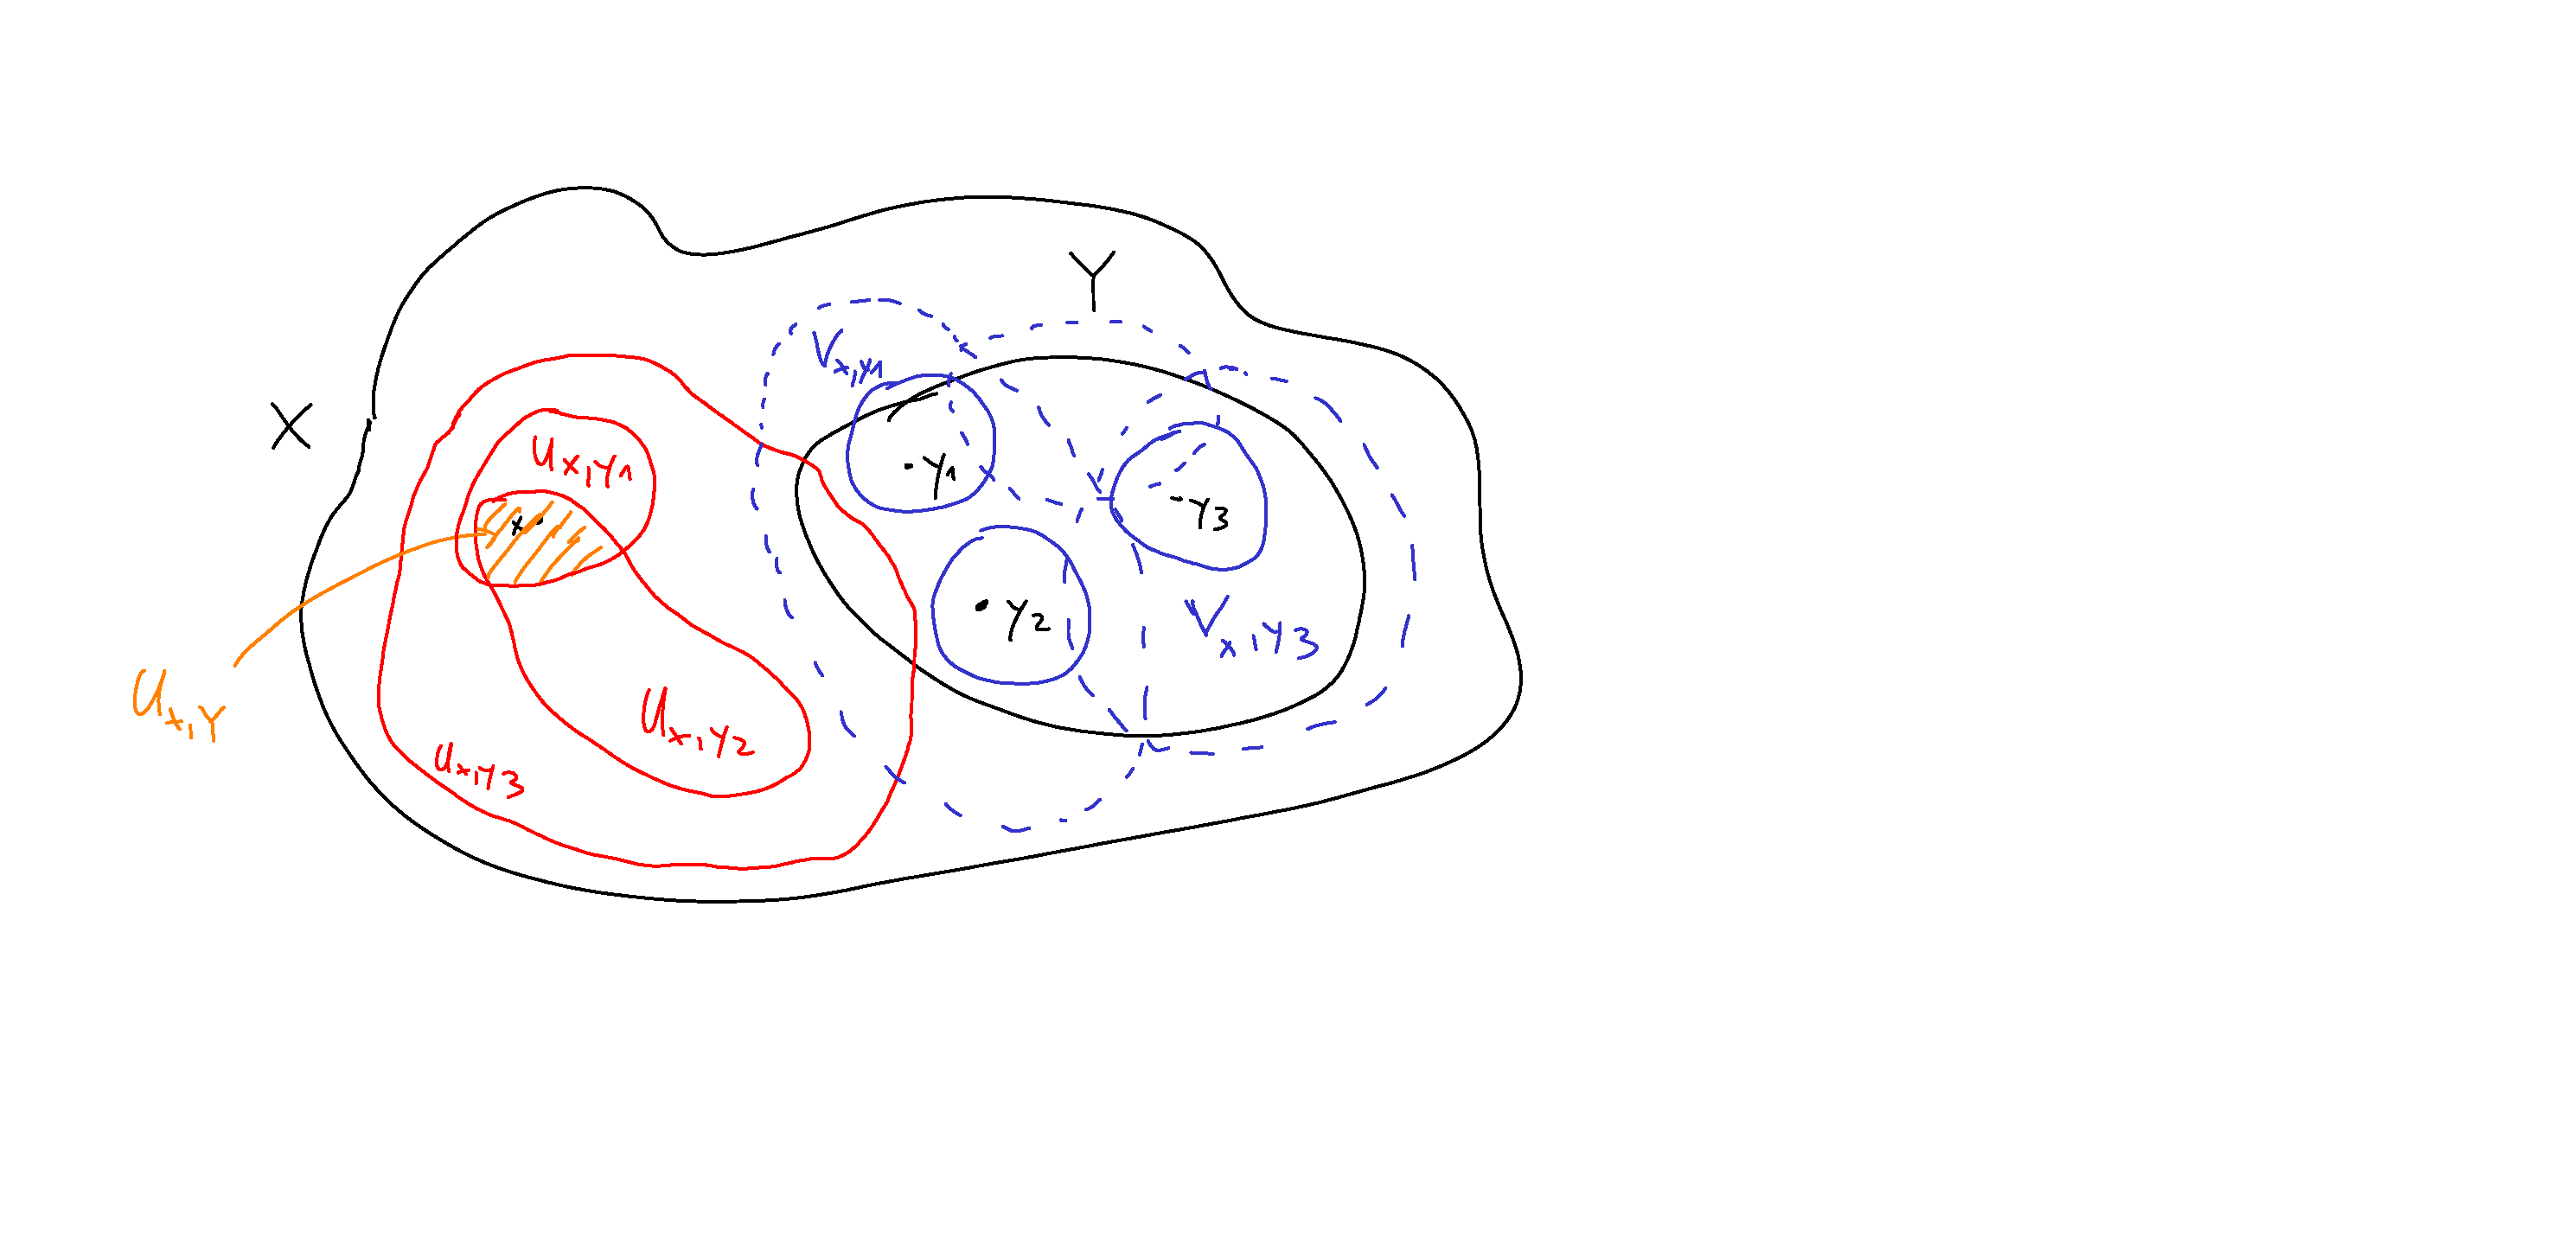
\includegraphics[scale=0.4]{figures/Lemma5.5.pdf}
    \caption{Skizze zum Beweis von Lemma \ref{lm:in-hausdorff-raum-sind-kompakte-mengen-t3}}
\end{figure}
\begin{proof}[Beweis von \autoref{thm:kompakte-menge-in-hausdorff-raum-ist-abgeschlossen}]
    Nach \autoref{lm:in-hausdorff-raum-sind-kompakte-mengen-t3} existieren $\forall x\in X \setminus Y$ ein $U_{x,Y}$ mit $x\in U_{x,Y}$ und $U_{x,Y} \cap Y = \emptyset$. Also ist
    \[
    X \setminus Y = \bigcup_{x\in X \setminus Y} U_{x,Y}
    .\] 
    offen und somit ist $Y$ abgeschlossen.
\end{proof}


\begin{example}['Gegenbeispiel' zu Satz \ref{thm:kompakte-menge-in-hausdorff-raum-ist-abgeschlossen}]
    Sei $G$ die Gerade mit zwei Urpsrüngen: \\
    Betrachte  $\R\cup \left \{0'\right\} $ mit $U$ Umgebung von  $a\in \R$ falls $\exists ε>0$ mit $(a-ε, a+ε)\subset U$ und $U$ Umgebung von  $0'$ und  $U$ Umgebung von  $0'$, falls  $\exists ε>0$ mit $(-ε,0 \cup (0,ε) \subset U$ und $0' \in U$. \\
    Wir können uns gewissermaßen  $0,0'$ gleichberechtigt vorstellen, nur dass die beiden Punkte verschieden sind. \\
    Dann ist  $[-1,1] \subset G$ kompakt (Übung!), aber nicht abegschlossen, da $0' \in G \setminus [-1,1]$ ist, dies aber keine Umgebung von $0'$ ist.
    \begin{figure}[H]
        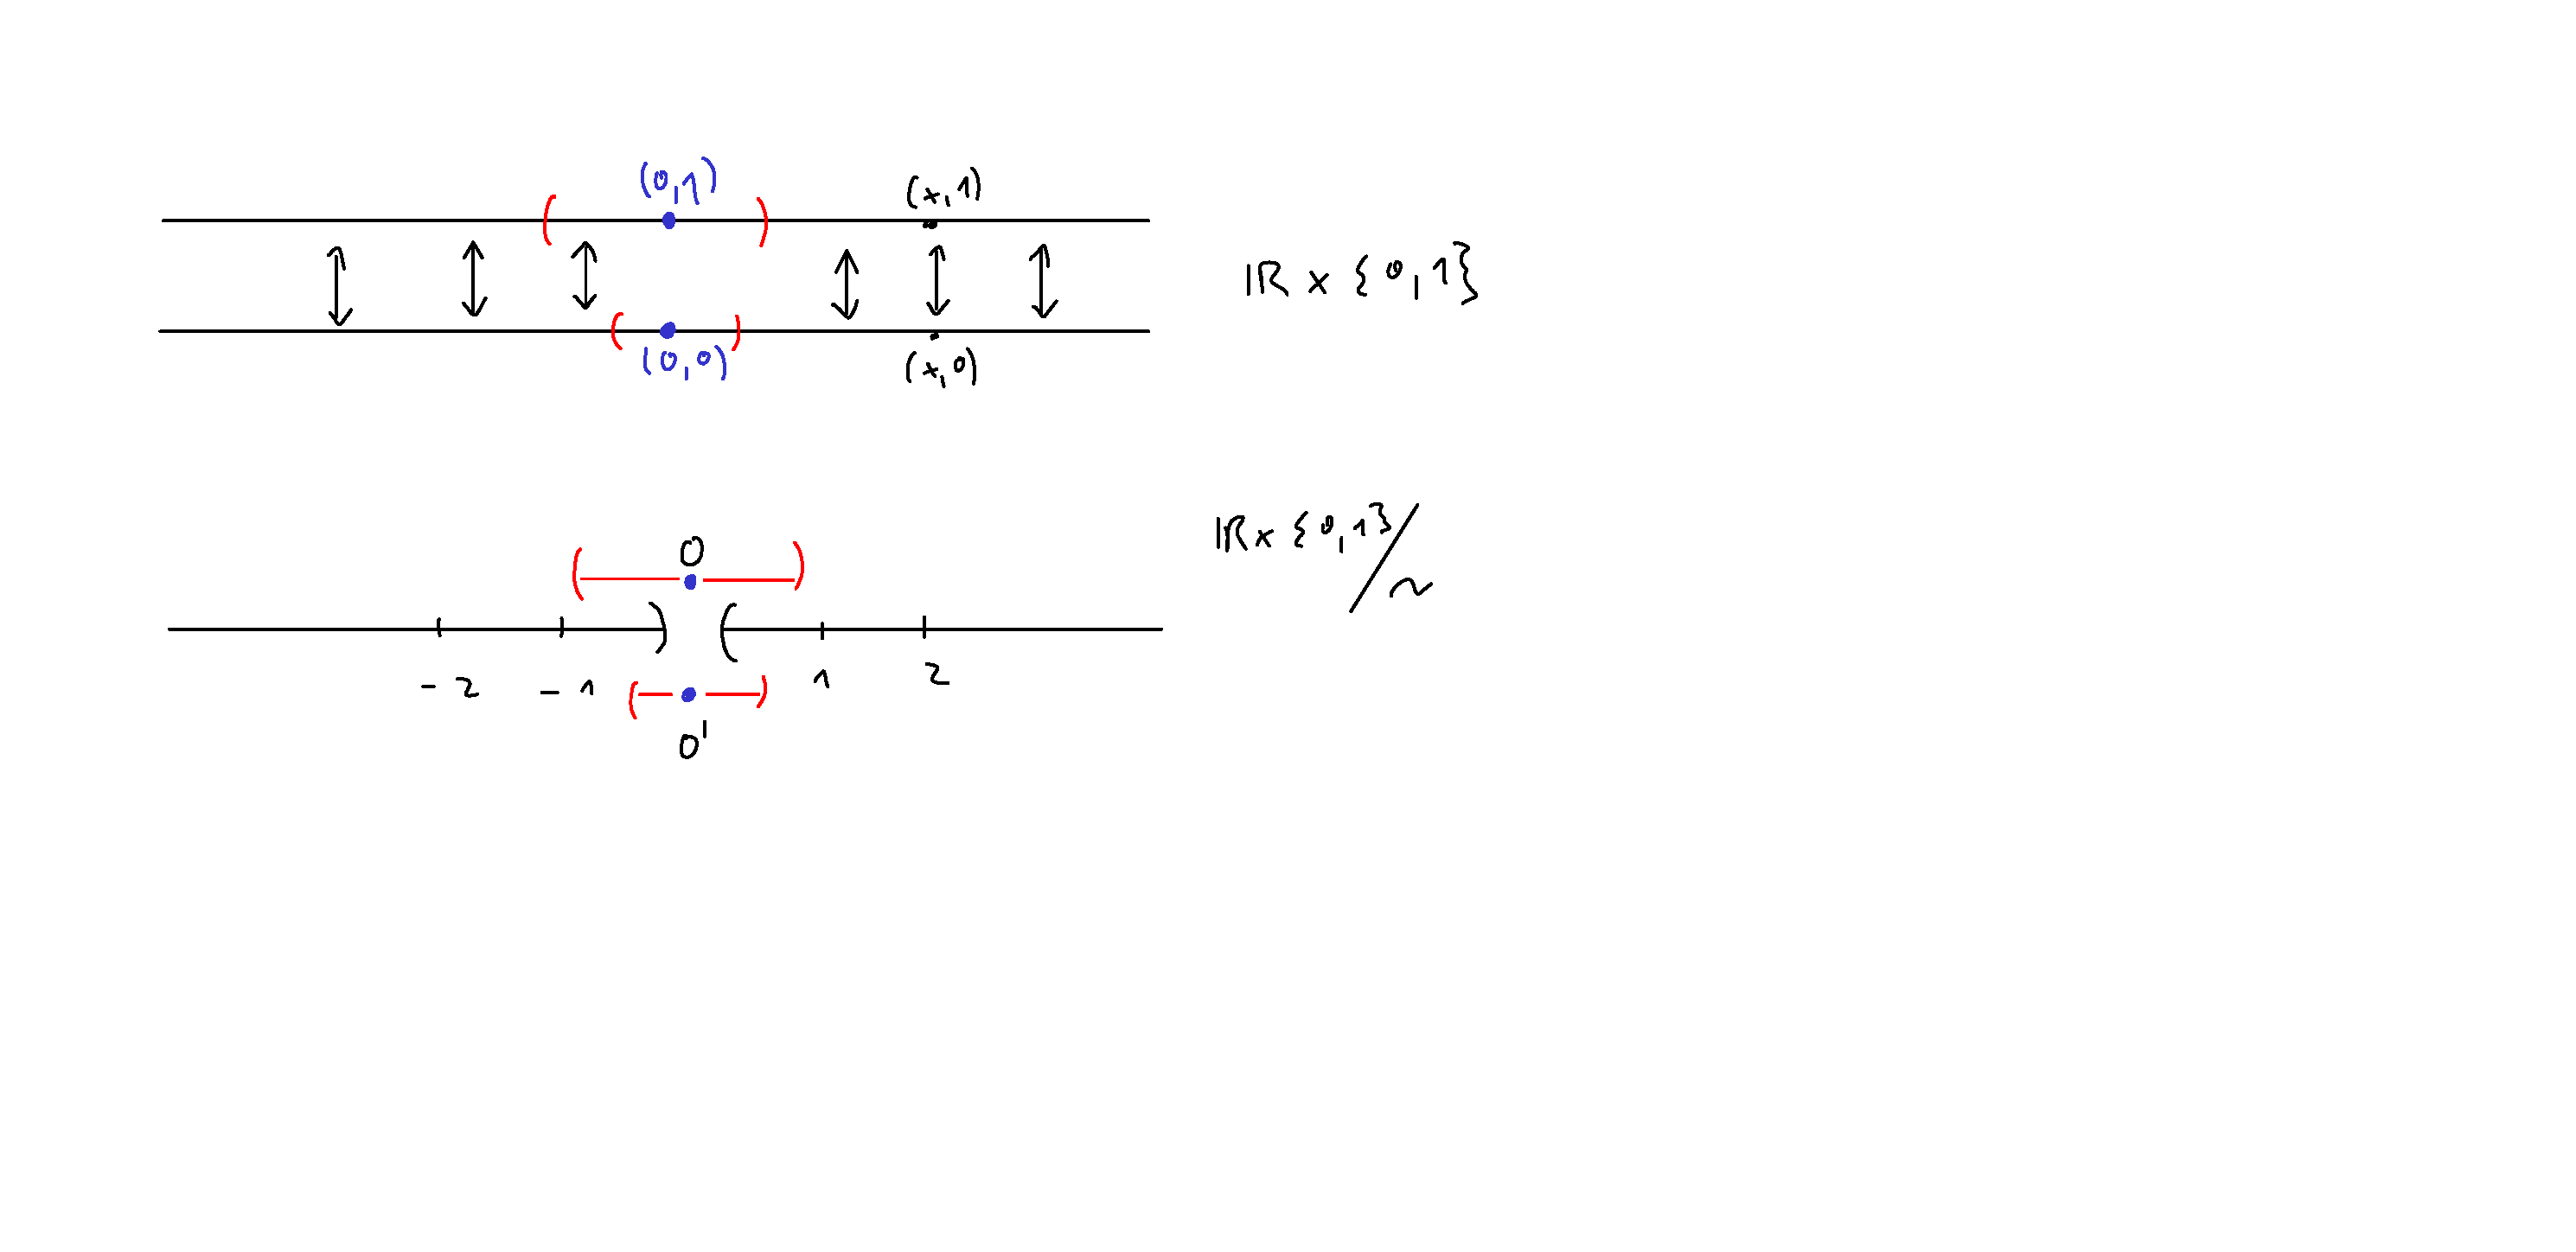
\includegraphics[scale=0.4]{figures/line-with-2-origins.pdf}
    \caption{Gerade mit 2 Ursprüngen}
    \end{figure}
\end{example}

Nun sind wir gewappnet für den
\begin{proof}[Beweis von \autoref{thm:heine-borel} (\nameref{thm:heine-borel})]
    '$2) \implies 1)$'. Sei $X\subset \R^n$ kompakt. Dann ist sie abgeschlossen nach \ref{thm:kompakte-menge-in-hausdorff-raum-ist-abgeschlossen}.
    Zudem ist $X\subset \bigcup_{x\in X} U(x,1)$ eine offene Überdeckung. Da $X$ kompakt finden wir endlich viele  $x_1,\ldots,x_n\in X$ mit
    \[
        X \subset \bigcup_{i=1}^n U(x_i,1)
    .\] 
    Also ist
    \[
        \diam(X) \leq  \max \left \{d(x_i,x_j)\right\} +2 < \infty
    .\] 
    und somit ist $X$ auch beschränkt. \\
    ' $1)\implies 2)$'. Da $X$ beschränkt ist,  $\exists m>0$ mit $X\subset [-m,m]^n\subset \R^n$. Da $X$ abgeschlossen ist, genügt es nach \autoref{thm:abgeschlossene-menge-in-kompaktem-raum-ist-kompakt} zu zeigen, dass  $[-m,m]^n$ kompakt ist. \\
    Wir führen einen Widerspruchsbeweis, nimm also an, dass  $[-m,m]^n$ nicht kompakt ist. Dann existiert eine offene Überdeckung  $\left \{U_i\right\} _{i \in I}$ ohne endliche Teilüberdeckung. \\
    \noindent\begin{minipage}{0.5\textwidth}
    Unterteile $[-m,m]^n$ in  $2^n$ gleich große Unterwürfel (halbiere jede Seite). Mindestens ein Unterwürfel hat keine endliche Teilüberdeckung. Unterteile diesen Würfel weiter und wähle wieder einen Unterwüfel, der keine endliche Teilüberdeckung hat. \\
    Wir erhalten eine Folge von Würfeln
     \[
         [-m,m]^n =     Q_0 \supset Q_1 \supset Q_2 \supset Q_3 \supset \ldots
    .\] 
    die jeweils keine endliche Teilüberdeckung durch $U_i's$ besitzen. \\
    \end{minipage}
    \begin{minipage}{0.5\textwidth}
\begin{tikzpicture}
    \draw (-2,-2) -- (-2,2) node[near end, anchor=east]{$Q_0$}-- (2,2) -- (2,-2) -- (-2,-2);
    \draw[blue] (-2,0) -- (2,0);
    \draw[blue] (0,-2) -- (0,2);
    \draw[blue,very thick] (0,0) -- (2,0) -- (2,2) node[anchor=west]{$Q_1$} -- (0,2) -- (0,0) ; 
    \draw[red] (1,0) -- (1,2);
    \draw[red] (0,1) -- (2,1);
    \draw[red, very thick] (1,0) -- (1,1) node[anchor=west, midway]{$Q_2$} -- (2,1) -- (2,0) -- (1,0);
\end{tikzpicture}
    \end{minipage}
    Sei  $x_i \in Q_i$ beliebig. Dann ist $x_i$ eine Cauchy-Folge, also existiert $x = \lim_{i\to \infty} x_i$, und $x\in Q_0$, da $Q_0$ abgeschlossen. \\
    Somit gibt es ein $U_j$ mit  $x\in U_j$, da die $\left \{U_i\right\} _{i \in I}$ eine Überedeckung von $Q_0$ waren. Damit ist auch $U(x,ε) \subset U_j$ für ein $ε>0$. Wähle einen Würfel $x\in Q_k$ mit Kantenlänge $< \frac{ε}{\sqrt{n} }$, dann ist auch $Q_k \subset U(x,ε) \subset U_j$. Das ist aber ein Widerspruch dazu, dass $Q_k$ keine endliche Teilüberdeckung hat, \contra. \\
    Also ist  $Q_0$ kompakt.
\end{proof}



\begin{theorem}[Bilder kompakter Räume]\label{thm:bild-von-kompaktem-raum-ist-kompakt}
    Sei $f: X \to  Y$ stetig und surjektiv und $X$ kompakt. Dann ist auch  $Y$ kompakt. 
\end{theorem}
\begin{proof}
    Sei $\left \{U_i\right\} _{i \in I}$ offene Überdeckung von $Y$. Dann ist
     \[
         \left \{f^{-1}(U_i)\right\} _{i \in I}
    .\] 
    offene Überdeckung von $X$. Da  $X$ kompakt ist, gibt es  $J\subset I$ endlich mit $X = \bigcup_{j\in J} f^{-1}(U_j)$. Dann ist 
    \[
        Y = f(X) = \bigcup_{j\in J} f(f^{-1}(U_j)) = \bigcup_{j\in J} U_j
    .\] 
    Also existiert eine endliche Teilüberdeckung von $Y$.
\end{proof}
\begin{corollary}\label{cor:stetige-abbildung-von-kompaktem-raum-in-hausdorff-raum-ist-abgeschlossen}
    Sei $f: X \to  Y$ stetig, $X$ kompakt und  $Y$ Hausdorff. Dann ist  $f$ abgeschlossen, d.h. $\forall A\subset X$ abgeschlossen ist $f(A) \subset Y$ abgeschlossen.
\end{corollary}
\begin{proof}
    Sei $A\subset X$ abgeschlossen. Dann ist $A$ kompakt nach \autoref{thm:kompakte-menge-in-hausdorff-raum-ist-abgeschlossen}, also ist  $f(A)$ kompakt nach \autoref{thm:bild-von-kompaktem-raum-ist-kompakt} (weil $f: X \to f(A)\subset Y$ surjektiv ist). Damit ist dann $f(A)$ abegschlossen nach \autoref{thm:kompakte-menge-in-hausdorff-raum-ist-abgeschlossen}. \\
    Also sind Bilder abgeschlossener Mengen abgeschlossen.
\end{proof}

\begin{corollary}[Homöomorphismen]\label{cor:stetige-bijektion-von-kompaktem-raum-in-hausdorff-raum-ist-homöomorphismus}
    Ist $f: X \to  Y$ stetig und bijektiv, $X$ kompakt und  $Y$ Hausdorff, dann ist  $f$ ein Homöomorphismus.
\end{corollary}

\begin{proof}
    Wir müssen zeigen, dass die Umkehrabbildung stetig ist. Dafür reicht es zu zeigen, dass $\forall A\subset X$ abgeschlossen auch $f(A) = (f^{-1})^{-1}(A)$ abgeschlossen ist. Das gilt aber genau nach vorherigem \autoref{cor:stetige-abbildung-von-kompaktem-raum-in-hausdorff-raum-ist-abgeschlossen}
\end{proof}
\begin{corollary}\label{cor:abbildung-von-kompaktem-raum-in-hausdorff-raum-ist-quotientenabbildung}
    Sei $f: X \to  Y$ stetig und surjektiv, $X$ kompakt und  $Y$ Hausdorffsch. Dann trägt  $Y$ die Quotiententopologie, d.h.  $U\subset Y$ offen genau dann, wenn $f^{-1}(U) \subset X$ offen.
\end{corollary}

\begin{proof}
    '$\implies$' folgt wegen Stetigkeit. \\
    '$\impliedby$' Ist $f^{-1}(U) \subset X$ offen, dann ist $f^{-1}(Y \setminus U ) = X \setminus f^{-1}(U)$ abgeschlossen in $X$, also folgt aus dem \autoref{cor:stetige-abbildung-von-kompaktem-raum-in-hausdorff-raum-ist-abgeschlossen}
     \[
         Y \setminus U \stackrel{\text{surj.}}{=}   f\left( \underbrace{f^{-1}\left( Y \setminus U \right)}_{\text{abgeschlossen}}  \right) 
    .\] 
    abgeschlossen ist, also ist $U\subset Y$ offen.
\end{proof}
Kommen wir nun zum
\begin{proof}[Beweis von \autoref{thm:kreis-ist-quotientenraum-von-einheitsintervall}]
    Schon gezeigt:
        \begin{equation*}
        \begin{array}{c c l} 
            [0,1] & \longrightarrow & S_1 \\
        t & \longmapsto &  2^{2\pi it}
        \end{array}
    \end{equation*}
    ist stetig und surjektiv und faktorisiert über
    \[
        [0,1] /\left \{0,1\right\}  \to  S^1
    .\] 
    mit $f$ stetig und bijektiv. Wir wissen nun:  $S^1$ ist Hausdorffsch und  $[0,1]$ ist kompakt. Nach \autoref{thm:bild-von-kompaktem-raum-ist-kompakt} ist auch  $[0,1] /\left \{0,1\right\} $ kompakt, also ist $f$ ein Homöomorphismus nach \autoref{cor:stetige-bijektion-von-kompaktem-raum-in-hausdorff-raum-ist-homöomorphismus}
\end{proof}


\begin{theorem}\label{thm:kompakter-hausdorff-raum-ist-normal}
    Jeder kompakte Hausdorff-Raum ist normal.
\end{theorem}
\begin{proof}
    Seien $A,B\subset X$ abgeschlossen und disjunkt. Da $X$ kompakt ist, sind  $A,B$ kompakt. Nach Lemma 5.5 existieren  $\forall a\in A$ offene Mengen $U_a, V_a$ mit $a\in U_a, B\subset V_a$ und $U_a \cap V_a = \emptyset$. Dann ist
    \[
    A \subset \bigcup_{a\in A} U_a
    .\] 
    Also existieren $a_1,\ldots,a_n\in A$ mit
    \[
    A\subset \bigcup_{i=1}^n U_{a_i}
    .\] 
    wegen $A$ kompakt. Setze nun
    \[
    U_A := \bigcup_{i=1}^n U_{a_i}\supset A \qquad U_B := \bigcap_{i=1}^n V_{a_i}\supset B
    .\] 
$\forall i$ ist 
\[
    U_{a_i} \cap U_B \subset U_{a_i} \cap V_{a_i} = \emptyset
.\] 
und daraus folgt, dass
\[
U_A \cap U_B = \emptyset
.\] 
\end{proof}

\begin{theorem}[Quotientenräume von Hausdorffräumen]\label{thm:quotientenraum-von-hausdorffraum-ist-hausdorff-gdw-projektion-abgeschlossen}
    Sei $X$ kompakt und Hausdorffsch, $q: X \to  Z$ surjektiv, wobei  $Z$ die Quotiententopologie trage. Dann sind äquivalent: 
    \begin{enumerate}[1)]
        \item $Z$ ist Hausdorffsch
        \item  $q$ ist abgeschlossen
    \end{enumerate}
\end{theorem}
\begin{proof}
    Die Richtung '$1) \implies 2)$' ist genau \autoref{cor:stetige-abbildung-von-kompaktem-raum-in-hausdorff-raum-ist-abgeschlossen} \\
    '$2)\implies_1)$': Jedes $z\in Z$ hat ein Urbild $x\in X$ unter $q$. Es ist  $\left \{x\right\} \subset X$ abgeschlossen, da $X$ hausdorffsch. Wegen  $q$ abgeschlossen folgt nun, dass auch
    \[
        \left \{z\right\}  = q(\left \{x\right\} )
    .\] 
    abgeschlossen ist. \\
    Wir nennen Teilmenge $W\subset X$ heißt \vocab[Menge!saturiert]{saturiert}, falls $W = q^{-1}(q(W))$ (insbesondere sind alle Urbilder saturiert, und $\iff  \forall x\in X \setminus W : g(x) \in Z \setminus g(W)$). \\
\begin{remark}
    Sei $U\subset X$ offen und saturiert, dann ist $q(U)$ offen. Hierzu schreibe
    \[
        U = q^{-1}(q(U)) \implies q(U) \text{ offen}
    .\] 
\end{remark}
Seien $y\neq z\in Z$. Dann sind $\left \{y\right\} ,\left \{z\right\} $ abgeschlossen und disjunkt. Dann sind auch
\[
    A = q^{-1}(y) \qquad B = q^{-1}(z)
.\] 
abgeschlossen und disjunkt (in  $X$). Nach Annahme ist  $X$ kompakt und Hausdorff, also normal nach Satz \ref{thm:kompakter-hausdorff-raum-ist-normal}. Also existieren  $U_1,U_2\subset X$ offen mit $A\subset U_1,B\subset U_2$ und $U_1 \cap U_2 = \emptyset$. Setze
\[
    V_1 := X \setminus q^{-1}(q(X\setminus U_1)) \qquad V_2 := X \setminus q^{-1}(q(X\setminus U_2))
.\] 
\begin{claim}
    Es sind $V_1,V_2$ offen, disjunkt und saturiert und $A\subset V_1$ sowie $B\subset V_2$.
\end{claim}
\begin{subproof}
    Nächstes Mal.
\end{subproof}
Es folgt, dass $q(V_1),q(V_2)$ offen in $Z$ sind. Weiter ist  $y\in q(A)\subset q(V_1)$ und $z\in q(B) \subset q(V_2)$. Da $V_1,V_2$ disjunkt und saturiert, sind auch $q(V_1),q(V_2)$ disjunkt und wir sind fertig.
\end{proof}

    \lecture{5}{Di 27 Apr 2021 12:16}{}
\begin{proof}[Beweis der Behauptung]
    Es ist klar, dass $V_1, V_2$ offen sind. Für Disjunktheit sehen wir mit
    \[
        X \setminus U_i \subset  q^{-1}(q(X\setminus U_i))
    .\] 
    dass $U_i \supset X \setminus q^{-1}(q(X\setminus U_i)) = V_i$ 
    Für Saturiertheit genügt es zu sehen, dass $g^{-1}(C)$ saturiert ist für alle $C\subset Z$, da
    \[
        q^{-1}(q(q^{-1}(C))) = q^{-1}(C)
    .\] 
    weil $q$ surjektiv ist. Wegen
     \[
         A\subset U_1 \implies X \setminus A \supset X \setminus U_1 \implies q(X\setminus A) \supset q(X\setminus U_1) \implies \underbrace{q^{-1}(q(X\setminus A))}_{=X\setminus A} = q^{-1}q(X\setminus U_1)
    .\]
    Komplementbildung liefert unser gewünschtes Eregbnis.
\end{proof}


\begin{example}
    $\R \mathbb{P}^n$ ist Hausdorffsch. 
    \begin{proof}
        Es ist $\R \mathbb{P}^n \cong S^n / x \sim  - x$. Sei
        \[
        q : S^n \to  S^n / x\sim -x
        .\] 
    \end{proof}
    die Projektion. Da $S^n$ kompakt und Hausdorffsch ist, ist  $\R \mathbb{P}^n$ Hausdorffsch genau dann, wenn $q$ abgeschlossen ist. Ist  $A\subset S^n$, so ist $q^{-1}(Q(A)) = A \cup -A$. \\
Da $-: S^n \to  S^n$ ein Homöomorphismus ist, ist $-A$ abgeschlossen, wenn  $A$ abgeschlossen ist. Dann ist auch  $A \cup -A$ abgeschlossen.
\end{example}
\begin{corollary}
    Sei $\sim $ auf $D^n = \left \{x \in \R^n \mid  \lVert x \rVert \leq 1\right\} $ erzeugt durch $x \sim -x$ für alle $x\in S^{n-1}\subset D^n$. Dann ist
    \[
    D^n / \sim  \cong \R \mathbb{P}^n
    .\] 
    Insbesondere ist 
    \[
        \R\mathbb{P}^1 \cong D^1 / \left \{-1,1\right\} \cong [0,1] / \left \{0,1\right\}  \cong S^1
    \]
    \label{cor:}
\end{corollary}
\begin{proof}
    Betrachte die stetige Abbildung
        \begin{equation*}
        f: \left| \begin{array}{c c l} 
        D^n & \longrightarrow & S^n \\
        x& \longmapsto &  (x,\sqrt{1-\lVert x \rVert ^2}) 
        \end{array} \right.
    \end{equation*}

    \todo{        Skizze einfügen für 'ausbeulen' der Abbildung.}
    Wir erhalten das Diagramm
    \begin{figure}[h]
        \centering
    \begin{tikzcd}
        D^n \ar{r} \ar{d} & S^n \ar{d} \\
    D^n / \sim \ar[dashed,swap]{r}{\overline{f}} & S^n / (x\sim -x) \cong \R\mathbb{P}^n
    \end{tikzcd}
    \end{figure}
    Wir sehen leicht, dass $\overline{f}$ bijektiv ist. Da $D^n$ kompakt, ist auch  $D^n / \sim $ kompakt, und $\R\mathbb{P}^n$ ist Hausdorffsch, also handelt es sich um einen Homöomorphismus (mit \ref{cor:compact-to-hausdorff-is-homeomorphism})
\end{proof}

\begin{corollary}
    Sei $X$ kompakt und Hausdorffsch und  $A\subset X$. Dann sind äquivalent
    \begin{enumerate}[1)]
        \item $X / A$ ist Hausdorffsch
        \item  $A$ ist abgeschlossen.
    \end{enumerate}
\end{corollary}
\begin{proof}
    '$1)\implies_2)$'. Ist $X // A$ Hausdorffsch, so ist die einpunktige Menge $\left \{A\right\} $ abgeschlossen (nach \ref{thm:point-in-hausdorff-space-is-closed}). Also ist $q^{-1}(A) = A$ abgeschlossen. \\
    '$2)\implies 1)$' Nach \ref{thm:quotient-space-of-compact-hausdorff-space} genügt es zu zeigen, dass $q: X \to  X / A$ abgeschlossen ist. Für $B\subset X$ abgeschlossen ist
    \[
        q^{-1}(q(B)) = \begin{cases}
            B & \text{falls } B\cap A = \emptyset \\
            B \cup A & \text{falls }B \cap  A \neq  \emptyset
        \end{cases}
    .\] 
    abgeschlossen, weil $A$ abgeschlossen ist. 
\end{proof}


\begin{example}
    \begin{enumerate}[a)]
        \item
Es ist $D^n / S^{n-1}$   Hausdorffsch. Alternativ können wir auch sehen, dass $D^n / S^{n-1} \cong S^n$ ist. Hierzu betrachte die Projektion:
    \begin{equation*}
    \begin{array}{c c l} 
    D^n & \longrightarrow & S^n \\
    x & \longmapsto &  \begin{cases}
        (2x, \sqrt{1-\lVert 2x \rVert ^2} & 0 \leq  \lVert x \rVert \leq \frac{1}{2}  \\
        \left( \frac{2-2\lVert x \rVert }{\lVert x \rVert }\cdot x, - \sqrt{1-(2-2\lVert x \rVert )^2}  \right) & \frac{1}{2} \leq  \lVert x \rVert  \leq 1
    \end{cases}
    \end{array}
\end{equation*}
Diese ist stetig, denn falls $\lVert x \rVert =\frac{1}{2}$ ist
\item Wir erhalten nun eine Abbildung 
\[
\frac{2-2\lVert x \rVert }{\lVert x \rVert } = \frac{2-1}{\frac{1}{2}} = 2
.\] 
und
\[
    \sqrt{1-\lVert 2x \rVert ^2} = \sqrt{1-1} =0 = - \sqrt{0} = -\sqrt{1-(2-2\lVert x \rVert )^2}  
.\] 
Ist $\lVert x \rVert =1$, so ist
 \[
\frac{2-2\lVert x \rVert }{\lVert x \rVert } = 0
.\] 
und somit ist $f(x) = (0,-1) \in \R^n \times \R$. Also faktorisiert $f$ über  $\overline{f} : D^n / S^{n-1} \to  S^n$. Wir sehen wieder leicht, dass $\overline{f}$ stetige Bijektion ist. Da $D^n / S^{n-1}$ kompakt und $S^n$ Hausdorffsch, folgt wieder, dass  $\overline{f}$ ein Homöomorphismus ist. \\
    \begin{tikzcd}
        S^n \ar{r}{q} & S^n / (x\sim -x) \cong \R\mathbb{P}^n \cong D^n / (x\sim -x) \ar{r} &  D^n / S^{n-1} \cong S^n
    \end{tikzcd}
    \end{enumerate}
\end{example}
\todo{Abbildung skizzieren}

\def\Base{\mathcal{S}} %temporary
\section{Basen und Subbasen}
\begin{definition}
    Sei $(X, \mathcal{O})$ ein topologischer Raum. Sei $\Base \subset \mathcal{O}$ eine Menge offener Mengen. Dann heißt $\Base$
    \begin{description}
        \item[\vocab{Basis}], falls $\forall U\subset \mathcal{O}$ existiert $S_i \in \Base$ mit $U = \bigcup_{i\in I} S_i$ 
        \item[\vocab{Subbasis}], falls $\forall U\in \mathcal{O}$ existieren $I, K_i$ endlich sowie  $S_k \in  \Base$ mit 
            \[
            U = \bigcup_{i\in I} \bigcap_{k\in K_i} S_k 
            .\] 
    \end{description}
\end{definition}
\begin{remark}
Ist     $\Base$ eine Basis, so ist $\Base$ eine Subbasis.
\end{remark}
\begin{example}
    Ist $(X,d)$ ein metrischer Raum, so ist
     \[
         \Base = \left \{U(x,ε) \mid  x\in X, ε>0\right\} 
    .\] 
    eine Basis der Topologie.
\end{example}
\begin{theorem}
    Sei $X$ eine Menge,  $\Base \subset \mathcal{P}(X)$ eine Menge von Teilmengen. Dann existiert genau eine Topologie auf  $X$, für die  $\Base$ eine Subbasis ist, nämlich:
     \[
    \mathcal{O} = \left \{U\subset X \mid  U = \bigcup_{i \in  I} \bigcap_{k\in K_i} S_k \text{ mit } \abs{K_i}<\infty, S_k \in  \Base  \right\} 
    .\] 
\end{theorem}
\begin{proof}
    Übung.
\end{proof}
\begin{notation}
    Wir nennen $\mathcal{O}$ die \vocab{von $\Base$ erzeugte Topologie}.
\end{notation}
\begin{lemma}
    Sei $f: X \to  Y$ eine Abbildung zwischen topologischen Räumen, $\Base$ eine Subbasis von $Y$. Dann sind äquivalent:
    \begin{enumerate}[1)]
        \item $f$ ist stetig
        \item  $f^{-1}(S)$ ist offen für alle $S\in \Base$
    \end{enumerate}
\end{lemma}
\begin{proof}
    '$1) \implies 2)$' ist klar, da Subbasiselemente offen sind. \\
    '$2) \implies 1)$'. Sei $U \subset Y$ offen, dann $\exists K_i$ endlich und $S_k \in \Base$ mit
    \[
    U = \bigcup_{i \in  I} \bigcap_{k\in K_i} S_k
    .\] 
    Dann ist aber genau
    \[
        f^{-1}(U) = \bigcup_{i \in  I} \bigcap_{k\in K_i} \underbrace{f^{-1}(S_k)}_{\text{offen}} 
    .\] 
    offen, weil endliche Schnitte und beliebige Vereinigung offener Mengen offen sind. Also ist $f$ stetig.
\end{proof}

\begin{theorem}
    Eine Subbasis $\Base$ von  $(X, \mathcal{O})$ ist eine Basis genau dann, wenn
    \[
    \forall S_1, S_2 \in \Base \;\exists S_i \in \Base \colon S_1 \cap S_2 = \bigcup_{i \in I} S_i
    .\] 
\end{theorem}
\begin{proof}
'$\implies$'    Da $S_1,S_2 \in \Base$ sind diese offen. Dann ist auch $S_1\cap S_2$ offen. Ist $\Base$ Basis, dann gibt es also  $S_i \in  \Base$ mit 
\[
S_1 \cap  S_2 = \bigcup_{i \in  I} S_i
.\] 
'$\impliedby$' Angenommen, $U\subset X$ ist offen und von der Form
\[
    U = \bigcup_{i \in  I} \left( \bigcap_{k\in K_i} S_k \right) 
.\] 
mit $K_i$ endlich und  $S_k \in  \Base$. Nach Annahme ist
\[
\bigcap_{k\in K_i} = \bigcup_{j\in J_i} S_j  
.\] 
und damit ist
\[
U = \bigcup_{i\in I} \bigcup_{j\in J_i} S_j  
.\] 
\end{proof}
\begin{remark}
    Nach Annahme ist eigentlich erstmal der Schnitt von 2 Mengen die Vereinigung von $S_i$. Allerdings kann man dies per Induktion leicht auf  $n$ Teilmengen verallgemeinern, wenn wir
     \[
         \bigcap_{k=1}^n S_k = S_1 \cap  \bigcap_{k=2}^{n} S_k = S_1 \cap \bigcup_{i\in I} S_i = \bigcap_{i\in I} (S_i \cap S_k) = \bigcup_{i\in I} \bigcup_{j\in J_i} S_j  
    .\]
    für geeignete $S_i, S_j\in \Base$ schreiben.
\end{remark}
\begin{theorem}
    \label{thm:alexander}
    Sei $X$ ein topologischer Raum und  $\Base$ eine Subbasis. Dann ist  $X$ kompakt genau dann, wenn jede Überdeckung durch Elemente aus  $\Base$ eine endliche Teilüberdeckung besitzt.
\end{theorem}
\begin{proof}
    '$\implies$' ist klar. \\
    '$\impliedby$' Angenommen, $X$ ist nicht kompakt, dann betrachte die Menge
     \[
    \mathcal{C} := \left \{U \mid  U \text{ offene Überdeckung \underline{ohne} endliche Teilüberdeckung}\right\} \neq \emptyset
    .\] 
    Es ist $\mathcal{C}$ partiell geordnet, indem wir $U\leq U'$ für $U\subset U'$ setzen. \\
    Ist $U_1\subset U_2\subset \ldots$ eine Kette, so ist $\bigcup_{U_i}\in \mathcal{C}$, denn
    \begin{itemize}
        \item Offenbar ist $\bigcup_{i \in  I} U_i$ eine offene Überdeckung.
        \item Hat $\bigcup_{i \in  I} U_i$ eine endliche Teilüberdeckung, so ist diese schon in einem $U_i$ enthalten, und damit enthielte auch dieses  $U_i$ bereits eine endliche Teilüberedckung \contra
    \end{itemize}
Wir können also das Lemma von Zorn anwenden, und somit existiert ein maximales Elment $U\in \mathcal{C}$.
\begin{claim}
    Ist $V\subset X$ offen und  $V\not\in U$, so hat $U\cup \left \{V\right\} $ eine endliche Teilüberdeckung
\end{claim}
\begin{subproof}
    Sonst wäre $U \cup \left \{V\right\} \in \mathcal{C}$ und somit wäre $U$ nicht maximal
\end{subproof}
\begin{claim}
    $U \cap \Base$ ist keine Überdeckung
\end{claim}
\begin{subproof}
    Sonst hätte $U$ eine endliche Teilüberedckung nach Annahme.
\end{subproof}
Wegen Behauptung 2 existiert $x\in X$, der nicht von $U \cap \Base$ überdeckt wird. Sei $W\in U$ mit $x\in W$. Da $W$ offen ist, folgt
 \[
W = \bigcup_{i \in  I} \bigcap_{k\in K_i} S_k
.\] 
mit $K_i$ endlich und  $S_k \in \Base$. Dann existieren also $S_1,\ldots,S_n$ mit 
\[
x \in  \bigcap_{i=1}^n S_i \subset W 
.\] 
Da $x$ nicht von  $U \cap \Base$ überdeckt wird, ist $S_i \not\in U$. Aus der ersten Behauptung wissen wir nun aber, dass es $U_1^i, \ldots, u_{n_i}^i \in U$ mit
\[
\left \{U_j ^i\right\} _{j=1}^n \cup \left \{S_i\right\}  \quad \text{ ist Überdeckung von } X
.\] 
Sei nun 
\[
\hat{U} := \left \{U_j ^i \mid  1\leq i\leq n, 1\leq j\leq n_i\right\} \subset U
.\] 
Für alle $i$ gilt also
 \[
X \subset \bigcup_{V\in \hat{U}} V \cup S_i 
.\] 
Also folgt
\[
X \setminus \bigcup_{V\in \hat{U}} V \subset S_i 
.\] 
und damit ist auch
\[
X\setminus \bigcup_{V\in \hat{U}} V \subset S_1 \cap \ldots \cap S_n \subset W \in U 
.\] 
Also ist $\hat{U}\cup \left \{W\right\} $ eine endliche Teilüberdeckung von $U$, \contra.
\end{proof}

    \lecture{6}{Do 29 Apr 2021 10:01}{}
\section{Produkte}
\begin{definition}
    Seien $X_1,X_2$ topologische Räume. Die \vocab{Produkttopologie} auf $X_1\times X_2$ ist die Topologie erzeugt von
    \[
    \mathcal{B} = \left \{U_1\times U_2 \mid  U_1\subset X_1 \text{ offen }, U_2\subset X_2\text{ offen}\right\} 
    .\] 
\end{definition}
\begin{example}
    Seien $(X_1,d_1)$ und $(X_2,d_2)$ metrische Räume. Auf $X_1\times X_2$ haben wir die Metriken definiert durch
    \[
        \begin{split}
            d_{\max} ((x_1,x_2),(y_1,y_2) &:= \max \left \{d_1(x_1,y_1), d_2(x_2,y_2)\right\}  \\
            \tilde{d}_1((x_1,x_2),(y_2,y_2)) &:= d_1(x_1,y_1) + d_2(x_2,y_2) \\
            \tilde{d}_2((x_1,x_2),(y_1,y_2)) &:= \sqrt{d_1(x_1,y_1)^2 + d_2(x_2,y_2)^2} 
        \end{split}
    .\] 
    Dies Metriken sind paarweise äquivalent (leicht zu prüfen). Zudem sind $ε$-Bälle in  $d_{\max}$ gegeben durch
    \[
        U_{d_{\max}}((x_1,x_2),ε)) = U_{d_1}(x_1,ε) \times U_{d_2}(x_2,ε)
    .\] 
    D.h. die von $d_{\max}$ induzierte Topologie ist die Produkttopologie.
\end{example}
\begin{example}
    Es ist $\R^2 \cong \R \times \R$, wobei wir auf der linken Seite die Standardtopologie und auf der rechten Seite die Proudkttopologie meinen.
\end{example}
\begin{remark}
    $\mathcal{B}$ ist per Definition eine Subbasis der Produkttopologie, in der Tat handelt es sich jedoch sogar um eine Basis:
    \begin{proof}
        Seien $U_1\times U_2$ sowie $V_1\times V_2\in \mathcal{B}$ Basiselemente. Wir stellen fest, dass
        \[
            (U_1\times U_2)\cap (V_1\times V_2) = (U_1\cap U_2) \times (V_1\cap V_2)
        .\] 
        das Produkt zweier Basiselemente ist, und somit sind wir fertig.
    \end{proof}
\end{remark}
\begin{theorem}
    Die Projektionen
        \begin{equation*}
        p_x: \left| \begin{array}{c c l} 
        X\times Y & \longrightarrow & X \\
        (x,y) & \longmapsto &  x
        \end{array} \right.
        \qquad
        p_Y: \left| \begin{array}{c c l} 
            X\times Y & \longrightarrow & Y \\
            (x,y) & \longmapsto	 &  y
        \end{array} \right.
    \end{equation*}
    sind stetig und offen
\end{theorem}
\begin{proof}
    Sei $U\subset X$ offen. Dann ist $p_X^{-1}(U) = U\times Y\in \mathcal{B}$, also offen. Analoges gilt für $p_Y$. \\
    Sei $U\subset X\times Y$ offen. Dann können wir $U$ schreiben als
     \[
    U = \bigcup_{i \in  I} U_i \times V_i
    .\] 
    OBdA können wir $V_i \neq  \emptyset$ annehmen. Dann ist aber
    \[
        P_X(U) = \bigcup_{i \in  I} p_X(U_i \times V_i) = \bigcup_{i \in  I} U_i \subset X
    .\] 
    offen, also ist $p_X$ offen.
\end{proof}
\begin{remark}
    Die Projektion $p_X$ ist i.A. nicht abgeschlossen.
     \begin{proof}
         Betrachte $A = \left \{\left( \frac{1}{n},n \right) \in \R^2 \mid  n \in \N_{>0}\right\} \subset \R^2$  abgeschlossen. Dann ist aber $p_1(A) = \left \{\frac{1}{n}\mid n \in \N_{>0}\right\} \subset \R$ \underline{nicht} abgeschlossen.
    \end{proof}
\end{remark}
\begin{theorem}
    Ist $Y$ kompakt, so ist  $p_X$ abgeschlossen. 
\end{theorem}
\begin{proof}
    Sei $A\subset X\times Y$ abgeschlossen. Wir müssen zeigen, dass $X \setminus p_X(A)$ offen ist, also wähle $x\in X \setminus p_X(A)$. Für alle $y\in Y$ ist $(x,y) \not\in A$ (sonst wäre $x\in p_X(A)$, also gibt es 
    \[
        x\in U_y \subset X \quad y\in V_y \subset Y \text{ offen} \colon (U_y \times V_y) \cap A = \emptyset
    .\] 
    Damit sind die $\left \{V_y\right\} _{y\in Y}$ eine offene Überdeckung von $Y$ und  wir finden mit  $Y$ kompakt eine endliche Teilüberdeckung  $V_{y_1},\ldots,V_{y_n}$ von $Y$. Setzen wir nun
     \[
    U := \bigcap_{i =1}^n U_{y_i} 
    .\] 
    so ist $U\subset X$ offen als endlicher Schnitt und wir stellen mit
    \[
        U\times V_{y_i} \subset U_{y_i}\times V_{y_i}\subset (X\times Y) \setminus A
    .\] 
    fest, dass bereits $U\times Y\subset (X\times Y)\setminus A$ (weil die $V_{y_i}$ bereits $Y$ überdecken). Nun muss aber bereits
     \[
         U\subset X \setminus p_X(A)
    .\] 
    gelten, und damit ist dieses $U$ eine offene Umgebung von  $x\in X \setminus p_X(A)$.
\end{proof}
\begin{lemma}
    Seien $X,Y$ topologische Räume. Die Menge
     \[
    \mathcal{S} = \left \{U\times Y, X\times V \mid  U\subset X \text{ offen}, V\subset Y \text{ offen}\right\} 
    .\] 
    ist eine Subbasis der Produkttopologie.
\end{lemma}
\begin{proof}
    Sei $W\subset X\times Y$ offen. Dann gibt es nach der Definition der Produkttopologie $U_i\subset X, V_i\subset Y$ offen mit
    \[
        W = \bigcup_{i \in  I} (U_i \times V_i)
    .\] 
    Also ist bereits
    \[
        W = \bigcup_{i \in  I} ((U_i\times Y) \cap (X\times V_i))
    .\] 
    eine Vereinigung endlicher Schnitt von unseren Subbasiselementen. \\
    Umgekehrt ist klar, dass alle Elemente aus $\mathcal{S}$ auch offene Mengen in der Produkttopologie sind, da $\mathcal{S} \subset \mathcal{B}$.
\end{proof}
\begin{theorem}[Universelle Eigenschaft des Produkts]
    Seien $A,X_1,X_2$ topologische Räume sowie $f_i: A \to  X_i$. Dann ist die Abbildung
        \begin{equation*}
            (f_1\times f_2) =: f: \left| \begin{array}{c c l} 
        A & \longrightarrow & X_1\times X_2 \\
        a & \longmapsto &  (f_1(a),f_2(a))
        \end{array} \right.
    \end{equation*}
    stetig genau dann, wenn $f_1,f_2$ stetig sind. \\
    \begin{tikzcd}
        & & X_1 \\
        A \ar[dashed]{r}{f} \ar[bend left = 30]{rru}{f_1} \ar[swap, bend right = 30]{rrd}{f_2} & X_1\times X_2 \ar{ur}{p_1} \ar{dr}{p_2} \\
                                                                              & & X_2
    \end{tikzcd}
\end{theorem}
\begin{proof}
    Es ist $f_i = p_i \circ  f$. Ist $f$ stetig, so ist  $f_i$ stetig als Verknüpfung stetiger Funktionen. \\
    Angenommen, es sind $f_1,f_2$ stetig. Wir müssen zeigen, dass für alle $U_1\times U_2\subset X_1\times X_2$ mit $U_i\subset X_i$ offen auch $f^{-1}(U_1\times U_2)$ offen ist. Hierzu stellen wir aber fest, dass
    \[
        f^{-1}(U_1\times U_2) = f_1^{-1}(U_1) \cap  f_2^{-1}(U_2)
    .\] 
    offen ist.
\end{proof}
\begin{example}
    \begin{enumerate}[a)]
        \item Wir behaupten, dass
            \[
                \R^{n+1} \setminus \left \{0\right\} \cong S^n \times (0,\infty) \cong S^n \times \R
            .\] 
            ist. Betrachte hierzu
                \begin{equation*}
                \varphi : \left| \begin{array}{c c l} 
                    \R^{n+1}\setminus \left \{0\right\}  & \longrightarrow & S^n\times (0,\infty) \\
                    x & \longmapsto &  \left( \frac{x}{\lVert x \rVert _2}, \lVert x \rVert _2 \right) 
                \end{array} \right.
            \end{equation*}
            Wir sehen nun mit der universellen Eigenschaft sofort, dass es sich um eine stetige Abbildung handelt. Zudem haben wir die Umkehrfunktion
                \begin{equation*}
                \begin{array}{c c l} 
                    S^n \times (0,\infty) & \longrightarrow & \R^{n+1}\setminus \left \{0\right\}  \\
                    (y,t) & \longmapsto &  t\cdot y
                \end{array}
            \end{equation*}
            Wir müssen noch prüfen, dass diese stetig ist (Übung), dann haben wir einen Homöomorphismus.
        \item $S^1\times S^1$ ist ein Torus. Betrachte hierzu
               \begin{equation*}
               \varphi : \left| \begin{array}{c c l} 
                   [0,1]^2 & \longrightarrow & S^1 \times S^1 \\
                   (s,t) & \longmapsto &  (e^{2\pi is}, e^{2\pi it})
               \end{array} \right.
           \end{equation*}
           $\varphi $ ist stetig und erfüllt $\varphi (s,0) = \varphi (s,1)$ sowie $\varphi (0,t) = \varphi (1,t)$. Also faktorisiert $\varphi $ wie gewünscht als
           \begin{tikzcd}
               \left[0,1\right]^2 \ar{r}{\varphi } \ar{d} & S^1 \times S^1  \\
               \left[0,1\right]^2 / \sim \ar[swap]{ur}{\varphi '}
           \end{tikzcd}
           wobei $\sim $ die Relation ist, die wir für die Konstruktion des Torus verwendet hatten. $\varphi '$ ist stetig und surjektiv nach der Universellen Eigenschaft, und wir sehen leicht, dass $\varphi '$ injektiv ist. Also ist $\varphi '$ stetig und bijektiv. Nun ist aber $[0,1]^2$ kompakt und $S^1 \times S^1$ Hausdorff (z.B. als metrisierbare Teilmenge von $\R^2 \times \R^2$), und somit ist $\varphi '$ ein Homöomorphismus nach \autoref{cor:compact-to-hausdorff-is-homeomorphism}
    \end{enumerate}
\end{example}
\begin{corollary}
    Seien $X,Y$ topologische Räume sowie  $y\in Y$. Dann ist $X\cong X\times \left \{y\right\} \subset X\times Y$ mittels $x \mapsto (x,y)$.
\end{corollary}
\begin{proof}
    Nenne diese Abbildung $f$, also
        \begin{equation*}
        f: \left| \begin{array}{c c l} 
        X & \longrightarrow & X\times Y \\
        x & \longmapsto &  (x,y)
        \end{array} \right.
    \end{equation*}
$f$ ist stetig, da sowohl  $\id_X$ als auc h
    \begin{equation*}
    c_Y: \left| \begin{array}{c c l} 
    X & \longrightarrow & Y \\
    x & \longmapsto &  y
    \end{array} \right.
\end{equation*}
stetig sind (mit universeller Eigenschaft). $f$ faktorisiert nun über  $X\times \left \{y\right\} \subset X\times Y$ und $f: X \to  X\times \left \{y\right\} $ ist offensichtlich bijektiv. Wir müssen also noch zeigen, dass $f$offen ist. \\
Sei  $U\subset X$ offen, dann ist $U\times Y \subset X\times Y$ offen. Es ist zudem
\[
    f(U) = U\times \left \{y\right\}  = U\times Y \cap  X \times \left \{y\right\}  \subset X\times \left \{y\right\} 
.\] 
in $X\times \left \{y\right\} $ offen.
\end{proof}
\begin{theorem}
    Seien $X,Y$ topologische Räume.
\begin{enumerate}[1)]
        \item Sind $X$ und  $Y$ Hausdorffsch, so auch  $X\times Y$
        \item Sind $X$ und $Y$ kompakt, so auch  $X\times Y$.
    \end{enumerate}
\end{theorem}
\begin{proof}
    \begin{enumerate}[1)]
        \item Seien $(x,y) \neq  (x',y' \in X\times Y$. Dann ist $x\neq x'$ oder $y\neq y'$. OBdA sei $x\neq x'$. Dann existieren $U,U'\subset X$ offen mit $x\in U, x'\in U'$ und $U\cap U' = \emptyset$, weil $X$ Hausdorffsch. Dann sind
            \[
                (x,y)           \in  U\times Y \qquad (x',y') \in U' \times Y
            .\] 
    jeweils offen, und ihr Schnitt ist
    \[
        (        U\times Y) \times (U'\times Y) = (U\cap U') \times Y = \emptyset
    .\] 
    Also ist $X\times Y$ Hausdorffsch.
\item Wir wollen den \nameref{thm:alexander} (\ref{thm:alexander}) verwenden. Sei $\mathcal{U}$ eine offene Überdeckung von  $X\times Y$ mit Elementen der Form $U\times Y$ oder $X\times V$. Sei
    \[
    W = \bigcup_{U\times Y \in \mathcal{U}} U \subset X \qquad W' = \bigcup_{X\times V \in \mathcal{U}} V \subset Y  
    .\] 
    Ist $W = X$, so existiert eine endliche Teilüberdeckung von  $\left \{U \mid  U\times Y \in \mathcal{U}\right\} $ durch $U_1,\ldots,U_n$. Dann ist bereits
    \[
    \left \{U_i \times Y \mid  i=1,\ldots,n\right\} 
    .\] 
    eine endliche Teilüberdeckung von $X\times Y$. Für $W' = Y$ verfahren wir genauso. Ist  $W \neq  X$ und $W'\neq Y$, so existiert $x\in X \setminus W, y\in Y \setminus W'$. Dann ist $(x,y)$ aber nicht von  $\mathcal{U}$ überdeckt, weil er von keinem $U\times Y$ und von keinem $X\times V$ überdeckt wird, \contra. \\
    Also finden wir in beiden Fällen eine endliche Teilüberdeckung.
    \end{enumerate}
\end{proof}
\begin{remark}
    Der Beweis geht auch ohne \autoref{thm:alexander}. Viel leichter: Es genügt, offene Überdeckungen bezüglich einer Basis zu betrachten (Spezialfall von Alexander, leicht zu zeigen), dann verfahren wir wie folgt: \\
    Sei $\mathcal{U}$ eine Überdeckung von $X\times Y$ mit Elementen aus $\mathcal{B}$. Dann gibt es eine endliche Teilüebredckung von $X\times \left \{y\right\} $. Sei diese $\left \{U_i^y \times V_i^y\right\} i=1^{n_y}$. Setze
    \[
        V_y := \bigcap_{i=1} ^{n_Y} V_i^{y}
    .\] 
    Dann ist dies eine Überdeckung von $X\times V_y$. Die $V_y$ bilden nun eine offene Überdeckung von  $Y$, also finden wir wieder eine endliche Teilüberdeckung durch  $V_{y_1}, \ldots, V_{y_n}$. Da wir aber die $X\times V_{y_i}$ jeweils endlich überdeckt haben, können wir nun auch $X\times Y$ endlich überdecken.
\end{remark}
\begin{definition}
Seien $X_1,\ldots,X_n$ topologische Räume. Dann definieren wir ihr Produkt rekursiv durch
\[
    X_1\times \ldots\times X_n := (X_1\times \ldots\times X_{n-1})\times X_n
.\] 
\end{definition}

\begin{lemma}
    Seien $X,Y$ topologische Räume mit Basen  $\mathcal{B}_X, \mathcal{B}_Y$. Dann ist
    \[
    \mathcal{B}_{X\times Y} := \left \{U\times V \mid  U\in \mathcal{B}_X, V\in \mathcal{B}_Y\right\} 
    .\] 
    eine Basis der Topologie auf $X\times Y$.
\end{lemma}
\begin{corollary}
    Die Mengen $U_1\times U_2\times \ldots.\times U_n$ mit $U_i\subset X_i$ offen sind eine Basis der Topologie auf $X_1\times \ldots\times X_n$. \\
    Insbesondere ist die Topologie unabhängig von der Klammerung.
\end{corollary}
\begin{proof}
    Setze $\mathcal{B}_{X_i} = \mathcal{O}_{X_i}$.
\end{proof}
\begin{proof}
    Seien $W\in X, W'\subset Y$ offen. Dann existieren $U_i \in \mathcal{B}_X$ sowie $V_j \in \mathcal{B}_Y$ mit
    \[
    W = \bigcup_{i \in  I} U_i \qquad W' = \bigcup_{j\in J} V_j 
    .\] 
    Dann ist bereits:
    \[
    W \times W' = \bigcup_{\substack{i\in I \\j\in J} } U_i \times V_j
    .\] 
    Ist nun $A\subset X\times Y$ beliebig offen, so gilt
    \[
    A = \bigcup W_i \times W_i' = \bigcup  \bigcup_{\substack{i\in I\\j\in J}  } U_i \times V_j
    .\] 
    Umgekehrt ist klar, dass die $U_i\times V_j$ offen in der Produkttopologie sind.
\end{proof}
\begin{theorem}
    Sei $X$ ein topologischer Raum. Dann ist  $X$ Hausdorffsch, genau dann, wenn
     \[
         \Delta_X := \left \{(x,x) \mid  x\in X\right\}  \subset X\times X
    .\] 
    abgeschlossen ist.
\end{theorem}
\begin{notation}
    Wir nennen $\Delta_X\subset X^2$  die \vocab{Diagonale von $X$}.
\end{notation}
\begin{proof}
'$\implies$' Nimm an, dass $X$ Hausdroffsch ist und sei  $(x,y) \in X \times X \setminus \Delta_X$, d.h. $x\neq y$. Dann existieren $x\in U_x,y\in U_y$ offen (in $X$), sodass  $U_x \cap  U_y = \emptyset$. Also ist
    \[
        (x,y)\in     U_x\times U_y \subset X\times X \setminus \Delta_X
    .\] 
    , denn wenn $(a,b) \in U_x \times U_y$, dann ist $a\neq b$. Also ist  $X\times X \setminus \Delta_X$ offen nach Definition. \\
    '$\impliedby$'    Nimm nun an, dass die Diagonale abgeschlosen ist. Seien $x,y\in X$ mit $x\neq y$ beliebig. Dann ist
    \[
        (x,y) \in X\times X \setminus \Delta_X = \bigcup_{i\in I} U_i \times V_i 
    .\] 
    Also ist $(x,y) \in U\times V \subset X\times X\setminus \Delta_X$ für eine Wahl von $U,V$. Dann ist aber  $x\in U, y\in V$ sowie $U\cap V = \emptyset$, denn wenn $a\in U\times V$, so $(a,a) \in U\times V \cap  \Delta_X = \emptyset$, \contra.
\end{proof}
\begin{definition}
    Sei $\left \{X_i\right\} _{i \in I}$ eine Familie topologischer Räume. Die Produkttopologie auf
    \[
        \prod_{i\in I} X_i := \left \{(x_i)_{i\in I} \mid  x_i \in X_i\right\} 
    .\] 
    ist die Topologie erzeugt von der Subbasis
    \[
    \mathcal{S}  := \left \{U_j \times  \prod_{i\neq j} X_i \mid  j\in I, U_j \subset X_j \text{ offen}\right\} 
    .\] 
\end{definition}
\begin{remark}
    \begin{itemize}
        \item 
    $\mathcal{S}$ ist wirklich nur eine Subbasis. Eine Basis ist gegeben durch
    \[
        \mathcal{B} := \left \{\prod_{j\in J} U_j \times \prod_{i\in I \setminus J} X_i \mid  J\subset I \text{ endlich}, U_j \subset X_j \text{ offen}\right\} 
    .\] 
    d.h. wir dürfen bei endlich vielen Faktoren eine endliche Teilmenge wählen, und wählen in den restlichen Faktoren den ganzen Raum
\item Ist $I$ endlich, so stimmt dies mit der vorherigen Definiton überein, weil wir für die Basis jeweils  $J = I$ wählen können.
\item \Warning Ist  $I$ unendlich, so ist im Allgemeinen
     \[
    \prod_{i\in I} U_i
    .\] 
    mit $U_i \subset X_i$ offen \underline{nicht} offen. 
    \end{itemize}
\end{remark}


    \lecture{7}{Di 04 Mai 2021 12:12}{}
\begin{theorem}[Universelle Eigenschaft des Produkts]\label{thm:universelle-eigenschaft-des-produkts}
    Seien $(X_i)_{i\in I}$ topologische Räume, $A$ ein topologischer Raum und seien $f_i : A \to  X_i$ Funktionen. Sei
        \begin{equation*}
        f: \left| \begin{array}{c c l} 
        A & \longrightarrow & \prod_{i \in I} X_i \\
        a & \longmapsto &  (f_i(a))_{i \in I}
        \end{array} \right.
    \end{equation*}
    Dann ist $f$ stetig genau dann, wenn alle  $f_i$ stetig sind.
\end{theorem}
\begin{proof}
    '$\implies$' Sei $j\in I$, setze
        \begin{equation*}
        pr_j: \left| \begin{array}{c c l} 
        \prod_{i\in I}  & \longrightarrow & X_j \\
        (x_i)_{i \in I} & \longmapsto &  x_j
        \end{array} \right.
    \end{equation*}
    als Projektion auf die $j$-te Komponente.
     \begin{claim}
        $\pr_j$ ist stetig
    \end{claim}
    \begin{subproof}
        Ist $U\subset X_j$ offen, dann ist $pr_j^{-1}(U) = U\times \prod_{i\neq j} X_i\in \mathcal{S}$ ein Element der Subbasis der Produkttopologie, also offen. Also ist $pr_j$ stetig.
    \end{subproof}
    Nun ist $f_j = pr_j \circ  f$ stetig als Verknüpfung stetiger Funktionen.
    \begin{recap}
        \emphasize{Verknüpfungen stetiger Funktionen sind stetig:}\\
        Seien $f:X\to Y$ und $g:Y\to Z$ stetig, dann ist $g\circ  f : X \to  Z$ stetig.
        \begin{proof}
            Ist $U\subset Z$ offen, so ist
            \[
                (g \circ  f) ^{-1}(U) = f^{-1}(g^{-1}(U)) \subset X
            .\] 
            offen, indem wir zunächst $g$ stetig und dann  $f$ stetig verwenden.
        \end{proof}
    \end{recap}
    '$\impliedby$' Es genügt zu zeigen, dass $f^{-1}(Y)\subset A$ offen ist für alle $Y\in \mathcal{S}$. Sei also solch ein $Y\in \mathcal{S}$ beliebig, dann ist dieses von der Form
    \[
    Y = U\times \prod_{i\neq j} X_i
    .\] 
    Dann ist $f^{-1}(Y) = f^{-1}_j(A)\subset A$ offen, da $f_j$ stetig ist.
\end{proof}
\begin{theorem}[Satz von Tychonoff]\label{thm:tychonoff}
    Sei $(X_i)_{i \in I}$ eine Familie kompakter Räume. Dann ist $\prod _{i \in I} X_i$ kompakt.
\end{theorem}
\begin{proof}
    Wir verwenden wieder den \nameref{thm:alexander} (\autoref{thm:alexander}). Sei $\mathcal{U}$ eine Überdeckung durch Elemente aus  $\mathcal{S}$. Sei $\mathcal{U}_j \subset \mathcal{U}$ gegeben durch die Elemente $V$ von  $\mathcal{U}$ der Form
    \[
    V = W \times \prod_{i\neq j} X_i \qquad \text{mit } W\subset X_j \text{ offen}
    .\] 
    Dann ist
    \[
    \mathcal{U} = \bigsqcup_{i \in  I} \mathcal{U}_j
    .\] 
    Ist nun
    \[
        \pr_i (\mathcal{U}_i)  = \left \{\pr_i(V) \mid  V\in \mathcal{U}_i\right\} 
    .\] 
    eine offene Überdeckung von $X_i$, so existiert - weil  $X_i$ kompakt - eine endliche Teilüberdeckung  $\pr_i(V_1)\cup \ldots\cup \pr_i(V_k)$ von $X_i$ mit  $V_j \in \mathcal{U}_i$. Dann ist $V_1,\ldots,V_k$ eine endliche Teilüberedckung von $\prod_{i \in I} X_i$. \\
    Wir sind also fertig, außer im Fall \\
    $\mathbb{A}$: $\pr_i(U_i)$ ist  \underline{keine} Überdeckung von $X_i$ für alle  $i\in I$.  \\
    Dann finden wir $x_i \in X_i \setminus \bigcup_{V\in \mathcal{U}_i} \pr_i(V)$ für jedes $i\in I$. Dann ist aber der Punkt
    \[
        (x_i)_{i \in I}\in \prod_{i \in I}X_i
    .\] 
    nicht von $\mathcal{U}$ überdeckt: Ist $(x_ir_{i \in I} \in V\in \mathcal{U}$, dann gibt es $i\in I$ mit $V\in \mathcal{U}_i$, und daraus folgt bereits $x_i \in \pr_i(V)$, \contra.
\end{proof}
\begin{remark}
    Eigentlich haben wir die Notation $\pr_j$ für die Projektion  $\prod _{i \in I}X_i \to  X_j$ eingeführt, manchmal schreiben wir aber auch einfach nur $p_j$.
\end{remark}
\begin{example}
    \begin{enumerate}[a)]
        \item Seien $X_1,\ldots,X_n$ diskrete Räume. Dann ist auch $\prod_{i \in I}X_i$ diskret.
            \begin{proof}
                Es ist
                \[
                    \left \{(x_1,\ldots,x_n)\right\}  = \left \{x_1\right\} \times \ldots\times \left \{x_n\right\} 
                .\] 
                Element der Produkttopologie, weil die $\left \{x_i\right\} \subset X_i$ offen sind. Also sind alle Punkte offen.
            \end{proof}
        \item Betrachte $\left \{0,2\right\} $ mit der diskreten Topologie. Dann ist
            \[
            \prod_{\N} \left \{0,2\right\} =: \left \{0,2\right\} ^{\N}
            .\] 
            kompakt nach dem \nameref{thm:tychonoff}. Dann ist $\prod_{\N} \left \{0,2\right\} $ aber nicht diskret, weil wir sonst die offene Überdeckung
            \[
            \prod_{\N} \left \{0,2\right\} = \bigcup_{x\in \left \{0,2\right\} ^{\N}}  \left \{x\right\} 
            .\] 
            hätten, die keine endliche Teilüberdeckung besitzt.
    \end{enumerate}
\end{example}
\begin{theorem}\label{thm:produkte-von-Hausdorff-Räumen-sind-Hausdorff}
    Sind alle $X_i$ Hausdorffsch, so auch  $\prod _{i \in I} X_i$.
\end{theorem}
\begin{proof}
    Ist $(x_i)_{i \in I} \neq  (y_i)_{i \in I} \in  \prod _{i \in I}X_i$, dann gibt es $i\in I$ mit $x_i \neq  y_i$. Da $X_i$ Hausdorffsch ist, existieren  $U_i, V_i \subset X_i$ offen mit $x_i \in U_i, y_i \in V_i$ und $U_i \cap  V_i = \emptyset$. Dann sind aber beretis
    \[
    U_i \times  \prod_{i\neq j} X_j \qquad V_i \times \prod_{i\neq j} X_j
    .\] 
    zwei disjunkte, offene Umgebungen von $(x_i)_{i \in I}$ und $(y_i)_{i \in I}$.
\end{proof}
\begin{goal*}
    Wir wollen uns im Folgenden Fragen, wann wir Räume in 'schöne' Räume einbetten können, wobei 'schön' für uns Kompakt + Hausdorff heißen soll.
\end{goal*}

\begin{definition}[Abschluss, Dichtheit] \label{def:abschluss-dichtheit}
    Sei $X$ ein topologischer Raum und $Y\subset X$ eine Teilmenge.
    \begin{enumerate}[1)]
        \item Der \vocab{Abschluss} $\overline{Y}$ ist definiert als
            \[
            \overline{Y} := \bigcap_{\substack{Y\subset A \\ A\subset X \text{ abg.}} } A
            .\] 
            Als Schnitt abgeschlossener Mengen ist $\overline{Y}$ selbst abgeschlossen (wie der Name suggeriert).
        \item  $Y$ ist \vocab{dicht} in $X$, falls  $\overline{Y} = X$.
    \end{enumerate}
\end{definition}
\begin{definition}[Einbettung]\label{def:einbettung}
    Sei $f:X\to Y$ stetig. Dann ist $f$ eine  \vocab{Einbettung}, falls $f: X \to  f(X)$ ein Homöomorphismus ist.
\end{definition}
\begin{definition}
    Sei $ι: Y\hookrightarrow X$ eine Einbettung. Dann ist $X$ eine \vocab{Kompaktifizierung} von $Y$, falls
    \begin{enumerate}[1)]
        \item $X$ ist kompakt und Hausdorffsch.
        \item  $ι(Y)\subset X$ ist dicht (in $X$).
    \end{enumerate}
\end{definition}

    %! TEX root = ./master.tex
\lecture[Disjunkte Vereinigungen. Koprodukte. Disjunkte Vereinigungen über einem Basisraum. Wedge-Produkte. Rekonstruktion eines Raumes als Disjunkte Vereinigung über dem Schnitt zweier Teilräume.]{Do 06 Mai 2021 10:15}{Disjunkte Vereinigungen (Koprodukte)}
\section{Vereinigungen}
\begin{definition}[Disjunkte Vereinigung]\label{def:disjunkte-vereinigung}
    Es sei $\left \{X_i\right\} _{i \in I}$ eine Familie von Mengen. Die \vocab{disjunkte Vereinigung} der $X_i$ ist definiert als
    \[
        \coprod_{i\in I} X_i := \left \{(i,x) \mid i\in I, x\in X_i\right\} 
    .\] 
\end{definition}

\begin{dlemma}
Für jedes $j\in I$ ist die Abbildung
    \begin{equation*}
    ι_j: \left| \begin{array}{c c l} 
    X_j & \longrightarrow & \coprod\limits_{i\in I} X_i\\
    x & \longmapsto &  (j,x)
    \end{array} \right.
\end{equation*}
injektiv und induziert eine Bijektion
\[
    X_j \leftrightarrow \left \{(j,x) \mid x\in X_j\right\} \subset \coprod_{i \in I}X_i
.\] 
Damit ist insbesondere
\[
    \coprod_{i \in I}X_i = \bigsqcup_{j\in I} ι_j(X_j)
.\] 
\end{dlemma}

\begin{proof}
    Klar.
\end{proof}

\begin{trivial*}
    Bei $\coprod_{i \in I}X_i$ handelt es sich um das Koprodukt der $X_i$ in  $\Set$. \\
    Ein Koprodukt erfüllt die gleiche Universelle Eigenschaft, wenn man die Richtung aller Abbildungen umdreht, d.h. $X$ ist Koprodukt der  $X_i$ in  $\Set$ genau dann, wenn  $X$ Produkt der  $X_i$ in  $\Set\op$ ist. Für eine genauere Formulierung vergleiche \autoref{thm:universelle-eigenschaft-koprodukt}.
\end{trivial*}

\begin{notation**}
    Ich bemühe mich, folgende Trennung in der Notation vorzunehmen:
    \begin{itemize}
        \item Das Zeichen $\sqcup$ (eckige Vereinigung, \verb?\sqcup?) steht zwar für eine disjunkte Vereinigung, allerdings soll es wie die normale Vereinigung behandelt werden und nur betonen, dass es sich um disjunkte Mengen handelt.
        \item Das Zeichen  $\coprod$ (Koprodukt, \verb?\coprod?) steht für die disjunkte Vereinigung beliebiger Mengen, wie sie in \autoref{def:disjunkte-vereinigung} eingeführt wurde.
    \end{itemize}
    Ist z.B. $U$ eine disjunkte Vereinigung von  $U_i$, so schreibe ich  $U = \bigsqcup_{i \in I} U_i$, was sowohl bedeuten soll, dass  $U_i \subset U$, als auch $U_i \cap  U_j = \emptyset$ für $i\neq j$. \\
    Ist hingegen $U = \coprod_{i \in I} U_i$, so folgt weder $U_i \subset U$ (allerdings ist $ι_j$ nach dem vorherigen Lemma eine entsprechende Einbettung, weswegen wir  $U_j$ oft mit dem entsprechenden Bild identifizieren), noch, dass  $U_i \cap  U_j = \emptyset$ für $i\neq j$. \\
    Ist $\bigsqcup_{i \in I}U_i$ definiert (d.h. die $U_i$ paarweise disjunkt), so ist jedoch in jedem Fall
    \[
    \bigsqcup_{i \in I} U_i \cong \coprod_{i \in I}U_i
    .\] 
    weswegen eine saubere Trennung oft redundant oder nicht möglich ist.
\end{notation**}

\begin{definition}[Disjunkte Vereinigung topologischer Räume]\label{disjunkte-vereinigung-topologischer-räume}
    Sei $(X_,\mathcal{O}_i)_{i \in I}$ eine Familie von topologischen Räumen. Wir versehen $\coprod_{i \in I}X_i$ mit der Topologie, die von $\bigcup_{i \in I}\mathcal{O}_i$ als Basis erzeugt wird. Den entstehenden Raum nennen wir das Koprodukt der topologischen Räume.
\end{definition}
\begin{remark*}
    Eigentlich müssen wir die Topologie erstmal als Subbasis von $\bigcup_{i \in  I} \mathcal{O}_i$ erzeugen lassen, man überprüft jedoch mit \autoref{thm:subbasis-ist-basis-wenn-schnitt-generiert-wird} leicht, dass es sich dann sogar um eine Basis handelt, was wir im Folgenden auch verwenden wollen.
\end{remark*}

\begin{dabuse}
    Eigentlich ist $\mathcal{O}_i \not \subset \mathcal{P}(\coprod _{i \in I}X_i)$ keine Familie von Teilmengen von $\coprod _{i \in I}X_i$, weswegen die Definition keinen Sinn macht. Mittels den Einbettungen $ι_j:X_j \to  \coprod _{i \in I}X_i$ können wir jedoch $\mathcal{O}_j$ entsprechend auffassen. Man käme in Versuchung
    \[
        \mathcal{O} := \bigcup_{i \in  I} ι_i(\mathcal{O}_i)
    .\] 
    zu schreiben, doch eigentlich ist auch das falsch, weil wir $ι_j$ nicht nur auf die Elemente von  $\mathcal{O}_j$, sondern auf die Elemente der Elemente von $\mathcal{O}_j$ anwenden wollen - nämlich auf die Elemente der offenen Teilmengen, die in $\mathcal{O}_j$ spezifiziert waren. Im Folgenden wollen wir jedoch weiterhin $\bigcup_{i \in  I} \mathcal{O}_i$ schreiben um obiges zu meinen, die Einbettungen $ι_j$ sind in der Notation unterdrückt.
\end{dabuse}

\begin{warning}
    Die Menge $\bigcup_{i \in  I} \mathcal{O}_i$ ist im Allgemeinen \underline{keine} Topologie. Z.B. ist
    \[
    \coprod_{i \in I}X_i \not\in \bigcup_{i \in  I} \mathcal{O}_i
    .\] 
\end{warning}

\begin{dlemma}
   Eine Menge $U\subset \coprod_{i \in I}X_i$ ist offen, genau dann, wenn $ι_j^{-1}(U)\subset X_j$ offen ist für alle $j\in I$.
\end{dlemma}

\begin{proof*}
'$\implies$'    Sei $U\subset \coprod_{i \in I}X_i$ offen, dann können wir $U = \bigcup_{k\in K}U_k$ schreiben, wobei $U_k \in \bigcup_{i \in  I} \mathcal{O}_i$ ein Element der (Sub-) Basis ist Dann ist
    \[
        ι_j^{-1} (U) = i_j^{-1} \left( \bigcup_{k\in K} U_k \right)  = \bigcup_{k\in K} ι_j^{-1}(U_k) 
    .\] 
    Nun ist aber $ι_j^{-1}(U_k) =\emptyset$, wenn $U_k$ aus einem  $\mathcal{O}_i$ mit $i\neq j$ stammt, und $ι_j^{-1}(U_k) = U_k$ wenn $U_k$ aus  $\mathcal{O}_i$ stammt, also in jedem Fall eine offene Teilmenge von $X_j$, und damit ist das Urbild offen. \\
    '$\impliedby$' Nimm umgekehrt an, dass $ι_j^{-1}(U)\subset X_j$ offen ist für alle $j\in I$. Es genügt wegen $\coprod _{i \in I}X_i = \bigsqcup_{i \in I}ι_i(X_i)$ festzustellen, dass
    \[
        U = \bigcup_{i \in  I} (U \cap ι_i(X_i)) = \bigcup _{i \in I}ι_i(ι_i^{-1}(U))
    .\] 
    und dies ist offen nach Annahme, da $ι_i$ eine Einbettung ist.
\end{proof*}

\begin{remark}
    Per Definition ist für jedes $j\in I$ die Menge $ι(X_j) = \left \{(j,x)\mid x\in X_j\right\} $ offen in $\coprod _{i \in I} X_i$ und die von $ι_j$ induzierte Abbildung 
    \[
        X_j \to \left \{(j,x)\mid x\in X_j\right\} \subset \coprod_{i \in I} X_i
    .\] 
    ist eine Einbettung. Die $X_i$ können wir also kanonisch als Teilraume von  $\coprod _{i \in I} X_i$ auffassen.
\end{remark}

\begin{example}
    \begin{enumerate}[1.]
        \item Betrachte einen Kreis und einen Torus, die getrennt in $\R^3$ liegen. Die Unterraumtopologie auf dieser Menge ist die gleiche wie die Topologie der disjunkten Vereinigung.
            \missingfigure{Disjunkte Vereinigung von Kreis und Torus in $\R^3$}
        \item Auch wenn $[0,1]\cup [\frac{1}{2},1] = [0,1]$ ist die Koprodukttopologie auf $[0,1] \sqcup [\frac{1}{2},1]$ nicht die Unterraumtopologie auf $[0,1]$. (die beiden Räume sind schon als Mengen nicht gleich).
    \end{enumerate}
\end{example}

\begin{theorem}[Universelle Eigenschaft des Koprodukts]\label{thm:universelle-eigenschaft-koprodukt}
    Sei $\left \{X_i\right\} _{i \in I}$ eine Familie von topologischen Räumen und sei $Y$ ein topologischer Raum. Seien  $f_j : X_j \to  Y$ Abbildungen für alle $j\in I$. Definiere die Abbildung
        \begin{equation*}
        F: \left| \begin{array}{c c l} 
        \coprod_{i \in I}X_i & \longrightarrow & Y \\
        (j,x) & \longmapsto &  f_j(x)
        \end{array} \right.
    \end{equation*}
   Dann ist $F$ genau dann stetig, wenn alle  $f_j$ stetig sind.
   \[
   \begin{tikzcd}
       X_{j_1} \ar[hook,swap]{dr}{ι_{j_1}} \ar[bend left = 20]{rrd}{f_{j_1}} \\
       \vdots\ar[dotted, hook]{r} & \coprod\limits_{i \in I} X_i \ar[dashed]{r}{F} & Y \\
       X_{j_1} \ar[hook]{ur}{ι_{j_2}} \ar[bend right =20,swap]{rru}{f_{j_2}}
   \end{tikzcd}
   .\] 
\end{theorem}

\begin{proof}
    $f_j$ ist stetig als Verknüpfung stetiger Abbildungen, da  $F \circ  ι_j = f_j$. \\
    '$\impliedby$' Sei nun $f_j$ stetig  für alle $j$. Sei  $V\subset Y$ offen, dann müssen wir zeigen, dass $F^{-1}(V)\subset \coprod_{i \in I}X_i$ offen ist. Es ist nun aber
    \[
        ι_j^{-1} (F^{-1}(V)) = (F \circ  ι_j)^{-1}(V) = f_j^{-1}(V) \subset X_j
    .\] 
    offen in $X_j$, weil $f_j$ stetig war. Nach Definition ist dann genau  $F^{-1}(V)$ offen in $\coprod_{i \in I}X_i$.
\end{proof}

\begin{question}
    Was ist, wenn die Vereinigung nicht disjunkt ist?
\end{question}

Sei $X$ ein topologischer Raum und $X_1,X_2\subset X$ Unterräume sowie $X_1\cup X_2 = X$ Setze $X_0 := X_1\cap X_2$. Wir wollen die Topologie auf $X$ aus denen von  $X_0,X_1,X_2$ rekonstruieren.

\begin{example}
    Falls $X_1\cap X_2=\emptyset$, so können wir aus den Einbettungen $X_1\hookrightarrow  X$ und $X_2\hookrightarrow X$ nach der Universellen Eigenschaft eine Abbildung $F:X_1\coprod X_2 \to  X$ induzieren, die stetig und bijektiv ist. Diese ist offen, genau dann, wenn $X_1,X_2$ offen in $X$ sind (wie wir später sehen werden).
\end{example}

\begin{example}
    Sei $X = [0,1], X_1 = [0,\frac{1}{2}]$ und $X_2 = (\frac{1}{2},1]$, also $X = X_1 \sqcup X_2$. Allerdings ist $X_1 \coprod X_2 \neq X$, weil die Menge $[0,\frac{1}{2}]$ offen in $X_1\coprod X_2$ ist, allerdings nicht in $[0,1]$. 
    \missingfigure{Intervalle skizzieren}
\end{example}

\begin{remark*}
    Man kann sich das wirklich bildlich so vorstellen, dass die disjunkte Vereinigung von $[0,\frac{1}{2}]$ und $(\frac{1}{2},1]$ bedeutet 'lege sie mit Abstand nebeneinander auf den Zahlenstrahl". Damit geht die 'Nähe' von $\frac{1}{2}$ zum Anfangsstück von $(\frac{1}{2},1]$ 'verloren'. In der Tat ist auch $[0,\frac{1}{2}] \coprod (\frac{1}{2},1] \cong [0,\frac{1}{2}] \cup (1,\frac{3}{2}]$ mit der Teilraumtopologie von $\R$.
\end{remark*}
Eine teilweise Antwort auf obige Frage gibt folgende Konstruktion:
\begin{definition}[Disjunkte Vereinigung über einem Basisraum]\label{def:koprodukt-über-basisraum}
    Seien $X_0,X_1,X_2$ topologischen Räume und $f_1: X_0 \to  X_1$ sowie $f_2 : X_0 \to X_2$ stetige Abbildungen. Definiere $X_1 \bigcup\limits_{X_0} X_2$ als Quotient 
    \[
    X_1 \coprod X_2 / \sim 
    .\] 
    wobei $\sim $ erzeugt wird durch $f_1(x) \sim f_2(x)$ für alle $x\in X_0$.
    \missingfigure{Definition skizzieren}
\end{definition}
\begin{example}
    Betrachte zwei Kopien von $D^2$. Wir können $S^1$ jeweils kanonisch als Rand einbetten, dann erhalten wir
     \[
    D^2 \bigcup_{S^1}D^2 \cong S^2 
    .\] 
    (Das ist noch kein Beweis, aber die Intuition ist klar - mehr dazu später).
    \missingfigure{Abbildung skizzieren}
\end{example}
\begin{warning}
    Der Raum $X_1\bigcup\limits_{X_0} X_2$ hängt von den Abbildungen $f_1,f_2$ ab. Dazu folgendes:
\end{warning}
\begin{example}
    Betrachte wieder zwei Kopien von $D^2$, bette $f_1: S^1 \hookrightarrow  D^2$ kanonisch ein, und bilde $f_2: S^1 \to  D^2$ konstant in den Mittelpunkt ab. Dann erhalten wir eine 'Kugel auf einem runden Tisch'
\end{example}
\todo{Grafik}

\begin{trivial*}
    Der Raum $X_1 \coprod X_2 / \sim $ ist der Limes (in $\Top$) des folgenden Diagramms:
    \[
    \begin{tikzcd}
        & X_1 \\
        X_0 \ar{ur}{f_1} \ar[swap]{dr}{f_2}\\
        & X_2
    \end{tikzcd}
    .\] 
    \begin{proof}
        Zunächst konstruieren wir Abbildungen $g_i : X_i \to  X_1\coprod X_2 / \sim $. $g_1,g_2$ können wir einfach als Komposition von $ι_i: X_i \hookrightarrow X_1\coprod X_2$ mit der kanonischen Projektion $p : X_1 \coprod X_2 \to  X_1 \coprod X_2 / \sim $ definieren.
        \begin{claim}
            Es ist $p \circ  ι_1 \circ  f_1 =  p \circ  ι_2 \circ  f_2$.
        \end{claim}
        \begin{subproof}
            Nach Konstruktion ist für $x\in X_0\colon ι_1(f_1(x_0)) \sim ι_2(f_2(x_0))$ (die Einbettungen hatten wir in der Definition von  $\sim $ unterdrückt), und nach Defintion des Quotientenraumes schickt $p$ die beiden also auf das gleiche Element.
        \end{subproof}
        Wir können nun $g_0 := p \circ  ι_1 \circ  f_1 = p \circ  ι_2 \circ  f_2$ definieren.
        \begin{warning}
            Es ist $ι_i \circ  f_1 \neq  ι_2 \circ  f_2$, so leicht ist unser Leben nicht!
        \end{warning}
        Wir müssen noch prüfen, dass für jeden Morphismus des Diagramms die entsprechenden Abbildung nach  $X_1 \coprod X_2 / \sim $ kommutieren:
        \[
        \begin{tikzcd}
        & X_1 \ar{dr}{g_1}\\
            X_0 \ar{ur}{f_1} \ar[swap]{dr}{f_2} \ar{rr}{g_0} & & X_1 \coprod X_2 / \sim \\
                                                             & X_2 \ar[swap]{ur}{g_2}
        \end{tikzcd}
        .\] 
        Das ist aber nach Konstruktion mit der Rechnung
        \[
            g_1 \circ  f_1 = g_1 \circ  p \circ  ι_1 \circ  f_1 \stackrel{\text{Behauptung 1}}{=} p \circ  ι_2 \circ  f_2 = g_2 \circ  f_2
        .\] 
        klar. Es bleibt zu zeigen, dass unser behaupteter Limes $X_1 \coprod X_2 / \sim $ universell ist. Sei also $L$ ein weiterer topologischer Raum mit Abbildungen  $g_0',g_1',g_2'$, sodass 
        \[
        \begin{tikzcd}
        & X_1 \ar{dr}{g_1'}\\
            X_0 \ar{ur}{f_1} \ar[swap]{dr}{f_2} \ar{rr}{g_0'} & & L \\
                                                              & X_2 \ar[swap]{ur}{g_2'}
        \end{tikzcd}
        .\] 
        kommutiert, dann müssen wir zeigen, dass es genau eine Abbildung $f: L \to  X_1 \coprod X_2 / \sim $ gibt, sodass $g_i' = f \circ  g_i$. Zunächst haben wir mit der Universellen Eigenschaft des Koprodukt eine von $g_1,g_2$ induzierte Abbildung $g: X_1 \coprod X_2 \to  L$, also ergibt sich folgende Situation:
        \[
        \begin{tikzcd}
        & X_1 \ar{drr}{g_1'} \ar[swap]{dr}{ι_1} \\
            X_0 \ar[bend left = 90]{rrr}{g_0'}\ar{ur}{f_1} \ar[swap]{dr}{f_2} & & X_1 \coprod X_2 \ar["g" description]{r}& L \\
                                                & X_2 \ar[swap]{urr}{g_2'} \ar{ur}{ι_2}
        \end{tikzcd}
        .\] 
        \begin{warning}
            Auch in diesem Diagramm kommutiert das linke Quadrat nicht, d.h. $ι_1 \circ  f_1 \neq  ι_2 \circ  f_2$.
        \end{warning}
        \begin{claim}
            $g$ bildet äquivalente Elemente von  $X_1 \coprod X_2$ auf gleiche Elemente in $L$ ab.
        \end{claim}
        \begin{subproof}
            Es genügt zu zeigen, dass $g(ι_1(f_1(x))) = g(ι_2(f_2(x)))$ für  $x\in X_0$ beliebig, weil die Äquivalenzrelation hiervon erzeugt wird. Dazu ist
            \[
            g \circ  ι_1 \circ  f_1 = g_1' \circ  f_1 = g_0' = g_2' \circ  f_2 = g \circ  ι_2 \circ  f_2
            .\] 
            indem wir die Eigenschaften der induzierten Abbildung $g$ und die des Limes  $L$ der Reihe nach anwenden.
        \end{subproof}
Mit Behauptung 2 und der universellen Eigenschaft der Quotiententopologie faktorisiert nun $g$ über  $X_1 \coprod X_2 / \sim$, also induziert $g$ unsere gewünschte Abbildung  $f: X_1 \coprod X_2 / \sim  \to  L$, sodass
\[
\begin{tikzcd}
    X_1 \coprod X_2 \ar{r}{g} \ar[swap]{dr}{p} & L  \\
                                               & X_1 \coprod X_2 / \sim \ar{u}{f}
\end{tikzcd}
.\] 
kommutiert. Dann erhalten wir auch schnell $g_1' = g \circ  ι_1  = f \circ  p \circ  ι_1  = f \circ  g_1$, analoges für $g_2$, sowie $g_0' = g_1' \circ  f_1 = g_1 \circ  f_1 = g_0$. \\
Es bleibt zu zeigen, dass die induzierte Abbildung $f$ eindeutig ist. Nach der universellen Eigenschaft der Quotiententopologie genügt es, zu zeigen, dass  $g$ eindeutig bestimmt.  $g$ ist aber nach der universellen Eigenschaft von  $X_1 \coprod X_2$ eindeutig bestimmt. Also war $f$ eindeutig. \\
Damit haben wir überprüft, dass  $X_1\coprod X_2 / \sim $ alle Eigenschaften eines Limes erfüllt.
    \end{proof}
\end{trivial*}

\begin{remark*}
    Ja, der Beweis der Aussage ist sehr lang, dafür, dass er intuitiv klar ist, und das ist irgendwie typisch für Kategorientheorie. Ich hatte Lust, das mal ordentlich aufzuschreiben, aber normal verkürzt man den Beweis drastisch und verweist einfach die beiden anderen universellen Eigenschaften.
\end{remark*}

\begin{example}
    Ist $X_0 = \left \{\star\right\} $ ein Punkt, so ergibt sich
\end{example}

\begin{definition}[Wedge-Produkt]\label{def:wedge-produkt}
    Seien $X,Y$ nichtleere topologische Räume,  $x\in X$ und $y\in Y$. Bilde $f_1: \left \{\star\right\} \to X, \star \mapsto x$ und analog für $Y$ ab. Der entstehende Raum  $X \bigcup\limits_{\left \{\star\right\} }Y$ heißt \vocab{Einpunktvereinigung} oder auch \vocab{Wedge-Produkt} von $X,Y$ und wird mit  $X \twedge Y$ notiert.
\end{definition}

\begin{example}
    Sei $(X,x) = (S^1,1)$ und  $(Y,y) = (S^1,1)$. Dann ist  $X \twedge Y$ ein  \vocab{Bouqet von 2 Kreisen}. 
\[
    \begin{tikzpicture}
        \draw (-7,0) circle (1);
        \fill (-6,0) circle (2pt);
        \draw (-4.5,0) circle (1);
        \fill (-3.5,0) circle (2pt);
        \draw[->] (-3,0) -- (-2.5,0);
        \draw (-1,0) circle (1);
        \draw (1,0) circle (1);
        \fill (0,0)  circle (2pt);
    \end{tikzpicture}
.\] 
\end{example}

\begin{example}
    Es ist $[0,\frac{1}{2}] \twedge_{\frac{1}{2}} [\frac{1}{2},1] \cong [0,1]$. Verkleben wir allerdings die Punkte $\frac{1}{4}$ und $\frac{3}{4}$, so erhalten wir nicht das Einheitsintervall, sondern ein Plus-Zeichen.
\end{example}

\begin{remark*}
    Aus anderen mathematischen Richtungen kennt man das Wort 'Wedge' eigentlich als Symbol $\wedge$. In der Topologie ist dies jedoch anders. Das Symbol $\tsmash$ heißt 'Smash' und definiert das Smash-Produkt zweier Räume:
     \[
    X \land Y := X \times  Y / X \twedge Y
    .\]  
Es ist z.B. $S^1\tsmash S^1 \cong S^2$ und sogar allgemein $S^n \tsmash S^n \cong S^{2n}$.
\end{remark*}

\begin{gag}
\begin{definition}[Smash-Produkt]\label{def:smash-produkt}
    Seien $X,Y$ topologische Räume und  $x\in X, y\in Y$ Punkte. Dann ist das \vocab{Smash-Produkt} definiert als
    \[
        (X,x) \tsmash (Y,y) = X\times Y / (X\times \left \{y\right\} \cup \left \{x\right\} \times Y)
    .\] 
\end{definition}
\end{gag}


\missingfigure{Torus als Smash-Produkt $S^1 \tsmash S^1$}
\todo{Bruch-nummer hinzufügen}
%%%%%Für die Latex-Nutzer: Ich verwende die Befehle \twedge und \tsmash, um die topologischen wedge und smash- symbole zu erzeugen. Ich bin ein Fan von semantischen Commands, das ermöglich a) sich nicht verwirren zu lassen, wenn man TeXt, wenn man den Code wieder liest etc und vermeidet Konflikte mit anderen Definitionen bzw. Dateien (und verwirrt mich weniger). Außerdem hat es den Vorteil, dass ich jederzeit \twedge und \tsmash neu definieren kann, sollte es nötig sein. Die No tation ist etwas analog zu \land und \lor für 'logic and" und 'logic ar' etc.
\begin{remark*}
    In der Pause stellte sich die Frage, ob es ein Beispiel für einen nicht-normalen Hausdorff-Raum gibt. Siehe hierzu \cite[][Gegenbeispiel 86]{counterexamples}.
\end{remark*}

\begin{example*}[Punktierte Tychonoff-Planke]

    Wir geben (nach einem Kommentar von {\sc Melvin Weiß}) ein Beispiel für einen Hausdorff-Raum, der nicht normal ist, die sogenannte \vocab{gelöschte Tychonoff-Planke} (eng: 'deleted Tychonoff plank'). Sei hierzu $\aleph_0$ die erste unendliche Kardinalzahl und $\aleph_1$ die erste überabzählbare Kardinalzahl. Auf den Räumen $[0,\aleph_0]$ und  $[0,\aleph_1]$ können wir in natürlicher Weise eine Topologie definieren, indem wir die Anfangs- und Endstücke des Intervalls als Subbasis wählen. Der Raum
    \[
        T := [0,\aleph_0] \times [0,\aleph_1]
    .\] 
    heißt Tychonoff-Planke und ist ein kompakter Hausdorff-Raum, also insbesondere normal. Der Teilraum
    \[
        T_{\text{deleted}} := T \setminus \left \{\infty\right\}  := T \setminus \left \{(\aleph_0, \aleph_1)\right\} 
    .\] 
    heißt punktierte Tychonoff-Planke und ist ein lokal kompakter Hausdorffraum, allerdings nicht normal.
    \begin{proof}[Beweisskizze]
        Wir verweisen an dieser Stelle darauf, dass $[0,α]$ für jede Ordinalzahl  $α$ ein kompakter Hausdorffraum ist, das ganze beruht im Wesentlichen darauf, dass die Ordinalzahlen eine Wohlordnung bilden. Also ist  $T$ als produkt von kompakten Hausdorffräumen ebenfalls kompakter Hausdorffraum (\autoref{thm:produkte-von-Hausdorff-Räumen-sind-Hausdorff}, \autoref{thm:tychonoff}), also normal (\autoref{thm:kompakter-hausdorff-raum-ist-normal}. \\
        Der Teilraum $T_{\text{deleted}}$ ist also als Teilraum eines Hausdorff-Raumes ebenfalls Hausdorff. Allerdings lassen sich die beiden abgeschlossenen Mengen
        \[
            A:= [0,\aleph_0) \times \left \{\aleph_1\right\}, \qquad B := \left \{\aleph_0\right\} \times [0,\aleph_1)
        .\] 
        nicht durch offene Mengen trennen: \\
        Angenommen, wir finden $A\subset U$ und $B\subset V$ mit $U,V$ offen. Sei  $n\in \N = \aleph_0$ beliebig, dann ist $(n,\aleph_1)\in A\subset U$. Da $U$ offen, finden wir ein Basiselement der Produkttopologie, das  $(n,\aleph_1)$ enthält, also gibt es  $α_n<\aleph_1$, sodass bereits das Intervall  $\left \{n\right\} \times [α_n, \aleph_1] \subset U$ ist (an dieser Stelle sollte man sich eigentlich genauer Fragen, wie die Topologie auf einer Ordinalzahl definiert ist, die Details, und warum die behauptete Aussage folgt, sind aber leicht zu überlegen). Jetzt kommt der Trick: Wir betrachten
        \[
        β := \sup_{n\in \N} α_n
        .\] 
        \begin{claim}
            $β<\aleph_1$
        \end{claim}
        \begin{subproof}
            Es ist $β = \bigcup_{n\in \N} α_n$ (nach Konstruktion der Ordinalzahlen) wieder eine Ordinalzahl. Da $α_n < \aleph_1$ ist  $α_n$ (als Menge) abzählbar, und somit auch  $β$ als abzählbare Vereinigung abzählbarer Mengen, also ist auch  $β<\aleph_1$, weil  $\aleph_1$ überabzählbar ist.    
        \end{subproof}
        Jetzt wissen wir also, dass sogar der Streifen $[0,\aleph_0) \times [β,\aleph_1]\subset U$ ist (nach Wahl der $α_n$), d.h. die Menge  $U$ enthält sogar ein 'Rechteck positiver Höhe', was absurd ist. Formal können wir argumentieren, indem wir jetzt für den Punkt $(\aleph_0, β)\in B$ eine offene Umgebung wählen und somit ein Intervall $[\gamma, \aleph_0) \times \left \{β\right\} \subset V$ mit $\gamma <\aleph_0$ finden. Dann ist jedoch $(\gamma, \beta)\in U\cap V$, \contra.
    \end{proof}
        Das absurde an dem Beispiel ist, dass wir das Supremum der $α_n$ nehmen, die zwar alle  $<\aleph_1$ sind, aber dennoch  $β \neq \aleph_1$ folgt. Von den reellen Zahlen sind wir gewohnt, dass hier Gleichheit eintreten kann. Wir haben also sogar gezeigt, dass
        \begin{claim}
            Im Raum $[0,\aleph_1)$ konvergiert jede monoton steigende Folge.
        \end{claim}
        \noindent\textbf{obwohl} der Raum nach oben keine Schranke besitzt. Die Moral daran ist ungefähr '$\aleph_1$ ist zu groß, um von Folgen erreicht zu werden'. Das motiviert auch die Einführung von Netzen für größere topologische Räume, die wir hier aber nicht behandeln.
\end{example*}


Wir haben nun Abbildungen $j_i \colon X_i \to  X_1 \bigcup_{X_0} X_2 $:
\[
\begin{tikzcd}
    X_1 \ar[swap]{dr}{j_1} \ar{r}{ι_1}& X_1 \coprod X_2 \ar{d}{q} \\
        & X_1 \bigcup\limits_{X_0} X_2 
\end{tikzcd}
\qquad
\begin{tikzcd}
    X_2 \ar[swap]{dr}{j_2} \ar{r}{ι_2}& X_1 \coprod X_2 \ar{d}{q} \\
        & X_2 \bigcup\limits_{X_0} X_1 
\end{tikzcd}
.\] 
\begin{lemma}\label{lm:injektive-einbettung-ergibt-injetive-projektion-auf-koprodukt-über-basis}
Seien $X_0,X_1,X_2$ topologische Räume, $f_1 \colon X_0 \to  X_1$, $f_2 \colon X_0 \to  X_2$ stetig und betrachte die kanonischen Abbildungen $ι_i\colon X_i \to  X_1 \coprod X_2$ sowie $q : X_1 \coprod X_2 \to  X_1 \bigcup\limits_{X_0} X_2$. \\
Ist $f_1$ injektiv so ist $j_2$ injektiv. Ist  $f_2$ injektiv, so ist $j_1$ injektiv.
\end{lemma}
\begin{proof}
    Wir zeigen nur die erste Aussage, die zweite folgt aus Symmetriegründen. Seien $x,y \in X_2$ mit $j_2(x) = j_2(y)$, nach Konstruktion ist also $x \sim y$. Da die Äquivalenzrelation erzeugt ist von $f_1(x) \sim f_2(x)$, gibt es nun eine Folge von Punkten $x := p_1 \sim  p_2 \sim  \ldots \sim  p_n =: y$, die jeweils von der Form $f_1(x) \sim  f_2(x)$ sind.
    \begin{recap}
        Erzeugen wir eine Äquivalenzrelation durch $x_i \sim  y_i$ für $i\in I$, so sind zwei Element $x,y$ genau dann äquivalent, wenn es eine endliche Folge  $x = a_0 \sim  a_1 \sim  \ldots \sim a_n = y$ gibt, wobei $\left \{a_i, a_{i+1}\right\}  = \left \{(x_i, y_i\right\} $   für ein $i\in I$. 
    \end{recap}
    Genauer gibt es also $x_1\in X_0$ mit $f_2(x_1 ) = p_1 = x$ und $f_1(x_1) = p_2$, und $\exists x_2\in X_0$ mit $f_2(x_2) = p_3$ sowie $f_1(x_2) = p_2$ (auf welcher Seite $f_1$ bzw. $f_2$ steht, ergibt sich daraus, dass die Punkte $p_i$ alternierend aus  $X_1$,$X_2$ kommen müssen). Allgemein gibt es also $x_i \in X_0$ mit 
    \[
        f_2(x_{2i-1}) = p_{2i-1},\quad f_1(x_{2i-1} = p_{2i}),\quad  f_2(x_{2i} = p_{2i+1}),\quad f_1(x_{2i}) = p_{2i} 
    \]
    Nun wissen wir aber, dass $f_1$ injektiv ist, also ergibt sich $x_{2i-1} = x_{2i}$. Dann ist bereits:
    \[
        x = f_2(x_1) = f_2(x_2) = p_3 = = f_2(x_3) = f_2(x_4) = p_5 = \ldots = y
    .\] 
    und damit haben wir $x=y$ gezeigt und  $j_2$ ist wie gewünscht injektiv.
    \missingfigure{Beweisskizze}
\end{proof}

Wir kehren nun zu unserer Ausgangssituation bzw. Ausgangsfrage zurück: \\
Sei $X$ ein topologischer Raum und seien  $X_1,X_2\subset X$ Unterräume, sodass $X_1 \cup X_2 = X$. Setze $X_0 := X_1 \cap  X_2$. \\
Betrachte
    \begin{equation*}
    f': \left| \begin{array}{c c l} 
    X_1\coprod X_2 & \longrightarrow & X \\
    (1,x) & \longmapsto &  x \\
    (2,x) & \longmapsto & x
    \end{array} \right.
\end{equation*}
(im Wesentlichen ist das die Projektion, sodass wir das 'disjunkt' aus der Vereinigung wieder loswerden). Dann faktorisiert $f'$ nach der Universellen Eigenschaft der Quotiententopologie über $f: X_1 \bigcup_{X_0} X_2 \to  X$, dh wir erhalten:
\[
\begin{tikzcd}
    X_1 \coprod X_2 \ar{r}{f'} \ar[swap]{d}{q} & X \\
    X_1 \bigcup_{X_0} X_2 \ar[swap]{ur}{f} 
\end{tikzcd}
\]
Es ist $f'$ surjektiv wegen  $X_1 \cup X_2 = X$, also auch $f'$, und wir prüfen auch leicht die Injektivität von  $f$. Nun ist:

\begin{theorem}\label{thm:raum-ist-koprodukt-über-schnitt-zweier-teilmengen-wenn-diese-offen-oder-abgeschlossen-sind}
    Betrachte die Konstruktion von eben. Nimm an, dass zusätzlich eine der Bedingungen
     \begin{enumerate}[1.]
        \item $X_1,X_2$ sind offen.
        \item $X_1,X_2$ sind abgeschlossen.
    \end{enumerate}
    gilt. Dann ist $f$ ein Homöomorphismus.
\end{theorem}

\begin{proof}
Wir zeigen die Aussage nur unter Verwendung von 2., der Fall 1. geht analog. Es genügt zu zeigen, dass $f$ abgeschlossen ist (weil wir schon wissen, dass  $f$ eine stetige Bijektion ist). Sei  $A\subset X_1\bigcup\limits_{X_0} X_2$ abgeschlossen. Dann sind $j^{-1}_1(A)\subset X_1$ und $j^{-1}_2(A)\subset X_2$ abgeschlossen, da $j_1,j_2$ stetig. Wegen
    \[
        f(A) = j^{-1}_1(A) \cup j^{-1}_2(A)
    .\] 
    sind wir fertig, indem wir ($j^{-1}_1(A)\subset X_1$ abgeschlossen und $X_1\subset X$ abgeschlossen) $\implies j^{-1}_1(A) \subset X$ abgeschlossen bemerken. 
\end{proof}

\begin{remark*}
    Die Stetigkeit von $f^{-1}$ kann man auch mit \autoref{aufgabe-2.2} einsehen, weil $X = X_1 \cup X_2$ mit $X_1,X_2$ abgeschlossen ist, und die entsprechenden Teilabbildungen $X_1 \to X_1 \bigcup_{X_0} X_2$ Einbettungen sind. Im Wesentlichen wiederholen wir hier einfach nur die Aussage des Übungsblattes.
\end{remark*}

\begin{example}
    Sei $X = S^n$ und betrachte die Teilräume  \[
        X_1 = \left \{x\in S^n \mid  x_{n+1}\geq 0\right\} \qquad X_2 = \left \{x\in S^n \mid  x_{n+1} \leq 0\right\} 
    \]
    , also die obere und untere Halbkugel. Der Schnitt
    \[
    X_0 := X_1 \cap  X_2 = \left \{x\in S^n \mid  x_{n+1} = 0\right\} 
    .\] 
    ist dann genau der Äquator der Kugel, also lernen wir aus \autoref{thm:raum-ist-koprodukt-über-schnitt-zweier-teilmengen-wenn-diese-offen-oder-abgeschlossen-sind}, dass
     \[
    S^n \cong X_1 \bigcup_{X_0} X_2 
    .\] 
    Mit der Abbildung
        \begin{equation*}
        \begin{array}{c c l} 
        X_1 & \longrightarrow & D^n \\
        (x_1,\ldots,x_{n+1}) & \longmapsto &  (x_1,\ldots,x_n)
        \end{array}
    \end{equation*}
    (die Projektion auf die $n$-Dimensionale Scheibe) erhalten wir einen Homöomorphismus  $D^n \cong X_1, X_2$, also haben wir eigentlich sogar
    \[
    S^n \cong D^n \bigcup_{S^{n-1}} D^n
    .\] 
    gezeigt.
    \missingfigure{Kugel skizzieren}
    \begin{warning}
        Auch hier ist wieder wichtig, dass wir $S^{n-1}\hookrightarrow D^n$ jeweils kanonisch einbetten, für andere Abbildungen haben wir bereits gesehen, dass wir andere Räume erhalten können.
    \end{warning}
\end{example}





    \lecture[Markov-Ketten. Übergangsmatrizen.]{Mo 10 Mai 2021 10:15}{Markovketten}
\subsubsection{Markovketten (MK)}
\begin{itemize}
    \item Setze $X = (X_0,X_1,X_2,\ldots,X_n)$. Die Zeit beginnt hier bei $k=0$.
    \item Betrachte  $\Omega_k = \mathcal{S}$ für festes $\mathcal{S}$, also
        \[
            \Omega = \mathcal{S}^{n+1} = \left \{(x_0,\ldots,x_n) \mid  x_i \in \mathcal{S}, 0\leq i\leq n\right\} 
        .\] 
\end{itemize}

\begin{definition}[Markovkette]\label{def:markovkette}
    Eine \vocab{Markovkette} (abgekürzt: MK) ist ein mehrstufiges Modell mit der Eigenschaft
    \[
        p_k(x_k \mid  x_0,\ldots,x_{k-1}) = p_k (x_k\mid x_{k-1})
    .\] 
\end{definition}

\begin{question}
    Sei $\mathcal{S}$ abzählbar. Wie beschreibt man die Übergänge von $X_k$ nach  $X_{k+1}$?
\end{question}

\begin{definition}[Sotchastische Matrix]\label{def:stochastische-matrix}
    Eine Matrix $P = [\mathbb{P}(x,y)]_{x,y\in \mathcal{S}}$ mit den Eigenschaften
    \begin{enumerate}[label=\protect\circled{\alph*}]
        \item $\forall x\, \forall y \colon\mathbb{P}(x,y) \geq  0$
        \item $\forall x\in \mathcal{S}\colon\sum_{y\in \mathcal{S}} \mathbb{P}(x,y) = 1$
    \end{enumerate}
    heißt \vocab{stochastische Matrix}. 
\end{definition}

\begin{remark*}
    Beachte, dass die Matrix in obiger Definition nicht zwingend endlich sein muss, Definitionen verallgemeinern sich kanonisch. Wir fordern aber, dass $\mathcal{S}$ abzählbar ist.
\end{remark*}

\begin{lemma}\label{lm:übergangsmatrix-ist-stochastische-matrix}
    Die Matrix $P_k$ mit den Einträgen
    \[
        P_k(x,y) = p_k(Y \mid X) \quad \forall x,y,\in \mathcal{S}
    .\] 
    ist eine stochastische Matrix.
\end{lemma}

\begin{proof}
    Offenbar ist $p_k(Y\mid X) \geq 0$. Zudem
    \begin{IEEEeqnarray*}{rCl}
        \sum_{y\in \mathcal{S}} P_k(x,y) & =&  \sum_{y\in \mathcal{S}} \mathbb{P}(X_k = Y \mid  X_{k-1} = x) \\
                                         & = & \mathbb{P}\left(\bigcup_{y\in \mathcal{S}} \left \{X_k = y\right\} \mid X_{k-1} = x\right) \\
                                         & = &  \mathbb{P}(\Omega_k \mid  X_{k-1}=x) \\
                                         & = & 1
    \end{IEEEeqnarray*}
    weil es sich bei $\mathbb{P}(\cdot \mid  X_{k-1}= x)$ um eine Wahrscheinlichkeitsverteilung handelt, und $\mathcal{S} = \bigsqcup_{y\in \mathcal{S}} \left \{y\right\} $ eine disjunkte Vereinigung ist.
\end{proof}

\begin{remark}
    $P_k$ ist eine sogenannte \vocab{Übergangsmatrix}. Sie beschreibt den Übergang der Markovkette von $\Omega_k$ nach $\Omega_{k+1}$ 
\end{remark}

Die Massenfunktion einer Markovkette ist
 \[
     p(x_0,x_1,\ldots,x_n) = p_0(x_0) \cdot P_1(x_0,x_1) \cdot  \ldots \cdot  P_n(x_{n-1},x_n)
.\] 
wobei $p_0$ die sogenannte \vocab{Anfangsverteilung} ist.

\begin{remark}
    Falls $P_k = \mathbb{P}$, d.h. die Übergangsmatrixk hängt nicht von $k$ ab, dann heißt die Markovkette  (zeitlich) \vocab{homogen}. 
\end{remark}

\begin{remark}
    Seien $P,Q$ zwei stochastische Matrizen. Dann ist auch $P\cdot Q$ eine stochastische Matrix, wobei
    \[
        (    P\cdot Q) (x,y) = \sum_{z\in \mathcal{S}} P(x,z) \cdot  Q(z,y)
    .\] 
\end{remark}

\begin{question}
    Was ist
    \begin{enumerate}[1)]
        \item $\mathbb{P}(X_n = x)$
        \item $\lim_{n\to \infty} \mathbb{P}(X_n = x)$ (Existiert dieser überhaupt?)
        \item Ist $\lim_{n \to \infty} \mathbb{P}(X_n = x)$ von $x_0$ abhängig?
    \end{enumerate}
\end{question}

\begin{theorem}[Massenfunktion in Markovketten]\label{thm:massenfunktion-einer-zufallsvariable-in-markovkette}
    Sei $μ_0$ der Zeilenvektor mit Elementen  $p_0(x), x\in \mathcal{S}$. Seien dazu $P_1,P_2,\ldots,P_n$ die Übergangsmatrizen einer Markovkette $X = (X_0,X_1,\ldots,X_n)$ auf $\mathcal{S}$. Dann hat die Wahrscheinlichkeit von $X_n$ die Massenfunkiton
    \[
        μ_n(x) := \mathbb{P}(X_n = x) = (μ_0 \cdot  P_1 \cdot  \ldots \cdot  P_n)(x) \quad \forall x\in \mathcal{S}
    .\] 
\end{theorem}

\begin{proof}
    \begin{IEEEeqnarray*}{rCl}
        \mathbb{P}(X_n = x) &=& \sum_{x_0,\ldots,x_{n-1}\in \mathcal{S}} \mathbb{P}(X_0 = x_0, \ldots, X_{n-1}=x_{n-1}, X_n = x) \\
                            & = & μ_0(x_0) P_1(x_0,x_1) \ldots P_n(x_{n-1},x)
    \end{IEEEeqnarray*}
\end{proof}

\begin{example}
    \begin{enumerate}[label=\protect\circled{\alph*}]
        \item Produktmodelle sind Markovketten.
        \item Irrfahrten (eng: 'Random Walk') auf $\Z^d$ sind Markovketten:\\
            Sei $\mathcal{S} = \Z^d$ mit $d\in \N$ fest. Die (symmetrische) Irrfahrt ist eine homogene Markovkette mit 
            \[
                P_k(x,y) = P(x,y) = \begin{cases}
                    \frac{1}{2d} & \text{falls } \lVert x-y \rVert =1 \\
                                0 & \text{sonst}
                \end{cases}
            .\] 
In jedem Schritt bewegen wir uns also auf einen benachbarten Gitterpunkt.
\item \vocab{Urnenmodell von Ehrenfest}. Wir haben ein System mit $N$ Teilchen, die auf zwei Urnen  $A,B$ verteilt sind. Zu jedem Zeitpunkt  $t\in \N$ welchselt eine zufällig ausgewählte Kugel die Urne. \\
    In der Makroskopischen Modellierung sei $n_A := \# \text{Teilchen in A}$. Dann ist
    \[
    \rho_A := \frac{n_A}{N}\in \left \{0,\frac{1}{N}, \ldots, \frac{N-1}{N},1\right\}  = : \mathcal{S}
    .\] 
    und die Markovkette, die die Zeitentwicklung von $\rho_A$ beschreibt, hat die Übergangsmatrix
     \[
         P(x,y) = \begin{cases}
             x & \text{falls } y = x-\frac{1}{N} \\
             1-x & \text{falls } y = x+\frac{1}{N} \\
             0 & \text{sonst}
         \end{cases}
    .\] 
    Die Fälle spiegeln wieder, dass wir ein Teilchen aus $A$ bzw.  $B$ gezogen haben, wobei der dritte Fall dijenigen  $y$ abdeckt, die wir nicht erreichen können, weil sich  $n_A$ immer nur um $\pm_1$ ändert. \\
    In der Mikroskopischen Modellierung nummerieren wir die Teilchen, d.h.
     \[
         \mathcal{S} = \left \{0,1\right\} ^n = \left \{σ = (σ_1, \ldots,σ_N) \mid  σ_k \in \left \{0,1\right\} , 1\leq k\leq N\right\} 
    .\] 
    wobei
    \[
    σ_k = \begin{cases}
        1 & \text{falls Teilchen } k \text{ ist in $A$}\\
        0 & \text{falls Teichen $k$ ist in  $B$}
    \end{cases}
    .\] 
    Die Dynamik von $σ\in \mathcal{S}$ wir durch die Markovkette beschrieben:
    \[
        P(σ,\tilde{σ}) = \begin{cases}
            \frac{1}{N} & \text{falls } \sum_{k=1}^N \abs{σ_k - \tilde{σ}_k} = 1 \\
            0 & \text{sonst}
        \end{cases} 
    .\] 
    \begin{remark}
        Die Notation $\sum_{k=1}^N \abs{σ_k - \tilde{σ_k} } =1$ ist nur eine kurze (elegante) Möglichkeit auszudrücken, dass sich $σ_k$ nach  $\tilde{σ}_k$ in nur einem Eintrag ändert.
    \end{remark}
    Es ergibt sich also eine Irrfahrt auf dem Hyperwürfel $\left \{0,1\right\} ^N$.
    \end{enumerate}
\end{example}

\begin{question}
    Was ist $P(X_l = y \mid X_k = x)$ für $k<l$ beliebig?
\end{question}

Intuitiv sollten wir hier $P_{k+1}\cdot \ldots\cdot P_l(x_k,x_l)$ erhalten, indem wir die Übergangsmatrizen multiplizieren.
\begin{theorem}[Markoveigenschaft]\label{thm:markov-eigenschaft}
    Sei $X$ eine Markovkette auf  $\mathcal{S}$. Für alle $0\leq k\leq l\leq n$ und $x_0,\ldots,x_l\in \mathcal{S}$ mit $\mathbb{P}(X_0 = x_0, \ldots, X_k = x_k) \neq 0$ ist
    \begin{equation}
        \begin{split}
            \mathbb{P}(X_l = x_l \mid  X_0 = x_0,\ldots,X_k = x_k) &= \mathbb{P}(X_l = x_l \mid  X_k = x_k) \\
                                                                   &= (P_{k+1}\cdot \ldots\cdot P_l)(x_k,x_l)
        \end{split}
    \end{equation}
    Diese Eigenschaft (erstes Gleichheitszeichen) heißt auch \vocab{Markov-Eigenschaft}. 
\end{theorem}

\begin{proof}
Es ergibt sich
\begin{IEEEeqnarray*}{Cl}
&    P(X_l = x_l \mid  X_0 = x_0, \ldots, X_k = x_k)\\
\stackrel{\text{Def.}}{=} &  \frac{P(X_0 = x_0, \ldots, X_k = X_k, X_l = x_l)}{P(X_0 = x_0, \ldots, X_k = X_k)} \\
= & \frac{\sum_{\substack{ x_{k+1},\ldots,x_{l-1} \\ x_{l+1},\ldots,x_n \in \mathcal{S}}} p_0(x_0) P_1(x_0,x_1) \cdot  \ldots \cdot P_k(x_{k-1},x_k) \cdot  P_{k+1}(x_k,x_{k+1})\cdot \ldots\cdot P_l(x_{l-1},x_l) \cdot P_{l+1}(x_l, x_{l+1}) \cdot  \ldots \cdot P_(x_{n-1},x_n)}{\sum_{x_{k+1},\ldots,x_n\in \mathcal{S}} \text{analog}} \\
= & \frac{\sum_{x_{k+1},\ldots,x_{l-1}\in \mathcal{S}} p_0(x_0)\cdot \ldots\cdot P_k(x_{k-1},x_k)\cdot P_{k+1}(x_1,x_{k+1})\cdot P_l(x_{l-1},x_l)}{p_0(x_0)\cdot \ldots\cdot P_k(x_{k-1},x_k)} \\
= & \sum_{x_{k+1},\ldots,x_{l-1}\in \mathcal{S}} P_{k+1}(x_{k},x_{k+1}) \cdot P_{l(x_{l-1},x_{l}}) \\
= & (P_{k+1}\cdot \ldots\cdot P_l) (x_k,x_l)
\end{IEEEeqnarray*}
Das zeigt die erste Gleichheit. Dazu ist
\begin{IEEEeqnarray*}{Cl}
    &\mathbb{P}(X_l = x_l \mid X_k = x_k) \\
    = &\frac{\mathbb{P}(X_l = x_l,X_k = x_k)}{\mathbb{P}(X_k = x_k)} \\
    = & \frac{\sum_{x_{k+1},\ldots,x_{l-1}\in \mathcal{S}} (μ_0 P_1\ldots P_k)(x_k)\cdot P_{k+1}(x_k,x_{k+1}\cdot P_l(x_{l-1},x_l)}{(μ_0 P_1\cdot \ldots\cdot P_k)(x_k)} \\
    = & (P_{k+1}\cdot \ldots\cdot P_l) (x_k,x_l)
\end{IEEEeqnarray*}
\end{proof}
\begin{example}
    Ist $\mathcal{S} = \left \{1,\ldots,N\right\}$, so ergibt sich mit $μ_0 = (μ_0(1), \ldots, μ_0(N))$ \ldots
    \[
        = (\sum_k μ_0(k) P(k,1), \sum_k μ_0(k) P(k,2),\ldots) = ((μP)(1), (μ_0P)(2), \ldots)
    .\] 
\end{example}
\todo{Beispiel fertig}

    \lecture[Beweis des Lemmas von Urysohn. Urysohn für beliebige Intervalle. Satz von Tietze. 'Quetschen' von stetigen Funktionen auf normalen Räumen. Beweis des Satz von Tietze. Metrisierungssatz von Urysohn.]{Di 18 Mai 2021 12:20}{Urysohn, Tietze}
Wir erinnern uns daran, dass wir gerade dabei waren, \autoref{thm:urysohn} zu beweisen.
\begin{lemma}\label{trennung-von-mengen-in-normalem-raum-für-urysohn-lemma}
    Sei $X$ ein normaler Raum,  $A\subset X$ abgeschlossen und $U\subset X$ offen mit  $A\subset U$. Dann existiert $V\subset X$ offen mit
    \[
    A\subset V\subset \overline{V}\subset U
    .\] 
\end{lemma}
\begin{figure}[ht]
    \centering
    \incfig{trennung-von-abgeschlossenen-mengen-durch-offene-in-normalem-raum}
    \caption{Skizze zu \autoref{trennung-von-mengen-in-normalem-raum-für-urysohn-lemma}}
    \label{fig:trennung-von-abgeschlossenen-mengen-durch-offene-in-normalem-raum}
\end{figure}
\begin{proof}
    Wegen $U$ offen ist  $X\setminus U$ abgeschlossen. Wegen $X$ normal gibt es  $V,V'$ offen mit  $A\subset V$ und $(X\setminus U)\subset V'$ mit $V\cap V'=\emptyset$. Nun ist
    \[
    A\subset V\subset X\setminus V' \subset U
    .\] 
    nach Definition des Abschlusses ist nun $A\subset V\subset \overline{V} \subset X\setminus V' \subset U$.
\end{proof}

\begin{proof}[Beweis von \autoref{thm:urysohn} (\nameref{thm:urysohn})]
    \begin{goal}
        $\forall r\in \Q\cap [0,1]$ konstruiere $V_r \subset X$ offen, sodass
         \begin{enumerate}[1.]
            \item $A\subset V_0$
            \item $B\subset X\setminus V_1$
            \item  $r<r' \implies \overline{V_r}\subset V_{r'}$
        \end{enumerate}
    \end{goal}
Dies genügt, denn dann wissen wir mit \autoref{lm:stetige-abbildung-durch-familie-von-rationalen-offenen-mengen}, dass 
\begin{IEEEeqnarray*}{rCl}
    \exists f: X &\to & [0,1] \text{ stetig} \\
        f(x) & = & 0 \quad \forall x\in V_0 \supset A
        \\ f(x) & = & 1 \quad \forall x \in  X \setminus V_1\supset B
\end{IEEEeqnarray*}
Wähle hierzu eine Abzählung $p_1,p_2,\ldots$ von $\Q\cap [0,1]$, sodass $p_1 = 1$ und $p_2 = 0$. Definiere nun $\left \{V_r\right\} $ rekursiv, wobei wir auch induktiv die Invariante erhalten wollen, dass $r<r' \implies \overline{V_r} \subset V_{r'}$.
\begin{itemize}
    \item $p_1 = 1$. Setze $V_1 \coloneqq X\setminus B$ (offen, weil $B$ abgeschlossen ist)
    \item  $p_2 = 0$. Nach \autoref{trennung-von-mengen-in-normalem-raum-für-urysohn-lemma} mit $A = A$ und  $U = X\setminus B$ finden wir $V_0$ offen mit 
        \[
        A\subset V_0 \subset \overline{V}_0 \subset X\setminus B =: V_1
        .\] 
    \item Sei $n\geq 3$, dann sind also $V_{p_1},V_{p_2},\ldots,V_{p_{n-1}}$ schon definiert. Es ist $\left \{p_1,p_2,\ldots,p_n\right\} $ wohlgeordnet, weil es sich um eine endliche Menge handelt, also gibt es unter ihnen einen direkten Vorgänger $p_i$ von  $p_n$, und einen direkten Nachfolger  $p_j$ von  $p_n$.
         \begin{recap}
            Es könnte z.B.  $n=5$ sein mit \\
            \begin{tabular}{c | c | c | c | c}
                $p_1$ & $p_2$ & $p_3$ & $p_4$ & $p_5$ \\
                1 & 0 & $\frac{1}{2}$ & $\frac{8}{9}$ & $\frac{3}{5}$
            \end{tabular} 
            Dann ist die Menge als $\left \{0,\frac{1}{2},\frac{3}{5},\frac{8}{9},1\right\} $ geordnet, und wir sehen $p_i = = \frac{1}{2} < \frac{3}{5} < \frac{8}{9} = p_j$.
        \end{recap}
        Verwende nun \autoref{trennung-von-mengen-in-normalem-raum-für-urysohn-lemma} mit $A = \overline{V_{p_i}}$ und $U = V_{p_j}$, (hier ist wichtig, dass wegen $p_i < p_j$ beretis  $\overline{V_{p_i}}\subset V_{p_j}$ gilt, sonst können wir das Lemma nicht anwenden.) \\
        Also finden wir $V$ mit  $\overline{V_{p_i}} \subset V \subset \overline{V} \subset V_{p_j}$. Man prüft leicht, dass wir so auch die Invariante der Induktion erhalten haben.
\end{itemize}
Also haben wir wie gewünscht die $V_i$ gefunden, und somit unsere Funktion.
\end{proof}

\begin{corollary}[Urysohn mit beliebigem Intervall]\label{cor:urysohn-mit-beliebigem-intervall}
    Sei $X$ ein normaler Raum und seien  $A,B\subset X$ disjunkt und abgeschlossen, sowie $a\leq b\in \R$ beliebig. Dann 
    \begin{IEEEeqnarray*}{rCl}
        \exists f: X & \to  & [a,b] \\
        f(A) & = &\left \{a\right\}  \\
        f(B) & = & \left \{b\right\} 
    \end{IEEEeqnarray*}
\end{corollary}

\begin{proof}
    Zunächst verwenden wir Urysohn, um eine stetige Funktion $g: X \to  [0,1]$ zu erhalten mit $f(A) = \left \{0\right\} $ und $f(B) = \left \{1\right\}$, dann verknüpfen wir mit der stetigen Abbildung
        \begin{equation*}
        h: \left| \begin{array}{c c l} 
            [0,1] & \longrightarrow & [a,b] \\
            t & \longmapsto &  (1-t)a + tb
        \end{array} \right.
    \end{equation*}
    und wir erhalten sofort die gewünschten Eigenschaften, indem wir $f = h \circ  g$ setzen.
\end{proof}

\section{Der Erweiterungssatz von Tietze}
Wir sehen jetzt das \nameref{thm:urysohn} in Action:
\begin{theorem}[Erweiterungssatz von Tietze]\label{thm:tietze}
    Sei $X$ ein normaler Raum und  $A\subset X$ abgeschlossen. Jede stetige Funktion $f: A \to  [-1,1]$ lässt sich fortsetzen zu einer stetigen Funktion $\overline{f}: X \to  [-1,1]$, d.h. $\overline{f}\mid _{A} \equiv f$.
\end{theorem}

\begin{remark}
    Das Urysohn'sche Lemma ist ein Spezialfall des \nameref{thm:tietze}: \\
    Sei $X$ normal und  $B,C\subset X$ abgeschlossen, disjunkt. Dann betrachte die Funktion
        \begin{equation*}
        f: \left| \begin{array}{c c l} 
            B\cup C & \longrightarrow & [-1,1] \\
        B & \longmapsto &  -1 \\
        C & \longmapsto & 1
        \end{array} \right.
    \end{equation*}
    \begin{question}
        Gibt es eine Fortsetzung $\overline{f}: X \to  [-1,1]$?
    \end{question}
    Für jede solche Fortsetzung muss auch  $\overline{f}\mid _{B} = f$, also $\overline{f}(B) = -1$ und $\overline{f}(C) =1$ gelten, also genau das, was wir von Urysohn fordern. \\
    Allerdings sagt uns der \nameref{thm:tietze} genau, dass wir solche eine Fortsetzung finden.
\end{remark}

\begin{proof}[Beweis von \autoref{thm:tietze} (\nameref{thm:tietze})]
    \label{proof:tietze1}
    \begin{strategy}
        Wir konstruieren eine Folge stetiger Funktionen \\
        $\left \{s_n : X \to  [-1,1]\right\}_{n\geq 1}$, sodass
        \begin{enumerate}[(i)]
            \item $\left \{s_n\right\} $ konvergiert \vocab[Konvergenz!gleichmäßige]{gleichmäßig} gegen eine Funktion $s: X \to  [-1,1]$, d.h. für jedes $ε>0$ existiert  $N\in \N$, sodass 
                \[
                \emphasize{\forall} x \in X,n\geq N \colon\qquad    d(s_n(x), s(x))<ε
                .\] 
                Weil $\left \{s_n\right\} $ gleichmäßig konvergiert, ist $s$ stetig (Übungsblatt 5, Aufgabe 3 (iv)).
            \item  $s\mid _{A} = f$
        \end{enumerate}
    \end{strategy}
    Dazu benötigen wir erstmal einige Lemmata, die wir im folgenden erarbeiten.
\end{proof}

\begin{lemma}\label{lm:kompression-von-funktionen-auf-abgeschlossenen-mengen-in-normalem-raum}
    Sei $X$ normal und  $A\subset X$ abgeschlossen. Sei $\alpha : A \to  [-r,r]$ für $r\in \R_{\geq 0}$ stetig. Dann existiert $g: X \to  \left[ -\frac{1}{3}r, \frac{1}{3}r \right]$ stetig mit $\abs{α(a) - g(a)} \leq  \frac{2}{3}r $ für $a\in A$.
\end{lemma}
\begin{proof}
    Setze $B \coloneqq α^{-1}\left(\left[ -r,-\frac{1}{3}r \right]\right)$ und $C\coloneqq α^{-1}\left(\left[ \frac{1}{3}r,r \right]\right)$. Wegen $α$ stetig sind  $B,C$ abgeschlossen, und sie sind auch disjunkt, weil die Intervalle disjunkt sind. Nach \nameref{cor:urysohn-mit-beliebigem-intervall} finden wir also eine stetige Funktion
    \begin{IEEEeqnarray*}{rCl}
        g: X & \to  & \left[ -\frac{1}{3}r, \frac{1}{3}r \right] \\
        g(B) & = & \left \{-\frac{1}{3}r\right\} \\ 
        g(C) & = & \left \{\frac{1}{3}r\right\} 
    \end{IEEEeqnarray*}
    \begin{tikzpicture}
        \draw (0,-0.2) -- (8,-0.2) node[anchor = west] {$X$};
        \foreach \x in {0,1,2,3} {
            \draw[red,thick,dotted] (0,\x) -- (8,\x);
        }
        \draw (0,0) node[anchor=east] {$-r$};
        \draw (0,1) node[anchor=east] {$-\frac{1}{3}r$};
        \draw (0,2) node[anchor=east] {$\frac{1}{3}r$};
        \draw (0,3) node[anchor=east] {$r$};
        \draw[green!60!black, line width = 2pt] (4,-0.2) -- (5,-0.2) node[midway,anchor=north] {$B$};
        \draw[orange!90!black, line width = 2pt] (1,-0.2) -- (2,-0.2) (2.9,-0.2) -- node[midway, anchor = north] {$C$} (3.5,-0.2) (6,-0.2) -- (7,-0.2);
        \draw[line width = 1.5pt,blue] (1,-0.1) -- (1,-0.3);
        \draw[line width = 1.5pt,blue] (7,-0.1) -- (7,-0.3);
        %Graph of alpha
        \draw[blue!70!white,thick] (1,3) to[out = 0, in = 100] (2,2) to[out = -80, in = 180] (2.6,1.6) to[out = 0, in = 210] (2.9,2) to [out = 30,in=180] (3.1,2.4) to[out = 0,in = 120] (3.5,2) to[,out = -60,in = 100] (4,1) to[out = -80, in = 180] (4.5,0.2) to[out=0, in =240] (5,1) to[out = 60, in = 250] (6,2) to[out =70, in = 180] (6.5,3) to[out = 0, in = 130] node[near end, anchor = south west]{$α$} (7,2);
        %Graph of corresponding g:
        \draw[red, thick] (0.2,0.5) to[in = 230] node[near start, anchor = north west] {$g$} (1,2);
        \draw[red, thick] (2,2) to[out = -70, in = 180] (2.3,1.5) to[out = 0, in = 210] (2.9,2);
        \draw[red, thick] (3.5,2) to[out = -30, in = 130] (4,1);
        \draw[red, thick] (5,1) parabola (6,2);
        \draw[red, thick] (7,2) to[out = -40, in = 180] (7.5,1.3) to[out = 0, in = 250] (8,2.8);
        \draw[red, line width = 1.5pt] (4,1) -- (5,1);
        \draw[red, line width = 1.5pt] (1,2) -- (2,2) (2.9,2) -- (3.5,2) (6,2) -- (7,2);
        \draw[decorate, decoration={brace,mirror,amplitude=4pt}, yshift = -20pt, blue] (1,0) -- (7,0) node[midway, anchor = north, yshift = -5pt] {$A$};
    \end{tikzpicture}
    \begin{claim}
        $g$ erfüllt die Bedingungen unseres Lemmas, d.h.  
        \[
        \abs{α(a) - g(a) } \leq \frac{2}{3}r \qquad \forall a\in A
        .\] 
    \end{claim}
    \begin{subproof}
        \begin{itemize}
            \item Sei $a\in B$, Dann ist $α(a) \in \left[ -r, -\frac{1}{3}r \right]$ und $g(a) = -\frac{1}{3}r$, also gilt die Ungleichung.
            \item Sei $a\in C$. Dann ist $α(a) \in \left[ \frac{1}{3}r,r \right]$ und $g(a) = \frac{1}{3}r$, also, also gilt die Ungleichung.
            \item Sei $a\in A \setminus (B\cup C)$. Dann ist $α(a),g(a) \in \left[ -\frac{1}{3}r,\frac{1}{3}r \right] $, und damit ist der Abstand auch höchstens $\frac{2}{3}r$.
        \end{itemize}
    \end{subproof}
\end{proof}
\begin{remark*}
    In der Vorlesung kam die Frage auf, ob wir manche der gerade bewiesenen Resultate auch auf die Analysis übertragen können, indem wir z.B. den Fixpunktsatz von Banach anwenden.
\end{remark*}
\todo{darüber nachdenken}

\begin{proof}[Fortsetzung des Beweises des \nameref{thm:tietze}]
    Definiere die Folgen $s_n$ induktiv. Dazu \\
    \underline{Schritt 1}: Verwende \autoref{lm:kompression-von-funktionen-auf-abgeschlossenen-mengen-in-normalem-raum} mit $α = f$ und  $r = 1$, also erhalten wir
    \[
    g_1 : X \to  \left[ -\frac{1}{3}r, \frac{1}{3}r \right] 
    .\] 
    settig mit $\abs{f(a) - g(a)} \leq \frac{2}{3}$ für jedes $a\in A$. Setze $s_1 = g_1$. \\
    \underline{Induktionsschritt} Angenommen, wir haben schon stetige Funktion $g_1,\ldots,g_n$ auf $X$ mit
    \[
        g_i : X \to  \left[ -\left( \frac{2}{3} \right) ^{i-1}\cdot \frac{1}{3}, \left( \frac{2}{3} \right) ^{i-1}\cdot \frac{1}{3} \right] 
    .\]
    und 
    \[
        \abs{f(a) - \sum_{i=1}^n g_i(a)} \leq  \left( \frac{2}{3} \right) ^n \qquad \forall a\in A 
    .\] 
    Verwende nun wieder \autoref{lm:kompression-von-funktionen-auf-abgeschlossenen-mengen-in-normalem-raum} mit $α = f- \sum_{i=1}^n g_i\mid _{A}$ und $r = \left( \frac{2}{3} \right) ^n$. \\
    Es gibt also
    \[
        g_{n+1} \colon X \to  \left[ -\frac{1}{3}\cdot \left( \frac{2}{3} \right) ^{n}, \frac{1}{3}\cdot \left( \frac{2}{3} \right) ^n \right] 
    .\] 
    Wir erhalten nun
    \begin{IEEEeqnarray*}{rCl}
        \abs{f(a) - \sum_{i=1}^n g_i(a) - g_{n+1}(a)} & = &  \abs{f(a) - \sum_{i=1}^{n+1} g_i(a)}   \\
                                                      & \leq  & \frac{2}{3}\cdot \left( \frac{2}{3} \right) ^n = \left( \frac{2}{3} \right) ^{n+1}
    \end{IEEEeqnarray*}
    Nun definiere
    \[
    s_{n+1} \coloneqq \sum_{i=1}^{n+1} g_i : X \to \R
    .\] 
    \begin{claim}
        $s_n$ hat Bild in $[-1,1]$ für jedes  $n\in \N$.
    \end{claim}
    \begin{subproof}
        \begin{IEEEeqnarray*}{rCl}
            \abs{s_n(x)} & =&   \abs{\sum_{i=1}^n g_i(x)} \leq  \sum_{i=1}^n  \abs{g_i(x)} \\
                         & \leq& \sum_{i=1}^n \left( \frac{2}{3} \right) ^{i-1}\cdot \frac{1}{3}  \\
                         & \leq  & \sum_{i=1}^{\infty} \left( \frac{2}{3} \right) ^{i-1}\cdot \frac{1}{3}  \\
                         & = & \frac{\frac{1}{3}}{1-\frac{2}{3}} = 1
        \end{IEEEeqnarray*}
        Die andere Schranke zeigt man völlig analog.
    \end{subproof}
    \begin{claim}
        Die Folge $\left \{s_n\right\} _{n\in \N}$ konvergiert gleichmäßig gegen $s$.
    \end{claim}
    \begin{subproof}
        Für $k>n$ ist 
         \begin{IEEEeqnarray*}{rCl}
             \abs{s_k(x) - s_n(x)} & = & \abs{ \sum_{i=n+1}^k g_i(x) } \\
                                   & \leq  & \sum_{i=1}^{n+1} \frac{1}{3}\cdot \left( \frac{2}{3} \right) ^{i-1} \\
                                   & = &  \sum_{i=n+1}^{\infty} \frac{1}{3}\cdot \left( \frac{2}{3} \right) ^{i-1} \\
                                   & = & \frac{1}{3}\cdot \frac{\left( \frac{2}{3} \right) ^n}{1-\frac{2}{3}} \\
                                   & = &\left( \frac{2}{3} \right) ^n
        \end{IEEEeqnarray*}
        \begin{enumerate}[(i)]
            \item Für jedes $x\in X$ ist $\left \{s_n(x)\right\}_{n\geq 1} $ eine Cauchy-Folge, also konvergiert sie zu einem Punkt $s(x) \in [-1,1]$.
            \item Intuitiv reicht es für gleichmäßige Stetigkeit schon zu sehen, dass in obiger Abschätzung kein $x$ vorkommt. Genauer: \\
                Sei  $ε>0$, so  $\exists  N \in \N$ mit $\forall n > N \implies \left( \frac{2}{3} \right) ^n < ε$. Dann ist
                \begin{IEEEeqnarray*}{rCl}
                    \abs{s(x) - s_n(x)} & = & \abs{\lim_{k \to \infty} s_k(x) - s_n(x)} \\
                                        & = & \lim_{k \to \infty} \abs{s_k(x) - s_n(x)} \\
                                        & \leq  & \left( \frac{2}{3} \right) ^n \\
                                        & < &ε
                \end{IEEEeqnarray*}
                also ist die Konvergenz gleichmäßig, und $s$ ist stetig.
        \end{enumerate}
    \end{subproof}
    Setze nun $\overline{f} \coloneqq s$, dann überprüfen wir
    \begin{claim}
        $\overline{f}$ ist eine Fortsetzung von $f$, d.h.  $\overline{f}\mid _{A} = f$.
    \end{claim}
    \begin{subproof}
        Es ist 
        \begin{IEEEeqnarray*}{rCl}
            \abs{f(a) - s_n(a)} = \abs{f(a) - \sum_{i=1}^n g_i(a)} \leq  \left( \frac{2}{3} \right) ^n  
        \end{IEEEeqnarray*}
        also 
        \begin{IEEEeqnarray*}{rCl}
            \lim_{n \to \infty} \abs{f(a) - s_n(a)} \leq  \lim_{n \to \infty}  \left( \frac{2}{3} \right) ^n = 0
        \end{IEEEeqnarray*}
        Also ist 
        \[
            s(a) \coloneqq  \lim_{n \to \infty} s_n(a) = f(a)
        .\] 
        für jedes $a\in A$.
    \end{subproof}
    Wir haben also eine Fortsetzung gefunden, und sind damit fertig.
\end{proof}

\begin{corollary}[Version des Satzes von Tietze]\label{cor:tietze-2}
    Sei $X$ ein normaler Raum und  $A\subset X$ abgeschlossen. Dann gilt folgendes:
    \begin{enumerate}[1.]
        \item Jede stetige Funktion $f: A \to  [a,b]$ lässt sich zu einer Funktion $\overline{f} : X \to  [a,b]$ fortsetzen.
        \item Jede stetige Funktion $f: A \to  \R$ lässt sich fortsetzen zu einer Funktion $\overline{f}\colon X \to \R$.
    \end{enumerate}
\end{corollary}
\begin{proof}
    Übung.
\end{proof}


\section{Der Metrisierungssatz von Urysohn}
\begin{theorem}[Metrisierungssatz von Urysohn]\label{thm:metrisierungsssatz-von-urysohn}
    Jeder normale Raum mit abzählbarer Basis der Topologie ist metrisierbar.
\end{theorem}
\begin{proof}
    \begin{strategy}
        \underline{Schritt 1}: Betrachte $\prod_{\N} [0,1]$ in der Produkttopologie und zeige, dass der Raum emtrisierbar ist. Dieser Raum heißt \vocab{Hilbert-Würfel}.  \\
        \underline{Schritt 2}: Sei $X$ normal mit abzählbarer Basis, wir zeigen, dass wir eine Einbettung  $F : X \to  \prod_{\N} [0,1]$ finden.
        Dann sind wir fertig, da 
        \[
            X \cong F(X) \subset \prod_{\N}[0,1]
        .\] 
        ein Unterraum eines metrischen Raumes ist.
    \end{strategy}
\end{proof}

    \lecture[Beweis des Metrisierungssatzes von Urysohn.]{Do 20 Mai 2021 10:07}{}

\begin{lemma}[Hilbert-Raum ist metrisierbar]\label{lm:hilbert-raum-ist-metrisierbar}
    Der Raum $\prod_{i=1}^{\infty}[0,1]$ ist metrisierbar (in der Produkttopologie).
\end{lemma}

\begin{proof}
    Übung. Die Metrik ist hierbei gegeben durch:
    \[
        D((x_n)_{n\in \N}, (y_n)_{n\in \N}) = \sup \left \{\frac{\abs{x_n-y_n}}{n}\mid n\in \N \right\} 
    .\] 
\end{proof}

\begin{lemma}\label{lm:abzählbare-trennungsfamilie-in-normalem-raum-mit-abzählbarer-basis}
   Sei $X$ ein normaler Raum mit abzählbarer Basis
   \[
   \mathcal{B} = \left \{B_1,B_2,\ldots\right\} 
   .\] 
   Dann gibt es eine abzählbare Familie
   \[
       \left \{f_i \colon X \to  [0,1] \mid  f_i \text{ stetig}\right\} 
   .\] 
   sodass für jedes $x\in X$ und jede offene Umgebung $x\in U$ ein $i\in \N$ existiert, sodass $f_i(x) = 1$ und  $f_i(y) = 0$ für  $y\not\in U$.
\end{lemma}

\begin{remark}
    Wir wissen schon, dass $X$ normal  $\implies$ $X$ vollständig regulär, dass wir also solche Funktionen finden, ist bereits klar. Das wichtige am Beweis ist, dass wir abzählbar viele Funktionen finden können, die das schon für alle (!) Punkte tun.
\end{remark}

\begin{proof}[Beweis von \autoref{lm:abzählbare-trennungsfamilie-in-normalem-raum-mit-abzählbarer-basis}]
    Für jedes $n,m$ mit  $\abs{B_n} \subset B_m$ wenden wir das \nameref{thm:urysohn}.
    an, also gibt es Funktionen
    \begin{IEEEeqnarray*}{rCl}
        g_{n,m}\colon X & \to  & [0,1] \\
        g_{n,m} (\overline{B_n}) &=& \left \{1\right\}  \\
        g_{n,m}(X \setminus B_m) & = & \left \{0\right\} 
    \end{IEEEeqnarray*}
    Wir stellen zudem fest, dass diese Familie von Funktionen abzählbar ist, wegen $\N\times \N \cong \N$.
    \begin{claim}
        Die $(g_{n,m})_{n,m\in \N}$ erfüllen bereits die gewünschte Bedingung.
    \end{claim}
    \begin{subproof}
        Sei $x\in X$ mit einer Umgebung $x\in U$ gegeben. Da $\mathcal{B}$ eine Basis ist, finden wir $m\in \N$ mit $x\in B_m\subset U$, da $U$ offen ist. Da $X$ normal ist, finden wir zudem eine offene Menge  $V$ mit  $x\in V \subset \overline{V} \subset B_m$ (\autoref{trennung-von-mengen-in-normalem-raum-für-urysohn-lemma}, wir erinnern uns, dass Punkte in normalen Räumen abgeschlossen sind nach \autoref{thm:hausdorff-impliziert-t1}). Analog finden wir nun $B_n\in \mathcal{B}$ mit $x\in B_n \subset V$, erneut, weil $\mathcal{B}$ eine Basis ist. \\
        Dann ist $\overline{B_n}\subset \overline{V}\subset B_m$, und $g_{n,m}(x) =1$ wegen $x\in B_n \subset \overline{B_n}$ und $g_{n,m}(y) = 0$ für $y\not\in U$, da dann $y\not\in B_m$.
    \end{subproof}
\end{proof}

\begin{doral}
    Für den Beweis von \autoref{thm:metrisierungsssatz-von-urysohn} brauchen wir nicht wirklich, dass wir eine abzählbare Basis finden, sondern es genügt die Eigenschaft ebigen Lemmas. Die abzählbare ist jedoch die einfachste Eigenschaft das zu garantieren.
\end{doral}

\begin{proof}[Beweis des \nameref{thm:metrisierungsssatz-von-urysohn}]
    Seien $(f_i \colon X \to  [0,1])_{i\in \N}$ wie in \autoref{lm:abzählbare-trennungsfamilie-in-normalem-raum-mit-abzählbarer-basis}. Definiere
        \begin{equation*}
        F: \left| \begin{array}{c c l} 
            X & \longrightarrow & \prod_{i=1}^{\infty}[0,1] \\
            x & \longmapsto &  (f_i(x))_{i\in \N}
        \end{array} \right.
    \end{equation*}
    Nach der universellen Eigenschaft der Produkttopologie ist $f$ stetig.
     \begin{claim}
         $F$ ist eine Einbettung (d.h. ein Homöomorphismus mit dem Bild, siehe \autoref{def:einbettung}).
    \end{claim}
    \begin{subproof}
        Wir zeigen, dass $F$ injektiv und $F\colon X\to F(X)$ offen ist, dann ist  $F$ eine Einbettung.
        \begin{itemize}
            \item Seien $x\neq y\in X$. Da $X$ normal ist, finden wir eine offene Menge $x\in U$, $y\not\in U$ (erneut, indem wir uns erinnern, dass normale Räume Hausdorff sind, und dann \autoref{thm:hausdorff-impliziert-t1} anwenden). Wegen \autoref{lm:abzählbare-trennungsfamilie-in-normalem-raum-mit-abzählbarer-basis} gibt es also $n\in \N$ mit $f_n(x) \subset f_n(U) = 1$ und  $f_n(X\setminus U) = 0$, also 
                \[
                    f_n(x) = 1 \neq  f_n(y) \implies F(x) \neq  F(y)
                .\] 
                Also ist $F$ injektiv.
            \item Sei $U\subset X$ offen. Wir zeigen: $F(U)\subset \prod_{\N}$ ist offen. Sei $z\in F(U)$ mit (eindeutigem) Urbild $x\in U$. Wir konstruieren eine Menge $V\subset \prod_{\N}[0,1]$ offen, sodass $z\in V \cap F(X)\subset F(U)$, dann ist $F(U)$ offen in  $F(X)$. \\
                Erneut nach \autoref{lm:abzählbare-trennungsfamilie-in-normalem-raum-mit-abzählbarer-basis} erhalten wir ein $n$ mit $f_n(x) = 1$ und  $f_n (X\setminus U) = 0$. Setze nun
                \[
                    V = [0,1] \times  \ldots \times  (0,1] \times [0,1] \times \ldots
                .\] 
                als offene Teilmenge von $\prod_{\N}[0,1]$, wobei $(0,1]$ im  $n$-ten Faktor stehe.
                \begin{claim}
                    $z\in V\cap F(X) \subset F(U)$ ist eine offene Umgebung (in $F(X)$) von  $z$.
                \end{claim}
                \begin{subproof}
                    Sei $z' = F(x')\in V\cap F(X)$. Es ist $z'\in V$, also $z_n' \coloneqq  f_n(x') \neq 0$, allerdings wissen wir auch $f_n(X\setminus U) = 0$, d.h. $x' \not\in X\setminus U$, also folgt $x'\in U$ und somit $z' = F(x') \in F(U)$. Zudem ist wegen $z_n = f_n(x)=1 \neq 0$ auch $z \in V \cap F(X)$, also handelt es sich um eine offene Umgebung von $z$.
                \end{subproof}
                Also ist $F(U)$ offen in  $F(X)$ und somit  $F\colon X \to  F(X)$ offen.
        \end{itemize}
        Also ist $F\colon X \to  F(X)$ offen und injektiv, und somit eine Einbettung.
    \end{subproof}
    Nun stellen wir also fest, dass $X \cong F(X)$ (wegen der Einbettung), aber  $F(X) \subset  \prod_{\N}[0,1]$ ist metrisierbar als Teilraum eines metrisierbaren Raums, also ist $X$ metrisierbar und das wollten wir zeigen.
\end{proof}

\begin{oral}
    Wo haben wir jetzt wirklich benutzt, dass das Produkt abzählbar war?. Man überlegt sich, dass wir den exakt gleichen Beweis für jede Kardinalität einer Basis hätten durchführen können, um nach $\prod_{\aleph} [0,1]$ einzubetten. Das wirkliche Problem ergibt sich dann erst, wenn wir zeigen (in der Übung), dass $\prod_{\N}[0,1]$ metrisierbar ist. Es stellt sich heraus, dass das nur für $\aleph\leq \omega $, dh. für abzählbare Indexmengen der Fall ist.
\end{oral}


\newpage
\part{Algebraische Topologie}

\section*{Motivation}\addcontentsline{toc}{section}{Motivation}

Bisher haben wir Topologische Räume und ihre Eigenschaften wie Hausdorff, normal, Kompakt oder zsuammenhängend gesehen, um diese zu unterscheiden. Im 2. Teil der Vorlesung kümmern wir uns nun um weiter Topologische Invarianten.
\begin{example}
    Setze $\pi_0(X) \coloneqq $ als die Menge der Wegkomponenten von  $X$, d.h.  $\pi_0(X) \subset \mathcal{P}(X)$ und $U\in \pi_0(X)$ genau dann, wenn $U$ wegzusammenhängend und inklusionsmaximal, d.h. $\not \exists \,V$ wegzusammenhängend mit $U\subsetneq  V$. Dann ist $\pi_0(X)$ eine topologischen Invariante.
\end{example}

\begin{remark*}
    Mit 'topologischen Invariante' meinen wir natürlich immer eine Eigenschaft eines topologischen Raumes, die von Homöomorphismen erhalten wird, also nicht von der konkreten Wahl des Raumes abhängt.
\end{remark*}

\begin{example}
    \begin{itemize}
        \item $\pi_0(\R) = \left \{\R\right\}$ , da $\R$ wegzusammenhängend
        \item $\pi_0(\N) = \left \{\left \{n\right\} \mid n\in \N\right\}$, weil die einzigen wegzusammenhängenden Teilmengen von $\N$ die einpunktigen Mengen sind
        \item Betrachte die Sinuskurve des Topologen (siehe Übungsblatt 5, Aufgabe 1). Diese ist definiert als der Abschluss des Graphen $G$ von $x \mapsto \sin  \frac{1}{x}$ für $x>0$. Dann sind die Wegzusammenhangskomponenten genau $G$ selbst (blau) sowie  $\overline{G} \setminus G$ (rot). \\
            \begin{minipage}{\textwidth}
            \centering
            \begin{tikzpicture}[domain=0.001:1, xscale = 6]
                \draw[color=blue!30!white,smooth,samples=100,domain=0.001:0.01,line width = 0.1pt] plot[id=gnuplots/topologists-sine-curve-1] function{sin(1/x)};
                \draw[color=blue!30!white,smooth,samples=1000,domain=0.01:0.1, line width = 0.1pt] plot[id=gnuplots/topologists-sine-curve-2] function{sin(1/x)};
                \draw[color=blue!30!white,smooth,samples=100,domain=0.1:1, line width = 0.1pt] plot[id=gnuplots/topologists-sine-curve-3] function{sin(1/x)};
                \draw[color=red,thick] (0,-1) -- (0,1);
                \draw[->] (0,0) -- (1,0);
                \foreach \x in {1,2,3,4,5,6,7,8,9} {
                    \draw (0.1*\x,-0.1) node[anchor=north]{0,\x} -- (0.1*\x, 0.1);
                }
                \draw (-0.01,-1) node[anchor = east] {-1} -- (0.01,-1);
                \draw (-0.01,1) node[anchor = east] {1} -- (0.01,1);
            \end{tikzpicture}
            \captionof{figure}{Sinuskurvve des Topologen}
            \end{minipage}
    \end{itemize}
\end{example}
\begin{example}
    Eine Invariante, die wir noch nicht kennen, ist $\pi_1$. Hierzu definiere für $x_0\in X$:
    \[
        \pi_1(X,x_0) = \left \{\text{Abbildungen } f\colon S^1 \to  X, 1 \mapsto x_0\right\} / \text{'Verschieben'}
    .\] 
\end{example}
\begin{oral}
    'Verschieben' ist an dieser Stelle (bewusst) noch nicht präzisiert. Wir werden sehen, dass wir damit 'Homotopie' meinen, dazu aber später mehr, wenn wir das ganze detailliert behandeln.
\end{oral}
\begin{fact}    
Ist $f: X \to Y$ stetig, so induziert $f$ Abbildungen
 \begin{IEEEeqnarray*}{rCl}
     f_*: \pi_0(X) &\to&  \pi_0(Y) \\
     f_*: p_1(X,x_0) & \to  & \pi_1(Y,f(x_0))
\end{IEEEeqnarray*}
\end{fact}
Formal sind $\pi_0, \pi_1$ sogenannte \vocab[Kategorie!Funktor]{Funktoren}, deswegen wollen wir uns im Folgenden etwas genauer die sogenannte \vocab{Kategorientheorie} ansehen, die solche Konzepte behandelt.



\section{Kategorien}
\subsection{Einschub: Mengentheorie}
\begin{remark*}
    Das folgende Kapitel ist sehr formal und holt weit aus, was wir nicht (wirklich) verwenden. Es dient nur dazu, unserem folgenden Handeln eine formale Grundlage zu verleihen, hat aber keinen (wirklichen) weiteren Einfluss auf die Vorlesung. \\
    Eine Einführung in die Logik und Mengenlehre, die auf die Topologie hinarbeitet, findet sich in \cite[Kapitel 1]{point-set-topology}. \\
    Für Formaleres zu Kardinalitäten sei auf auf das Vorlesungsskript \cite{set-theory} verwiesen, dort wird allerdings auch vieles behandelt, das hier nicht relevant ist.
\end{remark*}

Wir fordern neben den üblichen Axiomen von \textbf{ZFC} (hierbei steht \textbf{C} für das sogenannte \vocab{Auswahlaxiom}), noch die Existenz mehrerer unerreichbarer Kardinalzahlen (d.h. welche außer $\aleph_0 \coloneqq  \card(\N)$, die wir $\aleph_0<κ<κ'$ nennen)
\begin{ddefinition}[unerreichbare Kardinalzahl]\label{def:unerreichbare-kardinalzahl}
    $κ$ ist eine \vocab[Kardinalzahl!unerreichbare]{unerreichbare Kardinalzahl}, falls 
     \begin{itemize}
         \item $\card\left( \bigcup_{i \in  I} X_i \right) <κ$ für alle $I,X_i$ mit  $\card(I), \card(X_i) < κ$.
         \item  $\card \left \{f\colon X \to Y \mid  f \text{ Abbildung}\right\} <κ$ für alle Mengen $X,Y$ mit  $\card(X), \card(Y) < κ$.
    \end{itemize}
\end{ddefinition}
\begin{remark*}[Logik-Spam]
    Eine überabzählbare unerreichbare Kardinalzahl liefert uns zugleich ein Modell von \textbf{ZFC}, wir können deren Existenz also nicht innerhalb von \textbf{ZFC} zeigen (vgl. Gödelscher Unvollständigkeitssatz), deren Existenz ist jedoch konsistent genau dann, wenn \textbf{ZFC} selbst Widerspruchsfrei ist (wovon wir ausgehen). Insbesondere sollte man über  $κ$ so nachdenken, dass alles, das man definieren kann / betrachtet, bzw. alle 'interessanten' Mengen  $<κ$ sind. So sollte man auch über  $κ$ nachdenken: Durch keine Begriffsbildungen, die Dinge  $<κ$ verwenden, können wir  $κ$ erreichen, also bildet  $κ$ etwas wie den Horizont des Universums (der Mengen).
\end{remark*}
\begin{definition}[Menge,Klasse]\label{def:menge-klasse}
    \begin{itemize}
        \item 
            Der Begriff \vocab{Mengen} heißt für uns ab nun \textit{alle Mengen mit Kardinalität $<κ$}. 
   \item Der Begriff \vocab{Klasse} steht für alle Mengen mit Kardinalität $<κ'$. 
    \end{itemize}
\end{definition}
\begin{remark*}
    Diese Begrifflichkeiten dienen nur dazu, dass wir über die Klasse aller Mengen $V$ reden können, die keine Menge ist. (auch nicht im herkömmlichen Sinne). Es gibt auch andere Ansätze, um das zu ermöglichen, wie etwa das Beschreiben von Klassen mittels Formeln, für uns ist obiger Ansatz jedoch am einfachsten. Merken sollte man sich vor allem
    \begin{itemize}
        \item Jede Menge ist eine Klasse, aber nicht zwingend umgekehrt. $V = \left \{M \mid  M \text{ ist Menge}\right\} $ ist die Klasse aller Mengen, oder auch das Universum aller Mengen.
        \item Wir können Mengen beliebig zu einer Klasse zusammenfassen, d.h. ist $\varphi (M)$ eine Formel (Eigenschaft) einer Menge $M$, so ist
             \[
                 \left \{M \mid  \varphi (M)\right\} \coloneqq  \left \{M  \mid  \varphi (M) , M \text{ ist Menge}\right\} 
            .\] 
            eine Klasse.
        \item Für Klassen gilt das nicht mehr, d.h. 
            \[
            \left \{K \mid K \text{ ist Klasse}\right\} 
            .\] 
            ist \underline{keine} Klasse (und damit [für uns]) kein definierter Ausdruck. Sonst könnten wir das \href{https://en.wikipedia.org/wiki/Russell%27s_paradox}{Russel'sche Paradoxon} herleiten.
    \end{itemize}
\end{remark*}

\subsection{Kategorien}
\begin{remark*}
    Für eine ausführlichere Einführung zur Kategorientheorie siehe z.B. \cite{category-theory}.
\end{remark*}
\begin{definition}[Kategorie]\label{def:kategorie}
    Eine \vocab{Kategorie} $\cat{C}$ besteht aus
    \begin{itemize}
        \item Einer Klasse von \vocab[Kategorie!Objekt]{Objekten}, notiert $\Ob(\cat{C})$.
        \item $\forall X,Y \in \Ob(\cat{C})$ eine Menge $\Mor_{\cat{C}}(X,Y)$ von \vocab[Kategorie!Morphismus]{Morphismen}
        \item Für $X,Y,Z \in \Ob(\cat{C})$ Verknüpfungsabbildungen
                \begin{equation*}
                \circ : \left| \begin{array}{c c l} 
                    \Mor_{\cat{C}}(X,Y)\times \Mor_{\cat{C}}(Y,Z) & \longrightarrow & \Mor_{\cat{C}}(X,Z) \\
                    (f,g) & \longmapsto &  g\circ f
                \end{array} \right.
            \end{equation*}
            mit $(f,g) \mapsto g\circ f$, sodass $\circ $ assoziativ ist.
        \item Jede Menge $\Mor_{\cat{C}}(X,X)$ enthält eine Identität $\id_{X}$, sodass 
            \[
                f \circ  \id_{X} = f \qquad \id_X \circ  g = g
            .\] 
            für $Y\in \Ob(\cat{C}), f\in \Mor_{\cat{C}}(X,Y)$ und $g\in \Mor_{\cat{C}}(Y,X)$ beliebig. 
    \end{itemize}
\end{definition}

\begin{abuse*}
    Wir schreiben $X\in \cat{C}$ für $X\in \Ob(\cat{C})$.
\end{abuse*}

\begin{notation*}
    Aus naheliegenden Gründen notieren wir $f: X \to Y$ für $f\in \Mor_{\cat{C}}(X,Y)$
\end{notation*}


\begin{remark*}[Assoziativität und kommutative Diagramme]
    Mit Assoziativität meinen wir das folgende: Sind $X,Y,Z,W\in \Ob(\cat{C})$ und $f\in \Mor_{\cat{C}}(X,Y)$, $g\in \Mor_{\cat{C}}(Y,Z), h\in \Mor_{\cat{C}}(Z,W)$, so ist $h \circ  (g \circ f) = (h \circ  g) \circ  f$. Wir veranschaulichen dies in einem \vocab[Kommutatives Diagramm]{kommutativen Diagramm} (das ist typische für die Kategorientheorie, wir malen Objekte als Punkte und Elemente von $\Mor_{\cat{C}}(X,Y)$ als Pfeile von $X\to Y$, so sollte man sich das vorstellen):
    \[
    \begin{tikzcd}[column sep = 4em, row sep = 4em]
        X \ar[bend left = 60]{rrr}{h \circ  (g \circ  f)} \ar[bend right = 60, swap]{rrr}{(h \circ  g) \circ f}\ar[bend left = 40,swap]{rr}{g \circ  f}\ar{r}{f} & Y\ar[bend right = 40]{rr}{h \circ  g} \ar{r}{g} & Z \ar{r}{h} & W
    \end{tikzcd}
    .\] 
    Wir fordern also, dass beide Möglichkeiten, sich eine Abbildung $X\to Z$ zusammenzubauen, die gleichen sind.
\end{remark*}


\begin{remark}
    \begin{itemize}
        \item Ist $\Ob(\mathcal{C})$ eine Menge, so heißt $\cat{C}$ klein.
        \item Da $\Mor_{\cat{C}}(X,Y)$ Mengen sind, heißt $\cat{C}$ in der Literatur manchmal lokal klein, manche Autoren lassen für $\Mor_{\cat{C}}(X,Y)$ auch Klassen zu, wir jedoch nicht.
    \end{itemize}
\end{remark}

\begin{example}
    \begin{itemize}
        \item $\Set$ ist die Kategorie der Mengen und all ihrer Abbildungen dazwischen.
        \item $\Top$ ist die Kategorie der topologischen Räume und ihren stetigen Abbildungen.
        \item $\Grp$ ist die Kategorie der Gruppen und ihren Gruppenhomomorphismen
        \item  $\Vect_{\R}$ ist die Kategorie der $\R$-Vektorräume und den linearen Abbildungen dazwischen.
        \item $\Top_{\star}$ ist die Kategorie der punktierten topologischen Räume. Wir setzen $\Ob(\Top_{\star })$ als Klasse aller Topologischen Räume, schränken uns aber bei den Morphismen ein, d.h.
            \[
                \Mor_{\Top_{\star }}((X,x_0),(Y,y_0)) \coloneqq  \left \{\colon X \to  Y \text{ stetig}\mid  f(x_0) = y_0\right\} 
            .\] 
    \end{itemize}
\end{example}

\begin{dremark}
    Die Kategorientheorie bildet zunächst eine Sprache, mit der wir sehr vieles präziser ausdrücken können. Wir sollten auch so über sie nachdenken, d.h. die Kategorientheorie hilft uns, Dinge aus vielen verschiedenen Teildisziplinen (siehe Liste der Beispiele oben) elegant und knapp zusammenzufassen und Beweise, die gleich geführt werden, zu vereinheitlichen.
\end{dremark}
\begin{definition}[Unterkategorie]\label{def:unterkategorie}
    \begin{itemize}
        \item $\cat{U}$ ist eine \vocab[Kategorie!Unter-]{Unterkategorie} von $\cat{C}$, falls $\cat{U}$ eine Kategorie ist mit $\Ob(\cat{U}) \subset \Ob(\cat{C})$, und $\forall X,Y\in \Ob(\cat{U})$ ist
    \[
        \Mor_{\cat{U}}(X,Y) \subset \Mor_{\cat{C}}(X,Y)
    .\] 
\item Ist zudem für $X,Y \in \Ob(\cat{U})$ obige Inklusion sogar eine Gleichheit, d.h. $\Mor_{\cat{U}}(X,Y) = \Mor_{\cat{C}}(X,Y)$, so heißt $\cat{U}$ \vocab[Kategorie!Unter-!volle]{volle} Unterkategorie. 
    \end{itemize}
\end{definition}

\begin{example}
    \begin{itemize}
        \item $\Fin \subset \Set$ ist die Unterkategorie der endlichen Mengen (jede endliche Menge ist eine Menge)
        \item $\CHaus \subset \Top$ ist die Unterkategorie der kompakten Hausdorffräume (jeder kompakte Hausdorff-Raum ist ein topologischer Raum)
        \item $\Ab\subset \Grp$ ist die Unterkategorie der abelschen Gruppen (jede abelsche Gruppe ist eine Gruppe)
    \end{itemize}
    Alle 3 Beispiele sind volle Unterkategorien.
\end{example}

\begin{definition}[Isomorphismus]\label{def:isomorphismus}
    $f\in \Mor_{\cat{C}}(X,Y)$ ist ein \vocab[Kategorie!Isomorphismus]{Isomorphismus}, wenn es ein $g\in \Mor_{\cat{C}}(Y,X)$ gibt mit $f \circ  g = \id_Y$ und $g \circ f = \id_X$ (d.h. eine Umkehrabbildung).
\end{definition}

\begin{recap}
    Ist $f\colon X\to Y$ ein Isomorphismus, d.h. es gibt ein Inverses  $g$, so ist  $g$ bereits eindeutig. Seien hierzu  $g,g'$ beides Inverse zu  $f$, dann ergibt sich
    \[
        g = g \circ  \id_{Y} = g \circ  (f \circ  g') = (g \circ  f) \circ  g' = \id_{X} \circ  g' = g' 
    .\] 
\end{recap}

\begin{example}
    $f\in  \Top$ ist ein Isomorphismus, wenn $f$ ein Homöomorphismus ist.
\end{example}

\begin{definition}[Funktor]\label{def:funktor}
    Seien $\cat{C},\cat{D}$ Kategorien. Ein (kovarianter) \vocab[Kategorie!Funktor]{Funktor} $\mathcal{F} \colon \cat{C} \to  \cat{D}$ besteht aus:
    \begin{itemize}
        \item einer Abbildung $\mathcal{F} \colon \Ob(\cat{C}) \to  \Ob(\cat{D})$.
        \item Abbildungen $\mathcal{F}\colon \Mor_{\cat{C}}(X,Y) \to  \Mor_{\cat{D}}(\mathcal{F}(X),\mathcal{F}(Y))$ für alle Objekte $X,Y\in \Ob(\cat{C})$.
    \end{itemize}
    sodass
    \begin{itemize}
        \item $\mathcal{F}(f \circ  g) = \mathcal{F}(f) \circ \mathcal{F}(g)$ 
        \item $\mathcal{F}(\id_X) = \id_{\mathcal{F}(X)}$
    \end{itemize}
\end{definition}

\begin{definition}[Isomorphismus von Kategorien]\label{def:funktor-isomorphismus}
    Ein Funktor $\mathcal{F} \colon \cat{C} \to  \cat{D}$ ist ein \vocab{Isomorphismus}, falls es einen Funktor $\mathcal{G} \colon \cat{D} \to  \cat{C}$ gibt, sodass $\mathcal{G} \circ  \mathcal{F}$ und $\mathcal{F} \circ  \mathcal{G}$ die Identitäten sind.
\end{definition}
\begin{oral}
    Ein Funktor $\mathcal{F}$ ist hierbei die Identität ('der Identitätsfunktor'), wenn er sowohl Objekte als auch Abbildungen auf sich selbst schickt.
\end{oral}

\begin{doral}
    Im Gegensatz zu den Begrifflichkeiten ist ein Isomorphismus von Kategorien nicht die gängigste Version von 'Gleichheit'. Nur in Seltenen Fällen sind Kategorien tatsächlich isomorph (nach ebiger Definition), allerdings oft \textit{äquivalent}. Mehr dazu später.
\end{doral}

\begin{example}
    \begin{itemize}
        \item Es gibt einen Funktor $\Top \to  \Set$, der jeden topologischen Raum auf seine Trägermenge sendet, und (stetige) Abbildungen zwischen den topologischen Räumen auf die zugehörigen Abbildungen zwischen den Trägermengen. Dieser Funktor heißt oft \vocab{vergesslicher Funktor}, auch wenn das kein Fachbegriff ist, sondern eher ein gängiges Schema. Wir können im wesentlichen alle möglichen Strukturen vergessen. 
        \item $\Ab \to  \Grp$ als Inklusion ist ein Funktor, da jede abelsche Gruppe auch Gruppe ist, und Gruppenhomomorphismen von abelschen Gruppen natürlich auch Gruppenhomomorphismen.
        \item Betrachte den Funktor
                \begin{equation*}
                \mathcal{F}: \left| \begin{array}{c c l} 
                \Set & \longrightarrow & \Ab \\
                X & \longmapsto &  \Z[X] \\
                f: X \to  Y &\longmapsto & 
                    \left| \begin{array}{c c l} 
                        \Z[X] & \longrightarrow & \Z[Y] \\
                        \sum\limits_{i=1}^k n_i x_i& \longmapsto	 & \sum\limits_{i=1}^k n_i f(x_i)
                \end{array} \right.
                
                \end{array} \right.
            \end{equation*}
            Wir senden hierbei eine Menge $X$ auf die \vocab[Freie abelsche Gruppe]{freie abelsche Gruppe} , die von $X$ generiert wird. Dabei ist $\Z[X]$ das (freie) $\Z$-Modul, das als Basis  von $X$ erzeugt wird.
    \end{itemize}
\end{example}


    %! TEX root = ./master.tex
\lecture[Kontravariante Funktoren. Dualkategorie. Dualraum als Funktor. Natürliche Transformationen und natürliche Äquivalenz von Kategorien. Doppelter Dualfunktor als natürliche Transformation. Abelisierung von Gruppen. Diagramme. Initial- und Terminalobjekte. Diagramme. Kegel, Kegelkategorie. Limiten und Kolimiten: Produkt, Koprodukt, Faserprodukt, Pushout.]{Di 01 Jun 2021 12:15}{}
\begin{definition}[kontravarianter Funktor]\label{def:kontravarianter-funktor}
   Ein \vocab{kontravarianter} Funktor $\mathcal{F} : \cat{C} \to  \cat{D}$ besteht aus
   \begin{itemize}
       \item einer Abbildung $\mathcal{F}: \Ob(\mathcal{C}) \to  \Ob(\cat{D})$
       \item Abbildungen $\mathcal{F}\colon  \Mor_{\mathcal{C}}(X,Y) \to  \Mor_{\cat{D}}(\mathcal{F}(Y), \mathcal{F}(X))$ für $X,Y \in  \Ob(\cat{C})$
   \end{itemize}
   sodass
   \[
       \mathcal{F}(\id_X) = \id_{\mathcal{F}(X)}, \qquad \mathcal{F}(f \circ  g) = \mathcal{F} (g) \circ  \mathcal{F}(f)
   .\] 
\end{definition}

\begin{example}[Dualraum]
    Das Bilden des Dualraums eines Vektorraums bildet einen Funktor
        \begin{equation*}
            ()^* : \left| \begin{array}{c c l} 
        \Vect_{\R} & \longrightarrow & \Vect_{\R} \\
        V & \longmapsto &  V^*=\Hom_{\R}(V,\R) \\
        f\colon  V \to  W & \longmapsto & 
            f^*: \left| \begin{array}{c c l} 
            W^*  & \longrightarrow & V^* \\
            W\stackrel{g}{\to} \R & \longmapsto	 & V \stackrel{f}{\to }W \stackrel{g}{\to } \R \\
            g & \longmapsto & g \circ f
        \end{array} \right.
        
        \end{array} \right.
    \end{equation*}
\end{example}

\begin{remark*}
   Natürlich ist hier an $\R$ nichts besonders, das geht mit jedem Körper $K$. 
\end{remark*}

\begin{definition}[Dualkategorie]\label{def:dualkategorie}
    Ist $\cat{C}$ eine Kategorie, so ist $\mathcal{C}^{\op}$ die Kategorie mit $\Ob(\mathcal{C}^{\op}) = \Ob(\cat{C})$, sowie $\Mor_{\cat{C}^{\op}}(X,Y) \coloneqq \Mor_{\cat{C}}(Y,X)$, und 'denselben' Verknüpfungen.
\end{definition}

\begin{remark*}
    'Dieselben' Verknüpfungen, d.h für $X,Y,Z \in  \Ob(\cat{C}^{\op}) = \Ob(\cat{C})$ definieren wir:
        \begin{equation*}
        \circ _{\cat{C}^{\op}}: \left| \begin{array}{c c l} 
            \Mor_{\cat{C}^{\op}}(X,Y) \times  \Mor_{\cat{C}^{\op}}(Y,Z) & \longrightarrow & \Mor_{\cat{C}^{\op}}(X,Z) \\
            (f,g) & \longmapsto &  f \circ _{\cat{C}} g
        \end{array} \right.
    \end{equation*}
    indem wir uns erinnern, dass $f \in \Mor_{\cat{C}}(Y,X)$ und $g\in \Mor_{\cat{C}}(Z,Y)$
\end{remark*}

\begin{lemma}\label{lm:kovariante-funktoren-sind-funktoren-von-der-dualen-kategorie}
    Ein kontravarianter Funktor $\mathcal{F}\colon \cat{C} \to  \cat{D}$ ist ein (kovarianter) Funktor $\mathcal{F}\colon  \cat{C}^{\op} \to  \cat{D}$.
\end{lemma}
\begin{proof*}
    Nur Definitionen ausschreiben, wirklich nichts spannendes, sollte man aber einmal machen als Übung.
\end{proof*}

\begin{example}
$\Vect_{\R}^{\op} \stackrel{(\cdot )^*}{\longrightarrow} \Vect_{\R}$ als kovarianter Funktor, analog zu vorherigem Beispiel.
\end{example}

\begin{example}
    $\Cat$ ist die Kategorie der  \underline{kleinen} Kategorie und Funktoren. 
\end{example}
\todo{Das Beispiel sollte eigentlich früher kommen}

\begin{oral}
    Wir betrachten hier nur die kleinen Kategorien (also die, deren Objekte eine Menge bilden), damit wir nicht im Probleme wieder 'Klasse aller Klassen' laufen, solche Probleme könnte man aber auch wieder umgehen, wenn man weitere unerreichbare Kardinalzahlen fordert.
\end{oral}

\begin{definition}[natürliche Transformation und Äquivalenz]\label{def:natürliche-transformation-und-äquivalenz}
    Seien $\mathcal{F},\mathcal{G}\colon  \cat{C} \to  \cat{D}$ zwei Funktoren. 
    \begin{enumerate}[i)]
        \item 
    Eine \vocab{natürliche Transformation} $t\colon  \mathcal{F} \to  \mathcal{G}$ ist eine Familie von Morphismen (in $\cat{D}$)
    \[
        \left \{t_X \in  \Mor_{\cat{D}}(\mathcal{F}(X),\mathcal{G}(X))\right\} _{X\in \Ob(\cat{C})}
    .\] 
    sodass das Diagramm
    \begin{equation*}
        \begin{tikzcd}
            \mathcal{F}(X) \ar{r}{\mathcal{F}(f)} \ar[swap]{d}{t_X} & \mathcal{F}(Y) \ar{d}{t_{Y}} \\
            \mathcal{G}(X) \ar[swap]{r}{\mathcal{G}(f)} & \mathcal{G}(Y)
        \end{tikzcd}
    \end{equation*}
    kommutiert.
\item $t$ ist eine  \vocab{natürliche Äquivalenz} (auch natürlicher Isomorphismus genannt), falls jedes $t_X$ ein Isomorphismus ist. 
\item $\mathcal{F}\colon  \cat{C} \to  \cat{D}$ ist eine \vocab{Äquivalenz} (von Kategorien), falls es einen Funktor $\mathcal{G} \colon  \mathcal{D} \to  \cat{C}$ gibt, sodass $\mathcal{F} \circ  \mathcal{G}$ und $\mathcal{G} \circ  \mathcal{F}$ jeweils natürlich äquivalent zum Identitätsfunktor sind.
    \end{enumerate}
\end{definition}

\begin{remark*}
    Die Idee an obigem kommutativen Diagramm ist einfach, dass wir nun per se zwei Wege haben, von $\mathcal{F}(X)$ nach $\mathcal{G}(Y)$ zu gelangen, und wir wollen, dass diese gleich sind.
\end{remark*}

\begin{oral}
    Die Idee daran, natürliche Äquivalenz von Kategorien zuzulassen ist, dass wir uns nicht mehr um die Anzahl von (in einer Kategorie) zueinander isomorphen Objekten kümmern müssen, und davon ebenfalls wegabstrahieren.
\end{oral}

\begin{example}
    Es gibt eine natürliche Transformation $t\colon  \id_{\Vect_{\R}} \to  {()^*}^*$, gegeben durch Komponenten für jeden $\R$-Vektorraum $V$:
        \begin{equation*}
        t_V: \left| \begin{array}{c c l} 
            V & \longrightarrow & {V^*}^* = \Hom_{\R}(V^*,\R) \\
        v & \longmapsto &
            \ev_v: \left| \begin{array}{c c l} 
            V^* & \longrightarrow & \R \\
            f & \longmapsto	 &f(v)
        \end{array} \right.
        \end{array} \right.
    \end{equation*}
    Wir müssen prüfen, dass folgendes Diagramm für jede lineare Abbildung $f\colon  V \to  W$ kommutiert.
    \[
    \begin{tikzcd}
        V \ar[swap]{d}{t_V} \ar{r}{f} & W \ar{d}{t_W}\\
        {V^*}^* \ar[swap]{r}{{f^*}^*} & {W^*}^*
    \end{tikzcd}
    \]
    Sei hierzu $v$ beliebig, dann erhalten wir
     \[
    \begin{tikzcd}
        v \ar[swap]{d}{} \ar{r}{} & f(v) \ar{d}{}\\
        \ev_v \ar[swap]{r}{} & {\ev_v^*}^* = \ev_{f(v)}
    \end{tikzcd}
    \]
    Um zu sehen, dass die beiden Abbildungen, die wir rechts unten erhalten, gleich sind, sollte man sich kurz klarmachen, dass es sich dabei um Elemente aus ${W^*}^* = \Hom{W^*, \R}$ handelt, also können wir zeigen, dass die Abbildungen gleich sind, indem wir ein Element $g\in W^* = \Hom(W,\R)$ einsetzen, und die gleiche reelle Zahl erhalten. Dazu ist erstmal:
    \[
        \ev_{f(v)} (g) \stackrel{\text{Def. von $\ev$}}{=} g(f(v)) = (g \circ  f) (v)
    .\] 
sofort nach Definition. Die andere Rechnung ist etwas langwieriger, aber nur direktes Definitionen-Einsetzen:
\begin{IEEEeqnarray*}{rCl}
    {\ev_{v}^*}^* (g) & = & ((f^*)^*(\ev_v)) (g) \\
                      & \stackrel{a^*(b) = b \circ  a}{=} & ( \ev_v \circ  f^*) (g) \\
                      & = & \ev_v (f^*(g)) \\
                      & \stackrel{a^o(b) = b \circ  a}{=} & \ev_v(g \circ  f) \\
                      & \stackrel{\text{Def. von $\ev$}}{=} &(g \circ  f) (v)
\end{IEEEeqnarray*}
und damit erhalten wir die gleiche reelle Zahl, also schlussendlich $(\ev_v^*)^* = \ev_{f(v)}$ wie gewünscht, das Diagramm kommutiert und in der Tat handelt es sich bei $t$ um eine natürliche Transformation  $\id_{\Vect_{\R}} \to  {()^*}^*$
\end{example}

    \begin{example}
        Betrachte die Kategorie der endlich-dimensionalen Untervektorräume von $\R^{\infty}$ mit ihren linearen Abbildung und diese mittels eines Inklusionsfunktors in $\Vect_{\R}^{f.d.}$ (endlich-dimensionale $\R$-Vektorräume)
    \end{example}

    \begin{oral}[In der Pause]
        Es ist $\Vect_{\R}^{f.d.}$ keine kleine Kategorie, denn wir können z.B. für jede beliebige Menge $X$ die Menge  $\R^n \times \left \{X\right\} $ bilden und diese kanonisch wideer als $\R^n$ auffassen, damit erhalten wir also für jede Menge (mindestens) ein Objekt in $\Vect_{\R}^{f.d.}$, und damit können wir auch die Menge aller Mengen basteln. \\
        Umgekehrt ist aber die Kategorie der endlich dimensionalen Untervektorräume von $\R^{\infty}$ eine kleine Kategorie, weil jedes Objekt ja insbesondere eine Teilmenge von $\R^{\infty}$ (zumindest die Trägermenge) ist, und wir damit wieder eine Menge erhalten.
    \end{oral}

    \begin{oral}
        Man kann zeigen, dass ein Funktor $\mathcal{F}$ genau dann eine natürliche Äquivalenz ist, wenn er essentiell surjektiv  und eine Bijektion auf den Morphismen ist. \\
        Essentiell surjektiv bedeutet, dass für jedes Objekt $Y\in \cat{D}$ ein zu $Y$ isomorphes Objekt  $Z$ existiert, das im Bild von  $\mathcal{F}$ liegt. \\
        Bijektion auf Morphismen heißt, dass $\mathcal{F}$ einen Isomorphismus $\Mor_{\cat{C}}(X,Y) \cong \Mor_{\cat{D}}(\mathcal{F}(X), \mathcal{F}(Y))$ mittels $f \mapsto \mathcal{F}(f)$ induziert.
    \end{oral}

\begin{oral}
    Das tolle an obigem Beispiel ist, dass wir nun eine Äquivalenz zwischen $\Vect_{\R}^{f.d.}$ und einer kleinen Kategorie gefunden habe. Das ist toll, wenn wir z.B. mit $\Cat$ arbeiten wollen, weil wir dann hier zwar  $\Vect_{\R}^{f.d.}$ nicht als Objekt wiederfinden, allerdings eine dazu natürlich äquivalente Kategorie.
\end{oral}

\begin{example}
    Betrachte die natürliche Transformation $t\colon \id_{\Grp} \to  ()^{ab}$, gegeben durch Komponenten für jede Gruppe $G$:
        \begin{equation*}
        t_G: \left| \begin{array}{c c l} 
            G & \twoheadrightarrow & G / [G,G] \\
            g & \longmapsto &  [g]
        \end{array} \right.
    \end{equation*}
\end{example}

\begin{recap}
    Ist $G$ eine Gruppe und  $a,b\in G$, so ist $[a,b] \coloneqq  aba^{-1}b^{-1}$ der \vocab{Kommutator} der beiden Elemente (der Name kommt daher, dass $[a,b] = e$ genau dann, wenn  $a,b$ kommutieren), und  $[G,G]$ ist die Untergruppe von  $G$, die von den Kommutatoren in $G$ erzeugt wird, d.h. alle endlichen Verknüpfungen von solchen Kommutatoren. Man kann nun zeigen, dass $[G,G]\unlhd G$ eine normale Untergruppe ist, und  $G / [G,G]$ ist abelsch und die  \vocab{Abelisierung} von $G$. Wir erhalten ebenfalls die kanonische Projektion $G \twoheadrightarrow G / [G,G]$.
\end{recap}

\begin{recap}
Wir können Gruppen auch als $\left< E \mid  R \right> $ darstellen, wobei $E$ eine Menge an Symbolen und  $R$ eine Menge an Relationen ist. Die beschrieben Gruppe besteht dann aus allen Wörtern, die die Buchstaben der Menge  $E$ und deren Inversen bilden, modulo der erzeugten Untergruppe der Relationen. \\
\begin{itemize}
    \item $\left< a,b \mid \emptyset \right>  = \left< a,b \right>  \cong F_2$ ist die freie Gruppe mit 2 Elementen. Sie besteht aus Wörtern wie $aba^{-1}b^{-2}a^3$, bei der keine Relationen gelten (außer $a a^{-1} = a^{-1}a = e, b b^{-1} = b^{-1} b = e$, was immer gefordert  wird).
    \item $\left< a,b \mid  [a,b] \right> \cong \Z^2$, denn jetzt kommutieren beliebige zwei Elemente, und wir können jedes Wort aus  $a,b,a^{-1},b^{-1}$ als $a^nb^m$ mit  $n,m \in \Z$ umschreiben, und der Isomorphismus zu $\Z^2$ ist kanonisch.
    \item $\left< a,b \mid  [a,b], a^3, b^3 \right> \cong \left( \Z / 3\Z \right) ^2$, denn jetzt ist ja zusätzlich noch $a^3 = b^3 = e$ das neutrale Element.
\end{itemize}
\end{recap}

\begin{oral}
\Warning    Es sei noch darauf hingewiesen, dass nicht alle Relationen, die gelten, aufgeführt sein müssen. Im dritten Beispiel ist ja z.B. auch $a^6 = e$, weil  $a^6 = a^3 a^3 = e e = e$.
\end{oral}
\begin{remark*}
Es sei gesagt, dass wir jede Gruppe in obiger Form darstellen können, indem wir $E$ als die Trägermenge von  $G$ wählen, und nun einfach für jede Gleichung  $g_1g_2 = g_3$, die in $G$ gilt, die entsprechende Relation  $g_1g_2g_3^{-1}$ in $R$ fordern. (Das wird aber schnell hässlich, don't do it!)
\end{remark*}

\begin{remark*}
\Warning    Auch, wenn diese Darstellung von Gruppen sehr schön sein \textit{kann}, ist sie sicherlich nicht immer die Beste. Es ist z.B. ein NP-vollständiges Problem, für eine Darstellung $\left< E \mid  R \right> $ zu entscheiden, ob die dadurch definierte Gruppe trivial ist, d.h. nur aus einem Element besteht.
\end{remark*}
\begin{recap}
    Als nächstes kann man sich überlegen, dass wir morphismen von $G = \left< E \mid  R \right> $ in eine Gruppe $H$ genau angeben können durch  $f(g)$ für jedes Element  $g\in E$, sodass $f(r) = e$ für jede Relation  $r\in R$. (Dabei meinen wir mit $f(r)$ für  $r = g_1g_2,\ldots,g_n$ einfach $f(g_1)\circ f(g_2)\circ \ldots\circ f(g_n)$). 

    Damit kann man dann auch die Abbildung $G \to  G / [G,G]$ leicht angeben, denn haben wir $G$ dargestellt als  $\left< E \mid  R \right> $, so ist $G / [G,G]$ gegeben durch  $\left< E \mid R, \left \{[a,b]\right\} _{a,b\in G^2} \right> $, und den Morphismus geben wir durch $f(g) = g$ an.
\end{recap}

\subsection{Limiten und Kolimiten}
Um Limiten und Kolimiten zu betrachten, brauchen wir sogenannte \vocab{Diagramme}:

Sei $\cat{C}$ eine Kategorie und $\cat{I}$ eine kleine Kategorie. Wir stellen uns dann $\cat{I}$ als Diagramm vor, z.B. eines der folgenden drei Beispiele:

\begin{equation}
\begin{tikzcd}
    \star \ar{r} \ar{d} & \star \\
    \star
\end{tikzcd} 
\qquad
\begin{tikzcd}
    \ldots \ar{r} & \star \ar{r} & \star \ar{r} &\ldots
\end{tikzcd}
\qquad
\begin{tikzcd}
    \star \ar[bend left = 10]{r} \ar[bend right = 10]{r} & \star
\end{tikzcd}
\label{eq:diagramme}
\end{equation}

\begin{definition}[Terminales Objekt]
    Ein \vocab{terminales} Objekt in $\cat{C}$ ist ein Objekt $X\in \Ob(\cat{C})$, sodass es für alle $Y\in \Ob(\cat{C})$ enien eindeutigen Morphismus $Y \to  X$ gibt, d.h.
     \[
         \forall Y\in \Ob(\cat{C})\colon  \qquad \Mor_{\cat{C}}(Y,X) = \left \{\star\right\} 
    .\] 
\end{definition}
\begin{oral}
    Es gibt zwar nicht die Definition \textit{des} terminalen Objekts, allerdings überlegt man sich leicht, dass terminale Objekte bis auf eindeutigen Isomorphismus eindeutig sind, deswegen ist eine Unterscheidung nicht notwendig bzw. erfolgt normalerweise nicht.
\end{oral}

\begin{example}
    In $\Top$ und  $\Set$ sind die Einpunktmengen die terminalen Objekte.
\end{example}

\begin{remark*}
    In der Vorlesung wurde der Begriff 'Kegelkategorie' auf einmal definiert, ich splitte das ganze jedoch auf, weil auch Kegel einzeln danach noch Verwendung finden, und ich das so lieber mag, der Inhalt ist aber derselbe:
\end{remark*}

\begin{dabuse}
    Sei $\cat{I}$ eine kleine Kategorie, $\cat{C}$ eine beliebige Kategorie und $X\colon  \cat{I} \to  \cat{C}$ ein Funktor. Für $i\in \Ob(\cat{I})$ schreiben wir auch kurz $X_i \coloneqq  X(i)$, um die entsprechenden Bildobjekte des Funktors in $\cat{C}$ zu bezeichnen.
\end{dabuse}

\begin{remark*}
    So sollte man auch wirklich über diese Diagramme nachdenken, $\cat{I}$ ist einfach eine elegante Möglichkeit, eine Menge von Objekten in $\cat{C}$ mittels $\cat{I}$ zu indizieren (= Indizes zu verteilen), und gleichzeitig einige Morphismen zwischen diesen Objekten mit zu beschreiben.
\end{remark*}

\begin{definition**}[Kegel]\label{def:kegel}
    Sei $\cat{I}$ eine kleine Kategorie und $X: \cat{I} \to  \cat{C}$ ein Funktor. Ein \vocab{Kegel} über $X$ ist ein Objekt $N\in \Ob(\cat{C})$ mit einer Familie von Morphismen $\left \{f_i\right\} _{i\in \cat{I}}$, wobei $f_i \in  \Mor_{\cat{C}}(N, X_i)$, sodass für jeden Morphismus $h\in \Mor_{\cat{I}}(i,j)$ das folgende Diagramm kommutiert:
    \[
    \begin{tikzcd}
        & N \ar[swap]{dl}{f_i} \ar{dr}{f_j} \\
        X_i \ar[swap]{rr}{X(h)} & & X_j
    \end{tikzcd}
    .\] 
\end{definition**}

\begin{dremark}
    Der name Kegel kommt daher, dass $N$ gewissermaßen mit den Morphismen  $f_i$ einen Kegel über den  $X_i$ erzeugt. Ist z.B.
     \[
         \cat{I} = 
    \begin{tikzcd}
        \star \ar{rr} \ar{dr} & & \star \ar{dl} \\
                              & \star
    \end{tikzcd}
\]
so ergibt sich als Ausschnitt der Kategorie $\cat{C}$ ein \textit{kommutatives} Diagramm (kommutativ wegen der Kommutativitätsbedingung in der Definition):
\[
\begin{tikzcd}
    & Y\ar[bend right = 10, dashed,swap]{ddl}{f_1} \ar[dashed, "f_3" description, near start]{ddd} \ar[bend left = 10, dashed]{ddr}{f_2} \\
    \\
    X_1 \ar{dr}\ar{rr} & & X_2 \ar{dl}\\
                & X_3
\end{tikzcd}
.\]

\end{dremark}

\begin{definition}[Kegelkategorie]\label{def:kegelkategorie}
    Sei $X: \cat{I} \to  \cat{C}$ ein Funktor. Die \vocab{Kegelkategorie} $\cat{C} / X$ hat als Objekte genau die Kegel über $X$. Die Morphismen zwischen Kegeln $(Y, \left \{f_i\right\}) \to (Y', f_i')$ sind gegebene durch $g\in \Mor_{\cat{C}}(Y,Y')$ (also durch übliche Morphismen zwischen $Y,Y'$ als Objekten von  $\cat{C}$), sodass für alle $i\in \Ob(\cat{I})$ folgendes kommutiert:
    \[
    \begin{tikzcd}
        Y \ar{rr}{g} \ar[swap]{dr}{f_i} & & Y' \ar{dl}{f_i'} \\
                                        & X_i
    \end{tikzcd}
    .\] 
\end{definition}

\begin{oral}
    Ist $\cat{I}$ einelementig, so erhalten wir die Kategorie über  $X\in \Ob(\cat{C})$, vergleiche hierzu \autoref{aufgabe-6.4}.
\end{oral}

\begin{remark*}
    Morphismen zwischen Kegeln lassen im Wesentlichen einfach 'alles' kommutieren, d.h. zeichnen wir die beiden Kegel und den entsprechenden Morphismus zwischen ihnen ein, so erhalten wir ein kommutatives Diagramm.
\end{remark*}

\begin{definition}[Limes]\label{def:limes}
    Ein Limes für $X \colon  \cat{I} \to  \cat{C}$ ist ein terminales Objekt in $\cat{C} / X$.
    \[
    \begin{tikzcd}
        & {\color{blue}Y}\ar[bend right = 10, blue, swap]{ddl}{h_1} \ar[blue, bend left = 10]{ddr}{h_2} \ar[violet, dashed, "\exists !" description, near start]{d}  \\
        & {\color{red}\lim X} \ar[red,swap]{dl}{s_1} \ar[red]{dr}{s_2} \ar[dashed, "s_0" description, near start, red]{dd}\\
        X_1 \ar[swap]{dr}{f_1} & & X_2\ar{dl}{f_2} \\
         & X_0
    \end{tikzcd}
\]
Zur Erklärung des Diagramms: In rot und blau die beiden Kegel $\lim X$ und  $Y$ über dem Diagramm  $X$ (in schwarz). In violett der induzierte Morphismus  $Y \to  \lim X$ (der sogar ein Morphismus in $\cat{C} / X$ ist!), der eindeutig existiert, weil $\lim X$ ein Terminalobjekt in  $\cat{C} / X$ ist.
\end{definition}
\begin{dnotation}
    Existiert 'der' (eigentlich ein) Limes von $X \colon  \cat{I} \to  \cat{C}$, so notieren wir ihn mit $\lim X$.
\end{dnotation}


\begin{warning}
    Es muss nicht immer ein Limes existieren (d.h. es gibt nicht immer ein terminales Objekt in jeder Kategorie)
\end{warning}

\begin{oral}
    Limiten sind eindeutig, wenn sie existieren (bis auf eindeutigen Isomorphismus)
\end{oral}

\begin{example}
    \begin{enumerate}[1)]
        \item Sei $\cat{I} = \emptyset$ die leere Kategorie, dann ist $\cat{C} / X \cong \cat{C}$. Also ist $\lim X$ ein terminalse Objekt.
        \item Sei $\cat{I} = \left \{1,2\right\} $ (mit nur den Identitätsabbildungen). Sei $X\colon  \mathcal{I}t \to  \cat{C}$ gegeben ducrh $X_1,X_2\in \Ob(\cat{C})$, dann ist $\lim X$ das  \underline{Produkt} von $X_1$ und $X_2$. \\
            In $\Top$ und  $\Set$ ist dieses das klassiche / bekannte Produkt  $X_1\times X_2$ (mit Projektionen!)
        \item Sei 
            \[
            \cat{I} = 
            \begin{tikzcd}
                & \star \ar{d} \\
                \star \ar{r} & \star 
            \end{tikzcd}
            \qquad
            X = 
            \begin{tikzcd}
                & X_2 \ar{d}{f_2} \\
                X_1 \ar[swap]{r}{f_1} & X_0
            \end{tikzcd}
            .\] 
            dann ist $\lim X$ das  \vocab{Faserprodukt} (Pullback). In $\Top$ bzw.  $\Set$ ist
             \[
                 \lim X = \left \{(x_1,x_2) \in  X_1\times X_2 \mid  f_1(x_1) = f_2(x_2)\right\} 
            .\] 
            mit der Teilraumtopologie des Produktes und inklusive der entsprechenden Projektionen.
    \end{enumerate}
\end{example}

\begin{oral}
    Zu einem Limes gehören immer auch die entsprechenden Abbildungen, oft unterdrücken wir diese jedoch implizit.
\end{oral}

\begin{definition}[Initiales Objekt]\label{def:initiales-objekt}
    Ein initiales Objekt in $\cat{C}$ ist ein Objekt $X\in \Ob(\cat{C})$, sodass für alle $Y\in \Ob(\cat{C})$ eine eindeutige Abbildung von $X$ nach  $Y$ existiert, d.h.
     \[
         \forall Y\in \Ob(\cat{C})\colon  \qquad \Mor_{\cat{C}}(X,Y) = \left \{\star\right\} 
    .\] 
\end{definition}

\begin{example}
    In $\Top$ bzw.  $\Set$ ist  $\emptyset$ das initiale Objekt.
\end{example}

\begin{definition}[Kokegelkategorie]\label{def:kokegelkategorie}
    Analog zur Kegelkategorie $\cat{C} / X$ gibt es die Kokegelkategorie $X / \cat{C}$ (sprich: '$\cat{C}$ unter $X$') mit Objekten  $(Y, f_i)$, wobei  $f_i \colon  X_i \to  Y$\ldots
\end{definition}
\todo{Definition ausschreiben}

\begin{definition}[Kolimes]\label{def:kolimes}
    Ein \vocab{Kolimes} von $X\colon \cat{I} \to  \cat{C}$ ist ein initiales objekt in $X / \cat{C}$ 
\end{definition}

\begin{warning}
    Auch hier gilt wieder: Initialobjekte und damit Kolimiten müssen nicht immer existieren.
\end{warning}

\begin{oral}
    Auch das Konzept des Kolimes kann man wieder auf das des Limes zurückführen, indem wir die duale Kategorie einführen.
\end{oral}
\todo{ausarbeiten}

\begin{example}
    \begin{enumerate}[1)]
        \item Ist $\cat{I} = \emptyset$, so erhalten wir ein initiales Objekt.
        \item Ist $\cat{I} = \left \{1,2\right\} $ und $X = X_1,X_2$, dann ist $\colim X$ das  \vocab{Koprodukt}. In $\Top$ bzw.  $\Set$ ist dieses  $X_1 \coprod X_2$ (mit den entsprechenden Inklusionen).
        \item Betrachte
            \[
            \cat{I} = 
            \begin{tikzcd}
                \star \ar{r} \ar{d} & \star \\
                \star
            \end{tikzcd}
            \qquad
            X = 
            \begin{tikzcd}
                X_0 \ar{r}{f_2} \ar[swap]{d}{f_1}&X_2 \\
                X_1
            \end{tikzcd}
            .\] 
            Dann ist $\colim X$ das  \vocab{Pushout} (Kofaserprodukt). In $\Top$ bzw.  $\Set$ ist das  $X_1 \bigcup\limits_{X_0} X_2$ 
    \end{enumerate}
\end{example}

    %! TEX root = ./master.tex
\lecture[]{Di 08 Jun 2021 12:15}{}
\begin{example}
    \begin{enumerate}[1)]
        \item Wir können eine Gruppe $G$ als Kategorie auffassen, indem wir  $\Ob{\cat{G}} = \left \{\star\right\} $ und $\Mor_{\cat{G}}(\star,\star) = G$ setzen, wobei natürlich $g \circ  h = gh$. Man könnte das in etwa so skizzieren:
            \[
\begin{tikzcd}
            \bullet \ar[loop left]{}{f} \ar[loop above]{}{\id} \ar[loop right]{}{g} \ar[loop below]{}{f \circ g}
\end{tikzcd}
\]
\item Ein \vocab{G-Objekt} in einer Kategorie $\cat{C}$ ($G$ ist eine Gruppe) ist ein Funktor  $\cat{G} \to  \cat{C}$ (dieser Funktor besteht aus einem Objekt von $\cat{C}$ zusammen mit Endomorphismen dieses Objekts für jedes $g\in G$)
    \begin{remark*}
        Ein typisches Beispiel sind Gruppenwirkungen, wählen wir hier $\cat{C} = \Set$, so sind die $G$-Objekte genau  $G$-Mengen bzw.  $G$ wirkt dann auf die entsprechende Menge  $\mathcal{F}(\cat{G})\in \Set$.
    \end{remark*}
\item Sind $\cat{C}$, $\cat{D}$ Kategorien, so gibt es die \vocab{Produktkategorie} $\cat{C} \times  \cat{D}$, die wir erhalten, indem wir $\Ob{\cat{C} \times \cat{D}} = \Ob{\cat{C}} \times \Ob{\cat{D}} $ (dieses Produkt müssen wir potenziell als das von Klassen auffassen) setzen und als Morphismen
    \[
        \Mor_{\cat{C}\times \cat{D}}((X,Y),(X',Y')) \coloneqq  \Mor_{\cat{C}}(X,X') \times \Mor_{\cat{D}}(Y,Y') 
    .\] 
    setzen mit komponentenweiser Komposition, d.h. $(f,g) \circ  (f', g') = (f \circ  f', g \circ  g')$.
\item Das Wedge-Produkt ($\twedge$) können wir nun als Funktor
     \[
    \twedge \Top_{\star} \times \Top_{\star} \to  \Top_{\star}
    .\] 
    auffassen, mittels
    \[
        ((X,x_0),(Y,y_0)) \mapsto X \bigcup\limits_{\left \{\star\right\} }Y / (x_0 \sim  y_0)
    .\] 
wobei der Punkt $x_0 \sim y_0$ der Basispunkt des neuen Raumes ist.


    Analog geht das auch für das Wedge-Produkt, d.h. $\tsmash \Top_{\star} \times  \Top_{\star} \to  \Top_{\star}$ 
    \begin{example}
        Fehlt.
    \end{example}
\item Wir können die Funktorkategorie $\Mor(\cat{C},\cat{D})$ bilden, indem wir $\Ob(\Mor(\cat{C},\cat{D}))$ als die Menge der Funktoren von $\cat{C}$ nach $\cat{D}$, und $\Mor_{\Mor_{\cat{C},\cat{D}}}(\mathcal{F},\mathcal{G})$ als die Menge der natürlichen Transformationen von $\mathcal{F}$ nach $\mathcal{G}$ wählen.
    \end{enumerate}
\end{example}
\todo{Wedge-Produkt hier nochmal überarbeiten.}


\section{Homotopien und die Fundamentalgruppen}
\begin{oral}
    Wir reden von nun an über 'Abbildungen', wobei wir damit meinen, dass jede Abbildung automatisch stetig ist.
\end{oral}

\begin{definition}[Homotopie]\label{def:homotop}
    Zwei Abbildungen $f,g\colon  X \to  Y$ heißen \vocab{homotop}, falls es eine Abbildung
    \[
        H \colon  X \times [0,1] \to  Y
    .\] 
    gibt mit 
    \[
        H_0 \coloneqq  H(-,0) = f \qquad H_1 = g
    .\] 
    Die Abbildung $H$ nennen wir dann  \vocab{Homotopie}. 
\end{definition}

\begin{dnotation}
    Da wir uns $t\in I$ als 'zeitlichen Verlauf' vorstellen, notieren wir üblicherweise $H_t \coloneqq  H(-,t)\colon  X \to  Y$ als die Abbildung zum Zeitpunkt $t\in [0,1]$. 

    Zudem notieren wir $I \coloneqq  [0,1]$ als das Einheitsintervall.
\end{dnotation}

\begin{lemma}
    Homotopie ist eine Äquivalenzrelation auf $\Mor_{\Top}(X,Y)$.
\end{lemma}
\begin{proof}
    \begin{description}
        \item[Reflexivität] Ist $f\colon  X \to  Y$ stetig, so auch  $H \colon  X \times I \stackrel{\pr_X}{\to } X \stackrel{f}{\to } Y $ und klarerweise ist $H_0 = H_1 = f$.
        \item[Symmetrie] Ist $H \colon  X \times I \to  Y$ stetig, so auch
            \[
                H' \colon  X \times I \stackrel{(\id, 1-t)}{\longrightarrow}  X\times I \longrightarrow  Y
            .\] 
        \item[Transitivität] Sind $H,G \colon  X \times I \to  Y$ stetig und $H_1 = G_0$, so ist auch die Abbildung
                \begin{equation*}
                HG: \left| \begin{array}{c c l} 
                X\times I & \longrightarrow & Y \\
                (x,t) & \longmapsto &  \begin{cases}
                    H(x,2t) & 0 \leq  t \leq  \frac{1}{2} \\
                    G(x, 2t-1) & \frac{1}{2}\leq t\leq 1
                \end{cases}
                \end{array} \right.
            \end{equation*}
            und wir prüfen leicht $(HG)_0 = H_0$ sowie $(HG)_1 = G_1$.
    \end{description}
\end{proof}

\begin{definition}[Homotop relativ einer Menge]\label{def:homotopie-relativ-einer-menge}
    \begin{enumerate}[i)]
        \item 
    Zwei punktierte Abbildungen $f,g \colon  (X,x_0) \to  (Y,y_0)$ heißen (punktiert) \vocab{homotop}, falls es eine Abbildung
    \[
    H \colon  X \times I \to  Y
    .\] 
    mit $H_0 = g, H_1 = g$ gibt, und zusätzlich $H_t(x_0) = y_0 \forall t\in I$ (wir lassen also den Basispunkt zu jedem Zeitpunkt fest).
\item Sei $A\subset X$ und $f,g\colon  X \to  I$. Die Abbildungen $f,g$ heißen  \vocab{homotop relativ $A$}, falls es
    \[
    H \colon  X \times I \to  Y
    .\] 
    mit $H_0 = g, H_1 = g$ und $H(a,t) = H(a,t')$ für alle  $a\in A, t\in I$ gibt (d.h, die Homotopie bleibt auf $A$ konstant). Inbesondere gilt dies nur, wenn  $f|_A = g|_A$
    \end{enumerate}
\end{definition}

\begin{definition}[Homotopiekategorie]\label{def:homotopiekategorie}
    Die \vocab{(naive) Homotopiekategorie $\hTop$}      ist die Kategorie mit $\Ob(\hTop) = \Ob(\Top)$ und 
    \[
        \Mor_{\hTop}(X,Y) = \Mor_{\Top}(X,Y) / \sim
    \]
    d.h. wir identifizieren Abbildungen modulo Homotopie.
\end{definition}

\begin{proof}
    Übung. Einige Wohldefiniertheiten müssen geprüft werden.
\end{proof}

\begin{definition}[Homotopieäquivalenz]\label{def:homotopieäquivalenz}
    \begin{enumerate}[a)]
        \item 
            Eine Abbildung $f\colon  X \to  Y$ heißt \vocab{Homotopieäquivalenz}, falls $[f]$ ein Isomorphismus in  $\hTop$ ist, d.h. falls es eine Abbildung $g\colon  Y \to  X$ gibt, so dass $g \circ  f \sim  \id_X$ und $f \circ  g \sim \id_Y$ jeweils homotop zu den Identitäten sind.
\item Existiert eine Homotopieäquivalenz $f\colon  X \to Y$, so heißen $X$ und  $Y$  \vocab{homotopieäquivalent}. 
    \end{enumerate}
\end{definition}

\begin{example}
    Der Einpunktraum $\left \{\star\right\}$ ist homotopieäquivalent zu $\R^n$ mittels
        \begin{equation*}
        f: \left| \begin{array}{c c l} 
        \left \{\star\right\}  & \longrightarrow & \R^n \\
        \star & \longmapsto &  0
        \end{array} \right.
    \end{equation*}
        \begin{equation*}
        g: \left| \begin{array}{c c l} 
        \R^n & \longrightarrow & \left \{\star\right\} \\
        x & \longmapsto &  \star
        \end{array} \right.
    \end{equation*}
    Hierbei ist $g \circ  f = \id_{\left \{\star\right\} }$ sowieso schon die Identität, und es ist $f \circ  g = \mathcal{C}_0$ (die konstante Nullabbildung). Mittels
        \begin{equation*}
        H: \left| \begin{array}{c c l} 
        \R^n\times I & \longrightarrow & \R^n \\
        (x,t) & \longmapsto &  tx
        \end{array} \right.
    \end{equation*}
    erhalten wir auch $H_0 = \mathcal{C}_0$ und $H_1 = \id_{\R^n}$, sodass wir eine Homotopie $\mathcal{C}_0 \sim \id$ gefunden haben.
\end{example}

\begin{lemma}\label{lm:homotopieäquivalenz-ist-äquivalenzrelation}
Homotopieäquivalenz ist eine Äquivalenzrelation.    
\end{lemma}

\begin{proof}
    Isomorphie in einer Kategorie ist eine Äquivalenzrelation.
\end{proof}


\begin{notation}
    Wir bezeichen
    \[
        [X,Y] \coloneqq  \Mor_{\Top}(X,Y) / \sim = \Mor_{\hTop}(X,y)
    .\] 
    und analog
    \[
        [X,Y]_{\star} \coloneqq  [(X,x_0),(Y,y_0)] \coloneqq  \Mor_{\Top_{\star}}(X,Y) / \sim 
    .\] 
\end{notation}
\todo{Notation nummerieren}.

\begin{definition}[Schleife]\label{def:schleife}
    Eine \vocab[Schleife]{Schleife in $X$ an  $x\in X$} ist eine Abbildung $w\colon  I \to  X$ mit $w(0) = w(1) = x$. 

    Äquivalent ist  $w$ eine Schleife, wenn  $w\in \Mor_{\Top_{\star}}((S^1,1), (X,x_0))$, indem wir \autoref{thm:kreis-ist-quotientenraum-von-einheitsintervall} anwenden.
\end{definition}


\begin{definition}[Komposition von Schleifen]\label{def:komposition-von-schleifen}
    Für zwei Schleifen $w,w'$ in  $X$ an  $x$ ist  $w \star w'$ die Schleife mit
     \[
         (w \star w')(t) = \begin{cases}
             w(2t) & 0\leq t\leq \frac{1}{2} \\
             w'(2t-1) & \frac{1}{2}\leq t\leq 1
         \end{cases}
    .\] 
\end{definition}

\begin{theorem}\label{thm:star-ist-gruppenstruktur}
    Sei $x_0\in X$ ein Basispunkt. Dann definiert $\star$ eine Gruppenstruktur auf  $[S^1,(X,x_0)]_{\star}$.
\end{theorem}

\begin{proof}
    Als erstes zeigen wir wohldefiniertheit auf den Homotopieklassen, d.h. Wenn wir $w,w'$ bis auf Homotopie ändern, so ist auch deren Komposition bis auf Homotopie stets gleich. Seien hierzu
    \[
        H,G \colon  [0,1] / \left \{0,1\right\} \times I \to  X
    .\] 
    punktierte Homotopien. Dann setzen wir
    \[
        (H \star G) (s,t) = \begin{cases}
            H(2s,t) & 0 \leq  s \leq  \frac{1}{2} \\
            G(2s-1,t) & \frac{1}{2} \leq  s \leq  1
        \end{cases}
    .\] 
    und erhalten wegen $(H \star G)_0 = H_0 \star G_0$ und  $(H\star G) _1 = H_1 \star G_1$ eine entsprechende Homotopie der verknüpften Wege.

    Man beachte, dass wir hierzu $H(1,t) =H_t(1) =  x_0 = G_t(0) = G(0,t)$ benötigen, weil es sich um Schleifen handelte.

    \begin{description}
        \item[Assoziativität] Sind $w,w',w''$ drei Schleifen an  $x_0$, so durchlaufen wir bei der Schleife $(w \star w') \star w''$ auf $[0,\frac{1}{2}]$ den Weg $w \circ  w'$ und auf $[\frac{1}{2},1]$ $w''$. Für $w \star (w' \star w'')$  passiert zwar eigentlich das Gleiche, allerdings in anderen Zeitintervallen, weswegen folgendes hilft:
\[
            \begin{tikzpicture}
                \draw (0,0) -- (4,0) -- (4,2) -- (0,2) -- cycle;
                \draw (1,2) -- (2,0);
                \draw (2,2) -- (3,0);
            \end{tikzpicture}
        \]
    Formal setzen wir also
    \[
        H(t,s) = \begin{cases}
            w\left( \frac{4t}{1+s} \right) & 0 \leq  t \leq  \frac{1+s}{4} \\
            w'(4t-1-s) & \frac{1+s}{4}\leq t \leq  \frac{2+s}{4} \\
            w''\left( \frac{4t-2-s}{2-s} \right) & \frac{2+s}{4}\leq t\leq 1
        \end{cases}
    .\] 
    Wir prüfen wieder, dass für $t = \frac{1+s}{4}$ $w(1) = x_0 = w'(0)$ und analog auch für $t = \frac{2+s}{4}$.
\item[neutrales Element] Sei $w$ eine Schleife an $x_0$, und $c\colon  I \to  X$ konstant $x_0$. Dann ist
    \[
        H(t,s) = \begin{cases}
            w(\frac{2t}{1+s}) & 0 \leq  t\leq \frac{1+s}{2} \\
           x_0 & \frac{1+s}{2}\leq t\leq 1
        \end{cases}
    .\] 
\item[Inverses] Sei $\overline{w} (t) = w(1-t)$, wir behaupten, dass diese Schleife ein Inverses darstellt. Dann ist
    \[
        H(t,s) = \begin{cases}
            w(2t) & 0 \leq  t \leq  \frac{1-s}{2} \\
            w(1-s) & \frac{1-s}{2} \leq  t \leq  \frac{1+s}{2} \\
            w(2(1-t)) = \overline{w}(2t-1) & \frac{1+s}{2}\leq  t \leq  1
        \end{cases}
    .\] 
    eine Homotopie von $w \star \overline{w}$ nach $c$.
    \missingfigure{Illustration der Homotopie mittels Spaghetti-Trick}.
    \end{description}
\end{proof}
\todo{Homotopie-Illustration beschriften}.
\begin{oral}
    Man erkennt, dass es für obigen Beweis wichtig war, dass wir die Verknüpfung nur bis auf Homotopie definieren, weil wir ansonsten Probleme mit der Parametrisierung bekommen.
\end{oral}

\begin{definition}[Fundamentalgruppe]\label{def:fundamentalgruppe}
    Für $(X,x_0) \in \Top_{\star}$ ist 
    \[
        \pi_1(X,x_0) \coloneqq  ([(S^1,1),(X,x_0)]_{\star},\star)
    .\] 
    die \vocab{Fundamentalgruppe} von $X$ an  $x_0$. 
\end{definition}

\begin{oral}
    Wir werden feststellen, dass es sich bei obigem um eine Homotopieinvariante handelt, mit der wir eine weitere charakteristische Eigenschaft von topologischen Räumen gefunden haben, um diese zu unterscheiden. 

    Allerdings wird sich herausstellen, dass die Berechnung solcher Gruppen recht mühsam ist, weswegen wir noch die Technik sogenannter \textit{Überlagerungen} kennenlernen werden.
\end{oral}

\begin{theorem}
    Ist $f\colon  (X,x_0) \to  (Y,y_0)$ eine Abbildung, so induziert diese einen Gruppenhomomorphismus
    \[
        \pi_1 (X,x_0) \stackrel{p_1(f) =: f_*}{\longrightarrow}   p_1(Y,y_0)
    .\] 
    mittels $[w] \mapsto [f \circ  w]$. Damit ist insbesondere $\pi_1$ ein Funktor $\Top_{\star} \to  \Grp$.
\end{theorem}

\begin{proof}
    \begin{description}
        \item[Wohldefiniertheit] Ist $w\stackrel{H}{\sim} w'$, so ist $f \circ  w \stackrel{f \circ  H}{\sim }  f \circ  w''$.
        \item[Gruppenhomomorphismus] Es ist
            \begin{IEEEeqnarray*}{rCl}
                p_1(f) ([w] \star [w']) &=& p_1(f) ([w\star w']) \\
                                        & = & [f \circ  (w \star w')] \\
                                        & \stackrel{\text{(1)}}{=}  & [(f \circ  w) \star (f \circ  w') ] \\
                                        & = & [f \circ  w] \star [f \circ  w'] \\
                                        & = & \pi(f) ([w]) \circ  \pi_1(f)([w'])
            \end{IEEEeqnarray*}
            wobei in (1) Gleichheit gilt, weil es sich bei beiden Seiten um die Abbildung
            \[
            \begin{cases}
                (f \circ w)(2t) & 0\leq t\leq \frac{1}{2} \\
                (f \circ  w') (2t-1) & \frac{1}{2}\leq t\leq 1
            \end{cases}
            .\]
            handelt. 
        \item[Funktorialität] 
            \begin{itemize}
                \item Es ist $\pi_1(\id_X) [w] = [\id_X \circ  w = [w]]$, also bilden wir Identitäten auf Identitäten ab.
                \item Wir rechnen nach:
                    \begin{IEEEeqnarray*}{rCl}
                        \pi_1(f \circ g)([w]) & = & [(f \circ g) \circ  w] \\
                                              &=& [f \circ  (g \circ  w)] \\
                                              & = & \pi_1(f) [g \circ  w] \\
                                              & = & \pi_1(f)(\pi_1(g)[w]))\\
                                              & = & (p_1(f) \circ  \pi_1(g))[w]
                    \end{IEEEeqnarray*}
                    und wir erhalten, dass $\pi_1(f \circ g) = \pi_1(f) \circ  \pi_1(g)$.
            \end{itemize}
    \end{description}
\end{proof}

\begin{oral}
    Wir können uns $\pi_1$ vorstellen als 'Löcher-zählen', dazu später mehr.
\end{oral}


    %! TEX root = ./master.tex
\lecture[]{Do 10 Jun 2021 10:15}{}

\begin{theorem}[$\pi_1$ auf Wegzusammenhangskomponenten]\label{thm:pi-1-ist-gleich-auf-wegusammenhangskomponente}
    Seien $x,x' \in X$ durch einen Weg verbunden, d.h. $\exists w\colon  I \to X$ mit $w(0) = x$,  $w(1) = x'$. Dann sind die Gruppen  $\pi_1(X,x)$ und $\pi_1(X,x')$ homöomorph.
\end{theorem}

\begin{remark}
    Liegen $x,x'$ in verschiedenen Wegzusammenhangskomponenten, so gibt es (im Allgemeinen) keine Beziehung zwischen  $\pi_1(X,x)$ und $\pi_1(X,x')$. Betrachte hierzu z.B. $X = X_1 \coprod X_2$ mit $x\in X_1$ und $x' \in X_2$, so ist $p_1(X,x) = p_1(X_1,x)$ und $p_1(X,x') = p_1(X_2,x')$. Es genügt daher zu sehen, dass es Räume mit verschiedenen Fundamentalgruppen gibt.
    \missingfigure{Disjunkte Vereinigung von Räumen mit verschiedener Fundamentalgruppe}
\end{remark}

\begin{proof}[Beweis von \autoref{thm:pi-1-ist-gleich-auf-wegusammenhangskomponente}]
    Sei $v\colon  I \to  X$ eine Weg von $x \circ  x'$. Dann definiere
        \begin{equation*}
        v_*: \left| \begin{array}{c c l} 
            \pi_1(X,x') & \longrightarrow & (X,x) \\
            \left[w\right] & \longmapsto &  \left[v \star w \star \overline{v}\right]
        \end{array} \right.
    \end{equation*}
    wobei wie üblich $\overline{v}\colon [0,1] \to X$ gegeben ist durch $\overline{v}(t) = v(1-t)$.
    \missingfigure{Illustration von $v \star w \star \overline{v}$}
    Hierbei definieren wir
    \[
        (v \star w \star \overline{v})(t) = \begin{cases}
            v(3t) & 0 \leq  t \leq  \frac{1}{3}\\
            w(3t-1) & \frac{1}{3}\leq t \leq  \frac{2}{3} \\
            v(3(1-t)) & \frac{2}{3} \leq  t \leq  1
        \end{cases}
    .\] 
    Damit diese Konstruktion ein Gruppenisomorphismus ist, zeigen wir:
    \begin{description}
        \item[Wohldefiniertheit] Für $w \stackrel{H}{\sim } w'$ ist auch $v \star w \star \overline{v} \sim  v \star w' \star \overline{v}$ mittels der Homotopie
            \[
                H(t,s) = \begin{cases}
                    v(3t) & 0\leq t\leq \frac{1}{3} \\
                    H(3t-1,s) & \frac{1}{3}\leq  t \leq  \frac{2}{3} \\
                    v(3(1-t)) & \frac{2}{3}\leq t\leq 1
                \end{cases}
            .\] 
        \item[Gruppenhomomorphismus] Es ist:
            \begin{IEEEeqnarray*}{rCl}
                v \star (w \star w') \star \overline{v} &\stackrel{\overline{v}\star v \sim c_{x'}}{=} &v \star (w \star (\overline{v} \star v) \star w') \star \overline{v} \\
                                                        & \stackrel{\text{assoz.}}{=}  & (v \star w \star \overline{v}) \star (v \star w' \star \overline{v}) \\
                                                        & = & v_*(w) \circ v_*(w')
            \end{IEEEeqnarray*}
        \item[Isomorphismus] $\overline{v}$ induziert analog zu $v$ eine Abbildung
             \[
                 \overline{v}_*\colon  \pi_1(X,x) \to  \pi_1(X,x')
            .\] 
            Wir behaupten, dass $\overline{v}_*$ ein Inverses ist, also $v_* \circ  \overline{v}_* = \id_{\pi_1(X,x)}$, dann folgt wegen $\overline{\overline{v}} = v$ auch sofort $\overline{v}_* \circ  v_ = \id_{\pi_1(X,x')}$. 

            Sei also $[w] \in  \pi_1(X,x)$, dann ist
            \begin{IEEEeqnarray*}{rCl}
                (                v_* \circ  \overline{v}_*)([w]) & = & [v \star \overline{v} \star w \star v \star \overline{v}] \\
                                                                 & = & [w]
            \end{IEEEeqnarray*}
            also ist $v_* \circ  \overline{v}_*$ tatsächlich die Identität.
    \end{description}
\end{proof}

\begin{warning}
    Der Isomorphismus $v_*\colon  \pi_1(X,x') \to  \pi_1(X,x)$ hängt von $v$ ab (genauer von der Homotopieklasse von  $v$ relativ Endpunkten). Die Gruppen sind aber in jedem Fall isomorph.    
\end{warning}
\todo{Frage: gilt hier potenziell die Umkehrung?}

\begin{recap}
    Ist $G$ eine Gruppe,  $g\in G$, so ist
        \begin{equation*}
        c_g: \left| \begin{array}{c c l} 
        G & \longrightarrow & G \\
        h & \longmapsto &  ghg^{-1}
        \end{array} \right.
    \end{equation*}
    eine Automorphismus von $G$, die  \vocab[Gruppe!Konjugation]{Konjugation mit $g$}. Diese heißen \vocab[Gruppe!innerer Automorphismus]{innere Automorphismen} 
\end{recap}

Sind $v,v' \colon  I \to  X$ Wege von $x$ nach  $x'$, dann gilt:
\begin{IEEEeqnarray*}{rCl}
    v_*([w]) &=& v\star [w] \star \overline{v}\\
             & = & [v \star \overline{v'}]  \star v_*'([w]) \star [v' \star \overline{v}]\\& = & c_{[v \star \overline{v'}]} (v_*'[w])
\end{IEEEeqnarray*}

\begin{oral}
    Man muss aufpassen, bei wegzusammenhängenden Räumen einfach von 'der' Fundamentalgruppe zu sprechen. Es gibt zwar nur eine, allerdings sind die Isomorphismen nicht zwingend kanonisch, weswegen man trotzdem implizit noch die Wahl des Basispunktes mit sich rumschleppt. Das motiviert die Betrachtung der nächsten Definition:
\end{oral}


\begin{definition}[Fundamentalgruppoid]\label{def:fundamentalgruppoid}
    Der \vocab{Fundamentalgruppoid} $\Pi(X)$ ist die Kategorie mit  $\ob(\Pi(X)) = X$ und
     \[
         \Mor_{\Pi(X)}(x,x') = \faktor{\left \{w\colon  I \to  X \mid  w(0) = x, w(1) = x'\right\}}{\sim \text{ rel } \left \{0,1\right\} }
    .\] 
    d.h. die Morphismen sind genau die Wege von $x$ nach $x'$ modulo Homotopie bezüglich endpunkten. Die Verknüpfung der Morphismen ist durch $\star$ gegeben.
\end{definition}

\begin{remark*}
    \begin{enumerate}[1)]
        \item Ein \vocab{Gruppoid} ist eine Kategorie, in der jeder Morphismus invertierbar ist, d.h. in der jedere Morphismus ein Isomorphismus ist. In obigem Fall ist das gegeben, weil wir für $w$ den Weg $\overline{w}$ als Inverses haben.
            \begin{warning}
                Wir fordern nicht, dass zwischen je zwei Objekten ein Isomorphismus existiert. Das ist auch in $\Pi(X)$ nicht der Fall, wenn  $X$ nicht wegzusammenhängend ist.
            \end{warning}
            Ist $\cat{G}$ ein Gruppoid, so ist $\Mor_{\cat{G}}(A,A)$ für $A\in \Ob(\cat{C})$ stets eine Gruppe. Vergleiche hierzu auch das Beispiel, bei dem wir eine Gruppe als Kategorie mit einem Objekt aufgefasst haben.
        \item Per Definition ist $\Mor_{\Pi(X)}(x,x) \cong \pi_1(X,x)$ (als Gruppen).
        \item Per Definition ist nun
            \[
                \pi_0(X) \cong \faktor{\Ob(\Pi(X))}{\text{Isomorphi}}
            .\] 
    \end{enumerate}
\end{remark*}

\begin{oral}
    Obige Konstruktion ist funktoriell (Zuordnung $X \to  \Pi(X)$). Dadurch 'verpacken' wir die Basispunktwahl in eine Kategorie und umgehen so willkürliche Wahlen, können die Informationen aus der Kategorie (über die Fundamentalgruppe) aber jederzeit 'zurückgewinnen' (bzw. haben sie schon).
\end{oral}


\section{Überlagerungen Teil 1}

\begin{definition}[Überlagerung]\label{def:überlagerung}
    Eine \vocab{Überlagerung} ist eine stetige, surjektive Abbildung
    \[
    p\colon  E \to  X
    .\] 
    mit den folgenden Eigenschaften:
    Für jedes $x\in X$ gibt es eine Umgebung $U$ von  $x$, einen diskreten Raum  $F$ und einen Homöomorphismus
     \[
         v\colon  p^{-1}(U) \stackrel{\cong}{\longrightarrow} U \times F
    .\] 
    über $U$, d.h.
    \[
\begin{tikzcd}
    p^{-1}(U) \ar{rr}{v} \ar[swap]{dr}{p}& &  U \times F \ar{dl}{\pr_U} \\
                          & U
\end{tikzcd}
\]
\missingfigure{Triviale Überlagerung und Überlagerung $\exp\colon  \R \to  S^1$ skizzieren}
\end{definition}

\begin{remark}
    $F$ ist homöomorph zu  $F_x = p^{-1}(\left \{x\right\} )$, der \vocab{Faser über $x$} mittels
    \[
        v|_{p^{-1}(x)} \colon  p^{-1}(x) \to  \left \{x\right\} \times F
    .\] 
\end{remark}
test

    %! TEX root = ./master.tex
\lecture[Weghebungssatz. Lebesguelemma. Homotopieliftungssatz.]{Di 15 Jun 2021 12:15}{Hebungssätze}

\begin{theorem}[Weghebungssatz]\label{thm:weghebungssatz}
    Sei $p\colon E \to  X$ eine Überlagerung, und $w\colon  [0,1] \to  X$ ein Weg mit Anfangspunkt $x_0\coloneqq w(0)$. Sei $y\in p^{-1} (x_0)$ (also ein Punkt in der Faser von $x_0$). Dann existiert genau ein Weg $\tilde{w}\colon  [0,1] \to  E$, sodass $\tilde{w}(0) = y$ und $p \circ  \tilde{w} = w$, d.h. es kommutiert
    \[
    \begin{tikzcd}
        & E \ar{d}{p} \\
        I \ar[dashed]{ur}{\tilde{w}} \ar[swap]{r}{w} & X
    \end{tikzcd}
    \]
    Der Weg $\tilde{w}$ heißt \vocab[Weg!Hebung]{Hebung} oder \vocab[Weg!Lift]{Lift} von $w$.  
\end{theorem}

\begin{oral}[auf Nachfrage]
    Wir können uns den Endpunkt des Weges $\tilde{w}$, also $\tilde{w}(1)$, nicht aussuchen. Dieser ist aber eindeutig bestimmt durch die Wahl des Anfangspunktes $\tilde{w}(0) = y$.

    Wir wissen also, dass dieser Endpunkt existiert und eindeutig bestimmt ist, können aber noch keine Aussage darüber treffen.

    Zudem werden wir sehen, dass der Endpunkt nicht notwendigerweise der Anfangspunkt sein wird, selbst wenn es sich bei $w$ um eine Schleife handelt.
\end{oral}

\begin{proof}
    \underline{1. Fall}: Wir nehmen an, dass $p$ trivial ist, d.h. wir finden $F$, sodass kommutiert:
    \[
    \begin{tikzcd}
        E \ar{rr}{\cong}[swap]{u} \ar[swap]{dr}{p} & & X\times F \ar{dl}{\pr_X} \\
    & X
    \end{tikzcd}
    \]
    Wir müssen also zeigen, dass genau eine Hebung $\tilde{w}\colon I \to  X\times F$ existiert mit $\tilde{w}(0) = u(y)$. Sei $u(y) = (x_0,f)$ mit $f\in F$. Wir definieren nun
    \[
        \tilde{w}(t) = (w(t),f)
    .\] 
    d.h. wir heben den Weg einfach nach $X\times \left \{f\right\} \cong X$. Dann ist $\tilde{w}(0) = (w(0),f) = (x_0,f) = u(y)$, und die Projektion ist genau
    \[
        \pr_X(\tilde{w}(t)) = w(t)
    .\] 
    wie gewünscht.

    \underline{Eindeutigkeit}:  Sei $\tilde{\tilde{w}}\colon I \to  X \times F$ ein weiterer Lift mit Anfangspunkt $(w(0),f)$. Weil  $I$ zusammenhängend ist, ist $\pr_F \circ  \tilde{\tilde{w}} \colon  I \to  F$ konstant, weil das Bild zusammenhängend, $F$ aber diskret ist. Also folgt bereits
     \[
         \tilde{\tilde{w}} (t) = (w(t),f) = \tilde{w}(t)
    .\] 
    , denn die zweite Komponente ergibt sich aus vorherigem Argument, und die erste dann sofort aus der Hebungseigenschaft.

    \underline{2. Fall}: $w$ hat Bild in einer trivialisierenden Umgebung  $U$, d.h. in  $U\subset X$ mit $p|_{p^{-1} (U)}$ trivial. 

    Wir fassen $w$ als Weg  $I \to  U$ auf. Nach Fall 1 existiert $\tilde{w}\colon  I \to  p^{-1} (U)$ mit $\tilde{w}(0) = y$. Dann ist $\tilde{w}\colon  I \to  p^{-1} (U) \hookrightarrow E$ eine Hebung von $w$ entlang  $p\colon  E \to  X$.
    \begin{tikzcd}
        I \ar{r} \ar[swap]{dr}{w} & p^{-1} (U) \ar{d}{p|_{p^{-1} (U)}} \ar[hook]{r} & E \ar{d}{p}\\
                                  & U \ar{r}& X
    \end{tikzcd}
    \todo{Kommutatives Diagramm}

    Da jede Hebung Bild in $p^{-1} (U)$ hat (Verknüpfung mit $p$ liefert ja einen Weg in  $U$, nämlich  $w$), folgt die Eindeutigkeit auch aus Fall 1.

    \underline{3. Fall}: Allgemeiner Fall. Sei $\left \{U_i\right\} _{i \in I}$ eine offene Überdeckung von $X$, so dass  $p|_{p^{-1} (U_i)}$ trivial ist für alle $i\in I$.

    Dann ist $\left \{w^{-1}(U_i)\right\}_{i \in I} $ eine offene Überdeckung von $I$. Es gibt also eine Lebesgue-Zahl  $ε>0$, d.h. ein  $ε>0$, sodass jeder  $ε$-Ball  $U(t,ε)\subset I$ in einem $w^{-1}(U_j)$ liegt. Also finden wir ein $n\in \N$, so dass 
    \[
      \forall k=0,\ldots,n-1 \; \exists i\in I \colon  \quad  \left[ \frac{k}{n}, \frac{k+1}{n} \right] \subset w^{-1}(U_i)
    \]
    d.h. analog, dass
    \[
    w|_{\left[ \frac{k}{n}, \frac{k+1}{n} \right] } \colon  \left[ \frac{k}{n}, \frac{k+1}{n} \right] \to  X
    .\] 
    hat Bild in einer trivialisierenden Umgebung $U_i$.

\begin{figure}[ht]
    \centering
    \incfig{hebung-auf-einzelnen-offenen-mengen}
    \caption{Zerlegung des Weges in trivialisierende Umgebungen, auf denen wir heben können}
    \label{fig:hebung-auf-einzelnen-offenen-mengen}
\end{figure}

    Wir zeigen per Induktion, dass $w|_{\left[ 0,\frac{k}{n} \right] }\colon  \left[ 0, \frac{k}{n} \right]  \to  X$ einen eindeutigen Lift $\tilde{w}$ mit Anfangspunkt $y$ hat.

     \underline{IA}: $k=1$ ist genau die Aussage von Fall 2, wir sind also fertig. 

     \underline{IS} Es gelte die Aussage für $k$. Sei  $\tilde{w}\colon  \left[0,\frac{k}{n}\right]\to  E$ die eindeutige Hebung von $w|_{\left[0,\frac{k}{n}\right]}$ und setze $y_k \coloneqq  \tilde{w}\left( \frac{k}{n} \right) $. Nach Fall 2 hat also der Weg
     \[
     w|_{\left[ \frac{k}{n}, \frac{k+1}{n} \right] }\colon  \left[ \frac{k}{n}, \frac{k+1}{n} \right] \to  X
     .\] 
     einen eindeutigen Lift $\tilde{w}'$ mit $\tilde{w}'\left( \frac{k}{n} \right) = \tilde{w}\left(\frac{k}{n}\right)$. Nun passen $\tilde{w}$ und $\tilde{w}'$ zusammen zu einer Hebung 
     \[
     w|_{\left[ 0, \frac{k+1}{n} \right] }
     .\] 
     zusammen. Zudem ist diese Hebung eindeutige, denn das Anfangsstück auf $\left[0, \frac{k}{n}\right]$ ist nach Induktion schon eindeutig, also auch der Anfangspunkt  $y_k$ von  $\tilde{w}'$, und somit auch $\tilde{w}'$ nach Fall 2.
\end{proof}

\begin{remark*}
    Das Lebesgue-Lemma fand sich auf den Übungsblättern als \autoref{aufgabe-5.4}, wir geben dies im folgenden wieder:
\end{remark*}

\begin{definition*}[Lebesguezahl]\label{def:lebesguezahl}
    Sei $\mathcal{U}$ eine (offene) Überdeckung eines metrischen Raumes $X$. Dann ist eine  $ε>0$ eine  \vocab{Lebesguezahl}, falls $\forall x\in X$ eine (offene) Umgebung $U\in \mathcal{U}$ mit $U(x,ε) \subset U$.
\end{definition*}

\begin{lemma*}[Lebesgue-Lemma]\label{lm:lebesgue}
    Ist $X$ eine kompakter metrischer Raum,  $\mathcal{U}$ eine offene Überdeckung. Dann existiert eine Lebesguezahl $ε>0$.
\end{lemma*}

\begin{remark*}
    Auf dem Übungsblatt haben wir das Lemma für einen \textit{folgenkompakten} metrischen Raum gezeigt, und das ist auch die Eigenschaft, die wir im Beweis verwenden. Allerdings ist \autoref{aufgabe-5.4} auch genau dazu da, zu zeigen, dass Folgenkompaktheit und Kompaktheit für metrische Räume äquivalent sind, in der Formulierung des Lebesgue-Lemmas ist dies alos nicht (mehr) wichtig, sobald wir das wissen.
\end{remark*}

\begin{remark}
    Ist $w\colon  I \to  X$ eine Schleife, so ist $\tilde{w}$ im Allgemeinen trotzdem keine Schleife, hierzu betrachte wieder die Überlagerung $\R \stackrel{\exp }{\longrightarrow} S^1$ und die Schleife $w$, die einmal um den Kreis läuft, die Hebung ist in $\R$ jedoch einfach ein Weg von $2\pi k$ zu $2\pi(k+1)$.
\missingfigure{Hebung von Schleife ist Weg}
\end{remark}

\begin{figure}[ht]
    \centering
    \incfig{hebung-von-schleife-zu-weg}
    \caption{Hebung von Schleife zu Weg}
    \label{fig:hebung-von-schleife-zu-weg}
\end{figure}

\begin{theorem}[Homotopieliftungssatz]\label{thm:homotopieliftungssatz}
    Sei $p\colon  E \to  X$ eine Überlagerung, und seien $\tilde{w}_0, \tilde{w}_1\colon  I \to  E$ Wege mit $\tilde{w}_0(0) = \tilde{w}_1(0)$, also gleichem Anfangspunkt. Sei $w_i = p \circ  \tilde{w}_i$.

    Sei $H\colon  I \times I \to  X$ eine Homotopie von $w_0$ nach $w_1$ relativ Anfangspunkten.

    \begin{enumerate}[i)]
        \item Es gibt eine eindeutige Hebung $\tilde{H}\colon  I \times I \to  E$ von $H$ mit  $\tilde{H}(0,0) = \tilde{w}_0(0)$.
        \item $\tilde{H}$ ist eine Homotopie von $\tilde{w}_0$ nach $\tilde{w}_1$ relativ Anfangspunkten.
        \item Ist $H$ eine Homotopie relativ Endpunkt, so auch  $\tilde{H}$.
    \end{enumerate}
\end{theorem}


\begin{figure}[ht]
    \centering
    \incfig{hebung-von-homotopie}
    \caption{Hebung von Homotopie (TODO)}
    \label{fig:hebung-von-homotopie}
\end{figure}


\begin{proof}[Beweis von \autoref{thm:homotopieliftungssatz}]
    \begin{description}
        \item[Existenz von $\tilde{H}$]. Sei $\left \{U_i\right\} $ eine offene Überdeckung von $X$, so dass  $p$ über jedem  $U_i$ trivial ist. Dann ist  $\left \{H^{-1}(U_i)\right\} _{i \in I}$ eine offene Überdeckung von $I^2$. Nach dem Lebesguelemma existiert $m\in \N$, so dass jedes Quadrat
            \[
            Q_{i,j} \coloneqq  \left[ \frac{i-1}{m}, \frac{i}{m} \right] \times \left[ \frac{j-1}{m}, \frac{j}{m} \right] 
            .\] 
            für $i,j = 1,\ldots,m$.
            \todo{Ausführlichere anwendung von lebesgue-lemma}
            \todo{$i$ wird doppelt benutzt.}
            Wir definieren im Folgenden stetige Abbildungen $\tilde{H}_{ij}\colon  Q_{ij} \to  E$, so dass
            \begin{itemize}
                \item $ p \circ  \tilde{H}_{ij} = H|_{Q_{ij}}$ 
                \item $\tilde{H}_{11}(0,0) = \tilde{w}_0(0) = \tilde{w}_1(0)$
                \item $(\tilde{H}_{ij})|_{Q_{ij} \cap  Q_{i'j'}} = (\tilde{H}_{i'j'})|_{Q_{/j} \cap  Q_{i'j'}}$ (die Abbildungen passen an den Rändern zusammen)
            \end{itemize}
    Das machen wir induktiv in der Reihenfolge $11,12,\ldots$,$1m, 21,22$,\ldots,$2m, \ldots, 3m$, \ldots,$mm$.

    Es liegt $H_{Q_{ij}}$ in einem $U$. Sei  $s\colon  U \to  E$ eine lokale Umkehrfunktion mit
    \[
        s\left(H\left( \frac{i-1}{m}, \frac{j-1}{m} \right) \right) = \begin{cases}
            \tilde{w}_0(0) & i=j=1 \\
            \tilde{H}_{i-1,j}\left( \frac{i-1}{m}, \frac{j-1}{m} \right) & i>1 \\
            \tilde{H}_{i,j-1}\left( \frac{i-1}{m}, \frac{j-1}{m} \right) & j>1
        \end{cases}
    .\] 
    - wir wollen also, dass der Funktionswert an der linken unteren Ecke bereits stimmt.
    \begin{remark}
        Da $\tilde{H}_{i-1,j}$ und $ \tilde{H}_{i,j-1}$ auf $\left[ \frac{i-1}{m}, \frac{j-1}{m} \right) $ übereinstimmen, ist das wohldefiniert für $i,j > 1$.
    \end{remark}
    Setze $\tilde{H}_{ij}\coloneqq  s \circ  H|_{Q_{ij}}$. Per Definition ($s$ ist eine Umkehrfunktion) ist nun  $p \circ  \tilde{H}_{ij} = p \circ  s \circ  H\mid _{Q_{ij}} = H\mid _{Q_{ij}}$.
    \begin{claim}
        Ist $i>1$, so ist  $\tilde{H}_{ij}|_{Q_{ij} \cap  Q_{i-1,j}} = \tilde{H}_{i-1,j} |_{Q_{ij} \cap Q_{i-1,j}}$
    \end{claim}
    \begin{subproof}
        Es ist $Q_{ij} \cap  Q_{i-1,j} = \left \{\left( \frac{i-1}{m}, \frac{j-t}{m} \mid t\in I \right) \right\} $.
        
        Die Wege
        \begin{IEEEeqnarray*}{rCl}
            t &\mapsto &\tilde{H}_{ij}\left( \frac{i-1}{m}, \frac{j-t}{m} \right)  \\
            t & \mapsto & \tilde{H}_{i-1,j} \left( \frac{i-1}{m}, \frac{j-t}{m} \right) 
        \end{IEEEeqnarray*}
        heben $t \mapsto H\left( \frac{i-1}{m}, \frac{j-t}{m} \right) $ und stimmen für $t=0$ überein. Nach dem \nameref{thm:weghebungssatz} sind sie also gleich.

        Analog zeigen wir: Ist $j>1$, so ist  $\tilde{H}_{ij}\mid _{Q_{ij} \cap  Q_{i,j-1}} = \tilde{H}_{i,j-1}\mid_{ Q_{ij}\cap  Q_{i,j-1}}$
\end{subproof}
\item[Eindeutigkeit] Sei $\tilde{\tilde{H}}$ eine weitere Hebung mit $\tilde{\tilde{H}} (0,0) = \tilde{w}_0(0)$. Sei $(t,s) \in I^2$ und $w$ ein Weg von  $(0,0)$ nach  $(t,s)$ in  $I^2$ (z.B. der lineare Weg). Dann sind $\tilde{H} \circ w$ und $\tilde{\tilde{H}} \circ  w$ Hebungen von $H\circ  w$. mit demselben Anfangspunkt. 

    Nach der Eindeutigkeit im \nameref{thm:weghebungssatz} sind also auch schon $\tilde{H} \circ w$ und $\tilde{\tilde{H}} \circ w$ gleich, insbosender stimmen sie an $(t,s)$ überein, und somit  $\tilde{\tilde{H}}(t,s) = \tilde{H}(t,s) $. Da $(t,s)\in I^2$ beliebig war, folgt also wie gewünscht $\tilde{H} = \tilde{\tilde{H}} $.
\end{description}
\begin{enumerate}[i)]
    \setItemnumber{2}
\item Der Weg $\tilde{H}(-,0)$ hebt $H(-,0)= w_0$ mit Anfangspunkt $\tilde{w}_0(0)$. Auch $\tilde{w}_0$ ist ein solcher Lift. Aus der Eindeutigkeit im \nameref{thm:weghebungssatz} folgt also genau $\tilde{H}(-,0) = \tilde{w}_0$.
    \missingfigure{Illustration der verschiedenen Wege}
    Weiter hebt $\tilde{H}(0,-)$ den Weg $H(0,-) = c_{w_0(0)}$, weil $H$ eine Homotopie relativ Anfangspunkt ist. Auch  $c_{\tilde{w}_0(0)}$ ist eine solche Hebung (mit gleichem Anfangspunkt), also ist bereits $\tilde{H}(0,-) = c_{\tilde{w}_0(0)}$.

    Damit folgt bereits, dass $\tilde{H}$ eine Homotopie relativ Anfangspunkt ist, und dass $\tilde{H}(0,1) = c_{\tilde{w}_0(0)}$. Also hebt der Weg $\tilde{H}(-,1)$ den Weg $H(-,1) = w_1$ \textit{mit Anfangspunkt} $\tilde{w}_0(0) = \tilde{w}_1(0)$, und wegen der Eindeutigkeit der Wegeliftung erhalten wir wie gewünscht $\tilde{H}(-,1) = \tilde{w}_1$.
\item Der Weg $\tilde{H}(1,-)$ hebt nun $H(1,-)$. Ist  $H(1,-)$ konstant, dann auch  $\tilde{H}(1,-)$, weil wir auch die konstante Hebung haben, und die Hebung eindeutig ist.
\end{enumerate}
\end{proof}

\section{Beispiele für $\pi_1$}

\begin{definition}
    Ein topologischer Raum $X$ heißt  \vocab[Topologischer Raum!einfach zusammenhängend]{einfach zusammenhängend}, falls $X$ wegzusammenhängend ist und je zwei Wege mit gleichen Anfangs- und Endpunkten homotop sind (relativ Anfangs- und Endpunkt).
\end{definition}

\begin{lemma}
    Ein Raum $X$ ist einfach zusammenhängend genau dann, wenn er wegzusammenhängend ist und  $\pi_1(X,x)$ trivialist für ein (oder äquivalent alle) $x\in X$.
\end{lemma}

\begin{proof}
'$\implies$' Spezialfall der Definition.    

'$\impliedby$' Seien $w, w'\colon I \to X$ Wege mit $w(0) = w'(0) =x$ und  $w(1) = w'(1) = y$. Dann ist 
 \[
     w \simeq (w' \star  \overline{w'}) \star w \simeq w' \star (\overline{w'} \star w) \stackrel{\pi_1(X,y) = 0}{\simeq} w'
.\] 
\end{proof}


    %! TEX root = ./master.tex
\lecture[Bijektion zwischen Faser und Fundamentalgruppe für einfach zusammenhängende Überlagerungen. Fundamentalgruppe von $S^1$. Einfacher Zusammenhang von  $\R^n$, $ninn\N$ und $S^n$, $n\geq 2$. Stereographische Projektion $S^n \setminus \left\{\star\right\}\cong \R^n$. Lokal Wegzusammenhängende Räume und ihre Wegzusammenhangskomponenten. Überlagerungen über lokal wegzusammenhängenden Räumen. Allgemeiner Liftungssatz.]{Do 17 Jun 2021 10:15}{Die Fundamentalgruppe von $S^1$}

\begin{notation*}
    Sei $p\colon  E \to  X$ eine Überlagerung, $w\colon  I \to  X$ ein Weg mit $w(0) = x$ und  $e\in p^{-1} (x)$. Dann notieren wir mit $L(w,e)$ die Hebung von  $w$ mit Anfangspunkt  $e$, die nach dem \nameref{thm:weghebungssatz} eindeutig existiert.
\end{notation*}

\begin{theorem}\label{thm:fundamentalgruppe-durch-überlagerung-mit-einfach-zusammenhängendem-raum}
    Sei $p\colon  E \to  X$ eine Überlagerung, wobei $E$ einfach zusammenhängend sei. Sei $x\in X$ und $e\in p^{-1} (x)$. Dann ist die Abbildung
        \begin{equation*}
        \varphi : \left| \begin{array}{c c l} 
            \pi_1(X,x) & \longrightarrow & p^{-1} (x) \\
            \left[w\right] & \longmapsto &  L(w,e)(1)
        \end{array} \right.
    \end{equation*}
    wohldefiniert und bijektiv.
\end{theorem}

\begin{proof}
    \begin{description}
        \item[Wohldefiniertheit:] Angenommen, $w \simeq w'$ relativ Anfangs- und Endpunkt. Nach dem  \autoref{thm:homotopieliftungssatz} ist dann auch $L(w,e) \simeq L(w',e)$ homotop relativ Anfangs- und Endpunkt. Insbesondere haben sie denselben Endpunkt (dieser bleibt während der Homotopie ja konstant), und somit  $L(w,e)(1) = L(w',e)(1)$. 
        \item[Injektivität:] Angenommen, $[w], [w']\in \pi_1(X,x)$ werden auf den gleichen Endpunkt $L(w,e)(1) = L(w',e)(1)$ abgebildet. 

            Da $E$ einfach zusammenhängend, sind nun  $L(w,e)$ und  $L(w',e)$ homotop (sie haben den gleichen Anfangs- und Endpunkt) relativ Endpunkten. Sei $H$ eine solche Homotopie. Dann ist  $p \circ  H$ eine Homotopie von $w$ nach  $w'$ relativ Anfangs- und Endpunkt, also  $[w] = [w']$ und  $\varphi $ ist wie gewünscht bijektiv.
        \item[Surjektivität:] Sei $e' \in p^{-1} (x)$. Da $E$ als einfach zusammenhängender Raum insbesondere wegzusammenhängend ist, gibt es einen Weg  $\tilde{w}\colon I \to  E$ von $e$ nach  $e'$. Dann ist $w \coloneqq  p \circ  \tilde{w}$ eine Schleife an $x$, weil  $e$, $e' \in p^{-1} (x)$, also ist $\varphi ([w]) = L(w,e)(1) = \tilde{w}(1)$ = e'. Da $e'\in p^{-1} (x)$ beliebig war, ist $\varphi $ surjektiv.
    \end{description}
\end{proof}

\begin{oral}
    Mit dieser Bijektion haben wir ein erstes starkes Werkzeug, mit der wir - mittels geschickter Überlagerungen - schon einmal die Mächtigkeit der Fundamentalgruppe bestimmen können.
\end{oral}

\begin{theorem}\label{thm:fundamentalgruppe-von-s1-kreis}
    Es ist $\pi_1(S^1,1) \cong \Z$.
\end{theorem}

\begin{proof}
    Wir betrachten die Überlagerung $\exp \colon  \R \to  S^1$. Zudem ist $\R$ einfach zusammenhängend. Wir wählen das Urbild $0\in \exp ^{-1}(1)$. Nach \autoref{thm:fundamentalgruppe-durch-überlagerung-mit-einfach-zusammenhängendem-raum} ist nun
        \begin{equation*}
        \varphi : \left| \begin{array}{c c l} 
            \pi_1(S^1,1) & \longrightarrow & \exp ^{-1}(1) = \Z \subset \R \\
            \left[w\right] & \longmapsto &  L(w,0)(1)
        \end{array} \right.
    \end{equation*}
    eine Bijektion.
    \begin{claim}
        $\varphi $ ist ein Gruppenhomomorphismus.
    \end{claim}
    \begin{subproof}
    Seien $[w],[w'] \in \pi_1(S^1,1)$. Es ist zunächst
    \[
        L(w\star w', 0) = L(w,0) \star L(w',L(w,0)(1))
    .\]
    (wir heben zunächst $w$, und müssen verknüpfen mit der Weghebung von  $w'$, die am Endpunkt der Hebung von  $w$, also an  $L(w,0)(1)$, beginnt). Wir interessieren uns für den Endpunkt von $L(w\star w',0)$, denn auf diesen bildet  $\varphi $ den Weg $w \star w'$ ab. Dazu genügt, den Endpunkt von  $L(w', L(w,0)(1))$ zu bestimmen, dies tun wir, indem wir den Weg parametrisieren:
    \[
        L(w',L(w,0)(1))(t) = L(w',0)(t) + L(w,0)(1)
    .\] 
    Wir erhalten hier die Hebung an $0$ mit einer Verschiebung um  $L(w,0)(1)$ - diese ist auch eine Hebung, weil  $\exp (t+n) = \exp (t)$ periodisch ist, und $L(w,0)(1)\in \Z$ ein Vielfaches der Periode 1 ist.

    \begin{remark*}
        An dieser Stelle - nämlich dass $L(w,0)(1)\in \Z$, und wir somit mit $L(w',0)(t) + L(w,0)(1)$ wieder eine Hebung von  $w'$ erhalten - geht maßgeblich in den Beweis ein, dass wir  $1\in S^1$ als Basispunkt für die definierte Abbildung $\varphi $ gewählt haben. $\varphi $ ist zwar auch für andere Basispunkte in $S^1$ eine Bijektion, nicht jedoch ein Gruppenhomomorphismus (das Urbild hat in diesem Fall auch gar keine Gruppenstruktur).
    \end{remark*}
    Alles in allem können wir nun nachrechnen, dass
    \begin{IEEEeqnarray*}{rCl}
        \varphi ([w] \circ [w']) & = & L(w\star w',0)(1) \\
                                 & = & L(w,0)\star L(w',L(w,0)(1))(1)\\
                                 & = & L(w',L(w,0)(1))(1) \\
                                 & = & (t \mapsto L(w',0)(t) + L(w,0)(1))(1) \\
                                 & = & L(w',0)(1) + L(w,0)(1) \\
                                 & = & \varphi ([w']) + \varphi ([w]) \\
                                 & = & \varphi ([w]) + \varphi ([w'])
    \end{IEEEeqnarray*}
    also ist $\varphi $ tatsächlich ein Gruppenhomomorphismus.
    \end{subproof}
    Also ist $\varphi$ bijektiv und ein Gruppenhomomorphismus, also schon ein Isomorphismus von Gruppen.
\end{proof}

\begin{oral}
    Es ist hier ein bisschen Glück bzw. Zufall, dass die Bijektion $\varphi $ sogar ein Gruppenhomomorphismus ist. Im Allgemeinen wir dies nicht so sein, wir werden uns aber im Zuge von \textit{Gruppenwirkungen} dieser Thematik auch im Allgemeineren noch annähern.
\end{oral}


\begin{remark}
    Ein Erzeuger von $\pi_1(S^1,0)$ ist gegeben durch die Abbildung
    \[
        \exp |_{[0,1]} \colon  [0,1] \to  S^1
    .\] 
\end{remark}

\begin{proof}
    Es ist
    \begin{IEEEeqnarray*}{rCl}
        \varphi (\left[ \exp |_{[0,1]} \right] ) & = & L\left( \exp |_{[0,1]},0 \right)(1) \\
                                                 & = & (t \mapsto t)(1) \\
                                                 & = & 1
    \end{IEEEeqnarray*}

    Allgemein kann man so auch zeigen, dass die Abbildung
    \[
        \varphi  (t\mapsto \exp (tk)) = k
    .\] 
\end{proof}

\begin{theorem}\label{thm:r^n-einfach-zusammenhängend}
    $\forall n\in \N$ ist $\R^n$ einfach zusammenhängend, insbesondere $\pi_1(\R^n,0) = 0$.
\end{theorem}

\begin{remark*}
    Vergleiche hierzu auch  \autoref{aufgabe-8.4}, hier zeigen wir das gleiche Resultat, aber mit einem etwas anderen Weg.
\end{remark*}

\begin{theorem}\label{thm:s^n-einfach-zusammenhängend-wenn-n-geq-2}
    Sei $n\in \N$ mit $n\geq 2$. Dann ist $S^n$ einfach zusammenhägend, insbesondere $\pi_1(S^n,1) = 0$. 
\end{theorem}

Als kleine Vorbereitung benötigen wir:

\begin{lemma*}\label{lm :s^n-ohne-punkt-ist-r^n}
Sei $z\in S^n$ beliebig, dann ist $S^n \setminus \left \{z\right\} \cong\R^n$
\end{lemma*}

\begin{proof}
    Wir führen eine \vocab{stereographische Projektion} durch, d.h. wir definieren die Abbildung
        \begin{equation*}
        \varphi : \left| \begin{array}{c c l} 
        S^n \setminus \left \{z\right\}  & \longrightarrow & \left< z \right> ^{\bot} \\
        x & \longmapsto &  z - \frac{1}{\left< x-z,z \right> }(x-z)
        \end{array} \right.
    \end{equation*}
Hierbei ist $\left< z \right> ^{\bot}$ der Unterraum der Dimension $n$ von  $\R^{n+1}$, auf dem $z$ senkrecht steht, und $x$ wir dann abgebildet auf den Schnittpunkt der Geraden durch  $x$ und  $z$ mit diesem Unterraum.

    Ein Alternativer Beweis wäre, zu verwenden, dass
    \[
    S^n \setminus \left \{z\right\} \cong D^n \setminus \left \{0\right\} / \partial D^n \cong  \R^n
    .\] 
    wobei wir im letzten Schritt $x \mapsto  \frac{1-\lVert x \rVert }{\lVert x \rVert^2 }x$ abbilden.
\end{proof}

\begin{figure}[ht]
    \centering
    \incfig{stereographische-projektion}
    \caption{Stereographische Projektion zwischen $S^1\setminus \left \{(0,1)\right\} $ und $\R^1\subset \R^2$}
    \label{fig:stereographische-projektion}
\end{figure}

\begin{remark*}[Wie kommt man auf die Formel der stereographischen Projektion?]
Wir wollen für $z\in S^n$ ein $x\neq z \in S^n$ abbilden auf den Schnittpunkt der Geraden durch $x,z$ und dem zu  $z$ senkrecht stehenden Unterraum $\left< z \right> ^{\bot} \cong \R^n$. Bezeichnen wir das Bild von $x$ unter dieser Abbildung mit  $y$, so ergeben sich folgende beiden Bedingungen
 \begin{itemize}
    \item $\left< x,z \right> =0$, damit $x$ senkrecht zu  $z$ steht, also in der entsprechenden Hyperebene  $\cong \R^n$.
    \item Es sind $x,y,z$ kollinear, d.h. es existiert ein  $λ\in \R$ mit
        \[
            y = z + λ(x-z)
        .\] 
        , indem wir die entsprechende Gerade durch den Fußpunkt $z$ und den Richtungsvektor  $(x-z)$ mit  $λ$ parametrisieren.
\end{itemize}
Einsetzen ineinander ergibt die Bedingung
\begin{IEEEeqnarray*}{rCl}
    0 & = & \left< y,z \right> \\
      & = & \left< z + λ(x-z),z \right> \\
      & = & \left< z,z \right> + λ \left< x-z,z \right>  \\
       & = & 1 + λ\left< x-z,z \right> 
\end{IEEEeqnarray*}
was sich äquivalent umformt zu
\[
λ = -\frac{1}{\left< x-z,z \right> }
.\] 
weswegen wir die obige Form der Abbildung erhalten.
\end{remark*}



\begin{proof}[Beweis von \autoref{thm:s^n-einfach-zusammenhängend-wenn-n-geq-2}]
    \underline{Schritt 1}: Sei  $w\colon I \to  S^n$ eine Schleife an $x$, so dass das Bild von  $w$ nicht gleich  $S^n$ ist.
    \begin{claim}
        Dann ist $w$ homotop relativ Endpunkten zur konstanten Schleife.
    \end{claim}
    \begin{subproof}
        Sei $z\in S^n \setminus \Bild(z)$, solch ein Punkt existiert nach Voraussetzung. Wegen \autoref{lm :s^n-ohne-punkt-ist-r^n}  können wir $w$ als Schleife in  $\R^n$ auffassen, und $w$ ist somit homotop relativ endpunkten zur konstanten Schleife.
    \end{subproof}
    \underline{Schritt 2}: Sei $w$ eine beliebige Schleife an $x$. Wir wollen $x$ in Teile zerlegen, die nicht als Bild die gesamte Kugel haben, um auf Schritt 1 zu reduzieren.

    OBdA sei hierzu  $x\neq (0,0,\ldots,1)$ und auch $x\neq  (0,0,\ldots,-1)$, sonst rotiere die Sphäre. D.h. $x$ ist nicht der 'Nord-' oder 'Südpol' der Kugel. Nun betrachte
     \[
         S^n = \underbrace{S^n \setminus \left \{(0,0,\ldots,1)\right\}}_{\coloneqq  U_1} \cup \underbrace{S^n \setminus \left \{(0,0,\ldots,-1\right\}}_{\coloneqq  U_2} 
    .\] 
    Zudem ist
    \[
    V \coloneqq  U_1 \cap U_2 = S^n \setminus \left \{(0,0,\ldots,1) , (0,0,\ldots,-1)\right\}  \cong S^{n-1}\times \R
    .\] 
    wegzusammenhängend für $n\geq 2$. Nach dem Lebesguelemma existiert $n\in \N$, sodass
    \[
        \forall i\leq n-1 \exists k\in \left \{1,2\right\} \text{ mit } w\left( \left[ \frac{i}{n},\frac{i+1}{n} \right]  \right) \subset U_k
    .\] 
    Sei $0 = j_0 \leq  j_1 \leq  \ldots \leq j_l = n$ mit $j_i \in (0,\ldots,n)$, sodass
    \[
        w\left( \frac{j_i}{n} \right) \in V \text{ und } w\left( \left[ \frac{j_i}{n}, \frac{j_{i+1}}{n} \right]  \right) \in  U_k
    .\] 
    d.h. die $j_i$ sind diejenigen Übergangspunkte, die in  $V$ liegen (Liegt einer der $j_i$ nicht in  $V$, so überspringen wir diesen in obiger Auswahl). Nach  \autoref{thm:r^n-einfach-zusammenhängend} ist $w|_{\left[ \frac{j_i}{n}, \frac{j_{i+1}}{n} \right] }$ relativ Endpunkten homotop zu einem Weg in $V$, hierzu wählen wir einen Weg in  $V$, der Anfangs- und Endpunkt verbindet, und beide Wege liegen dann in einem $U_k$, also einem einfach zusammenhängendem Raum.

    Zusammensetzen der so erhaltenen Wege $j_i \to  j_{i+1}$ in $V$ liefert, dass $w$ homotop ist relativ Endpunkten zu einer Schleife in  $V$ ist. Nach Schritt 1 ist somit $w$ homotop relativ Endpunkten zur konstanten Schleife, denn  $V \subsetneq S^n$.
\end{proof}

\begin{oral}
    Der Beweis scheitert für $S^1$, weil wir wir zwar auch  $U_1,U_2\subset S^1$ als einfach zusammenhängende Teile konstruieren können, allerdings der Schnitt $V = U_1 \cap U_2$ nicht mehr zusammenhängend ist. Wir können also in $U_1,U_2$ jeweils Teilstücke des Weges zusammenziehen, diese aber nicht nach $V$ bringen, weswegen uns das nichts nützt.
\end{oral}

\begin{remark*}
    Es gibt tatsächlich Wege $w\colon [0,1] \to  S^n$, die als Bild die gesamte Sphäre haben. Im ersten Moment erscheint das unintuitiv, weil das von den Dimensionen nicht passt, allerdings gibt es sogenannte \textit{Raumfüllende Kurven}. Siehe hierzu auch \href{https://en.wikipedia.org/wiki/Space-filling_curve}{https://en.wikipedia.org/wiki/Space-filling\_curve}.

    Haben wir nun z.B. einen surjektiven Weg $w\colon [0,1] \to  \R^n$, so können wir diesen auch nach $S^n$ surjektiv abbilden, indem wir 
     \[
     I \stackrel{w}{\longrightarrow} \R^n \twoheadrightarrow  D^n \stackrel{p}{\longrightarrow} \faktor{D^n}{\left \{\partial D^n\right\} } \cong  S^n
    .\] 
    verknüpfen. Hierbei genügt eine beliebige stetige surjektive Projektion $\R^n \to  D^n$, z.B.
    \[
    x \mapsto \begin{cases}
        x & x \in D^n \\
        \frac{x}{\lVert x \rVert } & x \not\in D^n 
    \end{cases}
    .\] 
\end{remark*}

\section{Überlagerungen Teil 2}
\begin{definition}\label{def:lokal-wegzusammenhängend}
    Ein Raum $X$ heißt  \vocab{lokal wegzusammenhängend}, falls für jeden Punkt $x\in X$ und jede Umgebung $U$ von  $x$ eine Umgebung  $V\subset U$ existiert, die wegzusammenhängend ist. 
\end{definition}

\begin{example}
\begin{warning}
    Es gibt wegzusammenhängende Räume, die nicht lokal wegzusammenhängend sind.
\end{warning}
Hierzu betrachte wieder die Sinuskurve des Topologen, füge aber einen weiteren Weg ein, der die beiden Wegzusammenhangskomponenten verbindet, also in etwa so:

\begin{minipage}{\textwidth}
    \centering
            \begin{tikzpicture}[domain=0.001:1, xscale = 6]
                \draw[color=blue!30!white,smooth,samples=100,domain=0.001:0.01,line width = 0.1pt] plot[id=gnuplots/topologists-sine-curve-1] function{sin(1/x)};
                \draw[color=blue!30!white,smooth,samples=1000,domain=0.01:0.1, line width = 0.1pt] plot[id=gnuplots/topologists-sine-curve-2] function{sin(1/x)};
                \draw[color=blue!30!white,smooth,samples=100,domain=0.1:1, line width = 0.1pt] plot[id=gnuplots/topologists-sine-curve-3] function{sin(1/x)};
                \draw[color=red,thick] (0,-1) -- (0,1);
                \draw[->] (0,0) -- (1,0);
                \foreach \x in {1,2,3,4,5,6,7,8,9} {
                    \draw (0.1*\x,-0.1) node[anchor=north]{0,\x} -- (0.1*\x, 0.1);
                }
                \draw (-0.01,-1) node[anchor = east] {-1} -- (0.01,-1);
                \draw (-0.01,1) node[anchor = east] {1} -- (0.01,1);
                \draw[color=blue!30!white] (0,0) to[out=180, in = 180, looseness = 0.3] (0,-1.5) -- (1,-1.5) to[out = 0, in = -2, looseness = 0.2] (1,0.84147);
            \end{tikzpicture}
\end{minipage}
Wir wissen bereits, dass die ursprünglich Kurve 2 Wegzusammenhangskomponenten besitzt, da wir diese allerdings verbinden, erhalten wir nun nur noch eine. Betrachten wir aber vom Punkt $(0,0)$ eine Umgebung mit z.B. Radius  $\frac{1}{2}$, so gibt es keine in $U\left((0,0),\frac{1}{2}\right)$ enthaltene wegzusammenhängende Umgebung:

Jede solche Umgebung enthält Punkte beider ursprünglicher Zusammenhangskomponenten der Sinuskurve, alleridngs kann keine solche Umgebung einen Weg zwischen zwei Punkten dieser Zusammenhangskomponenten enthalten - denn jeder solche muss zwingend außerhalb der ursprünglichen Sinuskurve verlaufen (also den neuen Pfad benutzen), dieser liegt aber nicht gänzlich in der Umgebung $U((0,0),\frac{1}{2})$.
\end{example}

\begin{example}
    Das ganze gilt natürlich erst recht nicht in die andere Richtung, es ist z.B. $S^0 = \left \{-1,1\right\} $ lokal wegzusammenhängend, aber sicherlich nicht wegzusammenhängend.
\end{example}


\begin{theorem}\label{thm:wegkomponenten-in-lokal-wegzusammenhängendem-raum-sind-offen}
    Sei $X$ lokal wegzusammenhängend. Dann sind alle Wegekomponenten offen in  $X$.
\end{theorem}

\begin{corollary*}\label{cor:lokal-wegzusammenhängende-räume-sind-koprodukt-ihrer-wegkomponenten}

    Sei $X$ lokal wegzusammenhängend. Dann ist  $X$ die disjunkte Vereinigung seiner Wegekomponenten (topologische gesehen, nicht nur als Mengen).
\end{corollary*}
\begin{proof*}
    Seien $C_i$ die Wegzusammenhangskomponenten von  $X$. Nach universeller Eigenschaft induzieren die Inklusionen $C_i \subset X$ eine Abbildung $f\colon  \coprod C_i \to  X$, die auch offensichtlich bijektiv ist. Wir prüfen die Stetigkeit von $f^{-1}$ auf der kanonischen Subbasis von $\coprod C_i$, d.h. für die Elemente der Form
    \[
        U_j \times \prod_{\substack{ i\in I \\ i\neq j}} C_i \subset \coprod C_i
    .\] 
    Das entsprechende Urbild unter $f^{-1}$, d.h. das Bild unter $f$, ergibt sich als
     \[
    U_j \cup \bigcup_{\substack{i\in I\\i\neq j} } C_j
    .\] 
    Es sind nun aber die $C_i$ nach  \autoref{thm:wegkomponenten-in-lokal-wegzusammenhängendem-raum-sind-offen} offen, und da $U_j \subset C_j \subset X$ jeweils offen sind, ist auch $U_j\subset X$ offen.

    Dieser Beweis funktioniert natürlich für eine beliebige Partition eines beliebigen Raumes in offene Mengen.
\end{proof*}

\begin{proof}[Beweis von \autoref{thm:wegkomponenten-in-lokal-wegzusammenhängendem-raum-sind-offen}]
    Sei $C\subset X$ eine Wegkomponente von $X$, und $x\in C$. Da $X$ lokal wegzusammenhängend ist, hat  $x$ eine wegzusammenhängende Umgebung  $V$. Dann folgt $V\subset C$, weil $C$ die größte wegzusammenhängende Umgebung von  $x$ ist, also enthält  $C$ eine Umgebung von  $x$, d.h.  $C$ ist Umgebung aller inneren Punkte, und somit ist  $C$ offen in  $X$.
\end{proof}

\begin{theorem}\label{thm:überlagerung-über-lokal-wegzusammenhängendem-raum-zerfällt-in-wegzusammenhängende-komponenten-von-e}
    Sei $p\colon E\to X$ eine Überlagerung und $X$ lokal wegzusammenhägend sowie wegzusammenhängend.
    \begin{enumerate}[1)]
        \item Dann ist $E$ lokal wegzusammenhängend. 
        \item Sei $C\subset E$ eine Wegekomponenten. Dann ist auch
            \[
            p|_C \colon  C \to X
            .\] 
            eine Überlagerung.
    \end{enumerate}
\end{theorem}

\begin{oral}
    Wir können die Implikation $1)$ nicht durch Wegzusammenhang von $E$ ersetzen, dazu betrachte als Gegenbeispiel eine triviale Überlagerung $S^1 \times F \to  S^1$ für $F\neq \left \{\star\right\} $.
\end{oral}

\begin{proof}
    \begin{enumerate}[1)]
        \item Sei $e\in E$ und $e\in U$ eine Umgebung. Sei $U' \subset E$ offen, $e\in U'$, so dass
            \[
                p|_{U'}\colon U' \to p(U')
            .\] 
            ein Homöomorphismus ist und $p(U')\subset X$ offen (das existiert, weil $p$ ein lokaler Homöomorphismus ist). Sei  $U'' \coloneqq  U \cap U'$. Dann ist $p(U'')$ eine Umgebung von  $p(e) \in X$. Da $X$ lokal wegzusammenhängend existiert eine Umgebung  $V'$ von  $p(e)$ mit  $V'\subset p(U'')$, und da $p|_{U'}$ ein lokaler Homöomorphismus, ist $V \coloneqq  p^{-1} (V')$ eine wegzusammenhängende Umgebung von $e$.

\begin{figure}[ht]
    \centering
    \incfig{beweis-von-überlagerung-eines-wegzusammenhängenden-raumes}
    \caption{Beweisskizze zu \autoref{thm:überlagerung-über-lokal-wegzusammenhängendem-raum-zerfällt-in-wegzusammenhängende-komponenten-von-e}}
    \label{fig:beweis-von-überlagerung-eines-wegzusammenhängenden-raumes}
\end{figure}


        \item  $E$ ist nach 1) lokal wegzusammenhängend. Dann ist aber bereits  $C\subset E$ offen nach \autoref{thm:wegkomponenten-in-lokal-wegzusammenhängendem-raum-sind-offen}.

            Sei $x\in X$ beliebig, da $p\colon  E \to  X$ eine Überlagerung ist, existiert eine Umgebung $U$ von  $x$, über der  $p$ trivial ist. Da $X$ lokal wegzusammenhängend finden wir  eine Umgebung $V\subset U$ von $x$, sodass  $V$ wegzusammenhängend. Es kommutiert dann auch
            \[
            \begin{tikzcd}
                p^{-1} (V) \ar{rr}{u} \ar[swap]{dr}{} & & V\times p^{-1} (x) \ar{dl}{} \\
            & V
            \end{tikzcd}
            \]
            weil das Ganze schon über $U$ galt. Da  $V$ wegzusammenhängend und  $C$ eine Wegekomponente ist, liegt  $u^{-1}(V\times \left \{e\right\} )$ für jedes $e\in p^{-1} (x)$ entweder ganz in $C$ oder ganz in  $E\setminus C$. Also ist
            \[
                p|_{C}^{-1}(V) = \bigcup_{e\in p^{-1} (x)\cap C} u^{-1}(V\times \left \{e\right\} ) = u^{-1}(V\times p|_{C}^{-1}(x)) 
            .\] 
            und somit ergibt sich das Diagramm:
            \[
            \begin{tikzcd}
                p\mid _C^{-1}(V) \ar{rr}{u}[swap]{\cong} \ar[swap]{dr}{} & & V\times p|_{C}^{-1}(x) \ar{dl}{} \\
            & V
            \end{tikzcd}
            \]
            Es bleibt noch zu zeigen, dass $p|_C$ auch tatsächlich surjektiv ist. Es ist  $C\neq \emptyset$, weil es sich um eine Wegekomponente handelt. Sei $c\in C$ und $x\in X$, wir wollen ein Urbild von $X$ finden. Sei  $w$ ein Weg von $p(c)$ nach  $x$, dieser existiert, weil  $X$ wegzusammenhängend ist. Sei  $\tilde{w}\colon  I \to E$ ein Lift von $w$ mit Anfangspunkt $c$. Dann ist  $\tilde{w}(t) \in C$ für alle $t$, weil  $C$ eine Wegekomponente ist, und somit
             \[
                 p|_C(\tilde{w}(1)) = x
            .\] 
            und somit ist $p|_C$ surjektiv.
    \end{enumerate}
\end{proof}

\begin{theorem}[Allgemeiner Liftungssatz]\label{thm:allgemeiner-liftungssatz}
    Sei $p\colon  E \to X$ eine Überlagerung, $x_0\in X$, $e_0\in p^{-1} (x_0)$. Sei $Y$ wegzusammenhängend und lokal wegzusammenhängend. Sei  $y_0\in Y$ und $f\colon  (Y,y_0) \to  (X,x_0)$ eine punktierte Abbildung.

    Dann sind äquivalent:
    \begin{enumerate}[1)]
        \item Es gibt eine Hebung $\tilde{f}\colon  Y \to  E$ mit $\tilde{f}(y_0) = e_0$
        \item Es ist $f_*(\pi_1(Y,y_0)) \subset p_*(\pi_1(E,e_0))$
    \end{enumerate}
    Ist eine der Bedingungen erfüllt, so ist $\tilde{f}$ eindeutig.
\end{theorem}

\begin{proof}
    '1)$\implies$2)' Sei $\tilde{f}\colon (Y,y_0) \to  (E,e_0)$ eine Hebung, also $p \circ  \tilde{f} = f$. Wegen Funktorialität von $\pi_1$ ergibt sich dann
    \[
        f_* = (p \circ \tilde{f})_* = p_* \circ  \tilde{f}_*\colon  \pi_1(Y,y_0) \to  \pi_1(X,x_0)
    .\] 
    Also ist
    \[
        f_*(\pi_1(Y,y_0)) = (p_* \circ  \tilde{f}_*)(\pi_1(Y,y_0)) \subset p_*(\pi_1(E,e_0))
    .\] 
\end{proof}

    %! TEX root = ./master.tex
\lecture[Beweis des allgemeinen Liftungsssatzes. Charakteristische Untergruppe einer Überlagerung (an einem Punkt). Homöomorphe Überlagerungen. Injektivität von $p_*$. Klassifikation der zusammenhängenden Überlagerungen der  $S^1$. Semilokal einfachzusammenhängende Räume.  Universelle Überlagerungen. Existenzsatz für universelle Überlagerungen.]{Di 22 Jun 2021 12:09}{Charakteristische Untergruppen}

\begin{lemma*}\label{lm:hilfslemma:wege-mit-gleichem-endpunkt-werden-auf-gleiche-endpunkte-geliftet}
    Betrachte die gleiche Situation wie im vorherigem Satz. Seien $w$, $w'$ zwei Wege in $Y$ mit Anfangspunkt  $y_0$ und gleichem Endpunkt. Dann ist
    \[
        L(f \circ  w,e_0)(1) = L(f \circ w',e_0)(1)
    .\] 
\end{lemma*}

\begin{proof}
    Die Verknüpfung $w \star \overline{w'}$ ist eine Schleife an $y_0$. Dann ist $f\circ (w \star \overline{w'})$ eine Schleife an $x_0$ und
    \[
        [f \circ (w\star \overline{w'})] \in f_*(\pi_1(Y,y_0)) \subset p_*(\pi_1(E,e_0))
    .\] 

Sei $\tilde{w}$ eine Schleife in $E$ an  $e_0$, so dass $p \circ  \tilde{w}$ homotop ist zu $f \circ  (w \star \overline{w'}) = (f \circ  w) \star ( f \circ  \overline{w'})$ relativ Endpunkten.

Also ist auch relativ Endpunkten:
\[
    (p \circ  \tilde{w}) \star (f \circ  w') \simeq (f \circ  w) \star (f \circ  \overline{w'}) \star (f \circ  w') \simeq f \circ  w
.\] 

Nun ist
\[
    (p \circ  \tilde{w}) \star (f \circ  w') = p \circ (\tilde{w} \star L(f \star w', e_0))
.\] 
und
\[
    f \circ  w \simeq p \circ  L(f \circ  w,e_0)
.\] 
Nach dem \nameref{thm:homotopieliftungssatz} ist somit $\tilde{w} \star L(f \circ  w', e_0)$ homotop (in $E$) zu  $L(f \circ  w, e_0)$ relativ Endpunkten. Insbesondere haben die beiden Wege den gleichen Endpunkt. Also
\[
    L(f \circ  w, e_0)(1) = \tilde{w} \star L(f \circ  w', e_0)(1) = L(f \circ  w', e_0)
.\] 

\end{proof}

\begin{proof}[Fortsetzung des Beweises von \autoref{thm:allgemeiner-liftungssatz}]
    Nun konstruieren wir uns die Hebung von $Y$ nach  $E$. Definiere  $\tilde{f}$ punktweise, indem wir für $y\in Y$ einen Weg $w$ von  $y_0$ nach $y$ wählen (denn  $Y$ ist nach Voraussetzung wegzusammenhängend), und dann
    \[
        \tilde{f}(y) \coloneqq  L(f\circ w, e_0)(1)
    .\] 
    setzen. Als erstes müssen wir prüfen, dass diese Definition wohldefiniert ist, d.h. $\tilde{f}(y)$ ist unabhängig von der Wahl von $y$. Das haben wir aber gerade genau in \autoref{lm:hilfslemma:wege-mit-gleichem-endpunkt-werden-auf-gleiche-endpunkte-geliftet} gesehen.

    Wir prüfen, dass $\tilde{f}$ eine Hebung ist, dazu ist
    \begin{IEEEeqnarray*}{rCl}
        p(\tilde{f}(y)) & = & p(L(f \circ  w,e_0)(1)) \\
                        & = & p(L(f \circ w,e_0))(1) \\
                        & = & (f \circ w)(1) \\
                        & = & f(w(1)) = f(y)
    \end{IEEEeqnarray*}

    Es bleibt zu zeigen, dass $\tilde{f}$ stetig ist.

    \begin{claim}
        Für jedes $y\in Y$ und jede Umgebung $V$ von  $\tilde{f}(y)$ existiert eine Umgebung $W$ von  $y$ mit  $\tilde{f}(W)\subset V$, d.h. $\tilde{f}$ ist stetig.
    \end{claim}
    \begin{subproof}
        Sei $U\subset X$ eine offene Teilmenge von $X$, die  $f(y)$ enthält, und über der  $p$ trivial ist. Sei  $u\colon  p^{-1} (U) \to  U \times p^{-1} (f(y))$ ein Homöomorphismus über $p$, und setze dann  $V' \coloneqq  V \cap  u^{-1}(U \times \left \{\tilde{f}(y)\right\} )$. Es ist dann $p|_{V'}\colon  V' \to  p(V')$ eine Homöomorphismus mit  $p(V')$, einer Umgebung von  $f(y)$.

        Jetzt erhalten wir mit $f^{-1}(p(V'))$ eine Umgebung von $y$. Da  $Y$ lokal wegzusammenhängend ist, finden wir eine wegzusammenhängende Umgebung  $W\subset f^{-1}(p(V'))$. Esverbleibt zu zeigen:
    \end{subproof}

    \begin{claim}
        $\tilde{f}(w) \subset V'$, also insbesondere $\tilde{f}(y') \in V'$.
    \end{claim}

    \begin{subproof}
        Sei $y' \in W$ und $w$ ein Weg von  $y_0$ nach $y$ in  $Y$ und  $w'$ ein Weg von  $y$ nach  $y'$ in  $W$. Dann ist  $w \star w'$ ein Weg von  $y_0$ nach $y'$. Es ist 
         \begin{IEEEeqnarray*}{rCl}
             \tilde{f}(y) & = & L(f \circ (w \star w ), e_0)(1) \\
                          & = & L(f \circ w, e_0) \star L(f \circ  w', \underbrace{L(f \circ  w, e_0)(1)}_{= \tilde{f}(y)})(1) 
         \end{IEEEeqnarray*}
         Sehen wir uns den Weg $L(f \circ  w', \tilde{f}(y))$ genauer ein, so wissen wir - weil $p|_{V'}$ ein Homöomorphismus ist - , dass
         \[
             L(f \circ  w', \tilde{f}(y)) = p|_{V'}^{-1} \circ  f \circ  w'
         .\] 
         und hat somit Bild in $V'$. Insbesondere liegt auch der Endpunkte disees Weges, also  $\tilde{f}(y')$, in $V'$.
    \end{subproof}

    Es bleibt, die Eindeutigkeit von $\tilde{f}$ zu zeigen. Ist $g$ eine weitere Hebung von  $f$, so ist $g|_W$ eine Hebung von  $f \circ w$, also ist zwingendermaßen
    \[
        g(y) = g(w(1)) = L(f \circ w, e_0)(1) = \tilde{f}(y)
    .\] 
    nach Eindeutigkeit der Weghebung, also $\tilde{f} = g$ punktweise, und somit überall.
    \[
    \begin{tikzcd}
        & & \ar{d}{p} \\
        I \ar[dashed, bend left = 20]{urr} \ar{r}{w} & Y \ar{ur}{g} \ar{r}{f} &  X
    \end{tikzcd}
    .\] 
\end{proof}

\begin{theorem}\label{thm:abbildung-von-s^n-nach-s^1-ist-homotop-zu-konstanter-abbildung-für-n-geq-2}
    Sei $n\geq 2$. Dann ist jede stetige Abbildung $f\colon  S^n \to  S^1$ homotop zu einer konstanten Abbildung.
\end{theorem}

\begin{proof}
    Da $n\geq 2$ ist, ist $\pi_1(S^n,x_0) = \left \{\star\right\} $ trivial, also insbesonder eine Untegruppe von $\exp_*(\pi_1(\R,0))$, also existiert nach dem \nameref{thm:allgemeiner-liftungssatz} ein Lift $\tilde{f}\colon  S^n \to  \R$, sodass also kommutiert:
    \[
    \begin{tikzcd}
        & \R \ar{d}{\exp } \\
        S^n \ar[dashed]{ur}{\tilde{f}} \ar[swap]{r}{f} & S^1
    \end{tikzcd}
    .\] 
    Da $\R$ zusammenziehbar (d.h. homotopieäquivalent zu $\star$, ist  $\tilde{f}$ nullhomotop (d.h. homotop zu einer konstanten Abbildung).

    Sei $H$ eine Nullhomotopie, dann ist  $\exp  \circ  H$ eine Nullhomotopie von $f$.
\end{proof}


\begin{example}['Gegenbeispiel' zum \nameref{thm:allgemeiner-liftungssatz}]
    Die Forderung, dass $Y$ lokal wegzusammenhängend ist, ist erforderlich. Wir betrachten hierzu wieder die Sinuskurive des Topologen, deren Wegzusammenhangskomponenten wir verbunden haben, und betrachten analog zur Überlagerung  $\exp \colon  \R \to  S^1$ eine, indem wir jedes Intervall $[a,a+1]$ von  $\R$ durch die Sinuskurve, und den Kreis durch vorherigen Raum ersetzen.
    \missingfigure{Überlagerung skizzieren}
    Setzen wir also $X = Y$ und  $f = \id$, so gibt es keinen Lift, wir können diesen zwar mengentheoretisch konstruieren, allerdings wird dieser nicht stetig sein.
\end{example}

\begin{definition}[Charakteristische Untergruppe]\label{def:charakteristische-untegruppe}
    Sei $p\colon  E \to  X$ eine Überlagerung und sei $x_0\in X, e_0\in p^{-1} (x_0)$. Dann heißt $p_*(\pi_1(E,e_0))\subset \pi_1(X,x_0)$ die \vocab{charakteristische Untergruppe}. 
\end{definition}

\begin{oral}
    Wir haben im \nameref{thm:allgemeiner-liftungssatz} bereits gesehen, dass diese Gruppe sehr wichtig ist.
\end{oral}

\begin{theorem}\label{thm:äquivalenz-von-überlagerungen-über-lokal-wegzsuammenhängendem-wegzusammenhängendem-raum}
    Sei $X$ wegzusammenhängend und lokal wegzusammenhängend und betrachte zwei Überlagerungen $p\colon  E\to X$, $p' \colon  E' \to  X$, sodass $E,E'$ zusammenhängend. Sei  $x_0\in X$ mit Urbildern $e_0\in p^{-1} (x_0)$, $e_0' \in p'^{-1} (x_0)$. Dann sind äquivalent:
    \begin{enumerate}[1)]
        \item Es existiert ein Homöomorphismus der Überlegerungen, d.h. ein $f\colon  E \to  E'$ mit $f(e_0) = e_0'$, sodass folgendes kommutiert:
            \[
            \begin{tikzcd}[column sep = tiny]
                E \ar{rr}{f}[swap]{\cong} \ar[swap]{dr}{p} & & E' \ar{dl}{p'} \\
            & X
            \end{tikzcd}
            \]
        \item Die charakterischen Untergruppen stimmen überein, d.h.
            \[
                p_*(\pi_1(E,e_0)) = p'_*(\pi_1(E',e_0'))
            .\] 
    \end{enumerate}
\end{theorem}

\begin{warning}
    Die Bedingung 2) erforder wirklich, dass $p_*(\pi_1(E,e_0))$, $p'_*(\pi_1(E',e_0'))$ als Untergruppen von $\pi_1(X,x_0)$ \textit{gleich} sind, nicht nur homöomorph.
\end{warning}

\begin{figure}[ht]
    \centering
    \incfig{skizze-zur-äquivalenz-von-überlagerungen}
    \caption{Skizze zu \autoref{thm:äquivalenz-von-überlagerungen-über-lokal-wegzsuammenhängendem-wegzusammenhängendem-raum}}
    \label{fig:skizze-zur-äquivalenz-von-überlagerungen}
\end{figure}

\begin{oral}
    Man könnte auch sagen, dass 1) $\implies$ 2) Teil des allgemeinen Hebungssatzes ist, aber wir machen das trotzdem nochmal.
\end{oral}

\begin{proof}[Beweis von \autoref{thm:äquivalenz-von-überlagerungen-über-lokal-wegzsuammenhängendem-wegzusammenhängendem-raum}]
    Es ist 
    \[
        p_*(\pi_1(E,e_0)) = (p'_* \circ  f_*)(\pi_1(E,e_0)) \subset p'_*(\pi_1(E',e_0'))
    .\] 
    Analoges gilt mit $f^{-1}$, d.h. $p'_*(\pi_1(E',e_0'))\subset p_*(\pi_1(E,e_0))$ und offensichtlich sind die Abbildungen invers zueinander.

    Für die andere Richtung beobachten wir zunächst, dass $E$ ebenfalls lokal wegzusammenhängend ist (nach  \autoref{thm:überlagerung-über-lokal-wegzusammenhängendem-raum-zerfällt-in-wegzusammenhängende-komponenten-von-e}).

    Nach dem \nameref{thm:allgemeiner-liftungssatz} finden wir also eine Abbildunge $f\colon  E \to  E'$ mit $f(e_0) = e_0')$ und $p' \circ  f = p$. Analog existiert ein $g\colon  E ' \to  E$ mit $g(e_0') = e_0$ und $ p \circ  g = p'$. Es ist aber
    \[
        p \circ (g \circ  f) = (p \circ  g) \circ  f = p' \circ  f = p
    .\] 
    und  $f\circ  f(e_0) = g(e_0' ) = e_0$, also folgt aus der Eindeutigkeit der Hebung, dass $g \circ f = \id$. Da $\id_E$ aber auch eine Hebung von  $p\colon  E \to X$ ist, folgt bereits $g \circ  f = \id_E$, und analog $f \circ  g = \id_{E'}$. Also sind $f,f'$ Homöomorphismen.
\end{proof}

\begin{theorem}\label{thm:charakteristische-untergruppen-innerhalb-der-faser-sind-nur-konjugiert-wenn-weg-zwischen-urbildern-existiert}
    Sei $p\colon  E \to  X$ eine Überlagerung mit $x_0\in X, e_0,e_0' \in p^{-1} (x_0)$ sowie $w\colon  I \to  E$ ein Weg von $e_0$ nach $e_0'$. Dann ist
    \[
        p_*(\pi_1(E,e_0)) = [p \circ  w] \star p_*(\pi_1(E,e_0')) \star [p \circ  \overline{w}]
    .\] 
\end{theorem}

\begin{remark*}
    Die Aussage des Satzes ist so zu verstehen, dass die beiden Gruppen $p_*(\pi_1(E,e_0))$ und $\pi_1(E,e_0')$
\end{remark*}


\begin{corollary}\label{cor:wegzusammenhängende-überlagerungen-besitzt-bis-auf-konjugation-eindeutige-charakteristische-untergruppe}
    Ist $p\colon E\to X$ eine Überlagerung mit $E$ wegzusammenhängend, so hängt  $p_*(\pi_1(E,e_0))$ nur bis auf Konjugation von der Wahl von $e_0$ ab.
\end{corollary}

\begin{proof}[Beweis vom Satz]
    Wir wissen, dass die Abbildung
        \begin{equation*}
        \begin{array}{c c l} 
            \pi_1(E,e_0') & \longrightarrow & \pi_1(E,e_0) \\
            \left[v\right] & \longmapsto &  \left[w \star v \star \overline{w}\right]
        \end{array}
    \end{equation*}
    ein Isomorphismus ist. Im Wesentlichen wenden wir nun einfach $\pi_1$ auf desen an, hierzu ist: 
    \begin{IEEEeqnarray*}{rCl}
        p_*[ w \star v \star \overline{w}] & = & [p \circ  (w \star v \star \overline{w})] \\
                                           & = & [(\underbrace{p \circ  w}_{\substack{\text{Schleife} \\ \text{in $x_0$}}}) \star (p \circ v) \star (\underbrace{p \circ  \overline{w}}_{\substack{\text{Schleife}\\\text{in $x_0$}} })] \\
                                           & = & [p \circ  w] \star [p \circ  v] \star [p \circ  \overline{w}]
    \end{IEEEeqnarray*}
    beachte, dass nun die $\star$ in der letzten Zeile die Verknüpfung in der Fundamentalgruppe  $\pi_1(X,x_0)$ bezeichnet.
\[
    p_*(\pi_1(E,e_0)) = [p \circ  w] \star p_*(\pi_1(E,e_0')) \star [p \circ  \overline{w}]
.\] 

\end{proof}

\begin{theorem}\label{thm:morphismus-von-fundamentalgruppen-bei-überlagerung-ist-trivial}
    Sei $p\colon  E \to  X$ eine Überlagerung, $x_0\in X$, $e_0\in p^{-1} (X)$. Dann ist die Abbildung
    \[
        p_*\colon  \pi_1(E,e_0) \to  \pi_1(X,x_0)
    .\] 
    injektiv.
\end{theorem}

\begin{proof}
    Für Injektivität genügt es (nach bekannter Gruppentheorie) zu zeigen, dass der Kern trivial ist.

Sei $[w]\in \pi_1(E,e_0)$. Angenommen, $[p \circ  w] = 1 \coloneqq [c_{x_0}]\in \pi_1(X,x_0)$. Sei $H$ eine Homotopie von  $p \circ  w$ nach $c_{x_0}$. Es ist $p \circ  c_{e_0} = c_{x_0}$, also $c_{e_0}$ ein Lift von $c_{x_0}$ mit gleichem Anfangspunkt wie $w$.

Nach dem \nameref{thm:homotopieliftungssatz} gibt es eine Homotopie von $w$ nach  $c_{e_0}$ relativ Endpunkten, diese Homotopie zeigt uns also genau, dass
\[
    [w] = [c_{e_0}]  = 1 \in \pi_1(E,e_0)
.\] 
und somit ist $\ker p_*$ trivial.
\end{proof}

\begin{example}[Zusammenhängende Überlagerungen der $S^1$]\label{ex:zusammenhängende-überlagerungen-der-s1}
    Wir wollen die zusammenhängenden Überlagerungen der $S^1$ bestimmen, hierzu machen wir uns zu Nutze, dass $S^1$ wegzusammenhängend und lokal wegzusammenhängend ist, sodass wir  \autoref{thm:äquivalenz-von-überlagerungen-über-lokal-wegzsuammenhängendem-wegzusammenhängendem-raum} anwenden können.

    Wir erhalten also, dass zwei solche Überlagerungen $E\to S^1$ genau dann homöomorph (über $S^1$) sind, wenn die zugehörigen charakteristischen Untergruppen (an Punkten aus der Faser von $1\in S^1$) identisch sind. Diese sind aber stets Untergruppen von $\pi_1(S^1,1) = \Z$, also klassifizieren wir diese:

    Die Untergruppen von $\Z$ sind genau $\left \{0\right\} $ (die triviale Gruppe) sowie die Gruppen $n\Z$ für $n\geq 1$. Wir erhalten in der Tat
    \begin{itemize}
        \item Für $\left \{0\right\} $ die Überlagerung $\exp \colon  \R \to  S^1$, hier hat $\R$ die charakteristische Untergruppe $p_*(\pi_1(\R,0)) = \left \{0\right\} $.
        \item Für $n\Z$ die Überlagerung
                \begin{equation*}
                    ()^k : \left| \begin{array}{c c l} 
                S^1 & \longrightarrow & S^1 \\
                z & \longmapsto &  z^k
                \end{array} \right.
            \end{equation*}
        Diese induziert den Gruppenhomomorphismus
            \begin{equation*}
            \begin{array}{c c l} 
                \pi_1(S^1,1) = \Z & \longrightarrow & \pi_1(S^1,1) = \Z \\
            1 & \longmapsto &  n
            \end{array}
        \end{equation*}
        und hat somit charakteristische Untergruppe $n\Z\subset \Z$.

        Man beachte, dass all diese charakteristischen Untergruppen für verschiedene $n$ zueinander \textit{isomorph} sind, nicht jedoch \textit{gleich}, weswegen uns \autoref{thm:äquivalenz-von-überlagerungen-über-lokal-wegzsuammenhängendem-wegzusammenhängendem-raum} auch nicht sagt, dass sie homöomorph sind.
    \end{itemize}
    Als Beispiel fällt einem noch die Überlagerung
        \begin{equation*}
            ()^{-k} : \left| \begin{array}{c c l} 
        S^1 & \longrightarrow & S^1 \\
        z & \longmapsto &  z^{-k}
        \end{array} \right.
    \end{equation*}
    ein, die  $\Z \to  \Z$ mit $1 \mapsto -n$ induziert, also keinen der vorherigen Morphismen. Die charakteristische Fundamentalgruppe ist aber ebenfalls  $n\Z$, also muss diese Überlagerung nach \autoref{thm:äquivalenz-von-überlagerungen-über-lokal-wegzsuammenhängendem-wegzusammenhängendem-raum} homöomorph zu $()^k$ sein. In der Tat ist auch
        \begin{equation*}
        \begin{array}{c c l} 
        S^1 & \longrightarrow & S^1 \\
        z & \longmapsto &  \overline{z}
        \end{array}
    \end{equation*}
    ein solcher Homöomorphismus $S^1 \stackrel{\cong}{\longrightarrow} S^1$ der Überlagerungen, denn es kommutiert:
    \[
        \begin{tikzcd}[column sep = tiny]
            S^1 \ar{rr}{z \mapsto \overline{z}}[swap]{\cong} \ar{dr}[swap]{z \mapsto z^k}& & S^1 \ar{dl}{z \mapsto z^{-n}} \\
                                                                                         & S^1
    \end{tikzcd}
    .\] 
\end{example}

\section{Die universelle Überlagerung}

Im Folgenden Kapitel widmen wir uns dem Ziel für 'schöne' Räume ein \textit{universelle} Überlagerung, d.h. eine mit $E$ einfach zusammenhängend, zu konstruieren, um die Anwendung von \autoref{thm:fundamentalgruppe-durch-überlagerung-mit-einfach-zusammenhängendem-raum} zu ermöglichen.


\begin{definition}[Semilokal einfachzusammenhängend]\label{def:semilokal-einfachzusammenhängend}
    Ein Raum $X$ heißt  \vocab{semilokal einfachzusammenhängend}, wenn $X$ lokal wegzusammenhängend ist und es für jeden Punkt  $x\in X$ eine wegzusammenhängende Umgebung $U$ von  $x$ gibt, so dass die Abbildung
    \[
        ι_* \colon  \pi_1(U,x) \to  \pi_1(X,x)
    .\] 
    trivial ist, wobei $ι\colon  U \to  X$ die kanonische Einbettung ist.
\end{definition}

\begin{remark}
    Es genügt für die Definition, $\pi_1(U,x) = 0$ oder $\pi_1(X,x) = 0$ zu haben, aber das ist nicht gefordert.
\end{remark}

\begin{example}\label{ex:hawaiian-earring}
    Intuitiv schließt obige Definition aus, dass es an $x$ immer kleinere Schleifen gibt. Ist das nämlich nicht der Fall, so gibt es in einer Umgebung keine, weswegen obige Abbildung trivial ist. Zwar könnte es in der Umgebung Schleifen  \textit{in $U$} geben, die nicht trivial sind, diese sind aber in $X$ nullhomotop.

    Der \vocab{Hawaiianische Ohrring} ist ein typisches Beispiel für einen nicht semilokal einfachzusammenhängenden Raum, weil er genau obige Intuition verletzt.

    \begin{minipage}{\textwidth}
        \centering
    \begin{tikzpicture}
        \foreach \x in {1,...,20} {
            \draw (\x^2/200,0) circle (\x^2/200);
        }
    \end{tikzpicture}
    \captionof{figure}{Hawaiianischer Ohrring}
    \end{minipage}
\end{example}

\begin{definition}[Universelle Überlagerung]\label{def:universelle-überlagerung}
    Sei $X$ wegzusammenhängend und lokal wegzusammenhängend. Eine Überlagerung  $p\colon  E \to X$ heißt \vocab{universell}, falls $E$ einfachzusammenhängend ist. 
\end{definition}

\begin{example}
    Die Überlagerung  $\R \stackrel{\exp }{\longrightarrow} S^1$ ist eine universelle Überlagerung, denn $\R$ ist einfach zusammenhängend.
\end{example}


\begin{theorem}\label{thm:universelle-überlagerungen-existieren-genau-für-semilokal-einfachzusammenhängende-lokal-wegzusammenhängenden-zusammenhängende-räume}
    Sei $X$ lokal wegzusammenhängend und zusammenhängend. Dann sind äquivalent:
\begin{enumerate}[1)]
        \item $X$ ist semilokal einfachzusammenhängend.
        \item  $X$ hat eine universelle Überlagerung
        \item Für jeden Basispunkt  $x_0\in X$ und jede Untergruppe $H\subset \pi_1(X,x_0)$ existiert eine wegzusammenhängende Überlagerung $p\colon  E \to  X$ mit $e_0\in p^{-1} (x_0)$, so dass $p_*(\pi_1(E,e_0)) = H$.
    \end{enumerate}
\end{theorem}

\begin{proof}
    '$3)\implies 2)$' ist einfach ein Spezialfall, indem wir $H = \left \{0\right\} $ als die triviale Untergruppe wählen, denn dann ist $p_*(\pi_1(E,e_0)) = \left \{0\right\} $, und wir wissen bereits nach \autoref{thm:fundamentalgruppe-durch-überlagerung-mit-einfach-zusammenhängendem-raum} dass $p_*$ injektiv ist, also ist bereits $\pi_1(E,e_0) = \left \{0\right\} $, und somit ist $E$ einfach zusammenhängend.

    '$2) \implies 1)$': Sei $p\colon  E \to X$ eine universelle Überlagerung, d.h. $E$ ist einfach zusammenhängend.

    Sei  $x\in X$ und wähle $e\in p^{-1} (x)$ sowie eine offene Umgebung $V$ von  $e$, sodass  $p|_V\colon V \to  p(V)$ ein Homöomorphismus ist und $p(V)\subset X$ offen. Wähle eine wegzusammenhängende Umgebung von $x$. Die Inklusion  $U\to  X$ faktorisiert nun als
    \[
        U \to  p(V) \stackrel{p|_V^{-1}}{\longrightarrow} V \to  E \stackrel{p}{\longrightarrow} X
    .\] 
    Also erhalten wir mit $\pi_1$, dass auch
    \[
    \begin{tikzcd}
        \pi_1(U,x) \ar[bend right = 30,swap]{rr}{ι_*}\ar{r} & \underbrace{\pi_1(E,e)}_{=0} \ar{r}{p_*} & \pi_1(X,x)
    \end{tikzcd}
    .\] 
    kommutiert, was sicherlich die triviale Abbildung ist, da wir über die triviale Gruppe faktorisieren.
\end{proof}


    %! TEX root = ./master.tex
\lecture[Beweis des Existenzsatzes für universelle Überlagerungen: $H$-äquivalente Wege. Basis der Topologie von semilokal einfachzusammenhängenden, (lokal) wegzusammenhängenden Räumen. Decktransformationen]{Do 24 Jun 2021 10:20}{Existenzsatz für universelle Überlagerungen}

Um die verbleibende Richtung $1)\implies 3)$ zeigen zu können, müssen wir uns im Folgenden recht viel erarbeiten. In allen nachfolgenden Sätzen des Kapitels gehen wir davon aus, dass wir uns in der Situation von \autoref{thm:universelle-überlagerungen-existieren-genau-für-semilokal-einfachzusammenhängende-lokal-wegzusammenhängenden-zusammenhängende-räume} befinden, und dass im Laufe des Kapitels eingeführte Konstruktionen vorhanden sind.

\begin{definition*}\label{def:h-äquivalent-für-untegruppen}
    Sei $H\subset \pi_1(X,x_0)$ eine Untergruppe. Zwei Wege $w,w'$ in  $X$ mit  $w(0) = w'(0) = x_0$ heißen \vocab{$H$-äquivalent}, falls $w(1) = w'(1)$ und  $[w \star \overline{w}']\in H$. 
\end{definition*}

\begin{oral}
Das ist keine gängige Notation, und dient einfach nur, den Beweis besser aufschreiben zu können.    
\end{oral}

\begin{lemma}\label{lm:h-äquivalent-ist-äquivalenzrelation}
    Dies definiert eine Äquivalenzrelation auf
    \[
        \left \{w\colon  I \to  X \mid w(0) = x_0\right\} 
    .\] 
\end{lemma}

\begin{notation*}
    Wir notieren $[w]_H$ für die korrespondierenden Äquivalenzklassen.
\end{notation*}

\begin{proof}[Beweis von \autoref{lm:h-äquivalent-ist-äquivalenzrelation}]
    \begin{description}
        \item[Reflexivität] Klar, denn für $w$ beliebig ist  $[w \star \overline{w}] = [c_{x_0}]\in H$ das neutrale Element.
        \item[Symmetrie] Ist $v \simeq_H w$, also  $[w \star \overline{v}] \in H$, so ist
            \[
                [v \star \overline{w}] = [\overline{w \star \overline{v}}] = [ w \star \overline{v}]^{-1} \in H
            .\] 
            weil $H$ unter Inversen abgeschlossen ist.
        \item[Transitivität] Ist $w \simeq_H w'$ und  $w' \simeq H w''$, so ergibt sich
    \[
        [w \star \overline{w''}] =         [\underbrace{w \star \overline{w'}}_{\in H} \star \underbrace{w' \star \overline{w''}}_{\in H}]
    .\] 
aber $H$ ist unter Komposition abgeschlossen.
    \end{description}
\end{proof}

Nun können wir unseren Überlagerungsraum - als Menge - bereits durch
\[
    E(H) \coloneqq  \faktor{\left \{w\colon  I \to  X \mid  w(0) = x_0\right\} }{\text{H-Äquivalenz}}
.\] 
definieren, zusammen mit der Projektion
    \begin{equation*}
    p: \left| \begin{array}{c c l} 
        E(H) & \longrightarrow & X \\
        \left[w\right]_H & \longmapsto &  w(1)
    \end{array} \right.
\end{equation*}

\begin{remark*}
    Man beachte, dass die Projektion wohldefiniert ist, weil nach \autoref{def:h-äquivalent-für-untegruppen} zwei $H$-äquivalente Wege insbesondere den gleichen Endpunkt besitzen. 
\end{remark*}


 \begin{example}
     Ist $H = \left \{\star\right\} $ trivial, so sind $w$ und  $w'$  $H$-äquivalent genau dann, wenn  $w(1) = w'(1)$ und  $w \simeq w'$ relativ Endpunkten.

     Ist  $H = \pi_1(X,x_0)$, so sind $w$ und  $w'$  $H$-äquivalent genau dann, wenn  $w(1) = w'(1)$.
\end{example}

Unser nächstes Ziel ist es, den (zukünftigen) Überlagerungsraum $E(H)$ mit einer Topologie zu versehen. Dazu bedarf es einiger Vorbereitungen über die Topologie auf $X$ selbst.

\begin{lemma}\label{lm:basis-vonsemilokal-einfachzusammenhängendem-zusammenhängendem-raum}
    Sei $X$ semilokal einfachzusammenhängend, lokal wegzusammenhängend und wegzusammenhängend. Dann ist
     \[
         \mathcal{B} \coloneqq  \left \{U\subset X \text{ offen}\mid  U \text{ ist wegzusammenhängend}, \pi_1(U) \to  \pi_1(X) \text{ ist trivial}\right\} 
    .\] 
    eine Basis der Topologie auf $X$.
\end{lemma}


\begin{proof}
    Sei $V\subset X$ offen, $x\in V$. Es ist zu zeigen, dass es ein $U\in \mathcal{B}$ mit $x\in U\subset V$ gibt. 

    Weil $X$ semilokal einfachzusammenhängend ist, gibt es eine Umgebung  $U'$ von  $x$ mit  $U'$ wegzusammenhängend und $\pi_1(U',x) \to  \pi_1(X,x)$ trivial sowie $U'\subset V$. Da $U'$ Umgebung ist, existiert ein  $U''\subset X$ offen mit $x\in U'' \subset U'$, und weil $X$ lokal wegzusammenhängend und  $U''$ offen ist auch  $U''$ lokal wegzusammenhängend. Die Wegekomponenten von  $U''$ sind nun offen in  $U''$ (nach  \autoref{thm:wegkomponenten-in-lokal-wegzusammenhängendem-raum-sind-offen}) und damit auch in $X$. 

    Sei $U$ die Wegekomponente von  $U''$, die  $x$ enthält. Dann ist  $U\subset X$ offen, wegzusammenhängend, $x\in U$, $U\subset U''\subset U'\subset V$, und
    \[
        \pi_1(U,x) \to  \pi_1(U',x) \stackrel{g \mapsto 0}{\longrightarrow}   \pi_1(X,x)
    .\] 
    ist somit auch die triviale Abbildung. Also ist $U$ ein Basiselement mit $x\in U\subset V$.
\end{proof}

\todo{Brauchen wir Wegzusammenhang im Beweis überhaupt?}

Wir wollen unsere Überlagerung letztendlich so bauen, dass $p$ auf den ebigen Basiselementen der Topologie auf $X$ trivial ist. Wir benötigen also für ein solches Basiselement  $U\in \mathcal{B}$ mit $x\in U$ eine offene Umgebung um jedes Urbild in $p^{-1} (x)$, das homöomorph ist zu $U$, dann liegt folgende Definition nahe:

\begin{dlemmadef}\label{def:offene-mengen-in-universeller-überlagerung}
    Sei $U\in \mathcal{B}$ ein Basiselement, und sei $w\colon  I \to  X$ ein Weg mit $w(1) \in U$ (d.h. insbesondere $p([w]_H) \in U$), so definiere
\[
    \mathcal{B}([w]_H,U) = \left \{[v]_H \in E(H) \mid v = w \star u, u\colon I\to U\right\}  
.\]
\end{dlemmadef}

\begin{proof}[Beweis der Wohldefiniertheit]
    Die Definition hängt nur von $[w]_H$ ab, nicht von der Wahl des Vetreters. Ist nämlich  $w \simeq_H w'$, so auch  $w \star u \simeq_H w' \star u$ wegen
     \[
         w \star u \star \overline{u} \star \overline{w'} \simeq w \star \overline{w'} \quad \implies\quad [(w \star u) \star\overline{w' \star u}] = [w \star \overline{w'}] \in H
    .\] 
\end{proof}

\begin{remark*}
    Intuitiv haben wir also für jedes $U$ und ein Urbild unter  $p$ eines Punktes aus  $U$, d.h. für  $[w]_H$, die Menge der Wege definiert, die 'nicht weit Weg von  $w$' sind, d.h. die sich nur um einen Weg in  $U$ unterscheiden. 

    Das nächste Lemma zeigt, dass sich die so definierte Umgebung nicht ändert, wenn wir $w$ nur 'ein bisschen', d.h. mit einem Weg in  $U$, ändern:
\end{remark*}

\begin{lemma}\label{lm:b-umgebungen-in-e-h-sind-gleich-für-wege-die-sich-nur-um-weg-in-u-unterscheiden-bzw-invariant-unter-ersetzung-durch-element-der-umgebung}
    Sei $[v]_H\in \mathcal{B}([w]_H,U)$. Dann ist
    \[
        \mathcal{B}([v]_H,U) = \mathcal{B}([w]_H,U)
    .\] 
\end{lemma}

\begin{proof}
    '$\supseteq$'. Wir können für $[v]$ einen Repräsentanten der Form $w \star u$ für  $u\colon  I \to U$ wählen, durch ersetzen von $v$ durch diesen Repräsentanten ändert sich die Aussage nicht, also sei OBdA  $v = w \star u$ für ein  $u\colon  I \to  U$.

    Sei $[\tilde{v}]_H \in \mathcal{B}([w]_H,U)$ mit $\tilde{v} = w \star \tilde{u}$ mit $\tilde{u}\colon  I \to  U$ beliebig.

    Dann ist
    \[
        \tilde{v} = w \star \tilde{u} \simeq w \star u \star \overline{u} \star \tilde{u} = v \star (\underbrace{\overline{u} \star \tilde{u}}_{\text{Weg in $U$}})
    .\] 
    Also $[\tilde{v}]_H = [v \star (\overline{u} \star \tilde{u})]_H \in \mathcal{B}([v]_H, U)$.

    Insbesondere ist somit $[w]_H \in  \mathcal{B}([v]_H, U)$. Die Inklusion '$\subset $' folgt also analog.
\end{proof}

\begin{propositiondef}
    Die Mengen $\mathcal{B}([w]_H, U)$ definieren eine Basis einer Topologie auf $E(H)$.
\end{propositiondef}

\begin{proof}
    Nach \autoref{thm:subbasis-ist-basis-wenn-schnitt-generiert-wird} müssen wir nur zeigen, dass der Schnitt zweier solcher Mengen wieder Vereinigung solcher ist, bzw. dass wir um jeden Punkt im Schnitt eine solche Umgebung im Schnitt finden.


    Seien also $B([w]_H, U)$ und  $B([w']_H, U')$ zwei solche offenen Mengen, und wähle  
    \[
        [v]_H \in \mathcal{B}([w]_H, U) \cap \mathcal{B}([w']_H, U')
    \]
    beliebig. Nach \autoref{lm:b-umgebungen-in-e-h-sind-gleich-für-wege-die-sich-nur-um-weg-in-u-unterscheiden-bzw-invariant-unter-ersetzung-durch-element-der-umgebung} sind also die entsprechenden Mengen gleich:
    \[
        \mathcal{B}([w]_H, U) = \mathcal{B}([v]_H, U), \qquad \mathcal{B}([w']_H, U') = \mathcal{B}([v]_H, U')
    .\] 
    Sei $U'' \subset U \cap  U'$, $U'' \in \mathcal{B}$ mit $v(1) \in U''$. Dann ist
    \begin{IEEEeqnarray*}{rCl}
        \mathcal{B}([v]_H, U'') & \subset  & \mathcal{B}([v]_H, U) \cap  \mathcal{B}([v]_H, U') \\
                                & = & \mathcal{B}([w]_H, U) \cap \mathcal{B}([w']_H, U')
    \end{IEEEeqnarray*}
    Die Inklusion ergibt sich dabei unmittelbar aus \autoref{def:offene-mengen-in-universeller-überlagerung}, weil $U'' \subset U, U'$. Offensichtlich ist auch $[v]_H$ noch in dieser Umgebung enthalten.
\end{proof}

Wir statten $E(H)$ nun mit dieser Topologie aus.

 \begin{corollary}
     Mit dieser Topologie ist die Abbildung $p\colon  E(H) \to  X$ stetig.
\end{corollary}


\begin{proof}
    Wir prüfen die Stetigkeit auf der Basis $\mathcal{B}$.


    Es ist zu zeigen, dass für $U\in \mathcal{B}$ auch $p^{-1} (U)\subset E(H)$ offen ist. Es ist
    \[
        p^{-1} (U) = \left \{[w]_H \in E(H) \mid  w(1) \in U\right\} = \bigcup_{[w]_H, w(1) \in U}  \mathcal{B}([w]_H, U)
    .\] 
\end{proof}

\begin{lemma}\label{lm:homöomorphismus-zwischen-u-und-b-u-in-universeller-überlagerung}
    Sei $U\in \mathcal{B}$ und $w\colon  I \to  X$ mit $w(1)\in U$, also $[w]_H \in E(H)$.
    \[
        p|_{B([w]_H, U)} \colon  \mathcal{B}([w]_H, U) \to  U
    .\] 
    ein Homöomorphismus.
\end{lemma}

\begin{proof}
    \begin{description}
        \item[Surjektivität]. Sei $x\in U$. Weil $U$ wegzusammenhängend gibt es einen Weg  $u\colon  I \to  U$ mit $u(0) = w(1)$ und  $u(1) = x$. Dann ist  $[w \star u]_H \in  \mathcal{B}([w]_H, U)$ und $p([w \star u]_H) = ( w \star u) (1) = u(1) = x$. 
        \item[Injektivität] Seien $[v]_H, [\tilde{v}]_H\in \mathcal{B}([w]_H, U)$ mit gleichem Bild unter $p$, d.h.  $v(1) = \tilde{v}(1)$.

            Wir können annehmen, dass $v = w \star u$ und  $\tilde{v} = w \star \tilde{u}$. Dann ist
            \[
                [ v \star \overline{\tilde{v}}] = [ w \star \underbrace{u \star \overline{\tilde{u}}}_{\text{Schleife in $U$}}\star \overline{w}]
            .\] 
            Weil $\pi_1(U) \to  \pi_1(X)$ trivial, ist diese Schleife in $U$ also in  $X$ nullhomotop, und somit
             \[
                 [v \star \overline{\tilde{v}}] = [ w \star \overline{w}] = [c_{x_0}]
            .\] 
            also $[v \star \overline{\tilde{v}}] = 0 \in H$, also wie gewünscht $[v]_H = [\tilde{v}]_H$.
    \end{description}
    Insbesondere ist $p$ offen, da  Basiselemente auf Basiselemente gehen (und Abbildungen mit Vereinigungen vertauschen). Da $p$ auch stetig ist und  $B([w]_H, U)$ offen, ist auch 
     \[
         p|_{B([w]_H, U)}
    .\] 
    offen und stetig, und somit ein Homöomorphismus.
\end{proof}

\begin{proposition}
    $p$ ist eine Überlagerung.
\end{proposition}

\begin{proof}
    Sei $x\in X$, wähle ein Basiselement  $U\in \mathcal{B}$ mit $x\in U$.
    \begin{claim}
        Es ist
        \[
            p^{-1} (U) = \bigsqcup_{[w]_H \in p^{-1} (x)} \mathcal{B}([w]_H, U)
        .\] 
    \end{claim}
    \begin{subproof}
        Die Richtung '$\supseteq$' ist klar.

        Für ' $\subset $' sei $[v]_H \in p^{-1} (U)$ beliebig. Nach \autoref{lm:homöomorphismus-zwischen-u-und-b-u-in-universeller-überlagerung} ist $p|_{\mathcal{B}([v]_H, U)}\colon  \mathcal{B}([v]_H, U) \to  U$ ein Homöomorphismus, also insbesondere surjektiv und wir finden $[w]_H \in \mathcal{B}([v]_H, U)$ mit $p([w]_H) = x$.

        Nach \autoref{lm:b-umgebungen-in-e-h-sind-gleich-für-wege-die-sich-nur-um-weg-in-u-unterscheiden-bzw-invariant-unter-ersetzung-durch-element-der-umgebung} ist nun  $\mathcal{B}([v]_H, U) = B([w]_H, U)$, also 
        \[
            [v]_H \in \mathcal{B}([w]_H, U)
        .\] 

        Die Vereinigung ist auch disjunkt: Angenommen, $[v]_H \in \mathcal{B}([w]_H, U)\cap \mathcal{B}([w']_H, U)$ mit $[w]_H, [w']_H \in p^{-1} (x)$, d.h. $w(1) = w'(1) = x$. Dann erhalten wir nach \autoref{lm:b-umgebungen-in-e-h-sind-gleich-für-wege-die-sich-nur-um-weg-in-u-unterscheiden-bzw-invariant-unter-ersetzung-durch-element-der-umgebung}, dass  
        \[
            B([w]_H,U) = \mathcal{B}([v]_H, U) = \mathcal{B}([w']_H, U)
        \]
        und nach \autoref{lm:homöomorphismus-zwischen-u-und-b-u-in-universeller-überlagerung} ist $p|_{B([w']_H, U)}$ injektiv, also $[w]_H = [w']_H$, denn beide werden auf $w(1) = w'(1) = x$ abgebildet.
    \end{subproof}
    Also können wir unseren gewünschten Homöomorphismus durch
        \begin{equation*}
        \varphi : \left| \begin{array}{c c l} 
            p^{-1} (U) = \bigsqcup\limits_{\left[w\right]_H \in p^{-1} (x)}\mathcal{B}(\left[w\right]_H, U) & \longrightarrow & U\times p^{-1} (x) \\
            \left[v\right]_H \in \mathcal{B}(\left[w\right]_H,U) & \longmapsto &  (p(\left[v\right]_H), \left[w\right]_H)
        \end{array} \right.
    \end{equation*}
    definieren. Dass es sich um einen Homöomorphismus handelt, ergibt sich unmittelbar aus \autoref{lm:homöomorphismus-zwischen-u-und-b-u-in-universeller-überlagerung}. Zudem ist $\varphi $ klarerweise eine Abbildung über $U$, und die Phaser  $p^{-1} (x)$ kann mit der diskreten Topologie versehen werden, weil auf der linken Seite alle Vereinigungsmengen offen sind und jede dieser genau zu einem Punkt der Faser korrespondiert.

    Also ist $p$ eine Überlagerung.
\end{proof}

Es bleibt final zu zeigen, dass unsere Überlagerung charakteristische Untergruppe $H$ hat. Dazu benötigen wir noch eine Vorbereitung über die Wege in  $E(H)$.

\begin{lemma}\label{lm:wege-partiell-zu-laufen-ist-ein-weg-in-e(h)}
    Sei $w\colon  I \to X$ ein Weg mit $w(0) = x_0$. Dann ist 
        \begin{equation*}
        \tilde{w}: \left| \begin{array}{c c l} 
            I & \longrightarrow & E(H) \\
            t & \longmapsto &  [w_t]_H
        \end{array} \right.
    \end{equation*}
    mit $w_t(s) = w(ts)$ eine Hebung von  $w$ mit Anfangspunkt  $e_0 \coloneqq  [c_{x_0}]_H$.
\end{lemma}

\begin{remark*}
    Der Weg $w_t$ ist einfach derjenige Weg, der nur das Anfangsstück von  $w$ durchläuft, das man normalerweise im Intervall  $[0,t]$ zurücklegt. Da  $E(H)$ aus Wegen besteht, ist ein Weg in  $E(H)$ demnach ein Weg von Wegen.

    Was läge also näher, als einen Weg aus $X$ im Zeitverlauf stückweise mehr entlangzulaufen, um ihn nach $E(H)$ zu heben?
\end{remark*}

\begin{proof}[Beweis von \autoref{lm:wege-partiell-zu-laufen-ist-ein-weg-in-e(h)}]
    \begin{description}
        \item[Stetigkeit von $\tilde{w}$:] 
            Wir überprüfen dies für Basiselemente um Bildpunkte von $\tilde{w}$, d.h. es sei $t\in [0,1]$ beliebig, wähle dann $U\in \mathcal{B}$ mit $w(t) \in U$.

            Dann ist $\mathcal{B}([w_t]_H, U)$ eine offene Umgebung von $[w_t]_H$. Es genügt zu zeigen, dass  $\tilde{w}^{-1}(B([w_t]_H, U))\subset I$ offen ist.

    Da $w$ stetig ist, ist $w^{-1}(U)\subset I$ offen, also gibt es $0\leq a < t < b \leq 1$ mit $w((a,b)) \subset U$.
\begin{claim}
    Es ist $\tilde{w}((a,b)) \subset B([w_t]_H, U)$.
\end{claim}
    \end{description}

    \begin{subproof}
        Sei $s\in (a,b)$. Falls $s\geq t$ ist, so ist $w_s \simeq w_t \star w_{t,s}$ wobei $w_{t,s}(r) = w(t + (s-t)r)$ und damit $w_{t,s}([0,1]) = w([t,s]) \subset w((a,b)) \subset U $.

        Also ist $[w_s]_H \in \mathcal{B}([w_t]_H, U)$. Analoges gilt für $s\leq t$ mit $w_s \simeq w_t \star \overline{w_{s,t}}$.
    \end{subproof}
    Also ist $\tilde{w}$ stetig. Nun ist
    \begin{itemize}
        \item $\tilde{w}(0) = [w_0]_H = [c_{x_0}]_H = e_0$.
        \item $p(\tilde{w}(t)) = w_t (1) = w(t)$
    \end{itemize}
    Also hebt $\tilde{w}$ den Weg  $w$.
\end{proof}


\begin{proof}[Fortsetzung des Beweises von \autoref{thm:universelle-überlagerungen-existieren-genau-für-semilokal-einfachzusammenhängende-lokal-wegzusammenhängenden-zusammenhängende-räume}]
    Es fehlt noch die Richtung $1) \implies 3)$.  Wir haben bereits gezeigt, dass $p\colon  E(H) \to  X$ eine Überlagerung ist, es verbleibt zu zeigen, dass sie wegzusammenhängend ist und charakteristische Untergruppe $H$ besitzt.

    Wir definieren der Einfachheit halber $e_0\coloneqq [w_{0}]\in p^{-1} (x_0) \subset E(H)$ als kanonisches Element aus der Faser von $x_0$.

    \underline{1. Schritt}: $E(H)$ ist wegzusammenhängend. Sei  $[w]_H \in E(H)$ beliebig. Nach \autoref{lm:wege-partiell-zu-laufen-ist-ein-weg-in-e(h)} ist
        \begin{equation*}
        \tilde{w}: \left| \begin{array}{c c l} 
            I & \longrightarrow & E(H) \\
            t & \longmapsto &  [w_t]_H
        \end{array} \right.
    \end{equation*}
    eine Hebung von $w$. Es ist  $\tilde{w}(0) = [w_0] = [c_{x_0}] = e_0, \tilde{w}(1) = [w_1]_H = [w]_H$, also ist $\tilde{w}$ ein Weg von $e_0$ nach $[w]_H$, also ist  $E(H)$ wegzusammenhängend, denn wir können von überall nach  $e_0$ laufen.

    \underline{2. Schritt} Es ist $p_*(\pi_1(E(H),e_0)) = H$.

    Nach dem Wegehebungssatz und dem Homotopiehebungssatz gilt:
    \[
        \forall [w] \in \pi_1(X,x_0) \colon  [w] \in p_*(\pi_1(E(H),e_0)) \iff  \tilde{w} \text{ ist eine Schleife an $e_0$}
    .\] 
    $\tilde{w}$ ist gegeben durch  $\tilde{w}(t) = [w_t]_H$. Also ist $\tilde{w}(1) = [w]_H$. Es ist zudem $[w]_H = [c_{x_0}] = e_0$ genau dann wenn $[w]\in H$, d.h. $\tilde{w}$ ist eine Schleife an $e_0$ genau dann, wenn $[w] \in H$. Also folgt zusammen
    \[
        p_*(\pi_1(E(H),e_0)) = H
    .\] 
    wie gewünscht.
\end{proof}

\section{Decktransformationen}
\begin{restatable}[Decktransformation]{lemmadef}{decktransformation}\label{def:decktransformation}
    Sei $p\colon  E \to  X$ eine Überlagerung. Eine \vocab{Decktransformation} von $p$ ist ein Homöomorphismus
     \[
    \begin{tikzcd}[column sep = tiny]
        E \ar{rr}{f}[swap]{\cong} \ar[swap]{dr}{p} & & E \ar{dl}{p} \\
    & X
    \end{tikzcd}
    \]
    über $X$.  Wir bezeichnen mit  $\Delta(p)$ die Menge der Decktransformationen, und diese bilden eine Gruppe.
\end{restatable}

\begin{proof}
    Sind $f,g\in \Delta(p)$ ist $(p \circ  g) \circ  f = p \circ  f = p$, und somit $g \circ  f \in \Delta(p)$. Für $f\in \Delta(p)$ ist auch $f^{-1}\in \Delta(p)$.
\end{proof}

    %! TEX root = ./master.tex
\lecture[]{Di 29 Jun 2021 12:14}{Decktransformationen}

\begin{example}
    \begin{enumerate}[1)]
        \item Betrachte wieder die Überlagerung $\exp \colon  \R \to  S^1$.
            \begin{claim*}
                $\Delta(\exp) = \left \{T_n \mid  n\in \Z\right\} $ mit $T_n(x) = x+n$.
            \end{claim*}
            \begin{proof}
                Wir zeigen zunächst, dass es sich überhaupt um Decktransformationen handelt. Offensichtlich sind das Automorphismen von $\R$, wir müssen noch zeigen, dass diese über $S^1$ sind, es ist hierzu
                 \[
                     \exp (T_n(x)) = \exp (x+n) = \exp (x)
                .\] 

                Sei nun $f\in \Delta(\exp )$ eine beliebige Decktransformation. Dann ist $f(0) \in \Z$ weil $\exp ^{-1}(1) \in \Z$ und $f$ ein Morphismus über  $S^1$ ist. Betrachte nun
                    \begin{equation*}
            \varphi \colon \left|        \begin{array}{c c l} 
                    \R & \longrightarrow & \R \\
                    x & \longmapsto &  f(x) - (x + f(0))
                    \end{array}\right.
                \end{equation*}
               Dann ist
               \[
                   \exp (f(x) - (x + f(0)) = \exp (f(x)) \cdot  \exp (x)^{-1} \cdot \exp (f(0))^{-1} = \exp (x) \exp (x)^{-1} = 1
               .\] 
               Also ist $\varphi (\R) \in \Z$, also konstant weil $\Z$ die diskrete Topologie trägt. Mit $f(0) - (0 + f(0)) = 0$ sehen wir $\varphi  \equiv 0$.
                \[
                    f(x) = x + f(0) \quad \implies \quad f = T_{f(0)}
               .\] 
               also haben wir tatsächlich alle solchen Überlagerungen gefunden.
            \end{proof}
        \item Betrachte für $n\geq 2$ die Überlagerung $p\colon  S^n \to  \R\mathbb{P}^n$.
            \begin{claim*}
                Dann ist $\Delta(p) = \left \{\id_{S^n}, ι\right\} $, wobei $ι$ die Antipodalabbildung sein sollte.
            \end{claim*}
            \begin{proof}
                Es ist klar, dass die beiden vorgegebenen Abbildungen Decktransformationen sind.

                Ist $f\in \Delta(p)$, so ist bereits $f(x) = \sgn(x) \cdot x$, wobei
                \[
                \sgn \colon  S^n \to  \left \{-1,1\right\} 
                .\] 
                stetig ist. Die Abbildung $\sgn$ ist also konstant, und es folgt  $f=\id_{S^n}$ für $\sgn \equiv 1$, und $f = ι$ für  $\sgn \equiv -1$.
            \end{proof}

            Also ist $\Delta(p) \cong \Z / 2\Z$, denn es gibt nur eine Gruppe mit 2 Elementen.
    \end{enumerate}
\end{example}
\todo{Buchstabe für die Antipodalabbildung?}

\begin{notation*}
    Ist $H$ eine Untergruppe von  $G$, so schreiben wir  $H \leq G$, nicht wie ansonsten üblich $H \subset G$.
\end{notation*}

\begin{definition}[Normalisator]\label{def:normalisator}
    Sei $H\leq  G$ eine Untergruppe. Der \vocab{Normalisator} von $H$ in  $G$ ist definiert durch
    \[
    N_GH \coloneqq  \left \{g\in G \mid  gH g^{-1} = H\right\} 
    .\] 
    Diest ist eine Untergruppe von $G$.
\end{definition}

\begin{remark*}
    Der Begriff Normalisator kommt daher, dass es sich bei $N_GH$ um die größte Untergruppe von  $G$ handelt, in der  $H$ noch normal ist. Ist  $H$ ein Normalteiler von  $G$, so ergibt sich  $N_GH = G$. Außerdem erkennt man so, dass auch  $H \leq  N_GH$.
\end{remark*}

\begin{remark}
    Die Bedingung $gH g^{-1} = H$ sagt \textit{nicht} notwendigerweise aus, dass $ghg^{-1} = h$ für $h\in H$, nur dass die beiden entstehenden Mengen gleich sind.    
\end{remark}

\begin{remark}
    Per Definition ist $H$ normal in  $N_GH$. Also ist $H \backslash N_GH$ (die Menge der Linksnebenklassen) wieder eine Gruppe mittels
    \[
        (Hg) (Hg') = H(gg')
    .\] 
\end{remark}

\begin{oral}
    Es gibt erstmal keinen Grund, warum wir die \textit{Links}nebenklassen verwenden, für die Rechtsnebenklassen gilt Obiges auch. Wir werden aber später im Zusammenhang mit Gruppentheorie sehen, dass es aus Konsistenzgründen besser ist, jetzt schon mit Linksnebenklassen zu arbeiten, damit wir später nicht zwischen den beiden Konzepten wechseln müssen.
\end{oral}

\underline{Erinnerung} Ist $p\colon  E\to X$ eine Überlagerung mit $X$ zusammenhängend und lokal wegzusammenhängend,  $x_0\in X$ und $e_0\in p^{-1} (x_0)$ sowie $H\coloneqq p_*(\pi_1(E,e_0))$ die charakteristischen Untergruppe. Dann ist
    \begin{equation*}
    \varphi : \left| \begin{array}{c c l} 
        E & \longrightarrow & \left \{\text{Weg $w$ in  $X$}\mid  w(0) = x_0\right\} / \text{$H$-Äquivalenz} \\
e & \longmapsto &  \left[ p \circ  v \right] _H
    \end{array} \right.
\end{equation*}
eine Bijektion, wobei $v$ ein Weg von  $e_0$ nach $e$ sei.
\todo{Erklärung davon}

Insbesondere erhalten wir auch eine Bijektion
\[
    \varphi (p^{-1} (x_0)) = \faktor{\pi_1(X,x_0)}{\text{$H$-Äquivalenz}}
.\] 

\begin{theorem}\label{thm:isomorphismus-von-decktransformationen-mit-nebenklassengruppe-von-charakteristischer-untergruppe-in-seinem-normalisator}
    Seien $E,X,p,x_0,e_0,H$ wie oben.
    \begin{enumerate}[1)]
        \item Für $f\in \Delta(p)$ ist
            \[
                \varphi (f(e_0)) \in H \backslash N_{\pi_1(X,x_0)}H
            .\] 
        \item Die Abbildung
                \begin{equation*}
                \psi : \left| \begin{array}{c c l} 
                    \Delta(p) & \longrightarrow & H \backslash N_{\pi_1(X,x_0)}H \\
                    f & \longmapsto &  \varphi (f(e_0))
                \end{array} \right.
            \end{equation*}
           ist ein Gruppenisomorphismus. 
    \end{enumerate}
\end{theorem}

\begin{dcorollary}\label{cor:bei-universeller-überlagerung-sind-decktransformationen-isomorph-zu-fundamentalgruppe}
    Ist $p$ die universelle Überlagerung von  $X$, so ist
    \[
        \Delta(p) \cong \pi_1(X,x_0)
    .\] 
\end{dcorollary}

\begin{proof}
    Ist $p$ die universelle Überlagerung, so ist  $H = p_*(\pi_1(E,e_0)) = \left \{1\right\} $ die triviale Untergruppe, d.h. $N_{\pi_1(X,x_0)}H = \pi_1(X,x_0)$.
\end{proof}

\begin{proof}[Beweis von \autoref{thm:isomorphismus-von-decktransformationen-mit-nebenklassengruppe-von-charakteristischer-untergruppe-in-seinem-normalisator}]
    \begin{enumerate}[1)]
        \item Es ist $f$ eine Hebung von  $p$, denn es kommutiert ja
            \[
             \begin{tikzcd}
                & E \ar{d}{p} \\
                 E \ar{ur}{f} \ar[swap]{r}{p} & X
            \end{tikzcd}
        \]
    Nach dem \nameref{thm:allgemeiner-liftungssatz} ergibt sich nun
    \[
        H = p_*(\pi_1(E,e)) \leq  p_*(\pi_1(E,f(e_0))
    .\] 
    Sei $v$ ein Weg von  $e_0$ zu $f(e_0)$. Dann ist
    \[
        H\leq p_*(\pi_1(E,f(e_0)) = [p \circ  v] ^{-1} \star p_*(\pi_1(E,e_0)) \star [p \circ  v]
    .\]
    Also ergibt sich zusammen
    \[
        [p \circ  v] ^{-1} \star H \star [p \circ  v] \leq H
    .\] 
    Vertauschen von $e_0,f(e_0)$ sowie Ersetzung von $f$ durch  $f^{-1}$ ergibt nun, dass auch
    \[
        [p \circ  v] \star H \star [p \circ v] ^{-1} \leq H
    .\] 
    und aus Symmetrie folgt dann
    \[
        [p \circ  v] \star H \star [p \circ  v] ^{-1} = H
    .\] 
    also folgt $[p \circ v] \in N_{\pi_1(X,x_0)} H$, und somit insbesondere
    \[
        \varphi (f(e_0)) = [p \circ  v]_H \in H \backslash N_{\pi_1(X,x_0)} H
    .\] 
\item
    \begin{description}
        \item[Injektivität] Seien $f,g \in \Delta(p)$ mit
            \[
                \varphi (f(e_0)) f \psi (f) = \psi (g) = \varphi (g(e_0))
            .\] 
            so folgt aus Injektivität von $\varphi $ zunächst $f(e_0) = g(e_0)$, aber $f,g$ sind Hebungen von  $p$ und stimmen in  $e_0$ überein, also gilt $f=g$ nach der Eindeutigkeit im  \nameref{thm:allgemeiner-liftungssatz}.
        \item[Surjektivität] Sei $[w] \in N_{\pi_1(X,x_0)}H$ ein Element aus dem Normalisator. Sei $e_0' \coloneqq  L(w,e_0)(1)$ der Endpunkt der Hebung von $e_0'$.

            Es ist nach \autoref{thm:charakteristische-untergruppen-innerhalb-der-faser-sind-nur-konjugiert-wenn-weg-zwischen-urbildern-existiert} nun:
            \begin{IEEEeqnarray*}{rCl}
                p_*(\pi_1(E,e_0')) & = & [\underbrace{p \circ  L(w,e_0)}_{=w^{-1}}]^{-1}\star H \star [\underbrace{p \circ  L(w,e_0)}_{= w}] \\
                                  & \stackrel{[w]\in N_{\pi_1(X,x_0)}H}{=}  & H
            \end{IEEEeqnarray*}
            Nach \autoref{thm:äquivalenz-von-überlagerungen-über-lokal-wegzsuammenhängendem-wegzusammenhängendem-raum} gibt es also einen Homöomorphismus $f\colon  E \stackrel{\cong}{\longrightarrow} E$ mit $p \circ  f = p$ und $f(e_0) = e_0'$, bei $f$ handelt es sich dann um eine Decktransformation, und wir sehen leicht
             \[
                 \psi (f) = \varphi (f(e_0)) = \varphi (e_0') = [p \circ  L(w,e_0)]_H = [w]_H
            .\] 
        \item[Gruppenhomomorphismus]
            Seien $f,g \in \Delta(p)$ und $v$ ein Weg von  $e_0$ nach $f(e_0)$ sowie $v'$ ein Weg von  $e_0$ nach $g(e_0)$. Dann ist $g \circ v$ ein Weg von $g(e_0)$ nach $g(f(e_0))$ und $v' \star (g \circ v)$ ein Weg von $e_0$ nach $g(f(e_0))$.

            Es ist nun
            \begin{IEEEeqnarray*}{rCl}
                \psi (g \circ f) & = & [p \circ  (v\star (g \circ v))]_H \\
                                 & = & H[p \circ  (v' \star (g \circ v))] \\
                                 & = & H[(p \circ  v') \star p(g \circ v)] \\
                                 & = & H[p\circ v')] \star H[p (g \circ v)] \\
                                 & \stackrel{p \circ  g = p}{=}  & H[p \circ v'] \star H[p \circ v] \\
                                 & = & \psi (g) \star \psi (f)
            \end{IEEEeqnarray*}
    \end{description}
    \end{enumerate}
\end{proof}

\begin{remark*}
    Hier kam in der Vorlesung etwas zu Gruppen und Nebenklassen etc. Das wird noch nachgeholt, ich war mit Links- / Rechtsnebenklassen und deren Bezeichnung selbst etwas verwirrt.
\end{remark*}


\begin{definition}[$G$-Menge]\label{def:g-menge}
    Sei $G$ eine Gruppe. Eine \vocab[$G$-Menge]{(Rechts-) $G$-Menge} ist eine Menge  $X$ mit einer Abbildung
        \begin{equation*}
        .: \left| \begin{array}{c c l} 
        X\times G & \longrightarrow & X \\
        (x,g) & \longmapsto &  x.g
        \end{array} \right.
    \end{equation*}
    für die gilt
    \begin{enumerate}[i)]
        \item $x.1 = x$ für  $x\in X$
        \item $(x.g).h = x.(gh)$ für  $x\in X$ und $g,h\in G$.
    \end{enumerate}
    Ein \vocab{Homomorphismus von $G$-Mengen} ist eine Abbildung $f\colon X \to  Y$, so dass
\[
    f(x.g) = f(x).g \qquad \forall x\in X, g\in G
.\] 
\end{definition}

\begin{remark}[Ent- oder auch Verwirrung bezüglich Rinks und Lechts]
    Analoges können wir für links-$G$-Mengen definieren, dann fordern wir  $h.(g.x) = (hg).x$. Eine Links- $G$-menge ist eine Rechts-$G$-Menge mittels
     \[
    x.g \coloneqq g^{-1}x.
    .\] 
    bzw. wir können auch eine Links-$G$-Menge als Rechts-$G^{\op}$-Menge auffassen.

Eine Links-$G$-Menge ist nämlich nichts anderes als Ein Funktor  $\cat{G} \to  \Set$, und eine Rechts-$G$-Menge ist ein Funktor  $\cat{G}^{\op} \to  \Set$, aber wegen $\cat{G} \cong \cat{G}^{\op}$ sind die Konzepte äquivalent.
\end{remark}

\begin{trivial}
    $G$-Mengen sind also genau Funktoren  $\cat{G} \to  \Set$, und Morphismen von $G$-Mengen  $X,Y \colon  \cat{G} \to  \Set$ sind genau natürliche Transformationen $X \to Y$.

    Die Kategorie der $G$-Mengen über einer Gruppe  $G$ ist dann genau die Funktorkategorie  $[\cat{G},\Set]$.
\end{trivial}

\begin{example}
    Ist $H\leq G$, so ist $H \backslash G$ eine  $G$-Menge mittels  $(Hg)g' = H(gg')$.
\end{example}

\begin{example}\label{ex:fundamentalgruppe-der-kleinschen-flasche-mittels-semidirektem-produkt-z-z}
    Das semidirekte Produkt $\Z \rtimes Z$ von $\Z$ mit $\Z$ ist die Gruppe mit Menge $\Z\times \Z$ und Verknüpfung
    \[
        (n,m)(n',m') = (n+(-1)^m n', m + m')
    .\] 
    Es gibt eine Rechtswirkung
        \begin{equation*}
        \begin{array}{c c l} 
            \R^2\times (\Z\rtimes \Z) & \longrightarrow & \R^2 \\
            ((x,y),(n,m)) & \longmapsto &  ((-1)^m(x+n),y+m)
        \end{array}
    \end{equation*}
    (Übung, dass das die Axiome erfüllt).
    \begin{claim*}
        $\forall (x,y) \in \R^2 \; \exists (n,m) \in \Z\rtimes \Z$, sodass
        \[
            (x,y).(n.m) \in I^2
        .\] 
    \end{claim*}
    \begin{proof}
        Sei $(x,y) \in \R^2$ beliebig. Zunächst existiert ein $m\in \Z$, sodass $y + m \in I$, und dann existiert ein $n\in \Z$ mit $(-1)^m x + n\in I$, dann ist
        \[
            (x,y) . \underbrace{(0,m).(n,0)}_{=((-1)^mn, m)} = ((-1)^mx, y+m)(n,0) = ((-1)^mx + n, y+m)
        .\] 
    \end{proof}
        Falls $x\not\in \Z, y\not\in \Z$, so sind $n,m$ eindeutig bestimmt. Mittels den Gleichungen
        \[
            (t,0).(0,1) = (-t,1) \qquad (0,t).(1,0) = (1,t)
        .\] 
        folgt nun, dass $\faktor{\R^2}{(\Z \rtimes \Z)}$ die Kleinsche Flasche ist.
        \begin{claim*}
            Die Abbildung $\R^2 \to  \faktor{\R^2}{\Z \rtimes \Z}$ ist eine Überlagerung und $\Z \rtimes \Z$ sind die Decktransformationen.
        \end{claim*}
        \begin{proof}
            Übung.
        \end{proof}
        Da $\R^2$ einfach zusammenhängend ist, folgt mit \autoref{cor:bei-universeller-überlagerung-sind-decktransformationen-isomorph-zu-fundamentalgruppe}, dass
        \[
            \pi_1(K) \cong \Z \rtimes \Z
        .\] 
\end{example}

\begin{oral}
    Semidirekte Produkte machen zwischen beliebigen Gruppen $G, H$ sind, wenn wir eine Wirkung von $G$ auf  $H$ haben. In obigem Fall gibt es aber nur eine nichttriviale Wirkung von  $\Z$ auf $\Z$, weswegn wir von \textit{dem} semidirekten Produkt $\Z \rtimes \Z$ sprechen können. 
\end{oral}

    %! TEX root = ./master.tex
\lecture[Transitive Gruppenwirkungen. Orbit, Stabilisator. Zerlegung von Gruppenwirkungen in Orbite, Isomorphismus mit den Stabilisatornebenklassen. Hauptsatz der Überlagerungstheorie. Seifert-van-Kampen. Wiederholung: Pushouts. Freie und amalgasierte Produkte von Gruppen als Pushouts in $\Grp$. Die Fundamentalgruppe $F_2$ des $S^1 \twedge S^1$. Konstruktion von Räumen mit 'fast' freier Fundamentalgruppe]{Do 01 Jul 2021 10:15}{Hauptsatz der Überlagerungstheorie}

Wir starten mit einem Überblick der letzten Vorlesungen:

%\liftungssatz*

Ebenfalls sollte man sich \autoref{def:charakteristische-untegruppe}, \autoref{thm:äquivalenz-von-überlagerungen-über-lokal-wegzsuammenhängendem-wegzusammenhängendem-raum}, und \autoref{thm:charakteristische-untergruppen-innerhalb-der-faser-sind-nur-konjugiert-wenn-weg-zwischen-urbildern-existiert} ins Gedächtnis rufen.

\todo{Füge 17.6-17.8 hier ein}

Ebenfalls wichtig ist \autoref{thm:universelle-überlagerungen-existieren-genau-für-semilokal-einfachzusammenhängende-lokal-wegzusammenhängenden-zusammenhängende-räume}

Insgesamt können wir folgendes zusammenfassen:

\[
    \faktor{\text{zsh. Überlagerungen von $X$}}{\text{Hom über $X$ }} \stackrel{1:1}{\leftrightarrow} \left \{\text{Konjugationsklassen von Untergruppen in $\pi_1(X,x_0)$}\right\} 
.\]

\begin{oral}
    Das ganze ist schon sehr toll, aber bisher 'nur' eine mengentheoretische Aussage. Wir würden gerne auch die Homomorphismen (nicht-Isomorphismen insbesondere, die Isomorphismen verstehen wir, zumindest deren Existenz) verstehen.

    Der Hauptsatz der Überlagerungstheorie verfolgt genau dieses Ziel, er gibt eine kategorientheoritschere Verallgemeinerung von obiger Bijektion.
\end{oral}

\begin{definition}
    Eine $G$-Menge  $X$ heißt  \vocab{transitiv}, falls $\forall x,y \in X$ $\exists g\in G$ mit $x.g = y$. 
\end{definition}

\begin{dnotation}
   Wir sagen auch, dass die Wirkung von $G$ auf  $X$ transitiv ist. 
\end{dnotation}

\begin{example}
    Sei $H\subset G$ eine Untergruppe. Dann ist $H \backslash G$, die Menge der Nebenklassen von  $H$, eine transitive  $G$-Menge. Für  $Hg, Hg' \in  H \backslash G$ haben wir nämlich die Wirkung $Hg.(g^{-1}g') = Hg'$.
\end{example}

\begin{lemmadef}[Bahn]\label{def:bahn-orbit}
    Sei $X$ eine  $G$-Menge und  $x\in X$. Dann definiert
    \[
    x.G = \left \{x.g \mid  g\in G\right\} 
    .\] 
    die \vocab{Bahn} oder auch \vocab{Orbit} von $x$. Dann ist  $x.G$ eine Unter- $G$-Menge und  $x.G$ ist transitiv.
\end{lemmadef}
\begin{proof}
    \begin{description}
        \item[Abgeschlossenheit] Sei $x.g \in x.G$ beliebig, dann ist die Wirkung unter einem beliebigen $g'$ genau
            \[
                (x.g).g' = x.(g \circ g')
            .\] 
            in $x.G$ enthalten, weil  $g \circ  g'\in G$.
        \item[Transitivität] Seien $x.g$ und  $x.g'\in x.G$ beliebig. Dann ist
            \[
                (x.g).(gg^{-1}) = x.(gg^{-1}g') = x.g'
            .\] 
            und somit ist die Wirkung transitiv.
    \end{description}
\end{proof}

\begin{lemma}
Sei $X$ eine  $G$-Menge. Seien $x,x' \in X$ beliebig. Dann ist $x.G = x'.G$ oder  $(x.G) \cap  (x'.G) = \emptyset$.
\end{lemma}

\begin{proof}
    Nimm an, dass $(x.G) \cap  (x'.G) \neq  \emptyset$. Wähle also ein $y$ mit 
     \[
         y\in  (x.G) \cap  (x'.G)
    .\] 
    Dann ist also $y = x.g = x'.g'$ für  $g,g' \in G$. Dann ist aber für alle $h\in G$ auch
    \[
        x.h = x.(g.g^{-1}).h = (x.g).g^{-1}.h = y.g^{-1}.h = x'.(g'g^{-1}h) \in x'G
    .\] 
    also ergibt sich $x.G \subset x'G$. Aus Symmetrie folgt $x'.G \subset x.G$, also sind die Klassen gleich.
\end{proof}

\begin{dcorollary}\label{cor:g-menge-ist-disjunkte-vereinigung-der-bahnen}
    Jede $G$-Menge ist die disjunkte Vereinigung ihrer Bahnen.
\end{dcorollary}

\begin{dlemmadef}[Stabilisator]\label{def:stabilisator}
    Sei $X$ eine  $G$-Menge und  $x\in X$. Dann ist der \vocab{Stabilisator} von $x$ die Untergruppe
    \[
    G_x = \left \{g\in G \mid  x.g = x\right\}\leq  G
    .\] 
\end{dlemmadef}
\begin{proof}
    Ist $g\in G_x$, so ergibt sich
    \[
        x = x.e = x.(gg^{-1}) = x.g.g^{-1} = x.g^{-1}
    .\] 
    also ist auch $g^{-1}\in G_x$. Sind zudem $g,h\in G_x$ beliebig, so erhalten wir mit
    \[
        x.(gh) = x.g.h = x.h = x
    .\] 
    auch sofort, dass $gh \in G_x$. Also ist $g_x \leq  G$ tatsächlich eine Untergruppe wie behauptet.
\end{proof}

\begin{lemma}
    Sei $X$ eine  $G$-Menge und  $x\in X$. Dann ist $x.G$ isomorph (als  $G$-Menge) zu  $G_x \backslash G$.
\end{lemma}
\begin{proof}
    Definiere
        \begin{equation*}
        \varphi : \left| \begin{array}{c c l} 
        G_x \backslash G & \longrightarrow & x.G \\
        G_xg & \longmapsto &  x.g
        \end{array} \right.
    \end{equation*}
    \begin{description}
        \item[Wohldefiniertheit] Gleiche Elemente auf der linken Seite unterscheiden sich in ihrer Darstellung nur um ein Element aus $h\in G_x$, wir wollen zeigen, dass dies gleiches Bild ergibt:
            \[
                \varphi (G_xhg) = x.(hg) = x.h.g = x.g = \varphi (G_xg)
            .\] 
        \item[Injektivität] Ist $x.g = x.g'$, dann ergibt sich auch
             \[
            x = x.g'.g^{-1}
            .\] 
            und daraus folgt bereits, dass $g'g^{-1} \in G_x$ nach Definition, also
            \[
                G_xg = G_xg'(g^{-1}g) = G_x(\underbrace{g'g^{-1}}_{\in G_x})g = G_xg'
            .\] 
            also waren auch schon die Nebenklassen gleich.
        \item[Surjektivität] Ist $x.g\in x.G$ beliebig, so ist offensichtlich
            \[
                x.g = \varphi (G_xg)
            .\] 
        \item[$G$-Äquivarianz] (Homomorphismus von $G$-Mengen). Es ist
             \[
                 \varphi ((G_xg)g') = \varphi (G_x(gg')) = x.(gg') = (x.g).g' = \varphi (G_xg).g'
            .\] 
    \end{description}
    Die Mengentheoretische Umkehrabbildung ist dann auch $G$-Äquivariant, also ist  $\varphi $ ein Isomorphismus.
\end{proof}

    \begin{oral}
        Auch, wenn das im Allgemeinen nicht so ist, dass Mengentheorischer Isomorphismus + Kategorientheoretischer Homomorphismus $\implies$ Kategorieller Isomorphismus (das gilt ja z.B. in $\Top$ nicht, siehe  $\exp \colon  [0,1) \to  S^1$), gilt dies für $G$-Mengen (und im Übrigen auch für Gruppen).
    \end{oral}

Also ist jede $G$-menge isomorph zu einer disjunkten Vereinigung um $G$-Mengen der Form $H \backslash G$, wobei  $H\leq G$.

\begin{warning}
    Auch, wenn wir die Notation $H \backslash G$ verwendet haben, wollen wir damit nicht notwendigerweise ausdrücken, dass  $H$ normal ist in  $G$, wir haben nur die Menge der Nebenklassen betrachtet, und zwar als Menge.
\end{warning}

\section{Hauptsatz der Überlagerungstheorie}

Sei in diesem Kapitel stets $p\colon  E\to X$ eine Überlagerung.

\begin{lemmadef}
    Die Gruppe $\pi_1(X,x_0)$ wirkt folgendermaßen auf $p^{-1} (x_0)$: Sei $e\in p^{-1} (x_0)$, und $[w]\in \pi_1(X,x_0)$, dann definiere
    \[
        e.[w] = L(w,e)(1) \in p^{-1} (x_0)
    .\] 
    Mit dieser Wirkung ist $p^{-1} (x_0)$ eine $G$-Menge.
\end{lemmadef}
\begin{proof}
    \begin{description}
        \item[Wohldefiniertheit] Sind $w,w'$ homotop relativ Endpunkten sind, dann auch  $L(w,e)$ und  $L(w',e)$ nach dem \nameref{thm:homotopieliftungssatz}, also sind insbesondere ihre Endpunkte gleich.
        \item[Axiome der Gruppenwirkung] Es ist offenbar
            \[
                e.[c_{x_0}] = L(c_{x_0},e) = c_{e}(1) = e
            .\] 
            und auch 
            \begin{IEEEeqnarray*}{rCl}
                e.([w] \star [w]) & = & L(w \star w,e)(1) \\
                                  & = & (L(w,e)\star L(w',L(w,e)(1)))(1) \\
                                  & = & L(w',\underbrace{L(w,e(1)}_{= e.[w]})(1) \\
                                  & = & (e.[w]).[w']
            \end{IEEEeqnarray*}
    \end{description}
\end{proof}

\begin{oral}
    An dieser Stelle geht das einzige Mal ein, dass wir links-$G$-Mengen betrachtet haben, weil wir die Verknüpfung von Schleifen in dieser Richtung definiert hatten.
\end{oral}

\begin{lemma}
    Sind $p\colon  E\to X$ und $p'\colon E'\to X$ Überlagerungen sowie $x_0\in X$. Sei $f\colon  E\to  E'$ eine Abbbildung von Überlagerungen, d.h. $p = p' \circ f$. Dann ist
    \[
        f|_{p^{-1} (x_0)}\colon  p^{-1} (x_0) \to  p'^{-1}(x_0)
    .\] 
    ein Homomorpismus von $\pi_1(X,x_0)$-Mengen.
\end{lemma}
\begin{proof}
    \begin{description}
        \item[Wohldefiniertheit] Sei $e\in p^{-1} (x_0)$. Dann ist $p'(f(e)) = p(e) = x_0$, also ist $f(e) \in p^{-1} (x_0)$.
        \item[Äquivarianz] Sei $e\in p^{-1} (x_0)$ sowie $[w]\in \pi_1(X,x_0)$ beliebig. Dann ist
            \[
                f(e).[w] = L_{p'}(w,f(e))(1) \stackrel{!}{=} f \circ L_p(w,e)(1) = f(e.[w])
            .\] 
            Das ergibt sich aber, indem wir nachrechnen, dass $f \circ  L_p(w,e)$ \textit{eine} Liftung ist, denn
            \[
                p' \circ  f \circ  L_p(w,e) = p \circ  L_p(w,e) = w
            .\]
            aber mittlerweile ist uns klar, dass Liftungen eindeutig sind nach dem \nameref{thm:weghebungssatz}.
    \end{description}
\end{proof}

\begin{lemma}\label{lm:funktor-von-überlagerungen-in-pi-1-mengen}
    Die Zuordnung
    \begin{IEEEeqnarray*}{cCc}
        \text{Überlagerungen von $X$} &\longrightarrow &\pi_1(X,x_0)\text{-Mengen} \\ \\
    \begin{tikzcd}
        E \ar{d}{p} \\ X
    \end{tikzcd}
    \qquad&    \longmapsto  & \qquad p^{-1} (x_0) \\ \\
    \begin{tikzcd}[column sep = tiny]
    E \ar{rr}{f} \ar[swap]{dr}{p} & & E' \ar{dl}{p'} \\
    & X
\end{tikzcd} \qquad & \longmapsto &  \qquad     f|_{p^{-1} (x_0)}: p^{-1} (x_0) \to  p'^{-1}(x_0)
    \end{IEEEeqnarray*}
    ist ein Funktor.
\end{lemma}
\begin{proof}
    Wir haben schon gezeigt, dass das eine Wohldefinierte Zuordnung (Abbildung) ist. Wir müssen noch zeigen, dass das ganze mit Verknüpfung verträglich ist, und Identitäten auf Identitäten gehen. Ist also
    \[
    \begin{tikzcd}[column sep = tiny]
    E' \ar{rr}{g} \ar[swap]{dr}{p'} & & E'' \ar{dl}{p''} \\
    & X
    \end{tikzcd}
    \]
    ein weiterer Morphismun von Überlagerungen, so ist
    \[
        (g \circ f)|_{p^{-1} (x_0)} = g|_{p^{-1} (x_0)}  \circ  f|_{p^{-1} (x_0)}
    .\] 
    und es ist sicherlich auch
    \[
        (\id_E)|_{p^{-1} (x_0)} = \id_{p^{-1}(x_0)}
    .\] 
    also erfüllt diese Abbildung die Eigenschaften eines Funktors.
\end{proof}


\begin{theorem}[Hauptsatz der Überlagerungstheorie]\label{thm:hauptsatz-der-überlagerungstheorie}
    Sei $X$ zusammenhängend, lokal wegzusammenhängend, semilokal einfachzusammenhängend sowie  $x_0\in X$. Dann ist der Funktor aus \autoref{lm:funktor-von-überlagerungen-in-pi-1-mengen} eine Äquivalenz von Kategorien. Das heißt:
    \begin{enumerate}[1)]
        \item Für jede $\pi_1(X,x_0)$-Menge $M$ gibt es eine Überlagerung  $p\colon  E \to X$, so dass $p^{-1} (x_0)$ isomorph ist (als $\pi_1(X,x_0)$-Menge) zu  $M$. (\textit{essentielle Surjektivität})
        \item Für zwei Überlagerungen $p\colon  E \to X$ und $p' \colon  E' \to  X$ ist die Zuordnung
            \begin{IEEEeqnarray*}{cCc}
                \left\{
                \begin{tikzcd}[column sep = tiny]
                E \ar{rr}{f} \ar[swap]{dr}{p} & & E' \ar{dl}{p'} \\
                & X
        \end{tikzcd}\right\} & \longmapsto & \left \{f|_{p^{-1} (x_0)\colon  p^{-1} (x_0) \to  p'^{-1}(x_0)}\right\} 
            \end{IEEEeqnarray*}
    \end{enumerate}
\end{theorem}

\begin{oral}
    Für die 'Entpackung' dieser kategorientheoretischen Aussage haben wir die Charakterisierung von TODO.
\end{oral}

\begin{remark}
    Die Eigenschaft, dass $X$ semilokal einfachzusammenhängend ist, benötigen wir nur für Eigenschaft 1), um z.B. eine universelle Überlagerung konstruieren zu können. Für 2) genügt es allerdings zu fordern, dass  $X$ zusammenhängend und lokal wegzusammenhängend ist.
\end{remark}

Wir verschieben den Beweis zunächst, und geben einen Ausblick auf den weiteren Verlauf der Vorlesung.

\begin{theorem}[Seifert-van-Kampen]\label{thm:seifert-van-kampen}
    Sei $X$ ein Raum, seien  $U_1,U_2\subset X$ offen, sodass $U_1\cup U_2 = X$, und bezeichne  $U_3 \coloneqq  U_1 \cap U_2$.

    Sind $U_1,U_2,U_3$ wegzusammenhängend und nicht-leer sowie $x_0\in U_3$, dann ist
    \[
    \begin{tikzcd}
        \pi_1(U_3,x_0) \ar[swap]{d}{} \ar{r}{} & \pi_1(U_1,x_0) \ar{d}{} \\
        \pi_1(U_2,x_0) \ar[swap]{r}{} & \pi_1(X,x_0)
    \end{tikzcd}
    l\]
    ein Pushout von Gruppen, d.h. für jede Gruppe $H$ und kompatible Morphismen  $\pi_1(U_1,x_0) \to  H$ sowie $\pi_1(U_2,x_0) \to  H$ existiert ein eindeutig bestimmter Morphismus $\pi_1(X,x_0) \to  H$. Visualisiert:
    \[
    \begin{tikzcd}
        \pi_1(U_3,x_0) \ar[swap]{d}{} \ar{r}{} & \pi_1(U_1,x_0) \ar{d}{} \\
        \pi_1(U_2,x_0) \ar[swap]{r}{} & \pi_1(X,x_0)
    \end{tikzcd}
    \]
\end{theorem}

\begin{remark}
    Ein Pushout in Gruppen ist ein sogenanntes \textit{amalgisiertes Produkt}, d.h.
    \[
    \begin{tikzcd}
        H \ar[swap]{d}{} \ar{r}{} & G_1 \ar{d}{} \\
        G_2 \ar[swap]{r}{} & G_1 \star_H G_2
    \end{tikzcd}
    \]
    ist ein Pushout.
\end{remark}

\begin{ddefinition}[Amalgisiertes Produkt]
    Seien $G_1,G_2$ zwei Gruppen. Sind $G_i = \left< E_i \mid  R_i \right> $ Darstellungen der Gruppen, so ist das \vocab{freie Produkt} von $G_1$ und $G_2$ die Gruppe bestimmt durch
    \[
G_1 \star G_2 \coloneqq      \left< E_1 \cup E_2\mid R_1 \cup R_2 \right> 
    .\] 
    ,d.h. die Menge aller (endlichen) Wörter mit Elementen aus $G_1$ und $G_2$ mit den kanonischen Verknupfungen von Elementen aus $G_1,G_2$, aber keinerlei weiteren Relationen.

    Sind $\varphi_1\colon H \to  G_1$ und $\varphi_2\colon H\to G_2$ Gruppenhomomorphismen, so ist das \vocab{amalgasierte Produkt} von $G_1$ und $G_2$ über $H$ (mit den Morphismen  $\varphi_1,\varphi_2$) definiert als
\[
    G_1\star_H G_2 \coloneqq  \faktor{G_1 \star G_2}{\varphi_1(h) \sim  \varphi_2(h)}
.\] 
\end{ddefinition}

\begin{example}\label{ex:fundamentalgruppe-von-s1-wedge-s1}
    Betrachte $S^1 \twedge S^1$, wir wollen $\pi_1(S^1 \twedge S^1, 1)$ berechnen, und haben dazu $U_1 = ι_1(S^1)$ und $U_2 = ι_2(S^1)$, dann sind beide offenen Mengen nichtleer und wegzusammenhängend, und es ist $U_1 \cap U_2 = \left \{1\right\} $ einelementig. Also ergibt sich
    \[
        \pi_1(S^1 \twedge S^1,1) \cong \pi_1(S^1,1) \star_{\pi_1(\left \{1\right\} ,1)} \pi_1(S^1,1) \cong \pi_1(S^1,1) \star \pi_1(S^1,1) \cong \Z \star \Z \cong F_2 = \left< a,b \right> 
    .\] 
    \begin{oral}
        Eigentlich hätten wir $U_1,U_2$ hier offen wählen müssen, um den Satz anwenden zu können. Die Umgebung 'ein bisschen' größer zu machen zerstört aber offensichtlich nichts an der Fundamentalgruppe von $S^1$, deswegen ist das in Ordnung und einfach ein formales Ausformulieren.
    \end{oral}
\end{example}

\begin{example}[Nicht-Beispiel]
    Der Wegzusammenhang ist essentiell!. Wenn wir $S^1 = D^1 \cup_{S^0} D^1$ schreiben, so ist der Schnitt nicht zusammenhängend, weswegen wir nicht die falsche Aussage
    \[
        \Z \cong \pi_1(S^1,1) \cong \pi_1(D^1,1) \star_{\pi_1(S^0,1)} \pi_1(D^1,1) \cong \left \{1\right\}  \star_{\left \{1\right\} \star \left \{1\right\} } \cong \left \{1\right\} 
    .\] 
    folgern.

    Es ist ebenfalls essentiell, die Offenheit zu fordern, sonst können wir z.B. $S^1$ einfach 'auftrennen'.
\end{example}


\begin{oral}
    Man kann die Aussage verallgemeinern und die Annahme des Wegzusammenhangs fallen lassen, wenn man statt den Fundamentalgruppen die Fundamentalgruppoide verwendet. Das ist aber nicht unser Ziel, weil dann die Pushouts deutich komplizierter werden.
\end{oral}

\begin{example}
    Sei $G = \left< a_1,\ldots,a_n\mid r \right> $ eine Gruppe auf $n$ Erzeugern und einer Relation  $r$. Wir wollen einen Raum konstruieren, der  $\pi_1(X,x_0) = G$ ergibt.

    Betrachte dazu
    \[
    Y \coloneqq  \bigvee_{i=1}^{n} S^1
    .\] 
    d.h. ein Zusammenkleben von $n$ Schleifen, dann erhalten wir $\pi_1(Y,1) \cong \left< a_1,\ldots,a_n \right> $ als freie Gruppe in $n$ Erzeugern (folgt induktiv aus \autoref{ex:fundamentalgruppe-von-s1-wedge-s1}). Wähle nun eine Schleife $S^1 \stackrel{f}{\longrightarrow} Y$, die $r$ repräsentiert. Definiere nun den Raum  $X$ als das Pushout
     \[
    \begin{tikzcd}
        S^1 \ar[swap]{d}{} \ar{r}{f} & Y \ar{d}{} \\
        D^2 \ar[swap]{r}{} & X
    \end{tikzcd}
    \]
   und betrachte
   \[
       U_1 \coloneqq  {D^2}\degree, \qquad U_2\coloneqq X \setminus \left \{\text{Mittelpunkt von $D^2$}\right\} \simeq Y
   .\] 
   Dann ist $U_3 \cong {D^2}\degree \setminus \left \{\text{Mittelpunkt}\right\} \simeq S^1$ und somit
   \[
       \pi_1(X) \cong \pi_1(U_1) \star_{\pi_1(U_3)} \pi_1(U_2) \cong \left \{1\right\} \star_{\Z} \pi_1(Y) \cong \faktor{\pi_1(Y)}{\left< \left< r \right>  \right> } = \left< a_1,\ldots,a_n|r \right>  = G
   .\] 
\end{example}

    %! TEX root = ./master.tex
\lecture[Beispiele zu Seifert van Kampen. $k$-Zellen. CW-Komplexe. Realisierung von Sphären, Tori und  $\R\mathbb{P}^n$ als CW-Komplexe.]{Di 06 Jul 2021 12:13}{CW-Komplexe}

\begin{orga}
    Es gibt jetzt mehr Infos zur Klausur. Dazu findet sich auf eCampus ein Merkblatt zur Klausur. Das wichtigste ist vor allem, eine Ausweiskopie vorher einzusenden.
\end{orga}

\section{Der Satz von Seifert von Kampen und CW-Komplexe}

\begin{restatable}[Seifert-van-Kampen]{theorem}{ThmSeifertVanKampen}\label{thm:seifert-van-kampen}
    Sei $X$ ein Raum, seien  $U_1,U_2\subset X$ offen, sodass $U_1\cup U_2 = X$, und bezeichne  $U_3 \coloneqq  U_1 \cap U_2$.

    Sind $U_1,U_2,U_3$ wegzusammenhängend und nicht-leer sowie $x_0\in U_3$, dann ist
    \[
        \begin{tikzcd}[ampersand replacement = \&]
        \pi_1(U_3,x_0) \ar[swap]{d}{} \ar{r}{} \& \pi_1(U_1,x_0) \ar{d}{} \\
        \pi_1(U_2,x_0) \ar[swap]{r}{} \& \pi_1(X,x_0)
    \end{tikzcd}
    l\]
    ein Pushout von Gruppen, d.h. für jede Gruppe $H$ und kompatible Morphismen  $\pi_1(U_1,x_0) \to  H$ sowie $\pi_1(U_2,x_0) \to  H$ existiert ein eindeutig bestimmter Morphismus $\pi_1(X,x_0) \to  H$. Visualisiert:
    \[
        \begin{tikzcd}[ampersand replacement = \&]
        \pi_1(U_3,x_0) \ar[swap]{d}{} \ar{r}{} \& \pi_1(U_1,x_0) \ar{d}{} \\
        \pi_1(U_2,x_0) \ar[swap]{r}{} \& \pi_1(X,x_0)
    \end{tikzcd}
    \]
\end{restatable}

\begin{figure}[ht]
    \centering
    \incfig{skizze-zu-seifert-van-kampen}
    \caption{Skizze zu Seifert van Kampen}
    \label{fig:skizze-zu-seifert-van-kampen}
\end{figure}

Betrachte Abbildung \ref{fig:skizze-zu-seifert-van-kampen}, da 'sieht man' viel zur Intuition von Seifert van Kampen.


Wir erinnerns uns hier auch noch an \autoref{def:wedge-produkt}, das letztendlich auch nur ein Pushout von Räumen ist. Wir können also Seifert van Kampen auch umformulieren zu 'Seifert van Kampen erhält \textit{schöne} Pushouts'.

Wir können diese Intuition nun in einer kombinatorischer Form ausdrücken, hierzu sei $x_0\in U_3 \coloneqq  U_2 \cap U_1$ mit $U_1 \cup U_2 = X $ gegeben. Mit $\pi_1$ erhalten wir bereits ein Diagramm
\[
\begin{tikzcd}
    \pi_1(U_3, x_0)\ar[swap]{d}{\varphi_2 } \ar{r}{\varphi_1} & \pi_1(U_1,x_0) \\
    \pi_1(U_2,x_0)
\end{tikzcd}
\]

Wählen wir nun Gruppendarstellungen

\begin{IEEEeqnarray*}{rCl}
    \pi_1(U_1,x_0) & \cong & \left< α_1, \ldots, α_k \mid  r_1, \ldots, r_l \right> \\
    \pi_1(U_2,x_0) & \cong & \left< β_1, \ldots, β_m \mid  s_1, \ldots, s_n\right>  \\
    \pi_1(U_3,x_0) & \cong & \left< γ_1, \ldots, γ_p \mid  t_1, .., t_q \right> 
\end{IEEEeqnarray*}



\begin{corollary}\label{cor:seifert-van-kampen-für-einfach-zusammenhängende-räume}
    Sei $X = U_1 \cup U_2$, $U_3 \coloneqq  U_1 \cap  U_2$ mit $U_i$ offen und wegzusammenhängend sowie nichtleer. Sind  $U_1,U_2$ einfach zusammenhängend, so ist $\pi_1(X) = 1$.
\end{corollary}

\begin{example}
    Es ist $\pi_1(S^n) = 1$ für $n\geq 2$. Das haben wir schon einmal 'von Hand' gezeigt, mit \autoref{fig:skizze-zu-seifert-van-kampen} ist das aber sehr einfach:

    Betrachte wieder $N,S$ als den Nord- und Südpol von  $S^n$, und setze  $U_1 \coloneqq  S^n \setminus N\cong \R^n$, $U_2 \coloneqq  S^n \setminus S \cong \R^n$ (wir erinnerns uns an die stereographische Projektion).

    Dann ist sicherlich $S^n = U_1 \cup U_2$, und wir erhalten auch
    \[
        U_3 \coloneqq  U_1 \cap  U_2 = S^n \setminus \left \{N,S\right\} \cong S^{n-1} \times (-1,1)
    .\] 
    Wegen $n\geq 2$ ist das nun wegzusammenhängend. Mit \autoref{cor:seifert-van-kampen-für-einfach-zusammenhängende-räume} erhalten wir dann sofort, dass $\pi_1(S^n) = 1$.

    Man könnte auch direkt \autoref{thm:seifert-van-kampen} verwenden, dann ergibt sich
    \[
        \pi_1(S^n) \cong \pi_1(U_1) \star_{\pi_1(U_3)} \pi_1(U_2) = 1 \star 1 = 1
    .\] 
    \begin{oral}
        Man köme in Versuchung, einfach für $U_1,U_2$ die obere und untere Halbkugel zu verwenden, dann ist der Schnitt - der Äquator - ebenfalls wegzusammenhängend. Das darf man aber im allgemeinen nicht machen, wir brauchen wirklich, dass $U_1,U_2$ offen sind. Dass die Anwendung hier funktioniert, ist nur 'Zufall'.
    \end{oral}
    \begin{warning}
        Der Beweis gilt nicht für $S^1$, da  $U_3 \cong S^0 \times  (-1,1)$, da $S^0$ \textit{nicht} wegzusammenhängend ist.
    \end{warning}
\end{example}

\begin{example}
    Betrachte zwei Kopien des Torus, und identifiziere sie entlang einer Schleife.
    \missingfigure{Torus 'in' Torus verklebt}
    Formal definieren wir $X$ durch
     \[
         X\coloneqq \faktor{S^1 \times  S^1 \times \left \{1\right\} \sqcup S^1 \times S^1 \times  \left \{2\right\} }{S^1 \times \left \{1\right\} \times \left \{1\right\} \sim  S^1 \times \left \{1\right\} \times \left \{2\right\} }
    .\] 
    Wir würden jetzt gerne $T_1,T_2$ (die Tori) in $X$ verwenden und \nameref{thm:seifert-van-kampen} anwenden, aber diese sind nicht offen. Wir müssen die Tori also 'etwas' vergrößern, sodass sie offen sind, ohne dass wir die schönen Eigenschaften der Tori verlieren. Man gelangt zu:
    \begin{IEEEeqnarray*}{rCl}
        A_1 &\coloneqq&  S^1 \times (e^{-i\theta}, e^{i\theta}) \subset T_1 \\
        A_2        & \coloneqq  & S^1 \times  (e^{-i\theta}, e^{i\theta}) \subset T_2 \\
        U_1 & \coloneqq  & T_1 \cup A_2  \simeq T_1\\
        U_2 &\coloneqq & T_2 \cup A_1 \simeq T_2
    \end{IEEEeqnarray*}
    Die Homotopieäquivalenz erhalten wir einfach durch stetiges zusammenziehen dieses 'angeklebten' Schlauches $A_i$.

    Jetzt sind also  $U_1,U_2$ offen und verhalten sich wie unsere Tori, und der Schnitt ergibt sich als $U_3 \coloneqq  U_1 \cap  U_2 = A_1 \cup A_2$, und dieser ist auch wegzusammenhängend.

    Also ergibt sich nun mit \nameref{thm:seifert-van-kampen}, dass
    \[
        \pi_1(X) \cong \pi_1(U_1,x ) \star_{\pi_1(U_3,x)} \pi_1(U_2, x) 
    .\] 

Da wir schon wissen, dass $\pi_1(T_1) \cong \Z \times  \Z$ die Fundamentalgruppe des Torus ist, und das lässt sich darstellen als
\begin{IEEEeqnarray*}{rCl}
    \pi_1(T_1) & = & \left< a,b \mid  ab a^{-1} b^{-1} \right> \\
    \pi_1(T_2)               & = & \left< c,d \mid  cdc^{-1}d^{-1} \right> 
\end{IEEEeqnarray*}
Man überlegt sich noch, dass $U_3 = A_1 \cup A_2 \simeq S^1$, auch indem wir die extra 'Schläuche' stetig verkürzen, also $\pi_1(U_3) = \Z = \left< γ \mid  \right> $.
\begin{IEEEeqnarray*}{rCl}
    \pi_1(X,x) & = & \left< a,b,c,d \mid  aba^{-1}b^{-1}, cdc^{-1}d^{-1}, a  =  c \right> \\
                                                                            & = & \left< a,b,c,d \mid aba^{-1}b^{-1}, cdc^{-1}d^{-1}, ac^{-1} \right> 
\end{IEEEeqnarray*}
\begin{oral}
    Man kann auch eine andere Darstellung von $X$ wählen, indem wir die 'lange' Schleife von  $X$ wählen (die in Wahrheit aber natürlich Symmetrisch ist). Dann kann man sich  $X$ als 'Stapel von Donuts' vorstellen, die einfach übereinander liegen und sich kanonisch berühren. Dann sieht man auch, dass
     \[
         X = (S^1 \twedge S^1 ) \times S^1
    .\] 
    und wir würden schnell erhalten, dass
    \begin{IEEEeqnarray*}{rCl}
        \pi_1(X) & = & \pi_1(S^1 \twedge S^1) \times  \pi(S^1) \\
                 & = & \left< b,d\mid  \right> \times \left< a\mid  \right> \\
                 & = & \left< a,b,d\mid aba^{-1}b^{-1}, ada^{-1}d^{-1} \right> 
    \end{IEEEeqnarray*}
    Man sieht auch leicht, dass die beiden Darstellungen, die wir erhalten haben, die gleichen Gruppen beschreiben.
\end{oral}
\end{example}

\begin{dnotation}[Freie Gruppen]
    Die Notation $\left< a \mid  \right> $ heißt natürlich, dass wir keine Relationen fordern, also $\left<  a \mid  \right>  \cong \Z$. Manchmal lässt man diesen Strich dann auch weg, und schreibt einfach sofort
    \[
    \left< a \right>  \cong \Z
    .\] 
    Das darf man aber nicht verwechseln mit der von $g$ erzeugten Untergruppe, wenn  $g\in G$ bereits ein Element ist, hier erhalten wir natürlich implizit alle Relationen, die $g$ als Element von $G$ besitzt.
\end{dnotation}

\begin{definition}[$k$-Zelle]\label{def:k-zelle}
    Eine \vocab{$k$-Zelle},  $k\geq 0$, ist ein Raum der homöomorph zu $D^k$ ist. Eine \vocab{offene $k$-Zelle} ist eine ein Raum, der homöomorph zu ${D^k}\degree$  ist, wobei wie üblich
    \[
        D^k \coloneqq  \left \{(x,\ldots,x_k) \mid  \sum x_i ^2 \leq  1\right\} \\
        {D^k}\degree \coloneqq  \left \{(x_1,\ldots,x_k) \mid  \sum x_i^2 < 1\right\} 
    .\] 
    Wir nenen $k$ die  \vocab{Dimension} der Zelle. 
\end{definition}

\begin{definition}{CW-Komplex}\label{def:cw-komplex}
    Ein CW-Komplex  $X$ ist ein Hausdorff-Raum, der in offene Zellen  $\left \{c_i\right\} _{i \in I}$ zerfällt, wobei gilt:
    \begin{enumerate}[1.]
        \item Zu jeder $k$-Zelle  $c_i \subset X$ existiert eine stetige Abbildung $f_i \colon  D^k \to  X$, sodass ${D^k}\degree \subset D^k$ homöomorph auf $c_i$ und der Rand  $\partial D^k = S^{k-1} \subset D^k$ in eine Vereinigung von endlich vielen Zellen der Dimension $<k$ abgebildet wird. 
        \item $M\subset X$ ist genau dann offen, wenn $M \cap f_i(D^k)$ für alle $i\in I$ offen ist.
    \end{enumerate}
\end{definition}

\begin{oral}
    $C$ stet für 'closure finite', und  $W$ steht für 'weak'.
\end{oral}

\begin{dnotation}
    Das \vocab{k}-Gerüst oder auch \vocab{k}-Skeleet von $X$, notiert  $X^k$, ist die Vereinigung aller seiner Zellen der Dimension  $\leq k$.  
\end{dnotation}

\begin{remark}
    Jeder CW-Komplex ist normal (und Hausdorff) sowie lokal zusammenziehbar, d.h. jeder Punkt besitzt eine zusammenziehbare Umgebung.

    Insbesondere ist jeder CW-Komplex
    \begin{itemize}
        \item lokal wegzusammenhängend
        \item (semi) lokal einfachzusammenhängend
    \end{itemize}
    und damit besitzt er eine universelle Überlagerung.
\end{remark}


\begin{question}
    Wie bildet man einen CW-Komplex?
\end{question}

Meistens erfolgt das mit einer induktiven / rekursiven Konstruktion, indem wir nacheinander die $k$-Skelette spezifizieren. Wir starten mit 
 \begin{enumerate}[1.]
     \item $X^0$, das  $0$-Gerüst, ist ein diskreter Raum (Punkte sind  $0$-Zellen).
     \item Haben wir das $k$-Gerüst $X^k$, $k\geq 0$ bereits gegebn, und eine Abbildung
         \[
         \varphi _{α}\colon  \partial D^{k+1} = S^k \longrightarrow  X^k
         .\] 
         so können wir eine $k+1$-Zelle an  $X^k$ 'ankleben'. Dazu betrachte
          \[
\faktor{X^k \bigsqcup D^{k+1}}{x \sim  \varphi _{α}(x)} =: X^k \cup_{\varphi _{α}} D^{k+1}
         .\] 
         so setzen wir
         \[
             X^{k+1} \coloneqq  X^k \cup _{\left \{\varphi _{α}\right\} } (D^{k+1})_{α}
         .\] 
         indem wir alle $k+1$-Zellen gleichzeitig ankleben.
\end{enumerate}

\begin{remark}
    Für endliche CW-Komplexe stimmen die Quotiententopologie und die schwache Topologie überein.
\end{remark}

\begin{oral}
    Für unendliche Räume erhalten wir genau die Koprodukttopologie.
\end{oral}

\begin{oral}
    Der Hawaiianische Ohrring ist kein CW-Komplex.
\end{oral}

\begin{notation*}
    Ist $X$ ein CW-Komplex, und existiert  $N$, sodass  $X = X^N$ mit  $N$ minimal, so heißt  $N$ die  \vocab{Dimension} von $X$. 
\end{notation*}

\begin{example}
    Ein 1-dimensionaler CW-Komplex heißt auch \vocab{Graph}. Er besteht aus 0-Zellen und 1-Zellen. Die 0-Zellen nennen wir \vocab{Ecken} oder auch \vocab{Knoten}, die 1-Zellen \vocab{Kanten}.
\[
    \begin{tikzpicture}
        \draw (0,0) circle (1);
        \fill (0,-1) circle (2pt);
    \end{tikzpicture}
\]
\missingfigure{Graph}
\begin{oral}
    \begin{warning}
        Man muss aufpassen, was passiert, wenn es unendlich viele Kanten in einem Punkt gib.
    \end{warning}
\end{oral}
\end{example}

\begin{example}[zwei-dimensional]
    Die Sphäre kann auch als CW-Komplex realisiert werden, indem wir eine 0-Zelle und eine 2-Zelle verwenden. Starten wir mit einem Punkt, so gibt es eine offensichtliche Abbildung $\partial D^2 \to  X^0 = \left \{S\right\} $. Wir kleben dann einfach den Rand von $D^2$ an den Punkt und erhalten sofort die Kugel.

    Alternativ kann man $S^n$ auch induktiv aufbauen, indem wir verwenden, dass  $S^n$ der Äquator von  $S^{n+1}$ ist, und dann jeweils 2 $n+1$-Zellen an  $S^n$ kleben, um  $S^{n+1}$ zu erhalten.

    Schauen wir nun auf $\R\mathbb{P}^n \coloneqq  \faktor{S^n}{x \sim -x}$, so sehen wir, dass wir die beiden Zellen, die wir für $S^n$ bekommen haben, jeweils identifizieren. Wir können  $\R\mathbb{P}^n$ also realisieren als CW-Komplex mit einer 0, einer 1, \ldots, und einer $n$-Zelle.

    Ein weiterer toller Punkt dieser auf den ersten Blick aufwendigeren Zellstruktur für  $S^n $ ist, dass wir nun
    \[
    S^{\infty} \coloneqq  \bigcup_{k=0}^{\infty} S^k 
    .\] 
    als die unendlich-dimensionale Sphäre als CW-Komplex definiert / realisiert haben.

    Der Torus kann ebenfalls so realisiert werden, hierzu benötigen wir eine 0-Zelle, zwei 1-Zellen sowie eine 2-Zelle.

    Erinnern wir uns an $\R\mathbb{P}^2 \coloneqq  \faktor{S^2}{x \sim  -x} \cong \faktor{D^2}{x \sim  -x \text{ für }x \in \partial D^2}$. Damit erhalten wir wieder eine Darstellung von $\R\mathbb{P}^2$ als eine 0, eine 1 und eine 2-Zelle.
\end{example}

    %! TEX root = ./master.tex
\lecture[]{Do 08 Jul 2021 10:11}{}

\begin{warning}[Anmerkung d. Editors]
    Die Nummerierung ist hier noch völlig kaputt, weil wir jetzt wieder in Kapitel 20 weitermachen, wo wir letzte Woche Donnerstag aufgehört haben, und Aru aber am Dienstag schon mit Kapitel 21 begonnen hatte. Die nächste Proposition sollte 20.5 sein (die 5 stimmt zufällig), ich muss mir noch überlegen, wie genau ich das löse, bis dahin ist das einfach kaputt.
\end{warning}


Ziel der heutigen Vorlesung ist es, den \nameref{} zu beweisen.

Wir erinnerns uns daran, dass die Wirkung von $\pi_1(X,x_0)$ auf $p^{-1} (x_0)$ durch
\[
    e.[w] \coloneqq  L(w,e)(1)
.\] 
gegeben ist.
\todo{Nummerierung fixen}
\begin{proposition}
    Sei $p\colon E\to X$ eine Überlagerung,  $X$ wegzusammenhängend sowie  $x_0\in X$. Dann induziert die Inklusion $p^{-1} (x_0) \hookrightarrow E$ eine Bijektion
    \[
        \left \{\pi_1(X,x_0) - \text{Bahnen von } p^{-1} (x_0) \right\}  \stackrel{1:1}{\longleftrightarrow} \left \{\text{Wegekomponenten von } E\right\} 
    .\] 
\end{proposition}

\begin{proof}
    \begin{description}
        \item[Wohldefiniertheit] Zu zeigen: Für $e\in p^{-1} (x_0)$ liegen $e$ und  $e.[w]$ in der gleichen Wegekomponente. Es ist aber
             \[
                 e.[w] = L(w,e)(1)
            .\] 
            und damit ist $L(w,e)$ ein Weg von  $e$ nach  $e.[w]$, und somit liegen die Punkte in der gleichen Wegekomponenten von  $E$.
        \item[Injektivität] Seien  $e,e'\in p^{-1} (x_0)$, so dass diese auf die gleiche Wegkomponenten abgebildet werden, dann gibt es einen Weg $v$ von  $e$ nach  $e'$. Dann ist
             \[
                 e.\underbrace{[p \circ  v]}_{\in \pi_1(X,x_0)}  = L(p \circ  v, e)(1) = v(1) = e'
            .\] 
            also liegen $e,e'$ in der gleichen Bahn.
        \item[Surjektivität] Sei  $\tilde{E}$ eine Wegekomponente von $E$ sowie  $e\in \tilde{E}$. Aufgrund des Wegzusammenhangs von $X$ finden wir einen Weg  $v$ von  $p(e)$ nach  $x_0$. Dann ist $L(v,e)$ ein Weg von  $e$ mit Endpunkt in  $p^{-1} (x_0)$, also $\tilde{E} \cap  p^{-1} (x_0) \neq  \emptyset$.
    \end{description}
\end{proof}

Ist $e\in p^{-1} (x_0)$, so ist der Orbit
\[
    e.\pi_1(x,x_0) \cong_{\pi_1(X,x_0)-\text{Menge}} \pi_1(X,x_0)_e \backslash \pi_1(X,x_0)
.\] 

Also interessieren wir uns auch für Elemente aus dem Stabilisator $\pi_1(x,x_0)_e$. Hierzu ist
\[
    e.[w] = e \iff  L(w,e)(1) = e \iff  L(w,e) \text{ ist Schleife an } e \iff  [w] \in  p_*(\pi_1(E,e))
.\] 

Also ist $e.\pi_1(X,x_0) \cong p_*(\pi_1(E,e)) \backslash \pi_1(X,x_0)$.

\begin{proof}[Beweis von \autoref{thm:hauptsatz-der-überlagerungstheorie}]
    \underline{1. Schritt} Wir zeigen die essentielle Surjektivität. Sei $M$ eine  $\pi_1(X,x_0)$-Menge. Dann ist $M$ isomorph zu einer disjunkten Vereinigung
    \[
        M = \bigsqcup_{i\in I} H_i \backslash \pi_1(X,x_0)
    .\] 
    Mit $H_i \leq  \pi_1(X,x_0)$. Nach \autoref{thm:universelle-überlagerungen-existieren-genau-für-semilokal-einfachzusammenhängende-lokal-wegzusammenhängenden-zusammenhängende-räume} existieren Räume $E(H_i)$, sodass
     \[
         p(H_i) \colon  E(H_i) \to  X
    .\] 
    sowie $e_i\in p(H_i)^{-1}(x_0)$ mit 
    \[
        p(H_i)_* \pi_1(E(H_i),e_i) = H_i
    .\] 
\todo{Referenzen}
    Dann ist $p(H_i)^{-1}(x_0)$ isomorph zu $H_i \backslash \pi_1(X,x_0)$ nach ebiger Proposition und der Vorüberlegung. Wir betrachten nun die disjunkte Vereinigung
    \[
        p\coloneqq  \coprod p(H_i) \colon  \coprod _{i \in I} E(H_i) \to  X
    .\] 
    so ist
    \[
        p^{-1} (x_0) = \bigsqcup p(H_i)^{-1}(x_0) \cong \coprod_{i \in I} H_i \backslash \pi_1(X,x_0) \cong M
    .\] 
    \begin{remark}
        Es fehlt noch zu zeigen, dass $p$ überhaupt eine Überlagerung ist, im allgemeinen ist das Koprodukt von Überlagerungen nämlich \textit{nicht} zwingend wieder eine Überlagerung. Wir müssen das also in diesem konkreten Fall noch zeigen.
    \end{remark}
    \begin{claim}
        Sei $x\in X$ und $x\in U\subset X$ eine wegzusammenhängende Umgebung mit $\pi_1(U) \to  \pi_1(X)$ trivial. Dann ist $U$ eine trivialisierende Umgebung für alle  $p(H_i)$ und damit auch für  $p$.
    \end{claim}
    \begin{subproof}
        Folgt unmittelbar aus der Konstruktion, die wir gewählt hatten, denn wir haben gezeigt, dass die trivialisierenden Umgebungen genau diejenigen Basiselement von $X$ aus  \autoref{lm:basis-vonsemilokal-einfachzusammenhängendem-zusammenhängendem-raum} sind, und diese waren unabhängig von der Überlagerung.
    \end{subproof}
    \underline{2. Schritt} Wir zeigen die volltreue.

    \underline{Injektivität} Seien $f,\hat{f}$ zweie Überlagerungsabbildungen, d.h.
    \[
    \begin{tikzcd}[column sep = tiny]
        E \ar{rr}{f}[swap]{\hat{f}} \ar[swap]{dr}{p} & & E' \ar{dl}{p'} \\
    & X
    \end{tikzcd}
    \]
    die unter dem Funktor das gleiche Bild haben, d.h. $f|_{p^{-1} (x_0)} = \hat{f}|_{p^{-1} (x_0)}$. Wir wollen zeigen, dass dann auch schon $f \equiv  \hat{f}$. Sei $\tilde{E} \subset E$ eine beliebige Wegekomponenten. Es genügt zu zeigen, dass $f|_E = \hat{f}|_{\tilde{E}}$.

    Da $X$ lokal wegzusammenhängend ist  $p|_{\tilde{E}}\colon \tilde{E} \to  X$ bereits eine Überlagerung nach \autoref{thm:überlagerung-über-lokal-wegzusammenhängendem-raum-zerfällt-in-wegzusammenhängende-komponenten-von-e}.

    Es ist $\tilde{E} \cap  p^{-1} (x_0) \neq  \emptyset$. Sei $e\in \tilde{E} \cap  p^{-1} (x_0)$. Dann sind $f|_{\tilde{E}}$ und $\hat{f}|_{\tilde{E}}$ Hebungen von
    \[
        \begin{tikzcd}[column sep = large, row sep = large]
        & E' \ar{d}{p'} \\
        \tilde{E} \ar[shift left]{ur}{f|_{\tilde{E}}} \ar[shift right, swap]{ur}{\hat{f}|_{\tilde{E}}} \ar{r}{p|_{\tilde{E}}} & X
    \end{tikzcd}
    .\] 

    \underline{Surjektivität}. Sei $\tilde{f} \colon  p^{-1} (x_0) \to  p'^{-1}(x_0)$ ein Homomorphismus von $\pi_1(X,x_0)$-Mengen. Wir möchten zeigen, dass dieser auch schon von einer Überlagerungsabbildung $f\colon  E \to  E'$ induziert wird. 

    Sei wieder $\tilde{E} \subset E$ eine Wegekomponente, dann ist $p^{-1} (x_0) \cap \tilde{E}$ genau eine Bahn von $p^{-1} (x_0)$ nach ebiger Proposition.

    Sei $e\in p^{-1} (x_0) \cap \tilde{E}$, dann ist
    \[
        p^{-1} (x_0) \cap  \tilde{E} \cong \underbrace{p_*(\pi_1(E,e))}_{\coloneqq H} \backslash \pi_1(X,x_0)
    .\] 
    nach der Vorüberlegung. Es ist $\tilde{f}(e) \in p'^{-1}(x_0)$.

    \begin{claim}
        Es ist $H\leq  p_*'(\pi_1(E',\tilde{f}(e)))$.
    \end{claim}
    \begin{subproof}
        Sei $h\in H$. Dann ist gerade
        \[
            \tilde{f}(e).  h = \tilde{f}(e.h) = \tilde{f}(e) \implies h\in \pi_1(x,x_0)_{\tilde{f}(e)}
        .\] 
        Also ergibt sich
        \[
            H \leq  \pi_1(X,x_0)_{\tilde{f}(e)} = p_*'(\pi_1(E',\tilde{f}(e)))
        .\] 
    \end{subproof}

    Nach dem \nameref{thm:allgemeiner-liftungssatz} existiert also eine Abbildung $f|_{\tilde{E}}\colon \tilde{E} \to  E'$ mit $f|_{\tilde{E}}(e) = \tilde{f}(e)$.
    \[
    \begin{tikzcd}
        & E \ar{d}{p'} \\
        \tilde{E} \ar[dashed]{ur}{f|_{\tilde{E}}} \ar[swap]{r}{p|_{\tilde{E}}} & X
    \end{tikzcd}
    .\]
    \begin{claim}
        Es gilt nun sogar 'automatisch' $f|_{\tilde{E}}(e') = \tilde{f}(e')$ für alle $e' \in p^{-1} (x_0) \cap  \tilde{E}$.
    \end{claim}
    \begin{subproof}
        Mit \autoref{cor:f-und-f-til-sind-gleich-im-hauptsatz}  nach der Pause.
    \end{subproof}
    Definiere nun $f\colon  E \to  E'$ durch
    \[
    E = \coprod \tilde{E} \stackrel{\coprod f|_{\tilde{E}}}{\longrightarrow} E'
    .\] 
    Dann ist $f|_{p^{-1} (x_0)} = \tilde{f}$ nach ebiger Behauptung.
\end{proof}


\begin{lemma}\label{lm:morphismus-von-g-mengen-von-transitiver-menge-ist-auf-einem-element-bestimmt}
    Sei $G$ eine Gruppe,  $M$ eine transitive  $G$-Menge.  $N$ eine  $G$-Menge,  $m\in M$ und $\varphi ,\varphi '\colon M \to  N$ Morphismen von $G$-Mengen. Dann ist bereits $\varphi  \equiv  \varphi '$.
\end{lemma}
\begin{proof}
    Sei $m' \in M$ beliebig. Wegen Transitivität existiert $g\in G$ mit $m.g = m'$. Also rechnen wir einfach nach:
     \[
         \varphi (m') = \varphi (m.g) = \varphi (m).g = \varphi' (m).g = \varphi' (m.g) = \varphi '(m')
    .\] 
\end{proof}

\begin{corollary}\label{cor:f-und-f-til-sind-gleich-im-hauptsatz}
    Es gilt $f|_{\tilde{E}}(e') = \tilde{f}(e')$ für alle $e'\in p^{-1} (x_0) \cap  \tilde{E}$.
\end{corollary}

\begin{proof}
    Folgt als Spezialfall von \autoref{lm:morphismus-von-g-mengen-von-transitiver-menge-ist-auf-einem-element-bestimmt} mit $G = \pi_1(X,x_0)$, $M = p^{-1} (x_0) \cap \tilde{E}$, $N = p'^{-1}(x_0)$ sowie $m = e$ und 
     \[
         \varphi  = (f|_{\tilde{E}})|_{p^{-1} (x_0)\cap \tilde{E}} \qquad \varphi ' = \tilde{f}|_{p^{-1} (x_0) \cap \tilde{E}}
    .\] 
\end{proof}

Damit ist nun der Beweis von \autoref{thm:hauptsatz-der-überlagerungstheorie} abgeschlossen.

Wir erinnern uns an \autoref{def:decktransformation} 

%\decktransformation

und an den verbundenen \autoref{thm:isomorphismus-von-decktransformationen-mit-nebenklassengruppe-von-charakteristischer-untergruppe-in-seinem-normalisator}.

\missingfigure{Überlagerung von $S^1 \twedge S^1$}


\underline{Alternativer Beweis}

Es sind $\Delta(p)$ genau die Automorphismen der Überlagerung  $p\colon  E \to X$. Nach dem Hauptsatz sind diese also isomorph zu den Automorphismen von $p^{-1} (x_0)$ als $\pi_1(X,x_0)$-Mengen, die wiederum isomorph sind zu den Automorphismen $p_*(\pi_1(E,e_0)) \backslash \pi_1(X,x_0)$, d.h.
\[
    \Delta(p) = \Aut \left(
    \begin{tikzcd}
        E \ar{d}{p} \\ X
    \end{tikzcd}\right) 
    \cong \Aut_{\pi_1(X,x_0)-\text{Mengen}} (p^{-1} (x_0)) \cong \Aut \left( p_*(\pi_1(E,e_0)) \backslash \pi_1(x,x_0) \right) 
.\] 

\begin{proposition}
    Es ist
    \[
        \Aut_{G-\text{Mengen}}(H \backslash G) \cong H \backslash N_GH
    .\] 
\end{proposition}
\begin{proof}
    Sei $f\colon  H \backslash G \to  H \backslash G\in \Aut (H \backslash G)$ ein solcher Automorphismus.
    \begin{enumerate}[1)]
    \item Dann ist $f$ bereits eindeutig bestimmt durch  $f(H)$ nach \autoref{lm:morphismus-von-g-mengen-von-transitiver-menge-ist-auf-einem-element-bestimmt}.
    \item $f(H.1) \in H \backslash N_GH$. ist $f(H.1) = H.g_0$, dann ist für alle $h\in H$ auch $H.g_0 = f(H.1) = f(H.h) = f(H.1).h = H.g_0.h$.

        Daraus folgt bereits, dass $\exists h_1,h_1 \in H$ mit $h_1g_0 = h_2g_0h$, also nach umformen
        \[
       h_2^{-1}h_1 = g_0hg_0^{-1}
        .\] 
        wegen $h\in H$ beliebig ergibt sich also bereits $g_0Hg_0^{-1}\subset H$. Das Inverse schickt $Hg_0$ auf $H$. Also schickt se  $H$ auf  $Hg_0^{-1}$. Analog zeigen wir, dass $g_0^{-1}Hg_0 \subset H$, also auch $H\subset g_0Hg_0^{-1}\subset H$ und somit schlussendlich
        \[
        H = g_0Hg_0^{-1} \qquad \implies \qquad g_0\in N_GH
        .\] 
        Die Abbildung
        \[
            f \mapsto f(H\cdot 1)
        .\] 
        ist also wohldefiniert und injektiv nach 1)

    \item Wir zeigen noch Surjektivität. Ist $g_0\in N_GH$, so behaupten wir, dass
        \[
        Hg \mapsto Hg_0g
        .\] 
        wohldefiniert und $G$-äquivariant ist. Die Äquivarianz ist nach Definition offensichtlich. Für Wohldefiniertheit bilden wir ab
         \[
             Hhg \mapsto H g_0hg \stackrel{g_0\in N_GH}{=} H h'g_0g = Hg_0g
        .\] 
        Da $N_GH$ eine Untergruppe ist, ist auch  $g_0^{-1}\in N_GH$, also hat die Abbildung ein Inverses, und zwar
        \[
        Hg \mapsto Hg_0^{-1}g
        .\] 
\end{enumerate}
\end{proof}

Wir wollen nun noch den Satz von Seifert van Kampen beweisen.
\begin{proof}[Beweis von \autoref{thm:seifert-van-kampen}]
    Wir wollen zunächst eine Surjektion
    \[
        \pi_1(U_1,x_0) \star p_1(U_2,x_0) \twoheadrightarrow p_1(x,x_0)
    .\] 
    finden, wie auch schon in der letzten Vorlesung angedeutet. Da $I$ kompakt ist, existiert  für jeden Weg $[w] \in \pi_1(X,x_0)$ ein $k\in \N$, sodass
    \[
w_l \coloneqq         w|_{\left[ \frac{l}{k}, \frac{l+1}{k} \right) } \subset U_i
    .\] 
    für alle $l$. Für alle  $l\in \left \{1,k-1\right\}$ wähle einen Weg $v_l$ von  $w\left( \frac{l}{k} \right) $ nach $x_0$ in 
    \[
    \begin{cases}
        U_3 & \text{falls } w\left( \frac{l}{k} \right) \in U_3 \\
        U_1 & \text{falls } w\left( \frac{l}{k} \right) \not\in U_2 \\
        U_2 & \text{falls } w\left( \frac{l}{k} \right)  \not\in U_1
    \end{cases}
    .\] 
    Wir können nun schreiben
    \[
        [w] = [w_0\star v_1] \star [v_1^{-1} w_1 v_2] \star \ldots \star [v_{k-1}^{-1}w_{k-1}]
    .\] 
    und jeder der geklammerten Wege verläuft nun in einem der $U_i$.
\begin{claim}
    Es ist $\ker(p) = \left< \varphi 1([w])\varphi 2([w])^{-1} \mid  [w] \in \pi_1(U_3,x_0) \right> $.
\end{claim}
\begin{subproof}
    Sei $[w]$ ein beliebiger Weg in  $X$, und schreibe diesen wieder in der Form
     \[
         [w] = [w_1] \star \ldots \star [w_k] = [v_1] \star \ldots \star [v_l]
    .\] 
    mit $w_i, v_i \in U_i$. OBdA sei $k=l$, sonst füge triviale Wgee ein. Sei  $H$ eine Homotopie von 
     \[
    w_1 \star \ldots \star w_k \simeq v_1 \star \ldots \star v_l
    .\] 
    \missingfigure{Skizze der Homotopie}
\end{subproof}
\end{proof}


\begin{remark}[Anmerkung d. Editors]
    Ich habe das Gefühl, dass die Mitschrift heute besonders chaotisch geworden ist, ich hatte nebenher ein paar andere Sachen zu tun. Sie sollte vollständig sein, hat aber wohl ein paar mehr Fehler als sonst. Ich sollte das bis Freitag Vormittag gefixt haben, schaut also potentiell morgen mittag nochmal vorbei, dann sollten die Vorlesungen von dieser Woche in ordentlicher Form existieren.
\end{remark}

    % end lectures

    %Start appendix
    \cleardoublepage
    \appendix
    \part{Anhang}

    %Exercises of the lecture
    \begin{aufgabe}
Es sei $(X,d)$ ein metrischer Raum und $x\in X$ ein Punkt. Dann ist die Abbildung
\begin{align*}
d_x\colon X& \to \mathbb R\\
y& \mapsto d(x,y)
\end{align*}
stetig.
\end{aufgabe}

\begin{aufgabe}
Wir betrachten die Menge $\mathbb N_{>0}$ mit der euklidischen Metrik $d_1$, d.h.\ $d_1(n,m):=|n-m|$, der diskreten Metrik $d_2$ und der Metrik $d_3$ gegeben durch $d_3(n,m):=|\tfrac{1}{n}-\tfrac{1}{m}|$.
\begin{enumerate}[i)]
	\item Die Metriken $d_1, d_2$ und $d_3$ sind paarweise nicht äquivalent.
	\item Die Metriken $d_1, d_2$ und $d_3$ induzieren dieselbe Topologie auf $\N_{>0}$.
\end{enumerate}
\end{aufgabe}

\begin{aufgabe}
	Auf $\mathbb{N}$ betrachten wir die Menge von Teilmengen $\cO_{ko-endl}$ für die gilt: $U\in \cO_{ko-endl}$ genau dann wenn $U$ leer oder $\N\setminus U$ endlich ist.
\begin{enumerate}[i)]
	\item $\cO_{ko-endl}$ ist eine Topologie auf $\N$ (die ko-endliche Topologie).
	\item Es seien $U_1, U_2 \in \cO_{ko-endl}$ nicht leer. Dann ist auch $U_1\cap U_2$ nicht leer.
	\item Sei $(X,d)$ ein metrischer Raum. Dann ist jede stetige Abbildung $f\colon (\mathbb N,\cO_{ko-endl})\to (X,d)$ konstant.
	\item $(\mathbb N,\cO_{ko-endl})$ ist nicht metrisierbar.
\end{enumerate}
\end{aufgabe}

\begin{aufgabe}
Es sei $Y= \{a,b\}$, mit der Topologie $\mathcal T= \{ \emptyset, \{a\}, Y\}$. Zudem sei $X$ ein topologischer Raum.
\begin{enumerate}[i)]
	\item Eine Abbildung $f\colon X\to Y$ ist stetig genau dann, wenn $f\inverse(a)\subset X$ offen ist. 
	\item Die Zuordnung 
		\begin{align*}
		\{ \textup{stetige Abbildungen } X\to Y\} & \to \{ \textup{offene Teilmengen in } X\} \\
		f& \mapsto f\inverse (a)
		\end{align*}
		ist bijektiv.
\end{enumerate}
\end{aufgabe}



    
    %Explanation of environments
    \cleardoublepage
    \thispagestyle{plain}
\section{Erklärung der Umgebungen}\label{chap:erklärung-der-umgebungen}
\ifenglish
    \subsection*{Sprache}
    Diese Mitschrift wurde auf Englisch kompiliert. Wenn das bewusst der Fall ist, meinetwegen, auch wenn die Mitschrift eigentlich gänzlich auf Deutsch ist. Falls das ein Fehler ist, so kompiliere erneut mit der Option \verb?german?. 
\fi
\subsection*{Nummerierung}
\iflecturenumbers
    Die Nummerierung in dieser Mitschrift folgt derjenigen der Vorlesung. Das hat den Vorteil, dass die Nummern in dieser Mitschrift auch zum Referenzieren genutzt werden können (z.B. bei Übungsaufgaben). \\
    Andererseits bedeutet dies, dass es einige Sätze (o.Ä.) gibt, die nicht nummeriert sind.
\else
In dieser Mitschrift sind alle Sätze, Korollare, Definitionen und Lemmata \ifnumberall sowie auch alle Beispiele, Bemerkungen, etc\fi nummeriert. \\
    \Warning Das bedeutet, dass die vorkommenden Nummern von denen der Vorlesung abweichen. Verwendet sie also nicht, um darauf zu referenzieren (z.B. in Übungsblättern).
\fi

\subsection*{Abweichende Handhabung von Umgebungen}
    An manchen Stellen wurde die Umgebung einer Aussage verändert\ifshowdaggers, das ist dann mit einem $^\dagger$ markiert:\else.\\\Warning Vorsicht, diese sind nicht speziell gekennzeichnet, lasst euch nicht verwirren.\fi
    \ifshowdaggers
    \begin{dlemma}[Einfaches Lemma]
        Diese Aussage wurde in der Vorlesung erwähnt, allerdings nicht als Lemma, sondern nur im Fließtext oder einem Nebensatz. Da ich der Meinung war, dass sie einen eigenen Platz verdient, ist sie nun ein Lemma.
    \end{dlemma}
    Der Inhalt solcher Aussagen ist also Teil der Vorlesung, trotzdem sind solche Stellen sicherlich fehleranfälliger, da ich teilweise umformuliere.
    \fi %showdaggers
\ifincludestars
\subsection*{Kommentare}
    Diese Mitschrift enthält Kommentare, die von mir selbst hinzugefügt wurden\ifshowstars, diese sind dann mit einem $^*$ gekennzeichnet:\else\\ \Warning Vorsicht, diese sind nicht speziell gekennzeichnet. Es ist also nicht zwischen offiziellen Vorlesungsinhalten und meinen Kommentaren zu unterscheiden!\fi %showstars
    \begin{remark*}
        An dieser Stelle hätten wir noch überprüfen müssen, dass X. Das ist klar, weil Y.
    \end{remark*}
    Wenn ihr sie lesenswert findet, so tut das, wenn nicht, ignoriert sie einfach. Insbesondere kann es auch hier vermehrt zu Fehlern kommen, seid besonders vorsichtig!\\
    Es gibt (selten) auch Sätze, Beweise, etc, die mit einem $^*$ versehen sind, das hat dieselbe Bedeutung. Das passiert z.B. wenn in der Vorlesung auf einen Satz verwiesen wird, der nicht behandelt wird, den ich aber an dieser Stelle eingefügt habe. Ihr könnt sie ebenfalls ignorieren.
\ifincludeoral Diese Mitschrift enthält\else Es gibt auch\fi mündliche Kommentare, d.h. Kommentare, die in der Vorlesung nicht schriftlich festgehalten, aber gesagt wurden. Ich versuche, relevante davon ebenfalls als
\begin{oral}
    festzuhalten.
\end{oral}
Manchmal sind diese auch mit einem $^\dagger$ markiert, wenn ich das Gefühl hatte, arg abzuschweifen. \\
{\footnotesize Dass ich mündliche Kommentare so markiere, ist neu, insbesondere ist das am Anfang des Skript wohl noch nicht so.}
\fi %includestars

    


    %Index
    \cleardoublepage
    \printindex

    %Image attributions
    \cleardoublepage
    \printimageattributions

    %Literature
    \cleardoublepage
    \printliterature

\end{document}


